\documentclass[twoside]{book}

% Packages required by doxygen
\usepackage{calc}
\usepackage{doxygen}
\usepackage{graphicx}
\usepackage[utf8]{inputenc}
\usepackage{makeidx}
\usepackage{multicol}
\usepackage{multirow}
\usepackage{textcomp}
\usepackage[table]{xcolor}

% Font selection
\usepackage[T1]{fontenc}
\usepackage{mathptmx}
\usepackage[scaled=.90]{helvet}
\usepackage{courier}
\usepackage{amssymb}
\usepackage{sectsty}
\renewcommand{\familydefault}{\sfdefault}
\allsectionsfont{%
  \fontseries{bc}\selectfont%
  \color{darkgray}%
}
\renewcommand{\DoxyLabelFont}{%
  \fontseries{bc}\selectfont%
  \color{darkgray}%
}

% Page & text layout
\usepackage{geometry}
\geometry{%
  a4paper,%
  top=2.5cm,%
  bottom=2.5cm,%
  left=2.5cm,%
  right=2.5cm%
}
\tolerance=750
\hfuzz=15pt
\hbadness=750
\setlength{\emergencystretch}{15pt}
\setlength{\parindent}{0cm}
\setlength{\parskip}{0.2cm}
\makeatletter
\renewcommand{\paragraph}{%
  \@startsection{paragraph}{4}{0ex}{-1.0ex}{1.0ex}{%
    \normalfont\normalsize\bfseries\SS@parafont%
  }%
}
\renewcommand{\subparagraph}{%
  \@startsection{subparagraph}{5}{0ex}{-1.0ex}{1.0ex}{%
    \normalfont\normalsize\bfseries\SS@subparafont%
  }%
}
\makeatother

% Headers & footers
\usepackage{fancyhdr}
\pagestyle{fancyplain}
\fancyhead[LE]{\fancyplain{}{\bfseries\thepage}}
\fancyhead[CE]{\fancyplain{}{}}
\fancyhead[RE]{\fancyplain{}{\bfseries\leftmark}}
\fancyhead[LO]{\fancyplain{}{\bfseries\rightmark}}
\fancyhead[CO]{\fancyplain{}{}}
\fancyhead[RO]{\fancyplain{}{\bfseries\thepage}}
\fancyfoot[LE]{\fancyplain{}{}}
\fancyfoot[CE]{\fancyplain{}{}}
\fancyfoot[RE]{\fancyplain{}{\bfseries\scriptsize Generated on Wed Sep 17 2014 14\-:49\-:34 for admin-\/linux by Doxygen }}
\fancyfoot[LO]{\fancyplain{}{\bfseries\scriptsize Generated on Wed Sep 17 2014 14\-:49\-:34 for admin-\/linux by Doxygen }}
\fancyfoot[CO]{\fancyplain{}{}}
\fancyfoot[RO]{\fancyplain{}{}}
\renewcommand{\footrulewidth}{0.4pt}
\renewcommand{\chaptermark}[1]{%
  \markboth{#1}{}%
}
\renewcommand{\sectionmark}[1]{%
  \markright{\thesection\ #1}%
}

% Indices & bibliography
\usepackage{natbib}
\usepackage[titles]{tocloft}
\setcounter{tocdepth}{3}
\setcounter{secnumdepth}{5}
\makeindex

% Hyperlinks (required, but should be loaded last)
\usepackage{ifpdf}
\ifpdf
  \usepackage[pdftex,pagebackref=true]{hyperref}
\else
  \usepackage[ps2pdf,pagebackref=true]{hyperref}
\fi
\hypersetup{%
  colorlinks=true,%
  linkcolor=blue,%
  citecolor=blue,%
  unicode%
}

% Custom commands
\newcommand{\clearemptydoublepage}{%
  \newpage{\pagestyle{empty}\cleardoublepage}%
}


%===== C O N T E N T S =====

\begin{document}

% Titlepage & ToC
\hypersetup{pageanchor=false}
\pagenumbering{roman}
\begin{titlepage}
\vspace*{7cm}
\begin{center}%
{\Large admin-\/linux \\[1ex]\large 0.\-0.\-0 }\\
\vspace*{1cm}
{\large Generated by Doxygen 1.8.6}\\
\vspace*{0.5cm}
{\small Wed Sep 17 2014 14:49:34}\\
\end{center}
\end{titlepage}
\clearemptydoublepage
\tableofcontents
\clearemptydoublepage
\pagenumbering{arabic}
\hypersetup{pageanchor=true}

%--- Begin generated contents ---
\chapter{Namespace Index}
\section{Packages}
Here are the packages with brief descriptions (if available)\-:\begin{DoxyCompactList}
\item\contentsline{section}{\hyperlink{namespaceadmin}{admin} }{\pageref{d5/d4c/namespaceadmin}}{}
\item\contentsline{section}{\hyperlink{namespaceadmin_1_1project}{admin.\-project} }{\pageref{d4/d64/namespaceadmin_1_1project}}{}
\end{DoxyCompactList}

\chapter{Hierarchical Index}
\section{Class Hierarchy}
This inheritance list is sorted roughly, but not completely, alphabetically\-:\begin{DoxyCompactList}
\item Exception\begin{DoxyCompactList}
\item \contentsline{section}{admin.\-Admin\-Error}{\pageref{df/dee/classadmin_1_1AdminError}}{}
\end{DoxyCompactList}
\item object\begin{DoxyCompactList}
\item \contentsline{section}{admin.\-build}{\pageref{d8/dff/classadmin_1_1build}}{}
\item \contentsline{section}{admin.\-Config\-File}{\pageref{d0/d8b/classadmin_1_1ConfigFile}}{}
\item \contentsline{section}{admin.\-shell}{\pageref{de/d16/classadmin_1_1shell}}{}
\item \contentsline{section}{admin.\-www}{\pageref{d6/dae/classadmin_1_1www}}{}
\item \contentsline{section}{admin.\-www.\-nginx}{\pageref{dc/db8/classadmin_1_1www_1_1nginx}}{}
\item \contentsline{section}{admin.\-www.\-uwsgi}{\pageref{db/de4/classadmin_1_1www_1_1uwsgi}}{}
\end{DoxyCompactList}
\end{DoxyCompactList}

\chapter{Class Index}
\section{Class List}
Here are the classes, structs, unions and interfaces with brief descriptions\-:\begin{DoxyCompactList}
\item\contentsline{section}{\hyperlink{classadmin_1_1AdminError}{admin.\-Admin\-Error} \\*Admin error }{\pageref{df/dee/classadmin_1_1AdminError}}{}
\item\contentsline{section}{\hyperlink{classadmin_1_1build}{admin.\-build} \\*Build tools }{\pageref{d8/dff/classadmin_1_1build}}{}
\item\contentsline{section}{\hyperlink{classadmin_1_1ConfigFile}{admin.\-Config\-File} \\*Configuration file }{\pageref{d0/d8b/classadmin_1_1ConfigFile}}{}
\item\contentsline{section}{\hyperlink{classadmin_1_1www_1_1nginx}{admin.\-www.\-nginx} \\*Nginx server }{\pageref{dc/db8/classadmin_1_1www_1_1nginx}}{}
\item\contentsline{section}{\hyperlink{classadmin_1_1shell}{admin.\-shell} \\*Linux shell tools }{\pageref{de/d16/classadmin_1_1shell}}{}
\item\contentsline{section}{\hyperlink{classadmin_1_1www_1_1uwsgi}{admin.\-www.\-uwsgi} \\*U\-W\-S\-G\-I server }{\pageref{db/de4/classadmin_1_1www_1_1uwsgi}}{}
\item\contentsline{section}{\hyperlink{classadmin_1_1www}{admin.\-www} \\*W\-W\-W (Internet) tools }{\pageref{d6/dae/classadmin_1_1www}}{}
\end{DoxyCompactList}

\chapter{File Index}
\section{File List}
Here is a list of all files with brief descriptions\-:\begin{DoxyCompactList}
\item\contentsline{section}{/home/ly/admin-\/linux/admin/\hyperlink{____init_____8py}{\-\_\-\-\_\-init\-\_\-\-\_\-.\-py} }{\pageref{d3/d9a/____init_____8py}}{}
\item\contentsline{section}{/home/ly/admin-\/linux/admin/\hyperlink{project_8py}{project.\-py} }{\pageref{d7/daa/project_8py}}{}
\end{DoxyCompactList}

\chapter{Namespace Documentation}
\hypertarget{namespace__cookbook}{\section{\-\_\-cookbook Namespace Reference}
\label{namespace__cookbook}\index{\-\_\-cookbook@{\-\_\-cookbook}}
}
\subsection*{Namespaces}
\begin{DoxyCompactItemize}
\item 
\hyperlink{namespace__cookbook_1_1__doctest}{\-\_\-doctest}
\item 
\hyperlink{namespace__cookbook_1_1__unittest}{\-\_\-unittest}
\item 
\hyperlink{namespace__cookbook_1_1context__manager}{context\-\_\-manager}
\item 
\hyperlink{namespace__cookbook_1_1file}{file}
\item 
\hyperlink{namespace__cookbook_1_1find}{find}
\item 
\hyperlink{namespace__cookbook_1_1format}{format}
\item 
\hyperlink{namespace__cookbook_1_1func__param}{func\-\_\-param}
\item 
\hyperlink{namespace__cookbook_1_1loop}{loop}
\item 
\hyperlink{namespace__cookbook_1_1my__pyunit}{my\-\_\-pyunit}
\item 
\hyperlink{namespace__cookbook_1_1network}{network}
\item 
\hyperlink{namespace__cookbook_1_1OOP}{O\-O\-P}
\item 
\hyperlink{namespace__cookbook_1_1sort}{sort}
\item 
\hyperlink{namespace__cookbook_1_1text__pattern}{text\-\_\-pattern}
\item 
\hyperlink{namespace__cookbook_1_1thread}{thread}
\item 
\hyperlink{namespace__cookbook_1_1unpack__iterable}{unpack\-\_\-iterable}
\end{DoxyCompactItemize}

\hypertarget{namespace__cookbook_1_1__doctest}{\section{\-\_\-cookbook.\-\_\-doctest Namespace Reference}
\label{namespace__cookbook_1_1__doctest}\index{\-\_\-cookbook.\-\_\-doctest@{\-\_\-cookbook.\-\_\-doctest}}
}
\subsection*{Functions}
\begin{DoxyCompactItemize}
\item 
def \hyperlink{namespace__cookbook_1_1__doctest_a2b5f4f492189ea465a7e682adfdc1083}{func\-\_\-1}
\item 
def \hyperlink{namespace__cookbook_1_1__doctest_aaf8b2718413a6692d2e365e00ca9ba0b}{func\-\_\-2}
\item 
def \hyperlink{namespace__cookbook_1_1__doctest_a18f8bfc06597191f2fe2d581586e897b}{func\-\_\-3}
\item 
def \hyperlink{namespace__cookbook_1_1__doctest_a476ec0259fc7f1ac3c794c93a435d161}{func\-\_\-4}
\end{DoxyCompactItemize}


\subsection{Function Documentation}
\hypertarget{namespace__cookbook_1_1__doctest_a2b5f4f492189ea465a7e682adfdc1083}{\index{\-\_\-cookbook\-::\-\_\-doctest@{\-\_\-cookbook\-::\-\_\-doctest}!func\-\_\-1@{func\-\_\-1}}
\index{func\-\_\-1@{func\-\_\-1}!_cookbook::_doctest@{\-\_\-cookbook\-::\-\_\-doctest}}
\subsubsection[{func\-\_\-1}]{\setlength{\rightskip}{0pt plus 5cm}def \-\_\-cookbook.\-\_\-doctest.\-func\-\_\-1 (
\begin{DoxyParamCaption}
{}
\end{DoxyParamCaption}
)}}\label{namespace__cookbook_1_1__doctest_a2b5f4f492189ea465a7e682adfdc1083}
\begin{DoxyVerb}No return.

>>> func_1()\end{DoxyVerb}
 

Definition at line 39 of file \-\_\-doctest.\-py.

\hypertarget{namespace__cookbook_1_1__doctest_aaf8b2718413a6692d2e365e00ca9ba0b}{\index{\-\_\-cookbook\-::\-\_\-doctest@{\-\_\-cookbook\-::\-\_\-doctest}!func\-\_\-2@{func\-\_\-2}}
\index{func\-\_\-2@{func\-\_\-2}!_cookbook::_doctest@{\-\_\-cookbook\-::\-\_\-doctest}}
\subsubsection[{func\-\_\-2}]{\setlength{\rightskip}{0pt plus 5cm}def \-\_\-cookbook.\-\_\-doctest.\-func\-\_\-2 (
\begin{DoxyParamCaption}
{}
\end{DoxyParamCaption}
)}}\label{namespace__cookbook_1_1__doctest_aaf8b2718413a6692d2e365e00ca9ba0b}
\begin{DoxyVerb}Print a blank line.

>>> func_2()
<BLANKLINE>\end{DoxyVerb}
 

Definition at line 48 of file \-\_\-doctest.\-py.

\hypertarget{namespace__cookbook_1_1__doctest_a18f8bfc06597191f2fe2d581586e897b}{\index{\-\_\-cookbook\-::\-\_\-doctest@{\-\_\-cookbook\-::\-\_\-doctest}!func\-\_\-3@{func\-\_\-3}}
\index{func\-\_\-3@{func\-\_\-3}!_cookbook::_doctest@{\-\_\-cookbook\-::\-\_\-doctest}}
\subsubsection[{func\-\_\-3}]{\setlength{\rightskip}{0pt plus 5cm}def \-\_\-cookbook.\-\_\-doctest.\-func\-\_\-3 (
\begin{DoxyParamCaption}
\item[{}]{msg}
\end{DoxyParamCaption}
)}}\label{namespace__cookbook_1_1__doctest_a18f8bfc06597191f2fe2d581586e897b}
\begin{DoxyVerb}Print a string.

@param msg -- A message to be printed out

>>> func_3("Hello")
Hello\end{DoxyVerb}
 

Definition at line 58 of file \-\_\-doctest.\-py.

\hypertarget{namespace__cookbook_1_1__doctest_a476ec0259fc7f1ac3c794c93a435d161}{\index{\-\_\-cookbook\-::\-\_\-doctest@{\-\_\-cookbook\-::\-\_\-doctest}!func\-\_\-4@{func\-\_\-4}}
\index{func\-\_\-4@{func\-\_\-4}!_cookbook::_doctest@{\-\_\-cookbook\-::\-\_\-doctest}}
\subsubsection[{func\-\_\-4}]{\setlength{\rightskip}{0pt plus 5cm}def \-\_\-cookbook.\-\_\-doctest.\-func\-\_\-4 (
\begin{DoxyParamCaption}
{}
\end{DoxyParamCaption}
)}}\label{namespace__cookbook_1_1__doctest_a476ec0259fc7f1ac3c794c93a435d161}
\begin{DoxyVerb}Raise an exception (ValueError).

@exception ValueError

>>> func_4()
Traceback (most recent call last):
    ...
ValueError: error description
\end{DoxyVerb}
 

Definition at line 70 of file \-\_\-doctest.\-py.


\hypertarget{namespace__cookbook_1_1__unittest}{\section{\-\_\-cookbook.\-\_\-unittest Namespace Reference}
\label{namespace__cookbook_1_1__unittest}\index{\-\_\-cookbook.\-\_\-unittest@{\-\_\-cookbook.\-\_\-unittest}}
}
\subsection*{Classes}
\begin{DoxyCompactItemize}
\item 
class \hyperlink{class__cookbook_1_1__unittest_1_1__UnitTestTestCase}{\-\_\-\-Unit\-Test\-Test\-Case}
\end{DoxyCompactItemize}
\subsection*{Functions}
\begin{DoxyCompactItemize}
\item 
def \hyperlink{namespace__cookbook_1_1__unittest_a17e6d30389570d1c07541e5ea2f27719}{func\-\_\-1}
\item 
def \hyperlink{namespace__cookbook_1_1__unittest_a8ebeb354b9c5c6507083565546b42e42}{func\-\_\-2}
\item 
def \hyperlink{namespace__cookbook_1_1__unittest_a631f2b683949a2db9f953d07811307f7}{func\-\_\-3}
\end{DoxyCompactItemize}


\subsection{Function Documentation}
\hypertarget{namespace__cookbook_1_1__unittest_a17e6d30389570d1c07541e5ea2f27719}{\index{\-\_\-cookbook\-::\-\_\-unittest@{\-\_\-cookbook\-::\-\_\-unittest}!func\-\_\-1@{func\-\_\-1}}
\index{func\-\_\-1@{func\-\_\-1}!_cookbook::_unittest@{\-\_\-cookbook\-::\-\_\-unittest}}
\subsubsection[{func\-\_\-1}]{\setlength{\rightskip}{0pt plus 5cm}def \-\_\-cookbook.\-\_\-unittest.\-func\-\_\-1 (
\begin{DoxyParamCaption}
{}
\end{DoxyParamCaption}
)}}\label{namespace__cookbook_1_1__unittest_a17e6d30389570d1c07541e5ea2f27719}
\begin{DoxyVerb}No return.
\end{DoxyVerb}
 

Definition at line 52 of file \-\_\-unittest.\-py.

\hypertarget{namespace__cookbook_1_1__unittest_a8ebeb354b9c5c6507083565546b42e42}{\index{\-\_\-cookbook\-::\-\_\-unittest@{\-\_\-cookbook\-::\-\_\-unittest}!func\-\_\-2@{func\-\_\-2}}
\index{func\-\_\-2@{func\-\_\-2}!_cookbook::_unittest@{\-\_\-cookbook\-::\-\_\-unittest}}
\subsubsection[{func\-\_\-2}]{\setlength{\rightskip}{0pt plus 5cm}def \-\_\-cookbook.\-\_\-unittest.\-func\-\_\-2 (
\begin{DoxyParamCaption}
\item[{}]{a}
\end{DoxyParamCaption}
)}}\label{namespace__cookbook_1_1__unittest_a8ebeb354b9c5c6507083565546b42e42}
\begin{DoxyVerb}Echo.
\end{DoxyVerb}
 

Definition at line 58 of file \-\_\-unittest.\-py.

\hypertarget{namespace__cookbook_1_1__unittest_a631f2b683949a2db9f953d07811307f7}{\index{\-\_\-cookbook\-::\-\_\-unittest@{\-\_\-cookbook\-::\-\_\-unittest}!func\-\_\-3@{func\-\_\-3}}
\index{func\-\_\-3@{func\-\_\-3}!_cookbook::_unittest@{\-\_\-cookbook\-::\-\_\-unittest}}
\subsubsection[{func\-\_\-3}]{\setlength{\rightskip}{0pt plus 5cm}def \-\_\-cookbook.\-\_\-unittest.\-func\-\_\-3 (
\begin{DoxyParamCaption}
{}
\end{DoxyParamCaption}
)}}\label{namespace__cookbook_1_1__unittest_a631f2b683949a2db9f953d07811307f7}
\begin{DoxyVerb}Raise an exception (ValueError).

@exception ValueError

>>> func_4()
Traceback (most recent call last):
    ...
ValueError: error description
\end{DoxyVerb}
 

Definition at line 64 of file \-\_\-unittest.\-py.


\hypertarget{namespace__cookbook_1_1context__manager}{\section{\-\_\-cookbook.\-context\-\_\-manager Namespace Reference}
\label{namespace__cookbook_1_1context__manager}\index{\-\_\-cookbook.\-context\-\_\-manager@{\-\_\-cookbook.\-context\-\_\-manager}}
}
\subsection*{Classes}
\begin{DoxyCompactItemize}
\item 
class \hyperlink{class__cookbook_1_1context__manager_1_1MyContextManagerWithDecorator}{My\-Context\-Manager\-With\-Decorator}
\end{DoxyCompactItemize}
\subsection*{Functions}
\begin{DoxyCompactItemize}
\item 
def \hyperlink{namespace__cookbook_1_1context__manager_aafbcdbb97984af3f9b06301a3c27f8fd}{opening}
\item 
def \hyperlink{namespace__cookbook_1_1context__manager_a05fb8dadba363071eaf9fa4adfa2625a}{closing}
\item 
def \hyperlink{namespace__cookbook_1_1context__manager_a2e71ffab9a602c353f47bdcf9785f7c0}{test}
\end{DoxyCompactItemize}


\subsection{Function Documentation}
\hypertarget{namespace__cookbook_1_1context__manager_a05fb8dadba363071eaf9fa4adfa2625a}{\index{\-\_\-cookbook\-::context\-\_\-manager@{\-\_\-cookbook\-::context\-\_\-manager}!closing@{closing}}
\index{closing@{closing}!_cookbook::context_manager@{\-\_\-cookbook\-::context\-\_\-manager}}
\subsubsection[{closing}]{\setlength{\rightskip}{0pt plus 5cm}def \-\_\-cookbook.\-context\-\_\-manager.\-closing (
\begin{DoxyParamCaption}
\item[{}]{context\-\_\-manager}
\end{DoxyParamCaption}
)}}\label{namespace__cookbook_1_1context__manager_a05fb8dadba363071eaf9fa4adfa2625a}
\begin{DoxyVerb}Python standard library contains this function\end{DoxyVerb}
 

Definition at line 108 of file context\-\_\-manager.\-py.

\hypertarget{namespace__cookbook_1_1context__manager_aafbcdbb97984af3f9b06301a3c27f8fd}{\index{\-\_\-cookbook\-::context\-\_\-manager@{\-\_\-cookbook\-::context\-\_\-manager}!opening@{opening}}
\index{opening@{opening}!_cookbook::context_manager@{\-\_\-cookbook\-::context\-\_\-manager}}
\subsubsection[{opening}]{\setlength{\rightskip}{0pt plus 5cm}def \-\_\-cookbook.\-context\-\_\-manager.\-opening (
\begin{DoxyParamCaption}
\item[{}]{ok}
\end{DoxyParamCaption}
)}}\label{namespace__cookbook_1_1context__manager_aafbcdbb97984af3f9b06301a3c27f8fd}


Definition at line 99 of file context\-\_\-manager.\-py.

\hypertarget{namespace__cookbook_1_1context__manager_a2e71ffab9a602c353f47bdcf9785f7c0}{\index{\-\_\-cookbook\-::context\-\_\-manager@{\-\_\-cookbook\-::context\-\_\-manager}!test@{test}}
\index{test@{test}!_cookbook::context_manager@{\-\_\-cookbook\-::context\-\_\-manager}}
\subsubsection[{test}]{\setlength{\rightskip}{0pt plus 5cm}def \-\_\-cookbook.\-context\-\_\-manager.\-test (
\begin{DoxyParamCaption}
\item[{}]{mycontextmanager\-\_\-ok, }
\item[{}]{operation\-\_\-ok}
\end{DoxyParamCaption}
)}}\label{namespace__cookbook_1_1context__manager_a2e71ffab9a602c353f47bdcf9785f7c0}


Definition at line 116 of file context\-\_\-manager.\-py.


\hypertarget{namespace__cookbook_1_1file}{\section{\-\_\-cookbook.\-file Namespace Reference}
\label{namespace__cookbook_1_1file}\index{\-\_\-cookbook.\-file@{\-\_\-cookbook.\-file}}
}
\subsection*{Functions}
\begin{DoxyCompactItemize}
\item 
def \hyperlink{namespace__cookbook_1_1file_a34fcd24232dcbcdf63ff458bea388f17}{test\-\_\-bin\-\_\-io}
\item 
def \hyperlink{namespace__cookbook_1_1file_a7677b9761322c16cc2353cd670e3af85}{test\-\_\-mmap}
\end{DoxyCompactItemize}


\subsection{Function Documentation}
\hypertarget{namespace__cookbook_1_1file_a34fcd24232dcbcdf63ff458bea388f17}{\index{\-\_\-cookbook\-::file@{\-\_\-cookbook\-::file}!test\-\_\-bin\-\_\-io@{test\-\_\-bin\-\_\-io}}
\index{test\-\_\-bin\-\_\-io@{test\-\_\-bin\-\_\-io}!_cookbook::file@{\-\_\-cookbook\-::file}}
\subsubsection[{test\-\_\-bin\-\_\-io}]{\setlength{\rightskip}{0pt plus 5cm}def \-\_\-cookbook.\-file.\-test\-\_\-bin\-\_\-io (
\begin{DoxyParamCaption}
\item[{}]{filename}
\end{DoxyParamCaption}
)}}\label{namespace__cookbook_1_1file_a34fcd24232dcbcdf63ff458bea388f17}
\begin{DoxyVerb}Binary I/O\end{DoxyVerb}
 

Definition at line 65 of file file.\-py.

\hypertarget{namespace__cookbook_1_1file_a7677b9761322c16cc2353cd670e3af85}{\index{\-\_\-cookbook\-::file@{\-\_\-cookbook\-::file}!test\-\_\-mmap@{test\-\_\-mmap}}
\index{test\-\_\-mmap@{test\-\_\-mmap}!_cookbook::file@{\-\_\-cookbook\-::file}}
\subsubsection[{test\-\_\-mmap}]{\setlength{\rightskip}{0pt plus 5cm}def \-\_\-cookbook.\-file.\-test\-\_\-mmap (
\begin{DoxyParamCaption}
\item[{}]{filename}
\end{DoxyParamCaption}
)}}\label{namespace__cookbook_1_1file_a7677b9761322c16cc2353cd670e3af85}
\begin{DoxyVerb}Memory-mapped I/O.

It should be emphasized that memory mapping a file does not cause the
entire file to be read into memory. That is, it’s not copied into some kind
of memory buffer or array. Instead, the operating system merely reserves a
section of virtual memory for the file contents. As you access different
regions, those portions of the file will be read and mapped into the memory
region as needed. However, parts of the file that are never accessed simply
stay on disk. This all happens transparently, behind the scenes.

If more than one Python interpreter memory maps the same file, the
resulting mmap object can be used to exchange data between interpreters.
That is, all interpreters can read/write data simultaneously, and changes
made to the data in one interpreter will automatically appear in the
others. Obviously, some extra care is required to synchronize things, but
this kind of approach is sometimes used as an alternative to transmitting
data in messages over pipes or sockets.
\end{DoxyVerb}
 

Definition at line 97 of file file.\-py.


\hypertarget{namespace__cookbook_1_1find}{\section{\-\_\-cookbook.\-find Namespace Reference}
\label{namespace__cookbook_1_1find}\index{\-\_\-cookbook.\-find@{\-\_\-cookbook.\-find}}
}
\subsection*{Variables}
\begin{DoxyCompactItemize}
\item 
list \hyperlink{namespace__cookbook_1_1find_a2b63929bb9d60c107a94ede0430dd2c6}{seq} = \mbox{[}1, 8, 2, 23, 7, -\/2, 18, 23, 42, 37, 2\mbox{]}
\item 
list \hyperlink{namespace__cookbook_1_1find_a687bf0a1e78a409f1fe7c38291568113}{list\-\_\-of\-\_\-dict}
\item 
dictionary \hyperlink{namespace__cookbook_1_1find_ad505b83a6410c8ac07573995e48df338}{d}
\end{DoxyCompactItemize}


\subsection{Variable Documentation}
\hypertarget{namespace__cookbook_1_1find_ad505b83a6410c8ac07573995e48df338}{\index{\-\_\-cookbook\-::find@{\-\_\-cookbook\-::find}!d@{d}}
\index{d@{d}!_cookbook::find@{\-\_\-cookbook\-::find}}
\subsubsection[{d}]{\setlength{\rightskip}{0pt plus 5cm}dictionary \-\_\-cookbook.\-find.\-d}}\label{namespace__cookbook_1_1find_ad505b83a6410c8ac07573995e48df338}
{\bfseries Initial value\-:}
\begin{DoxyCode}
1 = \{
2         \textcolor{stringliteral}{'IBM'}: 91.1,
3         \textcolor{stringliteral}{'AAPL'}: 543.22,
4         \textcolor{stringliteral}{'FB'}: 21.09
5 \}
\end{DoxyCode}


Definition at line 61 of file find.\-py.

\hypertarget{namespace__cookbook_1_1find_a687bf0a1e78a409f1fe7c38291568113}{\index{\-\_\-cookbook\-::find@{\-\_\-cookbook\-::find}!list\-\_\-of\-\_\-dict@{list\-\_\-of\-\_\-dict}}
\index{list\-\_\-of\-\_\-dict@{list\-\_\-of\-\_\-dict}!_cookbook::find@{\-\_\-cookbook\-::find}}
\subsubsection[{list\-\_\-of\-\_\-dict}]{\setlength{\rightskip}{0pt plus 5cm}list \-\_\-cookbook.\-find.\-list\-\_\-of\-\_\-dict}}\label{namespace__cookbook_1_1find_a687bf0a1e78a409f1fe7c38291568113}
{\bfseries Initial value\-:}
\begin{DoxyCode}
1 = [
2         \{\textcolor{stringliteral}{'name'}: \textcolor{stringliteral}{'IBM'}, \textcolor{stringliteral}{'shares'}: 100, \textcolor{stringliteral}{'price'}: 91.1\},
3         \{\textcolor{stringliteral}{'name'}: \textcolor{stringliteral}{'AAPL'}, \textcolor{stringliteral}{'shares'}: 50, \textcolor{stringliteral}{'price'}: 543.22\},
4         \{\textcolor{stringliteral}{'name'}: \textcolor{stringliteral}{'FB'}, \textcolor{stringliteral}{'shares'}: 200, \textcolor{stringliteral}{'price'}: 21.09\},
5         \{\textcolor{stringliteral}{'name'}: \textcolor{stringliteral}{'HPQ'}, \textcolor{stringliteral}{'shares'}: 35, \textcolor{stringliteral}{'price'}: 31.74\},
6         \{\textcolor{stringliteral}{'name'}: \textcolor{stringliteral}{'YHOO'}, \textcolor{stringliteral}{'shares'}: 45, \textcolor{stringliteral}{'price'}: 16.35\},
7         \{\textcolor{stringliteral}{'name'}:\textcolor{stringliteral}{'ACME'}, \textcolor{stringliteral}{'shares'}: 75, \textcolor{stringliteral}{'price'}: 115.65\}
8 ]
\end{DoxyCode}


Definition at line 45 of file find.\-py.

\hypertarget{namespace__cookbook_1_1find_a2b63929bb9d60c107a94ede0430dd2c6}{\index{\-\_\-cookbook\-::find@{\-\_\-cookbook\-::find}!seq@{seq}}
\index{seq@{seq}!_cookbook::find@{\-\_\-cookbook\-::find}}
\subsubsection[{seq}]{\setlength{\rightskip}{0pt plus 5cm}list \-\_\-cookbook.\-find.\-seq = \mbox{[}1, 8, 2, 23, 7, -\/2, 18, 23, 42, 37, 2\mbox{]}}}\label{namespace__cookbook_1_1find_a2b63929bb9d60c107a94ede0430dd2c6}


Definition at line 39 of file find.\-py.


\hypertarget{namespace__cookbook_1_1format}{\section{\-\_\-cookbook.\-format Namespace Reference}
\label{namespace__cookbook_1_1format}\index{\-\_\-cookbook.\-format@{\-\_\-cookbook.\-format}}
}
\subsection*{Functions}
\begin{DoxyCompactItemize}
\item 
def \hyperlink{namespace__cookbook_1_1format_ae20d8728a10632bc8452d59c2f370b6f}{test\-\_\-float\-\_\-format}
\item 
def \hyperlink{namespace__cookbook_1_1format_a842708e728d2204d2e5314e719e49ea5}{test\-\_\-int\-\_\-format}
\end{DoxyCompactItemize}


\subsection{Function Documentation}
\hypertarget{namespace__cookbook_1_1format_ae20d8728a10632bc8452d59c2f370b6f}{\index{\-\_\-cookbook\-::format@{\-\_\-cookbook\-::format}!test\-\_\-float\-\_\-format@{test\-\_\-float\-\_\-format}}
\index{test\-\_\-float\-\_\-format@{test\-\_\-float\-\_\-format}!_cookbook::format@{\-\_\-cookbook\-::format}}
\subsubsection[{test\-\_\-float\-\_\-format}]{\setlength{\rightskip}{0pt plus 5cm}def \-\_\-cookbook.\-format.\-test\-\_\-float\-\_\-format (
\begin{DoxyParamCaption}
{}
\end{DoxyParamCaption}
)}}\label{namespace__cookbook_1_1format_ae20d8728a10632bc8452d59c2f370b6f}


Definition at line 23 of file format.\-py.

\hypertarget{namespace__cookbook_1_1format_a842708e728d2204d2e5314e719e49ea5}{\index{\-\_\-cookbook\-::format@{\-\_\-cookbook\-::format}!test\-\_\-int\-\_\-format@{test\-\_\-int\-\_\-format}}
\index{test\-\_\-int\-\_\-format@{test\-\_\-int\-\_\-format}!_cookbook::format@{\-\_\-cookbook\-::format}}
\subsubsection[{test\-\_\-int\-\_\-format}]{\setlength{\rightskip}{0pt plus 5cm}def \-\_\-cookbook.\-format.\-test\-\_\-int\-\_\-format (
\begin{DoxyParamCaption}
{}
\end{DoxyParamCaption}
)}}\label{namespace__cookbook_1_1format_a842708e728d2204d2e5314e719e49ea5}


Definition at line 35 of file format.\-py.


\hypertarget{namespace__cookbook_1_1func__param}{\section{\-\_\-cookbook.\-func\-\_\-param Namespace Reference}
\label{namespace__cookbook_1_1func__param}\index{\-\_\-cookbook.\-func\-\_\-param@{\-\_\-cookbook.\-func\-\_\-param}}
}
\subsection*{Functions}
\begin{DoxyCompactItemize}
\item 
def \hyperlink{namespace__cookbook_1_1func__param_a7ac8623dbed6df5d65129f0326b167a0}{func\-\_\-default\-\_\-value}
\item 
def \hyperlink{namespace__cookbook_1_1func__param_afc9ae01c0be44ec44fbb10b2ae6da082}{func\-\_\-unpack\-\_\-args}
\item 
def \hyperlink{namespace__cookbook_1_1func__param_a2c71d6b96799766585c48cfca1b92616}{func\-\_\-vargs}
\end{DoxyCompactItemize}


\subsection{Function Documentation}
\hypertarget{namespace__cookbook_1_1func__param_a7ac8623dbed6df5d65129f0326b167a0}{\index{\-\_\-cookbook\-::func\-\_\-param@{\-\_\-cookbook\-::func\-\_\-param}!func\-\_\-default\-\_\-value@{func\-\_\-default\-\_\-value}}
\index{func\-\_\-default\-\_\-value@{func\-\_\-default\-\_\-value}!_cookbook::func_param@{\-\_\-cookbook\-::func\-\_\-param}}
\subsubsection[{func\-\_\-default\-\_\-value}]{\setlength{\rightskip}{0pt plus 5cm}def \-\_\-cookbook.\-func\-\_\-param.\-func\-\_\-default\-\_\-value (
\begin{DoxyParamCaption}
\item[{}]{arg, }
\item[{}]{L = {\ttfamily None}}
\end{DoxyParamCaption}
)}}\label{namespace__cookbook_1_1func__param_a7ac8623dbed6df5d65129f0326b167a0}
\begin{DoxyVerb}Default Values of Function Arguments.

The default values are evaluated at the point of function definition in
the defining scope only once.

**NOTE**: When the default is a mutable object such as a list, dictionary,
or instances of most classes, and if you don't want the default to be
shared between subsequent calls, you can write the function like this
instead.
\end{DoxyVerb}
 

Definition at line 44 of file func\-\_\-param.\-py.

\hypertarget{namespace__cookbook_1_1func__param_afc9ae01c0be44ec44fbb10b2ae6da082}{\index{\-\_\-cookbook\-::func\-\_\-param@{\-\_\-cookbook\-::func\-\_\-param}!func\-\_\-unpack\-\_\-args@{func\-\_\-unpack\-\_\-args}}
\index{func\-\_\-unpack\-\_\-args@{func\-\_\-unpack\-\_\-args}!_cookbook::func_param@{\-\_\-cookbook\-::func\-\_\-param}}
\subsubsection[{func\-\_\-unpack\-\_\-args}]{\setlength{\rightskip}{0pt plus 5cm}def \-\_\-cookbook.\-func\-\_\-param.\-func\-\_\-unpack\-\_\-args (
\begin{DoxyParamCaption}
\item[{}]{arg1, }
\item[{}]{arg2}
\end{DoxyParamCaption}
)}}\label{namespace__cookbook_1_1func__param_afc9ae01c0be44ec44fbb10b2ae6da082}
\begin{DoxyVerb}Unpack arguments from dictionary or tuple, list.

To use it,

    >>> mydict = {'arg1': 1, 'arg2': 2}

    >>> func_unpack_args(**mydict)

    >>> mytuple = ("a", "b")

    >>> func_unpack_args(*mytuple)\end{DoxyVerb}
 

Definition at line 61 of file func\-\_\-param.\-py.

\hypertarget{namespace__cookbook_1_1func__param_a2c71d6b96799766585c48cfca1b92616}{\index{\-\_\-cookbook\-::func\-\_\-param@{\-\_\-cookbook\-::func\-\_\-param}!func\-\_\-vargs@{func\-\_\-vargs}}
\index{func\-\_\-vargs@{func\-\_\-vargs}!_cookbook::func_param@{\-\_\-cookbook\-::func\-\_\-param}}
\subsubsection[{func\-\_\-vargs}]{\setlength{\rightskip}{0pt plus 5cm}def \-\_\-cookbook.\-func\-\_\-param.\-func\-\_\-vargs (
\begin{DoxyParamCaption}
\item[{}]{arg, }
\item[{}]{other = {\ttfamily 'o'}, }
\item[{}]{vargs, }
\item[{}]{args}
\end{DoxyParamCaption}
)}}\label{namespace__cookbook_1_1func__param_a2c71d6b96799766585c48cfca1b92616}
\begin{DoxyVerb}Variable Length Arguments List of Function.

1. `*vargs` must be before `**args`.

2. Any formal parameters which occur after the `*vargs` parameter are
   keyword-only arguments, meaning that they can only be used as keywords
   rather than positional arguments.\end{DoxyVerb}
 

Definition at line 78 of file func\-\_\-param.\-py.


\hypertarget{namespace__cookbook_1_1loop}{\section{\-\_\-cookbook.\-loop Namespace Reference}
\label{namespace__cookbook_1_1loop}\index{\-\_\-cookbook.\-loop@{\-\_\-cookbook.\-loop}}
}
\subsection*{Classes}
\begin{DoxyCompactItemize}
\item 
class \hyperlink{class__cookbook_1_1loop_1_1MyIterator}{My\-Iterator}
\end{DoxyCompactItemize}
\subsection*{Functions}
\begin{DoxyCompactItemize}
\item 
def \hyperlink{namespace__cookbook_1_1loop_a9a2442115a97e67514ca641a1123a54b}{my\-\_\-generator}
\item 
def \hyperlink{namespace__cookbook_1_1loop_a0378ad6d1d792ff3aee7ea1bc6bd7e3b}{test\-\_\-filter}
\end{DoxyCompactItemize}
\subsection*{Variables}
\begin{DoxyCompactItemize}
\item 
list \hyperlink{namespace__cookbook_1_1loop_a5de56a796b0d1e61c000d4258c4174c4}{seq} = \mbox{[}$\,$\mbox{]}
\item 
list \hyperlink{namespace__cookbook_1_1loop_a65ecd74c88616db43b44e064e12bb30a}{words} = \mbox{[}$\,$\mbox{]}
\item 
dictionary \hyperlink{namespace__cookbook_1_1loop_a6e274a42a5573ac12fed6a6f9c318fe0}{mydict} = \{\}
\end{DoxyCompactItemize}


\subsection{Function Documentation}
\hypertarget{namespace__cookbook_1_1loop_a9a2442115a97e67514ca641a1123a54b}{\index{\-\_\-cookbook\-::loop@{\-\_\-cookbook\-::loop}!my\-\_\-generator@{my\-\_\-generator}}
\index{my\-\_\-generator@{my\-\_\-generator}!_cookbook::loop@{\-\_\-cookbook\-::loop}}
\subsubsection[{my\-\_\-generator}]{\setlength{\rightskip}{0pt plus 5cm}def \-\_\-cookbook.\-loop.\-my\-\_\-generator (
\begin{DoxyParamCaption}
\item[{}]{n}
\end{DoxyParamCaption}
)}}\label{namespace__cookbook_1_1loop_a9a2442115a97e67514ca641a1123a54b}
\begin{DoxyVerb}Generator

Python’s _generators_ provide a convenient way to implement the _iterator_
protocol. If a container object’s `__iter__()` method is implemented as a
_generator_, it will automatically return an _iterator_ object
(technically, a _generator_ object) supplying the `__iter__()` and
`next()` methods.

The `yield` keyword could be implemented by _iterators_.

To use it,
   
    >>> index = 0
    
    >>> for item in my_generator(0):
    ...    index += 1
    ...    if index > 3: break
    ...    print(item)
    0
    1
    2
    
To use it with iterator/generator slicing,
        
    >>> for item in itertools.islice(my_generator(0), 5, 9):
    ...    print(item)
    5
    6
    7
    8
    
**NOTE**: It’s important to emphasize that `islice()` will consume data on
the supplied iterator. Since iterators can’t be rewound, that is something
to consider. If it’s important to go back, you should probably just turn
the data into a list first.
\end{DoxyVerb}
 

Definition at line 218 of file loop.\-py.

\hypertarget{namespace__cookbook_1_1loop_a0378ad6d1d792ff3aee7ea1bc6bd7e3b}{\index{\-\_\-cookbook\-::loop@{\-\_\-cookbook\-::loop}!test\-\_\-filter@{test\-\_\-filter}}
\index{test\-\_\-filter@{test\-\_\-filter}!_cookbook::loop@{\-\_\-cookbook\-::loop}}
\subsubsection[{test\-\_\-filter}]{\setlength{\rightskip}{0pt plus 5cm}def \-\_\-cookbook.\-loop.\-test\-\_\-filter (
\begin{DoxyParamCaption}
{}
\end{DoxyParamCaption}
)}}\label{namespace__cookbook_1_1loop_a0378ad6d1d792ff3aee7ea1bc6bd7e3b}


Definition at line 267 of file loop.\-py.



\subsection{Variable Documentation}
\hypertarget{namespace__cookbook_1_1loop_a6e274a42a5573ac12fed6a6f9c318fe0}{\index{\-\_\-cookbook\-::loop@{\-\_\-cookbook\-::loop}!mydict@{mydict}}
\index{mydict@{mydict}!_cookbook::loop@{\-\_\-cookbook\-::loop}}
\subsubsection[{mydict}]{\setlength{\rightskip}{0pt plus 5cm}dictionary \-\_\-cookbook.\-loop.\-mydict = \{\}}}\label{namespace__cookbook_1_1loop_a6e274a42a5573ac12fed6a6f9c318fe0}


Definition at line 181 of file loop.\-py.

\hypertarget{namespace__cookbook_1_1loop_a5de56a796b0d1e61c000d4258c4174c4}{\index{\-\_\-cookbook\-::loop@{\-\_\-cookbook\-::loop}!seq@{seq}}
\index{seq@{seq}!_cookbook::loop@{\-\_\-cookbook\-::loop}}
\subsubsection[{seq}]{\setlength{\rightskip}{0pt plus 5cm}list \-\_\-cookbook.\-loop.\-seq = \mbox{[}$\,$\mbox{]}}}\label{namespace__cookbook_1_1loop_a5de56a796b0d1e61c000d4258c4174c4}


Definition at line 160 of file loop.\-py.

\hypertarget{namespace__cookbook_1_1loop_a65ecd74c88616db43b44e064e12bb30a}{\index{\-\_\-cookbook\-::loop@{\-\_\-cookbook\-::loop}!words@{words}}
\index{words@{words}!_cookbook::loop@{\-\_\-cookbook\-::loop}}
\subsubsection[{words}]{\setlength{\rightskip}{0pt plus 5cm}list \-\_\-cookbook.\-loop.\-words = \mbox{[}$\,$\mbox{]}}}\label{namespace__cookbook_1_1loop_a65ecd74c88616db43b44e064e12bb30a}


Definition at line 174 of file loop.\-py.


\hypertarget{namespace__cookbook_1_1my__pyunit}{\section{\-\_\-cookbook.\-my\-\_\-pyunit Namespace Reference}
\label{namespace__cookbook_1_1my__pyunit}\index{\-\_\-cookbook.\-my\-\_\-pyunit@{\-\_\-cookbook.\-my\-\_\-pyunit}}
}
\subsection*{Classes}
\begin{DoxyCompactItemize}
\item 
class \hyperlink{class__cookbook_1_1my__pyunit_1_1TestCase}{Test\-Case}
\item 
class \hyperlink{class__cookbook_1_1my__pyunit_1_1TestSuite}{Test\-Suite}
\item 
class \hyperlink{class__cookbook_1_1my__pyunit_1_1MyPyUnitTest}{My\-Py\-Unit\-Test}
\end{DoxyCompactItemize}
\subsection*{Variables}
\begin{DoxyCompactItemize}
\item 
list \hyperlink{namespace__cookbook_1_1my__pyunit_a1650ca62d0d76280d5c2a10f66c08aa8}{\-\_\-test\-\_\-suite} = \mbox{[}$\,$\mbox{]}
\item 
tuple \hyperlink{namespace__cookbook_1_1my__pyunit_a0d863c11cc0e82383e086450f052ecea}{suite} = \hyperlink{class__cookbook_1_1my__pyunit_1_1TestSuite}{Test\-Suite}()
\end{DoxyCompactItemize}


\subsection{Variable Documentation}
\hypertarget{namespace__cookbook_1_1my__pyunit_a1650ca62d0d76280d5c2a10f66c08aa8}{\index{\-\_\-cookbook\-::my\-\_\-pyunit@{\-\_\-cookbook\-::my\-\_\-pyunit}!\-\_\-test\-\_\-suite@{\-\_\-test\-\_\-suite}}
\index{\-\_\-test\-\_\-suite@{\-\_\-test\-\_\-suite}!_cookbook::my_pyunit@{\-\_\-cookbook\-::my\-\_\-pyunit}}
\subsubsection[{\-\_\-test\-\_\-suite}]{\setlength{\rightskip}{0pt plus 5cm}list \-\_\-cookbook.\-my\-\_\-pyunit.\-\_\-test\-\_\-suite = \mbox{[}$\,$\mbox{]}}}\label{namespace__cookbook_1_1my__pyunit_a1650ca62d0d76280d5c2a10f66c08aa8}


Definition at line 57 of file my\-\_\-pyunit.\-py.

\hypertarget{namespace__cookbook_1_1my__pyunit_a0d863c11cc0e82383e086450f052ecea}{\index{\-\_\-cookbook\-::my\-\_\-pyunit@{\-\_\-cookbook\-::my\-\_\-pyunit}!suite@{suite}}
\index{suite@{suite}!_cookbook::my_pyunit@{\-\_\-cookbook\-::my\-\_\-pyunit}}
\subsubsection[{suite}]{\setlength{\rightskip}{0pt plus 5cm}tuple \-\_\-cookbook.\-my\-\_\-pyunit.\-suite = {\bf Test\-Suite}()}}\label{namespace__cookbook_1_1my__pyunit_a0d863c11cc0e82383e086450f052ecea}


Definition at line 318 of file my\-\_\-pyunit.\-py.


\hypertarget{namespace__cookbook_1_1network}{\section{\-\_\-cookbook.\-network Namespace Reference}
\label{namespace__cookbook_1_1network}\index{\-\_\-cookbook.\-network@{\-\_\-cookbook.\-network}}
}
\subsection*{Classes}
\begin{DoxyCompactItemize}
\item 
class \hyperlink{class__cookbook_1_1network_1_1MyTCPServer}{My\-T\-C\-P\-Server}
\item 
class \hyperlink{class__cookbook_1_1network_1_1MyUDPServer}{My\-U\-D\-P\-Server}
\item 
class \hyperlink{class__cookbook_1_1network_1_1MyTCPHandler}{My\-T\-C\-P\-Handler}
\end{DoxyCompactItemize}
\subsection*{Functions}
\begin{DoxyCompactItemize}
\item 
def \hyperlink{namespace__cookbook_1_1network_a3d1bb77e5f5c2b7ad21cb41f8e76ff2b}{\-\_\-eintr\-\_\-retry}
\item 
def \hyperlink{namespace__cookbook_1_1network_afda73ac0991cd562372fb04f9d76e25d}{tcp\-\_\-client}
\item 
def \hyperlink{namespace__cookbook_1_1network_ad136212440d95bb9b1fdaac0cca36668}{udp\-\_\-client}
\item 
def \hyperlink{namespace__cookbook_1_1network_ae7f29425dec008925037e722e4a0e561}{tcp\-\_\-server}
\end{DoxyCompactItemize}
\subsection*{Variables}
\begin{DoxyCompactItemize}
\item 
tuple \hyperlink{namespace__cookbook_1_1network_af47f70f9a1bf283ae86e02e67cf9c91a}{srv} = \hyperlink{class__cookbook_1_1network_1_1MyTCPServer}{My\-T\-C\-P\-Server}(('', 10000))
\item 
tuple \hyperlink{namespace__cookbook_1_1network_a07395291bd1e407e4fdf8850535b5427}{srv\-\_\-addr} = ('localhost', 10000)
\end{DoxyCompactItemize}


\subsection{Function Documentation}
\hypertarget{namespace__cookbook_1_1network_a3d1bb77e5f5c2b7ad21cb41f8e76ff2b}{\index{\-\_\-cookbook\-::network@{\-\_\-cookbook\-::network}!\-\_\-eintr\-\_\-retry@{\-\_\-eintr\-\_\-retry}}
\index{\-\_\-eintr\-\_\-retry@{\-\_\-eintr\-\_\-retry}!_cookbook::network@{\-\_\-cookbook\-::network}}
\subsubsection[{\-\_\-eintr\-\_\-retry}]{\setlength{\rightskip}{0pt plus 5cm}def \-\_\-cookbook.\-network.\-\_\-eintr\-\_\-retry (
\begin{DoxyParamCaption}
\item[{}]{func, }
\item[{}]{args}
\end{DoxyParamCaption}
)\hspace{0.3cm}{\ttfamily [private]}}}\label{namespace__cookbook_1_1network_a3d1bb77e5f5c2b7ad21cb41f8e76ff2b}
\begin{DoxyVerb}restart a system call interrupted by EINTR.

@param func system call
@param args arguments of system call
@return results of system call
@exception OSError
@exception select.error
\end{DoxyVerb}
 

Definition at line 75 of file network.\-py.

\hypertarget{namespace__cookbook_1_1network_afda73ac0991cd562372fb04f9d76e25d}{\index{\-\_\-cookbook\-::network@{\-\_\-cookbook\-::network}!tcp\-\_\-client@{tcp\-\_\-client}}
\index{tcp\-\_\-client@{tcp\-\_\-client}!_cookbook::network@{\-\_\-cookbook\-::network}}
\subsubsection[{tcp\-\_\-client}]{\setlength{\rightskip}{0pt plus 5cm}def \-\_\-cookbook.\-network.\-tcp\-\_\-client (
\begin{DoxyParamCaption}
\item[{}]{addr, }
\item[{}]{buf\-\_\-size = {\ttfamily 1024}, }
\item[{}]{reconn = {\ttfamily 3}}
\end{DoxyParamCaption}
)}}\label{namespace__cookbook_1_1network_afda73ac0991cd562372fb04f9d76e25d}
\begin{DoxyVerb}TCP Client.

@param addr server address, 2-tuple of (host, port)
@param buf_size receiving buffer size
@param reconn re-connect times
@exception socket.error
\end{DoxyVerb}
 

Definition at line 320 of file network.\-py.

\hypertarget{namespace__cookbook_1_1network_ae7f29425dec008925037e722e4a0e561}{\index{\-\_\-cookbook\-::network@{\-\_\-cookbook\-::network}!tcp\-\_\-server@{tcp\-\_\-server}}
\index{tcp\-\_\-server@{tcp\-\_\-server}!_cookbook::network@{\-\_\-cookbook\-::network}}
\subsubsection[{tcp\-\_\-server}]{\setlength{\rightskip}{0pt plus 5cm}def \-\_\-cookbook.\-network.\-tcp\-\_\-server (
\begin{DoxyParamCaption}
\item[{}]{host, }
\item[{}]{port}
\end{DoxyParamCaption}
)}}\label{namespace__cookbook_1_1network_ae7f29425dec008925037e722e4a0e561}
\begin{DoxyVerb}SocketServer.TCPServer.

@param host host name or IP of server
@param port port number of server
\end{DoxyVerb}
 

Definition at line 400 of file network.\-py.

\hypertarget{namespace__cookbook_1_1network_ad136212440d95bb9b1fdaac0cca36668}{\index{\-\_\-cookbook\-::network@{\-\_\-cookbook\-::network}!udp\-\_\-client@{udp\-\_\-client}}
\index{udp\-\_\-client@{udp\-\_\-client}!_cookbook::network@{\-\_\-cookbook\-::network}}
\subsubsection[{udp\-\_\-client}]{\setlength{\rightskip}{0pt plus 5cm}def \-\_\-cookbook.\-network.\-udp\-\_\-client (
\begin{DoxyParamCaption}
\item[{}]{addr, }
\item[{}]{buf\-\_\-size = {\ttfamily 1024}}
\end{DoxyParamCaption}
)}}\label{namespace__cookbook_1_1network_ad136212440d95bb9b1fdaac0cca36668}
\begin{DoxyVerb}UDP Client.

@param addr server address, 2-tuple of (host, port)
@param buf_size receiving buffer size
@exception socket.error
\end{DoxyVerb}
 

Definition at line 366 of file network.\-py.



\subsection{Variable Documentation}
\hypertarget{namespace__cookbook_1_1network_af47f70f9a1bf283ae86e02e67cf9c91a}{\index{\-\_\-cookbook\-::network@{\-\_\-cookbook\-::network}!srv@{srv}}
\index{srv@{srv}!_cookbook::network@{\-\_\-cookbook\-::network}}
\subsubsection[{srv}]{\setlength{\rightskip}{0pt plus 5cm}tuple \-\_\-cookbook.\-network.\-srv = {\bf My\-T\-C\-P\-Server}(('', 10000))}}\label{namespace__cookbook_1_1network_af47f70f9a1bf283ae86e02e67cf9c91a}


Definition at line 415 of file network.\-py.

\hypertarget{namespace__cookbook_1_1network_a07395291bd1e407e4fdf8850535b5427}{\index{\-\_\-cookbook\-::network@{\-\_\-cookbook\-::network}!srv\-\_\-addr@{srv\-\_\-addr}}
\index{srv\-\_\-addr@{srv\-\_\-addr}!_cookbook::network@{\-\_\-cookbook\-::network}}
\subsubsection[{srv\-\_\-addr}]{\setlength{\rightskip}{0pt plus 5cm}tuple \-\_\-cookbook.\-network.\-srv\-\_\-addr = ('localhost', 10000)}}\label{namespace__cookbook_1_1network_a07395291bd1e407e4fdf8850535b5427}


Definition at line 420 of file network.\-py.


\hypertarget{namespace__cookbook_1_1OOP}{\section{\-\_\-cookbook.\-O\-O\-P Namespace Reference}
\label{namespace__cookbook_1_1OOP}\index{\-\_\-cookbook.\-O\-O\-P@{\-\_\-cookbook.\-O\-O\-P}}
}
\subsection*{Classes}
\begin{DoxyCompactItemize}
\item 
class \hyperlink{class__cookbook_1_1OOP_1_1A}{A}
\item 
class \hyperlink{class__cookbook_1_1OOP_1_1B}{B}
\end{DoxyCompactItemize}

\hypertarget{namespace__cookbook_1_1sort}{\section{\-\_\-cookbook.\-sort Namespace Reference}
\label{namespace__cookbook_1_1sort}\index{\-\_\-cookbook.\-sort@{\-\_\-cookbook.\-sort}}
}
\subsection*{Classes}
\begin{DoxyCompactItemize}
\item 
class \hyperlink{class__cookbook_1_1sort_1_1App}{App}
\end{DoxyCompactItemize}
\subsection*{Variables}
\begin{DoxyCompactItemize}
\item 
list \hyperlink{namespace__cookbook_1_1sort_a75232840573a2c0ea5f03c47fc06f540}{d}
\item 
list \hyperlink{namespace__cookbook_1_1sort_a0f8929d439af8acc1f7c8beb0c62bc91}{apps} = \mbox{[}\hyperlink{class__cookbook_1_1sort_1_1App}{App}(1), \hyperlink{class__cookbook_1_1sort_1_1App}{App}(2), \hyperlink{class__cookbook_1_1sort_1_1App}{App}(3)\mbox{]}
\end{DoxyCompactItemize}


\subsection{Variable Documentation}
\hypertarget{namespace__cookbook_1_1sort_a0f8929d439af8acc1f7c8beb0c62bc91}{\index{\-\_\-cookbook\-::sort@{\-\_\-cookbook\-::sort}!apps@{apps}}
\index{apps@{apps}!_cookbook::sort@{\-\_\-cookbook\-::sort}}
\subsubsection[{apps}]{\setlength{\rightskip}{0pt plus 5cm}list \-\_\-cookbook.\-sort.\-apps = \mbox{[}{\bf App}(1), {\bf App}(2), {\bf App}(3)\mbox{]}}}\label{namespace__cookbook_1_1sort_a0f8929d439af8acc1f7c8beb0c62bc91}


Definition at line 97 of file sort.\-py.

\hypertarget{namespace__cookbook_1_1sort_a75232840573a2c0ea5f03c47fc06f540}{\index{\-\_\-cookbook\-::sort@{\-\_\-cookbook\-::sort}!d@{d}}
\index{d@{d}!_cookbook::sort@{\-\_\-cookbook\-::sort}}
\subsubsection[{d}]{\setlength{\rightskip}{0pt plus 5cm}list \-\_\-cookbook.\-sort.\-d}}\label{namespace__cookbook_1_1sort_a75232840573a2c0ea5f03c47fc06f540}
{\bfseries Initial value\-:}
\begin{DoxyCode}
1 = [
2     \{\textcolor{stringliteral}{'name'}: \textcolor{stringliteral}{'b'}, \textcolor{stringliteral}{'value'}: 3\},
3     \{\textcolor{stringliteral}{'name'}: \textcolor{stringliteral}{'a'}, \textcolor{stringliteral}{'value'}: 2\},
4     \{\textcolor{stringliteral}{'name'}: \textcolor{stringliteral}{'c'}, \textcolor{stringliteral}{'value'}: 1\}
5 ]
\end{DoxyCode}


Definition at line 57 of file sort.\-py.


\hypertarget{namespace__cookbook_1_1text__pattern}{\section{\-\_\-cookbook.\-text\-\_\-pattern Namespace Reference}
\label{namespace__cookbook_1_1text__pattern}\index{\-\_\-cookbook.\-text\-\_\-pattern@{\-\_\-cookbook.\-text\-\_\-pattern}}
}
\subsection*{Functions}
\begin{DoxyCompactItemize}
\item 
def \hyperlink{namespace__cookbook_1_1text__pattern_a99aed64f324c4d7bd5ee90c0aadca9d4}{test\-\_\-re\-\_\-pattern}
\item 
def \hyperlink{namespace__cookbook_1_1text__pattern_ad7e6795f9dd1ab31ff51db9c61c3f1e1}{test\-\_\-shell\-\_\-pattern}
\end{DoxyCompactItemize}


\subsection{Function Documentation}
\hypertarget{namespace__cookbook_1_1text__pattern_a99aed64f324c4d7bd5ee90c0aadca9d4}{\index{\-\_\-cookbook\-::text\-\_\-pattern@{\-\_\-cookbook\-::text\-\_\-pattern}!test\-\_\-re\-\_\-pattern@{test\-\_\-re\-\_\-pattern}}
\index{test\-\_\-re\-\_\-pattern@{test\-\_\-re\-\_\-pattern}!_cookbook::text_pattern@{\-\_\-cookbook\-::text\-\_\-pattern}}
\subsubsection[{test\-\_\-re\-\_\-pattern}]{\setlength{\rightskip}{0pt plus 5cm}def \-\_\-cookbook.\-text\-\_\-pattern.\-test\-\_\-re\-\_\-pattern (
\begin{DoxyParamCaption}
{}
\end{DoxyParamCaption}
)}}\label{namespace__cookbook_1_1text__pattern_a99aed64f324c4d7bd5ee90c0aadca9d4}
\begin{DoxyVerb}Regular Expression (RE) pattern.

re1|re2 - or
re1.re2 - any character except `\n`
^str - start of string
str$ - end of string
re* - 0+ occurrences
re+ - 1+ occurrences
re? - 0 or 1 occurrences
re{N} - N occurrences
re{M,N} - from M to N occurrences
[...] - any single character from character set
[x-y] - any single character from x to y
[^...] - NOT any character from character set
(...) - subgroup

\d - digit, `[0-9]`
\D - NOT digit, `[^0-9]`
\w - alphanumeric character, `[A-Za-z0-9_]`
\W - NOT alphanumeric character, `[^A-Za-z0-9_]`
\s - white space, `[ \n\t\r\v\f]`
\S - NOT white space, `[^ \n\t\r\v\f]`
\bword\b - word boundary
\A - ^
\Z - $\end{DoxyVerb}
 

Definition at line 30 of file text\-\_\-pattern.\-py.

\hypertarget{namespace__cookbook_1_1text__pattern_ad7e6795f9dd1ab31ff51db9c61c3f1e1}{\index{\-\_\-cookbook\-::text\-\_\-pattern@{\-\_\-cookbook\-::text\-\_\-pattern}!test\-\_\-shell\-\_\-pattern@{test\-\_\-shell\-\_\-pattern}}
\index{test\-\_\-shell\-\_\-pattern@{test\-\_\-shell\-\_\-pattern}!_cookbook::text_pattern@{\-\_\-cookbook\-::text\-\_\-pattern}}
\subsubsection[{test\-\_\-shell\-\_\-pattern}]{\setlength{\rightskip}{0pt plus 5cm}def \-\_\-cookbook.\-text\-\_\-pattern.\-test\-\_\-shell\-\_\-pattern (
\begin{DoxyParamCaption}
{}
\end{DoxyParamCaption}
)}}\label{namespace__cookbook_1_1text__pattern_ad7e6795f9dd1ab31ff51db9c61c3f1e1}
\begin{DoxyVerb}Shell-style wildcards pattern matching.

Pattern | Meaning
---------------------------------------------
*       | matches everything
---------------------------------------------
?       | matches any single character
---------------------------------------------
[seq]   | matches any character in _seq_
---------------------------------------------
[!seq]  | matches any character not in _seq_
---------------------------------------------

For a literal match, wrap the meta-characters in brackets. Note that the
filename separator ('/' on Unix) is not special to `fnmatch` module.

Unlike `fnmatch.fnmatch()`, `glob` module treats file names beginning with
a dot (.) as special cases.

**NOTE**: The matching performed by `fnmatch` module sits somewhere
between the functionality of simple string methods, such as
`startswith()`, `endswith()`, and the full power of regular expressions.
If you're just trying to provide a simple mechanism for allowing wildcards
in data processing operations, it's often a reasonable solution.
\end{DoxyVerb}
 

Definition at line 112 of file text\-\_\-pattern.\-py.


\hypertarget{namespace__cookbook_1_1thread}{\section{\-\_\-cookbook.\-thread Namespace Reference}
\label{namespace__cookbook_1_1thread}\index{\-\_\-cookbook.\-thread@{\-\_\-cookbook.\-thread}}
}
\subsection*{Namespaces}
\begin{DoxyCompactItemize}
\item 
\hyperlink{namespace__cookbook_1_1thread_1_1__queue}{\-\_\-queue}
\item 
\hyperlink{namespace__cookbook_1_1thread_1_1lock}{lock}
\item 
\hyperlink{namespace__cookbook_1_1thread_1_1my__queue}{my\-\_\-queue}
\item 
\hyperlink{namespace__cookbook_1_1thread_1_1semaphore}{semaphore}
\end{DoxyCompactItemize}

\hypertarget{namespace__cookbook_1_1thread_1_1__queue}{\section{\-\_\-cookbook.\-thread.\-\_\-queue Namespace Reference}
\label{namespace__cookbook_1_1thread_1_1__queue}\index{\-\_\-cookbook.\-thread.\-\_\-queue@{\-\_\-cookbook.\-thread.\-\_\-queue}}
}
\subsection*{Classes}
\begin{DoxyCompactItemize}
\item 
class \hyperlink{class__cookbook_1_1thread_1_1__queue_1_1Producer}{Producer}
\item 
class \hyperlink{class__cookbook_1_1thread_1_1__queue_1_1Cusumer}{Cusumer}
\end{DoxyCompactItemize}
\subsection*{Functions}
\begin{DoxyCompactItemize}
\item 
def \hyperlink{namespace__cookbook_1_1thread_1_1__queue_a4e666d288ea239711e5bfc40fd358543}{test\-\_\-queue}
\end{DoxyCompactItemize}
\subsection*{Variables}
\begin{DoxyCompactItemize}
\item 
tuple \hyperlink{namespace__cookbook_1_1thread_1_1__queue_ab96e0faed9a5bf9793248aaad5d463ee}{q} = queue.\-Queue(maxsize=10)
\end{DoxyCompactItemize}


\subsection{Function Documentation}
\hypertarget{namespace__cookbook_1_1thread_1_1__queue_a4e666d288ea239711e5bfc40fd358543}{\index{\-\_\-cookbook\-::thread\-::\-\_\-queue@{\-\_\-cookbook\-::thread\-::\-\_\-queue}!test\-\_\-queue@{test\-\_\-queue}}
\index{test\-\_\-queue@{test\-\_\-queue}!_cookbook::thread::_queue@{\-\_\-cookbook\-::thread\-::\-\_\-queue}}
\subsubsection[{test\-\_\-queue}]{\setlength{\rightskip}{0pt plus 5cm}def \-\_\-cookbook.\-thread.\-\_\-queue.\-test\-\_\-queue (
\begin{DoxyParamCaption}
{}
\end{DoxyParamCaption}
)}}\label{namespace__cookbook_1_1thread_1_1__queue_a4e666d288ea239711e5bfc40fd358543}


Definition at line 66 of file \-\_\-queue.\-py.



\subsection{Variable Documentation}
\hypertarget{namespace__cookbook_1_1thread_1_1__queue_ab96e0faed9a5bf9793248aaad5d463ee}{\index{\-\_\-cookbook\-::thread\-::\-\_\-queue@{\-\_\-cookbook\-::thread\-::\-\_\-queue}!q@{q}}
\index{q@{q}!_cookbook::thread::_queue@{\-\_\-cookbook\-::thread\-::\-\_\-queue}}
\subsubsection[{q}]{\setlength{\rightskip}{0pt plus 5cm}tuple \-\_\-cookbook.\-thread.\-\_\-queue.\-q = queue.\-Queue(maxsize=10)}}\label{namespace__cookbook_1_1thread_1_1__queue_ab96e0faed9a5bf9793248aaad5d463ee}


Definition at line 36 of file \-\_\-queue.\-py.


\hypertarget{namespace__cookbook_1_1thread_1_1lock}{\section{\-\_\-cookbook.\-thread.\-lock Namespace Reference}
\label{namespace__cookbook_1_1thread_1_1lock}\index{\-\_\-cookbook.\-thread.\-lock@{\-\_\-cookbook.\-thread.\-lock}}
}
\subsection*{Classes}
\begin{DoxyCompactItemize}
\item 
class \hyperlink{class__cookbook_1_1thread_1_1lock_1_1MyThread}{My\-Thread}
\end{DoxyCompactItemize}
\subsection*{Functions}
\begin{DoxyCompactItemize}
\item 
def \hyperlink{namespace__cookbook_1_1thread_1_1lock_afcc47eebfeeb5d0b1e7f0e7f0c8c4cf0}{test\-\_\-lock}
\end{DoxyCompactItemize}
\subsection*{Variables}
\begin{DoxyCompactItemize}
\item 
list \hyperlink{namespace__cookbook_1_1thread_1_1lock_a01cd21c9f5d662e95ebfc9c4b7f8629c}{share} = \mbox{[}$\,$\mbox{]}
\item 
tuple \hyperlink{namespace__cookbook_1_1thread_1_1lock_a3289d10edb64e7979ae4e31600fa6be4}{lock} = threading.\-Lock()
\end{DoxyCompactItemize}


\subsection{Function Documentation}
\hypertarget{namespace__cookbook_1_1thread_1_1lock_afcc47eebfeeb5d0b1e7f0e7f0c8c4cf0}{\index{\-\_\-cookbook\-::thread\-::lock@{\-\_\-cookbook\-::thread\-::lock}!test\-\_\-lock@{test\-\_\-lock}}
\index{test\-\_\-lock@{test\-\_\-lock}!_cookbook::thread::lock@{\-\_\-cookbook\-::thread\-::lock}}
\subsubsection[{test\-\_\-lock}]{\setlength{\rightskip}{0pt plus 5cm}def \-\_\-cookbook.\-thread.\-lock.\-test\-\_\-lock (
\begin{DoxyParamCaption}
{}
\end{DoxyParamCaption}
)}}\label{namespace__cookbook_1_1thread_1_1lock_afcc47eebfeeb5d0b1e7f0e7f0c8c4cf0}


Definition at line 66 of file lock.\-py.



\subsection{Variable Documentation}
\hypertarget{namespace__cookbook_1_1thread_1_1lock_a3289d10edb64e7979ae4e31600fa6be4}{\index{\-\_\-cookbook\-::thread\-::lock@{\-\_\-cookbook\-::thread\-::lock}!lock@{lock}}
\index{lock@{lock}!_cookbook::thread::lock@{\-\_\-cookbook\-::thread\-::lock}}
\subsubsection[{lock}]{\setlength{\rightskip}{0pt plus 5cm}tuple \-\_\-cookbook.\-thread.\-lock.\-lock = threading.\-Lock()}}\label{namespace__cookbook_1_1thread_1_1lock_a3289d10edb64e7979ae4e31600fa6be4}


Definition at line 43 of file lock.\-py.

\hypertarget{namespace__cookbook_1_1thread_1_1lock_a01cd21c9f5d662e95ebfc9c4b7f8629c}{\index{\-\_\-cookbook\-::thread\-::lock@{\-\_\-cookbook\-::thread\-::lock}!share@{share}}
\index{share@{share}!_cookbook::thread::lock@{\-\_\-cookbook\-::thread\-::lock}}
\subsubsection[{share}]{\setlength{\rightskip}{0pt plus 5cm}list \-\_\-cookbook.\-thread.\-lock.\-share = \mbox{[}$\,$\mbox{]}}}\label{namespace__cookbook_1_1thread_1_1lock_a01cd21c9f5d662e95ebfc9c4b7f8629c}


Definition at line 42 of file lock.\-py.


\hypertarget{namespace__cookbook_1_1thread_1_1my__queue}{\section{\-\_\-cookbook.\-thread.\-my\-\_\-queue Namespace Reference}
\label{namespace__cookbook_1_1thread_1_1my__queue}\index{\-\_\-cookbook.\-thread.\-my\-\_\-queue@{\-\_\-cookbook.\-thread.\-my\-\_\-queue}}
}
\subsection*{Classes}
\begin{DoxyCompactItemize}
\item 
class \hyperlink{class__cookbook_1_1thread_1_1my__queue_1_1MyQueue}{My\-Queue}
\end{DoxyCompactItemize}
\subsection*{Functions}
\begin{DoxyCompactItemize}
\item 
def \hyperlink{namespace__cookbook_1_1thread_1_1my__queue_a09765554f193f5e1929f4a1bb49075c4}{test}
\end{DoxyCompactItemize}
\subsection*{Variables}
\begin{DoxyCompactItemize}
\item 
\hyperlink{namespace__cookbook_1_1thread_1_1my__queue_a2663f5c52855449734498ef4269f8e42}{\-\_\-times}
\end{DoxyCompactItemize}


\subsection{Function Documentation}
\hypertarget{namespace__cookbook_1_1thread_1_1my__queue_a09765554f193f5e1929f4a1bb49075c4}{\index{\-\_\-cookbook\-::thread\-::my\-\_\-queue@{\-\_\-cookbook\-::thread\-::my\-\_\-queue}!test@{test}}
\index{test@{test}!_cookbook::thread::my_queue@{\-\_\-cookbook\-::thread\-::my\-\_\-queue}}
\subsubsection[{test}]{\setlength{\rightskip}{0pt plus 5cm}def \-\_\-cookbook.\-thread.\-my\-\_\-queue.\-test (
\begin{DoxyParamCaption}
{}
\end{DoxyParamCaption}
)}}\label{namespace__cookbook_1_1thread_1_1my__queue_a09765554f193f5e1929f4a1bb49075c4}


Definition at line 188 of file my\-\_\-queue.\-py.



\subsection{Variable Documentation}
\hypertarget{namespace__cookbook_1_1thread_1_1my__queue_a2663f5c52855449734498ef4269f8e42}{\index{\-\_\-cookbook\-::thread\-::my\-\_\-queue@{\-\_\-cookbook\-::thread\-::my\-\_\-queue}!\-\_\-times@{\-\_\-times}}
\index{\-\_\-times@{\-\_\-times}!_cookbook::thread::my_queue@{\-\_\-cookbook\-::thread\-::my\-\_\-queue}}
\subsubsection[{\-\_\-times}]{\setlength{\rightskip}{0pt plus 5cm}\-\_\-cookbook.\-thread.\-my\-\_\-queue.\-\_\-times}}\label{namespace__cookbook_1_1thread_1_1my__queue_a2663f5c52855449734498ef4269f8e42}


Definition at line 197 of file my\-\_\-queue.\-py.


\hypertarget{namespace__cookbook_1_1thread_1_1semaphore}{\section{\-\_\-cookbook.\-thread.\-semaphore Namespace Reference}
\label{namespace__cookbook_1_1thread_1_1semaphore}\index{\-\_\-cookbook.\-thread.\-semaphore@{\-\_\-cookbook.\-thread.\-semaphore}}
}
\subsection*{Classes}
\begin{DoxyCompactItemize}
\item 
class \hyperlink{class__cookbook_1_1thread_1_1semaphore_1_1Producer}{Producer}
\item 
class \hyperlink{class__cookbook_1_1thread_1_1semaphore_1_1Cusumer}{Cusumer}
\end{DoxyCompactItemize}
\subsection*{Functions}
\begin{DoxyCompactItemize}
\item 
def \hyperlink{namespace__cookbook_1_1thread_1_1semaphore_a5fbba75227af2444a9cd91f99d4cca94}{test\-\_\-semaphore}
\end{DoxyCompactItemize}
\subsection*{Variables}
\begin{DoxyCompactItemize}
\item 
list \hyperlink{namespace__cookbook_1_1thread_1_1semaphore_a9a0b5a124aff3e078787972f21d297e3}{share} = \mbox{[}$\,$\mbox{]}
\item 
int \hyperlink{namespace__cookbook_1_1thread_1_1semaphore_a67e6819d1307ed665cb515e3f47a990e}{M\-A\-X\-\_\-\-C\-O\-U\-N\-T\-S} = 5
\item 
tuple \hyperlink{namespace__cookbook_1_1thread_1_1semaphore_a522d222885e9efd1ac70e59a9c880c8f}{semaphore} = threading.\-Bounded\-Semaphore(\hyperlink{namespace__cookbook_1_1thread_1_1semaphore_a67e6819d1307ed665cb515e3f47a990e}{M\-A\-X\-\_\-\-C\-O\-U\-N\-T\-S})
\end{DoxyCompactItemize}


\subsection{Function Documentation}
\hypertarget{namespace__cookbook_1_1thread_1_1semaphore_a5fbba75227af2444a9cd91f99d4cca94}{\index{\-\_\-cookbook\-::thread\-::semaphore@{\-\_\-cookbook\-::thread\-::semaphore}!test\-\_\-semaphore@{test\-\_\-semaphore}}
\index{test\-\_\-semaphore@{test\-\_\-semaphore}!_cookbook::thread::semaphore@{\-\_\-cookbook\-::thread\-::semaphore}}
\subsubsection[{test\-\_\-semaphore}]{\setlength{\rightskip}{0pt plus 5cm}def \-\_\-cookbook.\-thread.\-semaphore.\-test\-\_\-semaphore (
\begin{DoxyParamCaption}
{}
\end{DoxyParamCaption}
)}}\label{namespace__cookbook_1_1thread_1_1semaphore_a5fbba75227af2444a9cd91f99d4cca94}
\begin{DoxyVerb}Test multithreading using Semaphore.\end{DoxyVerb}
 

Definition at line 76 of file semaphore.\-py.



\subsection{Variable Documentation}
\hypertarget{namespace__cookbook_1_1thread_1_1semaphore_a67e6819d1307ed665cb515e3f47a990e}{\index{\-\_\-cookbook\-::thread\-::semaphore@{\-\_\-cookbook\-::thread\-::semaphore}!M\-A\-X\-\_\-\-C\-O\-U\-N\-T\-S@{M\-A\-X\-\_\-\-C\-O\-U\-N\-T\-S}}
\index{M\-A\-X\-\_\-\-C\-O\-U\-N\-T\-S@{M\-A\-X\-\_\-\-C\-O\-U\-N\-T\-S}!_cookbook::thread::semaphore@{\-\_\-cookbook\-::thread\-::semaphore}}
\subsubsection[{M\-A\-X\-\_\-\-C\-O\-U\-N\-T\-S}]{\setlength{\rightskip}{0pt plus 5cm}int \-\_\-cookbook.\-thread.\-semaphore.\-M\-A\-X\-\_\-\-C\-O\-U\-N\-T\-S = 5}}\label{namespace__cookbook_1_1thread_1_1semaphore_a67e6819d1307ed665cb515e3f47a990e}


Definition at line 38 of file semaphore.\-py.

\hypertarget{namespace__cookbook_1_1thread_1_1semaphore_a522d222885e9efd1ac70e59a9c880c8f}{\index{\-\_\-cookbook\-::thread\-::semaphore@{\-\_\-cookbook\-::thread\-::semaphore}!semaphore@{semaphore}}
\index{semaphore@{semaphore}!_cookbook::thread::semaphore@{\-\_\-cookbook\-::thread\-::semaphore}}
\subsubsection[{semaphore}]{\setlength{\rightskip}{0pt plus 5cm}tuple \-\_\-cookbook.\-thread.\-semaphore.\-semaphore = threading.\-Bounded\-Semaphore({\bf M\-A\-X\-\_\-\-C\-O\-U\-N\-T\-S})}}\label{namespace__cookbook_1_1thread_1_1semaphore_a522d222885e9efd1ac70e59a9c880c8f}


Definition at line 39 of file semaphore.\-py.

\hypertarget{namespace__cookbook_1_1thread_1_1semaphore_a9a0b5a124aff3e078787972f21d297e3}{\index{\-\_\-cookbook\-::thread\-::semaphore@{\-\_\-cookbook\-::thread\-::semaphore}!share@{share}}
\index{share@{share}!_cookbook::thread::semaphore@{\-\_\-cookbook\-::thread\-::semaphore}}
\subsubsection[{share}]{\setlength{\rightskip}{0pt plus 5cm}list \-\_\-cookbook.\-thread.\-semaphore.\-share = \mbox{[}$\,$\mbox{]}}}\label{namespace__cookbook_1_1thread_1_1semaphore_a9a0b5a124aff3e078787972f21d297e3}


Definition at line 37 of file semaphore.\-py.


\hypertarget{namespace__cookbook_1_1unpack__iterable}{\section{\-\_\-cookbook.\-unpack\-\_\-iterable Namespace Reference}
\label{namespace__cookbook_1_1unpack__iterable}\index{\-\_\-cookbook.\-unpack\-\_\-iterable@{\-\_\-cookbook.\-unpack\-\_\-iterable}}
}
\subsection*{Variables}
\begin{DoxyCompactItemize}
\item 
list \hyperlink{namespace__cookbook_1_1unpack__iterable_a1051db43e28f2fffb3fd98c1c990ee7b}{seq} = \mbox{[}1, 2, 3, 4, 5\mbox{]}
\end{DoxyCompactItemize}


\subsection{Variable Documentation}
\hypertarget{namespace__cookbook_1_1unpack__iterable_a1051db43e28f2fffb3fd98c1c990ee7b}{\index{\-\_\-cookbook\-::unpack\-\_\-iterable@{\-\_\-cookbook\-::unpack\-\_\-iterable}!seq@{seq}}
\index{seq@{seq}!_cookbook::unpack_iterable@{\-\_\-cookbook\-::unpack\-\_\-iterable}}
\subsubsection[{seq}]{\setlength{\rightskip}{0pt plus 5cm}list \-\_\-cookbook.\-unpack\-\_\-iterable.\-seq = \mbox{[}1, 2, 3, 4, 5\mbox{]}}}\label{namespace__cookbook_1_1unpack__iterable_a1051db43e28f2fffb3fd98c1c990ee7b}


Definition at line 25 of file unpack\-\_\-iterable.\-py.


\hypertarget{namespaceadmin}{\section{admin Namespace Reference}
\label{namespaceadmin}\index{admin@{admin}}
}
\subsection*{Classes}
\begin{DoxyCompactItemize}
\item 
class \hyperlink{classadmin_1_1AdminError}{Admin\-Error}
\begin{DoxyCompactList}\small\item\em admin error \end{DoxyCompactList}\item 
class \hyperlink{classadmin_1_1shell}{shell}
\begin{DoxyCompactList}\small\item\em Linux shell tools. \end{DoxyCompactList}\item 
class \hyperlink{classadmin_1_1build}{build}
\begin{DoxyCompactList}\small\item\em Build tools. \end{DoxyCompactList}\item 
class \hyperlink{classadmin_1_1www}{www}
\begin{DoxyCompactList}\small\item\em W\-W\-W (Internet) tools. \end{DoxyCompactList}\item 
class \hyperlink{classadmin_1_1ConfigFile}{Config\-File}
\begin{DoxyCompactList}\small\item\em Configuration file. \end{DoxyCompactList}\end{DoxyCompactItemize}
\subsection*{Functions}
\begin{DoxyCompactItemize}
\item 
def \hyperlink{namespaceadmin_ae1dbeff3e935d67ed99b95eb814c9a11}{update\-\_\-seq\-\_\-type}
\begin{DoxyCompactList}\small\item\em Update type of all elements in specific sequence. \end{DoxyCompactList}\item 
def \hyperlink{namespaceadmin_a56bda7fa84a9e893fdeb0d8acd29e89b}{\-\_\-setup}
\item 
def \hyperlink{namespaceadmin_a8edf8d50d5e47a6d8859c560c28ebb36}{\-\_\-usage}
\end{DoxyCompactItemize}
\subsection*{Variables}
\begin{DoxyCompactItemize}
\item 
list \hyperlink{namespaceadmin_a5ed72260a120fc91cfd491f424eeb883}{option} = sys.\-argv\mbox{[}1\mbox{]}
\item 
list \hyperlink{namespaceadmin_a88f927a5e67d8ccf759fd256f58a9411}{app} = sys.\-argv\mbox{[}2\mbox{]}
\item 
list \hyperlink{namespaceadmin_a6320eb02d5f6324a82fe70a83901b014}{addr} = sys.\-argv\mbox{[}3\mbox{]}
\item 
list \hyperlink{namespaceadmin_ae04b67153bc11f5b3a23e4fd760832fb}{upstream} = sys.\-argv\mbox{[}3\mbox{]}
\item 
list \hyperlink{namespaceadmin_a311ce11d8285f485768151b9d757e478}{project\-\_\-path} = sys.\-argv\mbox{[}2\mbox{]}
\item 
tuple \hyperlink{namespaceadmin_a86733f8848ca96c56cf7c51370ebc7bd}{test\-\_\-app} = os.\-path.\-realpath('\hyperlink{namespaceadmin_a56bda7fa84a9e893fdeb0d8acd29e89b}{\-\_\-setup}/hello\-\_\-uwsgi\-\_\-app.\-py')
\item 
string \hyperlink{namespaceadmin_a48db396eb86a22a960bba5ce65c12651}{test\-\_\-addr} = '\-:8000'
\end{DoxyCompactItemize}


\subsection{Function Documentation}
\hypertarget{namespaceadmin_a56bda7fa84a9e893fdeb0d8acd29e89b}{\index{admin@{admin}!\-\_\-setup@{\-\_\-setup}}
\index{\-\_\-setup@{\-\_\-setup}!admin@{admin}}
\subsubsection[{\-\_\-setup}]{\setlength{\rightskip}{0pt plus 5cm}def admin.\-\_\-setup (
\begin{DoxyParamCaption}
\item[{}]{quick = {\ttfamily False}}
\end{DoxyParamCaption}
)\hspace{0.3cm}{\ttfamily [private]}}}\label{namespaceadmin_a56bda7fa84a9e893fdeb0d8acd29e89b}
\begin{DoxyVerb}Setup Linux.

@param quick True if quick setup.
@todo Git under Proxy
\end{DoxyVerb}
 

Definition at line 726 of file admin.\-py.

\hypertarget{namespaceadmin_a8edf8d50d5e47a6d8859c560c28ebb36}{\index{admin@{admin}!\-\_\-usage@{\-\_\-usage}}
\index{\-\_\-usage@{\-\_\-usage}!admin@{admin}}
\subsubsection[{\-\_\-usage}]{\setlength{\rightskip}{0pt plus 5cm}def admin.\-\_\-usage (
\begin{DoxyParamCaption}
{}
\end{DoxyParamCaption}
)\hspace{0.3cm}{\ttfamily [private]}}}\label{namespaceadmin_a8edf8d50d5e47a6d8859c560c28ebb36}


Definition at line 938 of file admin.\-py.

\hypertarget{namespaceadmin_ae1dbeff3e935d67ed99b95eb814c9a11}{\index{admin@{admin}!update\-\_\-seq\-\_\-type@{update\-\_\-seq\-\_\-type}}
\index{update\-\_\-seq\-\_\-type@{update\-\_\-seq\-\_\-type}!admin@{admin}}
\subsubsection[{update\-\_\-seq\-\_\-type}]{\setlength{\rightskip}{0pt plus 5cm}def admin.\-update\-\_\-seq\-\_\-type (
\begin{DoxyParamCaption}
\item[{}]{seq, }
\item[{}]{typename}
\end{DoxyParamCaption}
)}}\label{namespaceadmin_ae1dbeff3e935d67ed99b95eb814c9a11}


Update type of all elements in specific sequence. 


\begin{DoxyParams}{Parameters}
{\em seq} & (mutable) sequence to be update \\
\hline
{\em typename} & target type name \\
\hline
\end{DoxyParams}


Definition at line 57 of file admin.\-py.



\subsection{Variable Documentation}
\hypertarget{namespaceadmin_a6320eb02d5f6324a82fe70a83901b014}{\index{admin@{admin}!addr@{addr}}
\index{addr@{addr}!admin@{admin}}
\subsubsection[{addr}]{\setlength{\rightskip}{0pt plus 5cm}list admin.\-addr = sys.\-argv\mbox{[}3\mbox{]}}}\label{namespaceadmin_a6320eb02d5f6324a82fe70a83901b014}


Definition at line 956 of file admin.\-py.

\hypertarget{namespaceadmin_a88f927a5e67d8ccf759fd256f58a9411}{\index{admin@{admin}!app@{app}}
\index{app@{app}!admin@{admin}}
\subsubsection[{app}]{\setlength{\rightskip}{0pt plus 5cm}list admin.\-app = sys.\-argv\mbox{[}2\mbox{]}}}\label{namespaceadmin_a88f927a5e67d8ccf759fd256f58a9411}


Definition at line 955 of file admin.\-py.

\hypertarget{namespaceadmin_a5ed72260a120fc91cfd491f424eeb883}{\index{admin@{admin}!option@{option}}
\index{option@{option}!admin@{admin}}
\subsubsection[{option}]{\setlength{\rightskip}{0pt plus 5cm}list admin.\-option = sys.\-argv\mbox{[}1\mbox{]}}}\label{namespaceadmin_a5ed72260a120fc91cfd491f424eeb883}


Definition at line 946 of file admin.\-py.

\hypertarget{namespaceadmin_a311ce11d8285f485768151b9d757e478}{\index{admin@{admin}!project\-\_\-path@{project\-\_\-path}}
\index{project\-\_\-path@{project\-\_\-path}!admin@{admin}}
\subsubsection[{project\-\_\-path}]{\setlength{\rightskip}{0pt plus 5cm}list admin.\-project\-\_\-path = sys.\-argv\mbox{[}2\mbox{]}}}\label{namespaceadmin_a311ce11d8285f485768151b9d757e478}


Definition at line 985 of file admin.\-py.

\hypertarget{namespaceadmin_a48db396eb86a22a960bba5ce65c12651}{\index{admin@{admin}!test\-\_\-addr@{test\-\_\-addr}}
\index{test\-\_\-addr@{test\-\_\-addr}!admin@{admin}}
\subsubsection[{test\-\_\-addr}]{\setlength{\rightskip}{0pt plus 5cm}string admin.\-test\-\_\-addr = '\-:8000'}}\label{namespaceadmin_a48db396eb86a22a960bba5ce65c12651}


Definition at line 997 of file admin.\-py.

\hypertarget{namespaceadmin_a86733f8848ca96c56cf7c51370ebc7bd}{\index{admin@{admin}!test\-\_\-app@{test\-\_\-app}}
\index{test\-\_\-app@{test\-\_\-app}!admin@{admin}}
\subsubsection[{test\-\_\-app}]{\setlength{\rightskip}{0pt plus 5cm}tuple admin.\-test\-\_\-app = os.\-path.\-realpath('{\bf \-\_\-setup}/hello\-\_\-uwsgi\-\_\-app.\-py')}}\label{namespaceadmin_a86733f8848ca96c56cf7c51370ebc7bd}


Definition at line 996 of file admin.\-py.

\hypertarget{namespaceadmin_ae04b67153bc11f5b3a23e4fd760832fb}{\index{admin@{admin}!upstream@{upstream}}
\index{upstream@{upstream}!admin@{admin}}
\subsubsection[{upstream}]{\setlength{\rightskip}{0pt plus 5cm}list admin.\-upstream = sys.\-argv\mbox{[}3\mbox{]}}}\label{namespaceadmin_ae04b67153bc11f5b3a23e4fd760832fb}


Definition at line 971 of file admin.\-py.


\hypertarget{namespacehello__uwsgi__app}{\section{hello\-\_\-uwsgi\-\_\-app Namespace Reference}
\label{namespacehello__uwsgi__app}\index{hello\-\_\-uwsgi\-\_\-app@{hello\-\_\-uwsgi\-\_\-app}}
}
\subsection*{Functions}
\begin{DoxyCompactItemize}
\item 
def \hyperlink{namespacehello__uwsgi__app_a87c20de7f6fcc1eaa1ba7b1e5fe061be}{application}
\end{DoxyCompactItemize}


\subsection{Function Documentation}
\hypertarget{namespacehello__uwsgi__app_a87c20de7f6fcc1eaa1ba7b1e5fe061be}{\index{hello\-\_\-uwsgi\-\_\-app@{hello\-\_\-uwsgi\-\_\-app}!application@{application}}
\index{application@{application}!hello_uwsgi_app@{hello\-\_\-uwsgi\-\_\-app}}
\subsubsection[{application}]{\setlength{\rightskip}{0pt plus 5cm}def hello\-\_\-uwsgi\-\_\-app.\-application (
\begin{DoxyParamCaption}
\item[{}]{env, }
\item[{}]{start\-\_\-response}
\end{DoxyParamCaption}
)}}\label{namespacehello__uwsgi__app_a87c20de7f6fcc1eaa1ba7b1e5fe061be}


Definition at line 22 of file hello\-\_\-uwsgi\-\_\-app.\-py.


\chapter{Class Documentation}
\hypertarget{class__cookbook_1_1__unittest_1_1__UnitTestTestCase}{\section{\-\_\-cookbook.\-\_\-unittest.\-\_\-\-Unit\-Test\-Test\-Case Class Reference}
\label{class__cookbook_1_1__unittest_1_1__UnitTestTestCase}\index{\-\_\-cookbook.\-\_\-unittest.\-\_\-\-Unit\-Test\-Test\-Case@{\-\_\-cookbook.\-\_\-unittest.\-\_\-\-Unit\-Test\-Test\-Case}}
}
Inheritance diagram for \-\_\-cookbook.\-\_\-unittest.\-\_\-\-Unit\-Test\-Test\-Case\-:\begin{figure}[H]
\begin{center}
\leavevmode
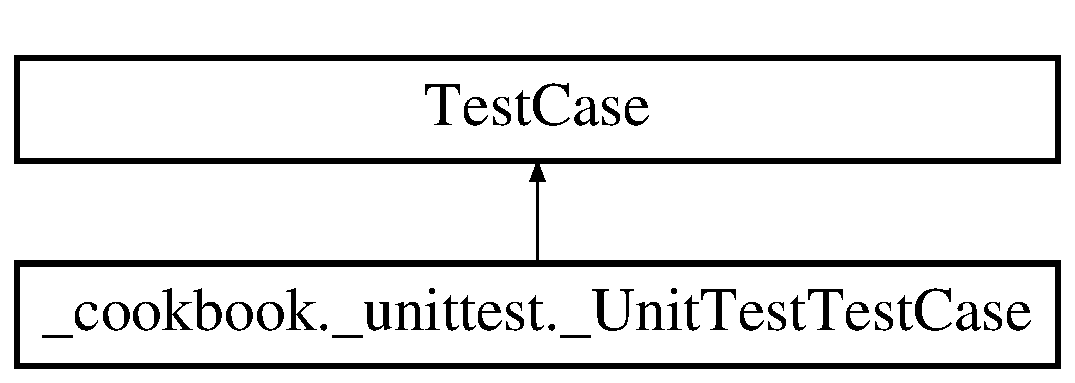
\includegraphics[height=2.000000cm]{dd/dfd/class__cookbook_1_1__unittest_1_1__UnitTestTestCase}
\end{center}
\end{figure}
\subsection*{Public Member Functions}
\begin{DoxyCompactItemize}
\item 
def \hyperlink{class__cookbook_1_1__unittest_1_1__UnitTestTestCase_ad6b68e36d804273afb8eb2aa1b79ba74}{set\-Up}
\item 
def \hyperlink{class__cookbook_1_1__unittest_1_1__UnitTestTestCase_a91e1c0f3653bce92280320c4d31110cb}{tear\-Down}
\item 
def \hyperlink{class__cookbook_1_1__unittest_1_1__UnitTestTestCase_a18f8f6f8b79b5d074ad2e01ea4944707}{test\-\_\-func\-\_\-1}
\item 
def \hyperlink{class__cookbook_1_1__unittest_1_1__UnitTestTestCase_a9a921e81044cde0239d1e5eaf43bbe9c}{test\-\_\-func\-\_\-2}
\item 
def \hyperlink{class__cookbook_1_1__unittest_1_1__UnitTestTestCase_a970636078c93003962607406a22276e8}{test\-\_\-func\-\_\-3}
\end{DoxyCompactItemize}


\subsection{Detailed Description}


Definition at line 77 of file \-\_\-unittest.\-py.



\subsection{Member Function Documentation}
\hypertarget{class__cookbook_1_1__unittest_1_1__UnitTestTestCase_ad6b68e36d804273afb8eb2aa1b79ba74}{\index{\-\_\-cookbook\-::\-\_\-unittest\-::\-\_\-\-Unit\-Test\-Test\-Case@{\-\_\-cookbook\-::\-\_\-unittest\-::\-\_\-\-Unit\-Test\-Test\-Case}!set\-Up@{set\-Up}}
\index{set\-Up@{set\-Up}!_cookbook::_unittest::_UnitTestTestCase@{\-\_\-cookbook\-::\-\_\-unittest\-::\-\_\-\-Unit\-Test\-Test\-Case}}
\subsubsection[{set\-Up}]{\setlength{\rightskip}{0pt plus 5cm}def \-\_\-cookbook.\-\_\-unittest.\-\_\-\-Unit\-Test\-Test\-Case.\-set\-Up (
\begin{DoxyParamCaption}
\item[{}]{self}
\end{DoxyParamCaption}
)}}\label{class__cookbook_1_1__unittest_1_1__UnitTestTestCase_ad6b68e36d804273afb8eb2aa1b79ba74}


Definition at line 78 of file \-\_\-unittest.\-py.

\hypertarget{class__cookbook_1_1__unittest_1_1__UnitTestTestCase_a91e1c0f3653bce92280320c4d31110cb}{\index{\-\_\-cookbook\-::\-\_\-unittest\-::\-\_\-\-Unit\-Test\-Test\-Case@{\-\_\-cookbook\-::\-\_\-unittest\-::\-\_\-\-Unit\-Test\-Test\-Case}!tear\-Down@{tear\-Down}}
\index{tear\-Down@{tear\-Down}!_cookbook::_unittest::_UnitTestTestCase@{\-\_\-cookbook\-::\-\_\-unittest\-::\-\_\-\-Unit\-Test\-Test\-Case}}
\subsubsection[{tear\-Down}]{\setlength{\rightskip}{0pt plus 5cm}def \-\_\-cookbook.\-\_\-unittest.\-\_\-\-Unit\-Test\-Test\-Case.\-tear\-Down (
\begin{DoxyParamCaption}
\item[{}]{self}
\end{DoxyParamCaption}
)}}\label{class__cookbook_1_1__unittest_1_1__UnitTestTestCase_a91e1c0f3653bce92280320c4d31110cb}


Definition at line 83 of file \-\_\-unittest.\-py.

\hypertarget{class__cookbook_1_1__unittest_1_1__UnitTestTestCase_a18f8f6f8b79b5d074ad2e01ea4944707}{\index{\-\_\-cookbook\-::\-\_\-unittest\-::\-\_\-\-Unit\-Test\-Test\-Case@{\-\_\-cookbook\-::\-\_\-unittest\-::\-\_\-\-Unit\-Test\-Test\-Case}!test\-\_\-func\-\_\-1@{test\-\_\-func\-\_\-1}}
\index{test\-\_\-func\-\_\-1@{test\-\_\-func\-\_\-1}!_cookbook::_unittest::_UnitTestTestCase@{\-\_\-cookbook\-::\-\_\-unittest\-::\-\_\-\-Unit\-Test\-Test\-Case}}
\subsubsection[{test\-\_\-func\-\_\-1}]{\setlength{\rightskip}{0pt plus 5cm}def \-\_\-cookbook.\-\_\-unittest.\-\_\-\-Unit\-Test\-Test\-Case.\-test\-\_\-func\-\_\-1 (
\begin{DoxyParamCaption}
\item[{}]{self}
\end{DoxyParamCaption}
)}}\label{class__cookbook_1_1__unittest_1_1__UnitTestTestCase_a18f8f6f8b79b5d074ad2e01ea4944707}


Definition at line 92 of file \-\_\-unittest.\-py.

\hypertarget{class__cookbook_1_1__unittest_1_1__UnitTestTestCase_a9a921e81044cde0239d1e5eaf43bbe9c}{\index{\-\_\-cookbook\-::\-\_\-unittest\-::\-\_\-\-Unit\-Test\-Test\-Case@{\-\_\-cookbook\-::\-\_\-unittest\-::\-\_\-\-Unit\-Test\-Test\-Case}!test\-\_\-func\-\_\-2@{test\-\_\-func\-\_\-2}}
\index{test\-\_\-func\-\_\-2@{test\-\_\-func\-\_\-2}!_cookbook::_unittest::_UnitTestTestCase@{\-\_\-cookbook\-::\-\_\-unittest\-::\-\_\-\-Unit\-Test\-Test\-Case}}
\subsubsection[{test\-\_\-func\-\_\-2}]{\setlength{\rightskip}{0pt plus 5cm}def \-\_\-cookbook.\-\_\-unittest.\-\_\-\-Unit\-Test\-Test\-Case.\-test\-\_\-func\-\_\-2 (
\begin{DoxyParamCaption}
\item[{}]{self}
\end{DoxyParamCaption}
)}}\label{class__cookbook_1_1__unittest_1_1__UnitTestTestCase_a9a921e81044cde0239d1e5eaf43bbe9c}


Definition at line 117 of file \-\_\-unittest.\-py.

\hypertarget{class__cookbook_1_1__unittest_1_1__UnitTestTestCase_a970636078c93003962607406a22276e8}{\index{\-\_\-cookbook\-::\-\_\-unittest\-::\-\_\-\-Unit\-Test\-Test\-Case@{\-\_\-cookbook\-::\-\_\-unittest\-::\-\_\-\-Unit\-Test\-Test\-Case}!test\-\_\-func\-\_\-3@{test\-\_\-func\-\_\-3}}
\index{test\-\_\-func\-\_\-3@{test\-\_\-func\-\_\-3}!_cookbook::_unittest::_UnitTestTestCase@{\-\_\-cookbook\-::\-\_\-unittest\-::\-\_\-\-Unit\-Test\-Test\-Case}}
\subsubsection[{test\-\_\-func\-\_\-3}]{\setlength{\rightskip}{0pt plus 5cm}def \-\_\-cookbook.\-\_\-unittest.\-\_\-\-Unit\-Test\-Test\-Case.\-test\-\_\-func\-\_\-3 (
\begin{DoxyParamCaption}
\item[{}]{self}
\end{DoxyParamCaption}
)}}\label{class__cookbook_1_1__unittest_1_1__UnitTestTestCase_a970636078c93003962607406a22276e8}


Definition at line 137 of file \-\_\-unittest.\-py.



The documentation for this class was generated from the following file\-:\begin{DoxyCompactItemize}
\item 
\-\_\-cookbook/\hyperlink{__unittest_8py}{\-\_\-unittest.\-py}\end{DoxyCompactItemize}

\hypertarget{class__cookbook_1_1OOP_1_1A}{\section{\-\_\-cookbook.\-O\-O\-P.\-A Class Reference}
\label{class__cookbook_1_1OOP_1_1A}\index{\-\_\-cookbook.\-O\-O\-P.\-A@{\-\_\-cookbook.\-O\-O\-P.\-A}}
}
Inheritance diagram for \-\_\-cookbook.\-O\-O\-P.\-A\-:\begin{figure}[H]
\begin{center}
\leavevmode
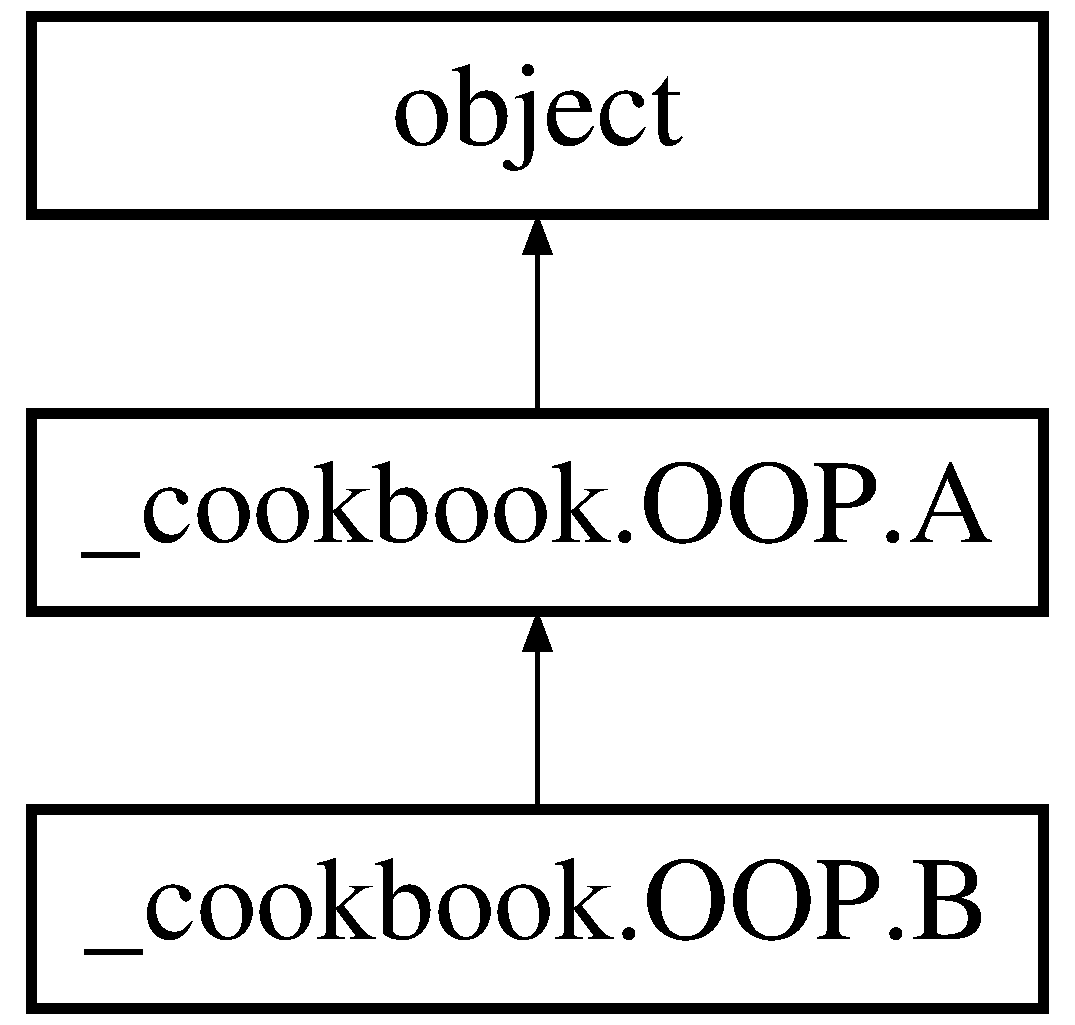
\includegraphics[height=3.000000cm]{d3/d8c/class__cookbook_1_1OOP_1_1A}
\end{center}
\end{figure}
\subsection*{Public Member Functions}
\begin{DoxyCompactItemize}
\item 
def \hyperlink{class__cookbook_1_1OOP_1_1A_aed1bb10487eebd0cba829be5e9572fde}{\-\_\-\-\_\-init\-\_\-\-\_\-}
\item 
def \hyperlink{class__cookbook_1_1OOP_1_1A_a0d6fe46ab76e7c05b4678bc56711b8be}{public\-\_\-instance\-\_\-method}
\item 
def \hyperlink{class__cookbook_1_1OOP_1_1A_a53147a5118b4d97348912e8ed2a5e45a}{class\-\_\-method}
\end{DoxyCompactItemize}
\subsection*{Static Public Member Functions}
\begin{DoxyCompactItemize}
\item 
def \hyperlink{class__cookbook_1_1OOP_1_1A_a6a8b4be6f2fe4addd97735dc47bc3ced}{static\-\_\-method}
\end{DoxyCompactItemize}
\subsection*{Public Attributes}
\begin{DoxyCompactItemize}
\item 
\hyperlink{class__cookbook_1_1OOP_1_1A_a3ff5d9c90ff2e8a6cb22e6e031085b87}{public\-\_\-instance\-\_\-attribute}
\item 
\hyperlink{class__cookbook_1_1OOP_1_1A_ab13df620204437ce904e7d8d582dab9c}{private\-\_\-instance\-\_\-attribute}
\end{DoxyCompactItemize}
\subsection*{Static Public Attributes}
\begin{DoxyCompactItemize}
\item 
int \hyperlink{class__cookbook_1_1OOP_1_1A_a594d2919ad2a27c4ae18fa97efb6de64}{num\-\_\-of\-\_\-instances} = 0
\end{DoxyCompactItemize}
\subsection*{Private Member Functions}
\begin{DoxyCompactItemize}
\item 
def \hyperlink{class__cookbook_1_1OOP_1_1A_a69a4dd4967ce9266cdd5f55d9398eb2c}{\-\_\-private\-\_\-instance\-\_\-method}
\end{DoxyCompactItemize}


\subsection{Detailed Description}
\begin{DoxyVerb}A class.

    >>> assert isinstance(A(), A)\end{DoxyVerb}
 

Definition at line 59 of file O\-O\-P.\-py.



\subsection{Constructor \& Destructor Documentation}
\hypertarget{class__cookbook_1_1OOP_1_1A_aed1bb10487eebd0cba829be5e9572fde}{\index{\-\_\-cookbook\-::\-O\-O\-P\-::\-A@{\-\_\-cookbook\-::\-O\-O\-P\-::\-A}!\-\_\-\-\_\-init\-\_\-\-\_\-@{\-\_\-\-\_\-init\-\_\-\-\_\-}}
\index{\-\_\-\-\_\-init\-\_\-\-\_\-@{\-\_\-\-\_\-init\-\_\-\-\_\-}!_cookbook::OOP::A@{\-\_\-cookbook\-::\-O\-O\-P\-::\-A}}
\subsubsection[{\-\_\-\-\_\-init\-\_\-\-\_\-}]{\setlength{\rightskip}{0pt plus 5cm}def \-\_\-cookbook.\-O\-O\-P.\-A.\-\_\-\-\_\-init\-\_\-\-\_\- (
\begin{DoxyParamCaption}
\item[{}]{self, }
\item[{}]{a1 = {\ttfamily None}, }
\item[{}]{a2 = {\ttfamily None}}
\end{DoxyParamCaption}
)}}\label{class__cookbook_1_1OOP_1_1A_aed1bb10487eebd0cba829be5e9572fde}


Definition at line 71 of file O\-O\-P.\-py.



\subsection{Member Function Documentation}
\hypertarget{class__cookbook_1_1OOP_1_1A_a69a4dd4967ce9266cdd5f55d9398eb2c}{\index{\-\_\-cookbook\-::\-O\-O\-P\-::\-A@{\-\_\-cookbook\-::\-O\-O\-P\-::\-A}!\-\_\-private\-\_\-instance\-\_\-method@{\-\_\-private\-\_\-instance\-\_\-method}}
\index{\-\_\-private\-\_\-instance\-\_\-method@{\-\_\-private\-\_\-instance\-\_\-method}!_cookbook::OOP::A@{\-\_\-cookbook\-::\-O\-O\-P\-::\-A}}
\subsubsection[{\-\_\-private\-\_\-instance\-\_\-method}]{\setlength{\rightskip}{0pt plus 5cm}def \-\_\-cookbook.\-O\-O\-P.\-A.\-\_\-private\-\_\-instance\-\_\-method (
\begin{DoxyParamCaption}
\item[{}]{self}
\end{DoxyParamCaption}
)\hspace{0.3cm}{\ttfamily [private]}}}\label{class__cookbook_1_1OOP_1_1A_a69a4dd4967ce9266cdd5f55d9398eb2c}


Definition at line 83 of file O\-O\-P.\-py.

\hypertarget{class__cookbook_1_1OOP_1_1A_a53147a5118b4d97348912e8ed2a5e45a}{\index{\-\_\-cookbook\-::\-O\-O\-P\-::\-A@{\-\_\-cookbook\-::\-O\-O\-P\-::\-A}!class\-\_\-method@{class\-\_\-method}}
\index{class\-\_\-method@{class\-\_\-method}!_cookbook::OOP::A@{\-\_\-cookbook\-::\-O\-O\-P\-::\-A}}
\subsubsection[{class\-\_\-method}]{\setlength{\rightskip}{0pt plus 5cm}def \-\_\-cookbook.\-O\-O\-P.\-A.\-class\-\_\-method (
\begin{DoxyParamCaption}
\item[{}]{cls}
\end{DoxyParamCaption}
)}}\label{class__cookbook_1_1OOP_1_1A_a53147a5118b4d97348912e8ed2a5e45a}


Definition at line 93 of file O\-O\-P.\-py.

\hypertarget{class__cookbook_1_1OOP_1_1A_a0d6fe46ab76e7c05b4678bc56711b8be}{\index{\-\_\-cookbook\-::\-O\-O\-P\-::\-A@{\-\_\-cookbook\-::\-O\-O\-P\-::\-A}!public\-\_\-instance\-\_\-method@{public\-\_\-instance\-\_\-method}}
\index{public\-\_\-instance\-\_\-method@{public\-\_\-instance\-\_\-method}!_cookbook::OOP::A@{\-\_\-cookbook\-::\-O\-O\-P\-::\-A}}
\subsubsection[{public\-\_\-instance\-\_\-method}]{\setlength{\rightskip}{0pt plus 5cm}def \-\_\-cookbook.\-O\-O\-P.\-A.\-public\-\_\-instance\-\_\-method (
\begin{DoxyParamCaption}
\item[{}]{self}
\end{DoxyParamCaption}
)}}\label{class__cookbook_1_1OOP_1_1A_a0d6fe46ab76e7c05b4678bc56711b8be}


Definition at line 77 of file O\-O\-P.\-py.

\hypertarget{class__cookbook_1_1OOP_1_1A_a6a8b4be6f2fe4addd97735dc47bc3ced}{\index{\-\_\-cookbook\-::\-O\-O\-P\-::\-A@{\-\_\-cookbook\-::\-O\-O\-P\-::\-A}!static\-\_\-method@{static\-\_\-method}}
\index{static\-\_\-method@{static\-\_\-method}!_cookbook::OOP::A@{\-\_\-cookbook\-::\-O\-O\-P\-::\-A}}
\subsubsection[{static\-\_\-method}]{\setlength{\rightskip}{0pt plus 5cm}def \-\_\-cookbook.\-O\-O\-P.\-A.\-static\-\_\-method (
\begin{DoxyParamCaption}
{}
\end{DoxyParamCaption}
)\hspace{0.3cm}{\ttfamily [static]}}}\label{class__cookbook_1_1OOP_1_1A_a6a8b4be6f2fe4addd97735dc47bc3ced}


Definition at line 88 of file O\-O\-P.\-py.



\subsection{Member Data Documentation}
\hypertarget{class__cookbook_1_1OOP_1_1A_a594d2919ad2a27c4ae18fa97efb6de64}{\index{\-\_\-cookbook\-::\-O\-O\-P\-::\-A@{\-\_\-cookbook\-::\-O\-O\-P\-::\-A}!num\-\_\-of\-\_\-instances@{num\-\_\-of\-\_\-instances}}
\index{num\-\_\-of\-\_\-instances@{num\-\_\-of\-\_\-instances}!_cookbook::OOP::A@{\-\_\-cookbook\-::\-O\-O\-P\-::\-A}}
\subsubsection[{num\-\_\-of\-\_\-instances}]{\setlength{\rightskip}{0pt plus 5cm}int \-\_\-cookbook.\-O\-O\-P.\-A.\-num\-\_\-of\-\_\-instances = 0\hspace{0.3cm}{\ttfamily [static]}}}\label{class__cookbook_1_1OOP_1_1A_a594d2919ad2a27c4ae18fa97efb6de64}


Definition at line 69 of file O\-O\-P.\-py.

\hypertarget{class__cookbook_1_1OOP_1_1A_ab13df620204437ce904e7d8d582dab9c}{\index{\-\_\-cookbook\-::\-O\-O\-P\-::\-A@{\-\_\-cookbook\-::\-O\-O\-P\-::\-A}!private\-\_\-instance\-\_\-attribute@{private\-\_\-instance\-\_\-attribute}}
\index{private\-\_\-instance\-\_\-attribute@{private\-\_\-instance\-\_\-attribute}!_cookbook::OOP::A@{\-\_\-cookbook\-::\-O\-O\-P\-::\-A}}
\subsubsection[{private\-\_\-instance\-\_\-attribute}]{\setlength{\rightskip}{0pt plus 5cm}\-\_\-cookbook.\-O\-O\-P.\-A.\-private\-\_\-instance\-\_\-attribute}}\label{class__cookbook_1_1OOP_1_1A_ab13df620204437ce904e7d8d582dab9c}


Definition at line 74 of file O\-O\-P.\-py.

\hypertarget{class__cookbook_1_1OOP_1_1A_a3ff5d9c90ff2e8a6cb22e6e031085b87}{\index{\-\_\-cookbook\-::\-O\-O\-P\-::\-A@{\-\_\-cookbook\-::\-O\-O\-P\-::\-A}!public\-\_\-instance\-\_\-attribute@{public\-\_\-instance\-\_\-attribute}}
\index{public\-\_\-instance\-\_\-attribute@{public\-\_\-instance\-\_\-attribute}!_cookbook::OOP::A@{\-\_\-cookbook\-::\-O\-O\-P\-::\-A}}
\subsubsection[{public\-\_\-instance\-\_\-attribute}]{\setlength{\rightskip}{0pt plus 5cm}\-\_\-cookbook.\-O\-O\-P.\-A.\-public\-\_\-instance\-\_\-attribute}}\label{class__cookbook_1_1OOP_1_1A_a3ff5d9c90ff2e8a6cb22e6e031085b87}


Definition at line 73 of file O\-O\-P.\-py.



The documentation for this class was generated from the following file\-:\begin{DoxyCompactItemize}
\item 
\-\_\-cookbook/\hyperlink{OOP_8py}{O\-O\-P.\-py}\end{DoxyCompactItemize}

\hypertarget{classadmin_1_1AdminError}{\section{admin.\-Admin\-Error Class Reference}
\label{classadmin_1_1AdminError}\index{admin.\-Admin\-Error@{admin.\-Admin\-Error}}
}


admin error  


Inheritance diagram for admin.\-Admin\-Error\-:\begin{figure}[H]
\begin{center}
\leavevmode
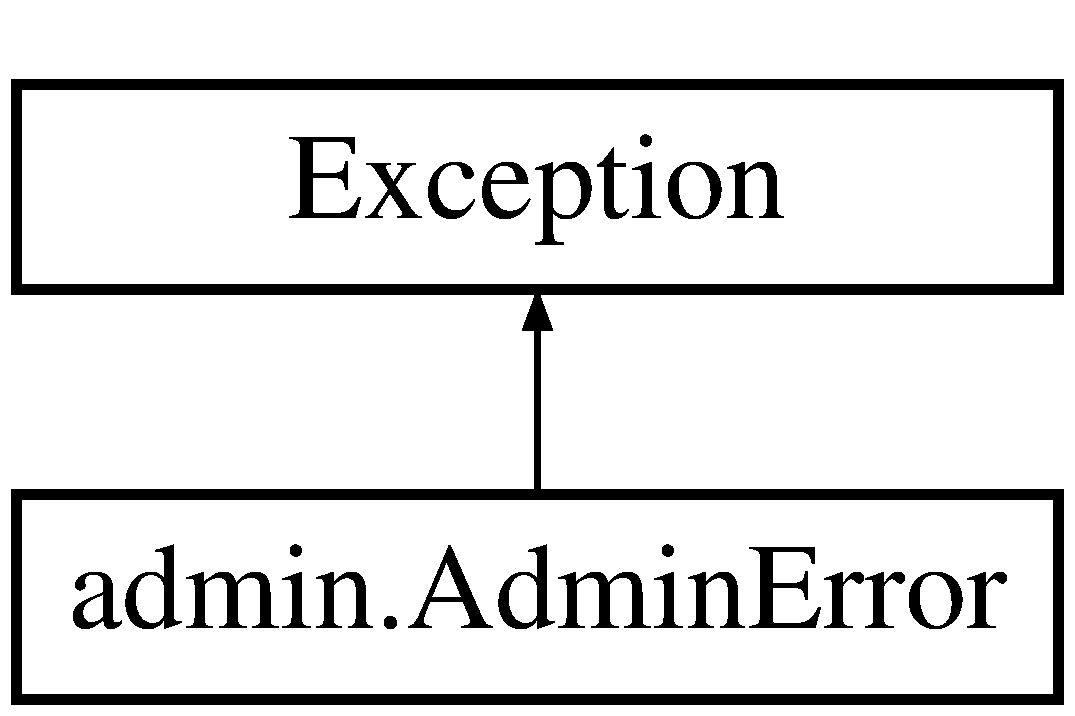
\includegraphics[height=2.000000cm]{df/dee/classadmin_1_1AdminError}
\end{center}
\end{figure}
\subsection*{Public Member Functions}
\begin{DoxyCompactItemize}
\item 
def \hyperlink{classadmin_1_1AdminError_a2712ee3b794fa425e6e0eac6a1524749}{\-\_\-\-\_\-init\-\_\-\-\_\-}
\item 
def \hyperlink{classadmin_1_1AdminError_ab64b4ac0bacc03d3f5d4dc556a493445}{\-\_\-\-\_\-str\-\_\-\-\_\-}
\end{DoxyCompactItemize}
\subsection*{Public Attributes}
\begin{DoxyCompactItemize}
\item 
\hyperlink{classadmin_1_1AdminError_a2d3933c27c7f643bf649f9f208f35c72}{error}
\end{DoxyCompactItemize}


\subsection{Detailed Description}
admin error 

Definition at line 45 of file admin.\-py.



\subsection{Constructor \& Destructor Documentation}
\hypertarget{classadmin_1_1AdminError_a2712ee3b794fa425e6e0eac6a1524749}{\index{admin\-::\-Admin\-Error@{admin\-::\-Admin\-Error}!\-\_\-\-\_\-init\-\_\-\-\_\-@{\-\_\-\-\_\-init\-\_\-\-\_\-}}
\index{\-\_\-\-\_\-init\-\_\-\-\_\-@{\-\_\-\-\_\-init\-\_\-\-\_\-}!admin::AdminError@{admin\-::\-Admin\-Error}}
\subsubsection[{\-\_\-\-\_\-init\-\_\-\-\_\-}]{\setlength{\rightskip}{0pt plus 5cm}def admin.\-Admin\-Error.\-\_\-\-\_\-init\-\_\-\-\_\- (
\begin{DoxyParamCaption}
\item[{}]{self, }
\item[{}]{e}
\end{DoxyParamCaption}
)}}\label{classadmin_1_1AdminError_a2712ee3b794fa425e6e0eac6a1524749}


Definition at line 46 of file admin.\-py.



\subsection{Member Function Documentation}
\hypertarget{classadmin_1_1AdminError_ab64b4ac0bacc03d3f5d4dc556a493445}{\index{admin\-::\-Admin\-Error@{admin\-::\-Admin\-Error}!\-\_\-\-\_\-str\-\_\-\-\_\-@{\-\_\-\-\_\-str\-\_\-\-\_\-}}
\index{\-\_\-\-\_\-str\-\_\-\-\_\-@{\-\_\-\-\_\-str\-\_\-\-\_\-}!admin::AdminError@{admin\-::\-Admin\-Error}}
\subsubsection[{\-\_\-\-\_\-str\-\_\-\-\_\-}]{\setlength{\rightskip}{0pt plus 5cm}def admin.\-Admin\-Error.\-\_\-\-\_\-str\-\_\-\-\_\- (
\begin{DoxyParamCaption}
\item[{}]{self}
\end{DoxyParamCaption}
)}}\label{classadmin_1_1AdminError_ab64b4ac0bacc03d3f5d4dc556a493445}


Definition at line 50 of file admin.\-py.



\subsection{Member Data Documentation}
\hypertarget{classadmin_1_1AdminError_a2d3933c27c7f643bf649f9f208f35c72}{\index{admin\-::\-Admin\-Error@{admin\-::\-Admin\-Error}!error@{error}}
\index{error@{error}!admin::AdminError@{admin\-::\-Admin\-Error}}
\subsubsection[{error}]{\setlength{\rightskip}{0pt plus 5cm}admin.\-Admin\-Error.\-error}}\label{classadmin_1_1AdminError_a2d3933c27c7f643bf649f9f208f35c72}


Definition at line 47 of file admin.\-py.



The documentation for this class was generated from the following file\-:\begin{DoxyCompactItemize}
\item 
\hyperlink{admin_8py}{admin.\-py}\end{DoxyCompactItemize}

\hypertarget{class__cookbook_1_1sort_1_1App}{\section{\-\_\-cookbook.\-sort.\-App Class Reference}
\label{class__cookbook_1_1sort_1_1App}\index{\-\_\-cookbook.\-sort.\-App@{\-\_\-cookbook.\-sort.\-App}}
}
\subsection*{Public Member Functions}
\begin{DoxyCompactItemize}
\item 
def \hyperlink{class__cookbook_1_1sort_1_1App_aff3e2e7895fa2533022a082dd8a3673c}{\-\_\-\-\_\-init\-\_\-\-\_\-}
\end{DoxyCompactItemize}
\subsection*{Public Attributes}
\begin{DoxyCompactItemize}
\item 
\hyperlink{class__cookbook_1_1sort_1_1App_a74df76f89c114157d3d2c375618fa124}{id}
\end{DoxyCompactItemize}


\subsection{Detailed Description}


Definition at line 93 of file sort.\-py.



\subsection{Constructor \& Destructor Documentation}
\hypertarget{class__cookbook_1_1sort_1_1App_aff3e2e7895fa2533022a082dd8a3673c}{\index{\-\_\-cookbook\-::sort\-::\-App@{\-\_\-cookbook\-::sort\-::\-App}!\-\_\-\-\_\-init\-\_\-\-\_\-@{\-\_\-\-\_\-init\-\_\-\-\_\-}}
\index{\-\_\-\-\_\-init\-\_\-\-\_\-@{\-\_\-\-\_\-init\-\_\-\-\_\-}!_cookbook::sort::App@{\-\_\-cookbook\-::sort\-::\-App}}
\subsubsection[{\-\_\-\-\_\-init\-\_\-\-\_\-}]{\setlength{\rightskip}{0pt plus 5cm}def \-\_\-cookbook.\-sort.\-App.\-\_\-\-\_\-init\-\_\-\-\_\- (
\begin{DoxyParamCaption}
\item[{}]{self, }
\item[{}]{id}
\end{DoxyParamCaption}
)}}\label{class__cookbook_1_1sort_1_1App_aff3e2e7895fa2533022a082dd8a3673c}


Definition at line 94 of file sort.\-py.



\subsection{Member Data Documentation}
\hypertarget{class__cookbook_1_1sort_1_1App_a74df76f89c114157d3d2c375618fa124}{\index{\-\_\-cookbook\-::sort\-::\-App@{\-\_\-cookbook\-::sort\-::\-App}!id@{id}}
\index{id@{id}!_cookbook::sort::App@{\-\_\-cookbook\-::sort\-::\-App}}
\subsubsection[{id}]{\setlength{\rightskip}{0pt plus 5cm}\-\_\-cookbook.\-sort.\-App.\-id}}\label{class__cookbook_1_1sort_1_1App_a74df76f89c114157d3d2c375618fa124}


Definition at line 95 of file sort.\-py.



The documentation for this class was generated from the following file\-:\begin{DoxyCompactItemize}
\item 
\-\_\-cookbook/\hyperlink{sort_8py}{sort.\-py}\end{DoxyCompactItemize}

\hypertarget{class__cookbook_1_1OOP_1_1B}{\section{\-\_\-cookbook.\-O\-O\-P.\-B Class Reference}
\label{class__cookbook_1_1OOP_1_1B}\index{\-\_\-cookbook.\-O\-O\-P.\-B@{\-\_\-cookbook.\-O\-O\-P.\-B}}
}
Inheritance diagram for \-\_\-cookbook.\-O\-O\-P.\-B\-:\begin{figure}[H]
\begin{center}
\leavevmode
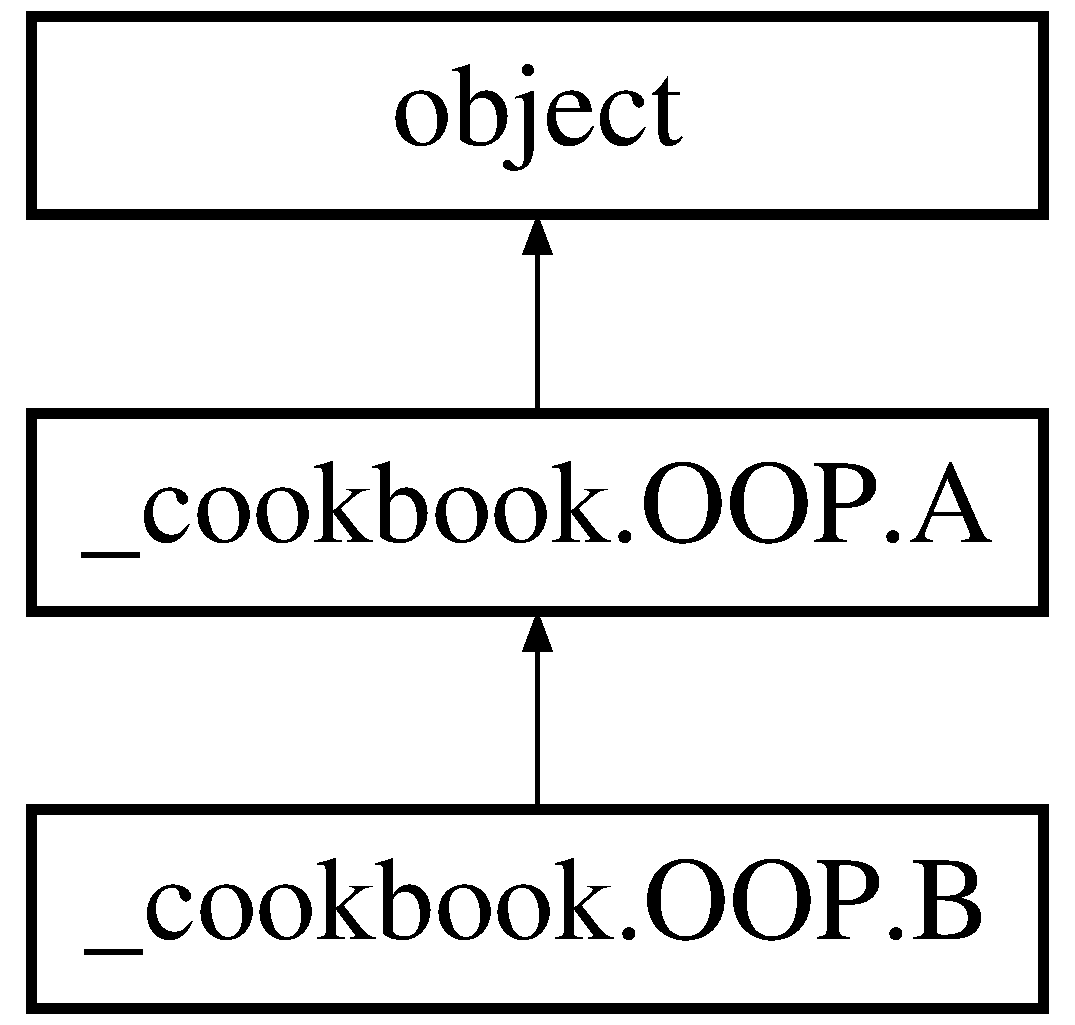
\includegraphics[height=3.000000cm]{d1/d62/class__cookbook_1_1OOP_1_1B}
\end{center}
\end{figure}
\subsection*{Public Member Functions}
\begin{DoxyCompactItemize}
\item 
def \hyperlink{class__cookbook_1_1OOP_1_1B_a9f3c49f91e93d0cfe607e9046b100c43}{\-\_\-\-\_\-init\-\_\-\-\_\-}
\item 
def \hyperlink{class__cookbook_1_1OOP_1_1B_aabb3a6d83ad9d362a6b88fbdd270d4f0}{public\-\_\-instance\-\_\-method}
\item 
def \hyperlink{class__cookbook_1_1OOP_1_1B_aa55b30a2f61c6106811984627635d98c}{new\-\_\-method}
\end{DoxyCompactItemize}
\subsection*{Public Attributes}
\begin{DoxyCompactItemize}
\item 
\hyperlink{class__cookbook_1_1OOP_1_1B_a19d2deae2721c44646f69f1718a1c2b4}{b}
\end{DoxyCompactItemize}
\subsection*{Additional Inherited Members}


\subsection{Detailed Description}
\begin{DoxyVerb}Subclass of A.

    >>> assert issubclass(B ,A)\end{DoxyVerb}
 

Definition at line 97 of file O\-O\-P.\-py.



\subsection{Constructor \& Destructor Documentation}
\hypertarget{class__cookbook_1_1OOP_1_1B_a9f3c49f91e93d0cfe607e9046b100c43}{\index{\-\_\-cookbook\-::\-O\-O\-P\-::\-B@{\-\_\-cookbook\-::\-O\-O\-P\-::\-B}!\-\_\-\-\_\-init\-\_\-\-\_\-@{\-\_\-\-\_\-init\-\_\-\-\_\-}}
\index{\-\_\-\-\_\-init\-\_\-\-\_\-@{\-\_\-\-\_\-init\-\_\-\-\_\-}!_cookbook::OOP::B@{\-\_\-cookbook\-::\-O\-O\-P\-::\-B}}
\subsubsection[{\-\_\-\-\_\-init\-\_\-\-\_\-}]{\setlength{\rightskip}{0pt plus 5cm}def \-\_\-cookbook.\-O\-O\-P.\-B.\-\_\-\-\_\-init\-\_\-\-\_\- (
\begin{DoxyParamCaption}
\item[{}]{self, }
\item[{}]{b, }
\item[{}]{a1 = {\ttfamily None}, }
\item[{}]{a2 = {\ttfamily None}}
\end{DoxyParamCaption}
)}}\label{class__cookbook_1_1OOP_1_1B_a9f3c49f91e93d0cfe607e9046b100c43}


Definition at line 104 of file O\-O\-P.\-py.



\subsection{Member Function Documentation}
\hypertarget{class__cookbook_1_1OOP_1_1B_aa55b30a2f61c6106811984627635d98c}{\index{\-\_\-cookbook\-::\-O\-O\-P\-::\-B@{\-\_\-cookbook\-::\-O\-O\-P\-::\-B}!new\-\_\-method@{new\-\_\-method}}
\index{new\-\_\-method@{new\-\_\-method}!_cookbook::OOP::B@{\-\_\-cookbook\-::\-O\-O\-P\-::\-B}}
\subsubsection[{new\-\_\-method}]{\setlength{\rightskip}{0pt plus 5cm}def \-\_\-cookbook.\-O\-O\-P.\-B.\-new\-\_\-method (
\begin{DoxyParamCaption}
\item[{}]{self}
\end{DoxyParamCaption}
)}}\label{class__cookbook_1_1OOP_1_1B_aa55b30a2f61c6106811984627635d98c}


Definition at line 113 of file O\-O\-P.\-py.

\hypertarget{class__cookbook_1_1OOP_1_1B_aabb3a6d83ad9d362a6b88fbdd270d4f0}{\index{\-\_\-cookbook\-::\-O\-O\-P\-::\-B@{\-\_\-cookbook\-::\-O\-O\-P\-::\-B}!public\-\_\-instance\-\_\-method@{public\-\_\-instance\-\_\-method}}
\index{public\-\_\-instance\-\_\-method@{public\-\_\-instance\-\_\-method}!_cookbook::OOP::B@{\-\_\-cookbook\-::\-O\-O\-P\-::\-B}}
\subsubsection[{public\-\_\-instance\-\_\-method}]{\setlength{\rightskip}{0pt plus 5cm}def \-\_\-cookbook.\-O\-O\-P.\-B.\-public\-\_\-instance\-\_\-method (
\begin{DoxyParamCaption}
\item[{}]{self}
\end{DoxyParamCaption}
)}}\label{class__cookbook_1_1OOP_1_1B_aabb3a6d83ad9d362a6b88fbdd270d4f0}


Definition at line 109 of file O\-O\-P.\-py.



\subsection{Member Data Documentation}
\hypertarget{class__cookbook_1_1OOP_1_1B_a19d2deae2721c44646f69f1718a1c2b4}{\index{\-\_\-cookbook\-::\-O\-O\-P\-::\-B@{\-\_\-cookbook\-::\-O\-O\-P\-::\-B}!b@{b}}
\index{b@{b}!_cookbook::OOP::B@{\-\_\-cookbook\-::\-O\-O\-P\-::\-B}}
\subsubsection[{b}]{\setlength{\rightskip}{0pt plus 5cm}\-\_\-cookbook.\-O\-O\-P.\-B.\-b}}\label{class__cookbook_1_1OOP_1_1B_a19d2deae2721c44646f69f1718a1c2b4}


Definition at line 106 of file O\-O\-P.\-py.



The documentation for this class was generated from the following file\-:\begin{DoxyCompactItemize}
\item 
\-\_\-cookbook/\hyperlink{OOP_8py}{O\-O\-P.\-py}\end{DoxyCompactItemize}

\hypertarget{classadmin_1_1build}{\section{admin.\-build Class Reference}
\label{classadmin_1_1build}\index{admin.\-build@{admin.\-build}}
}


Build tools.  


Inheritance diagram for admin.\-build\-:\begin{figure}[H]
\begin{center}
\leavevmode
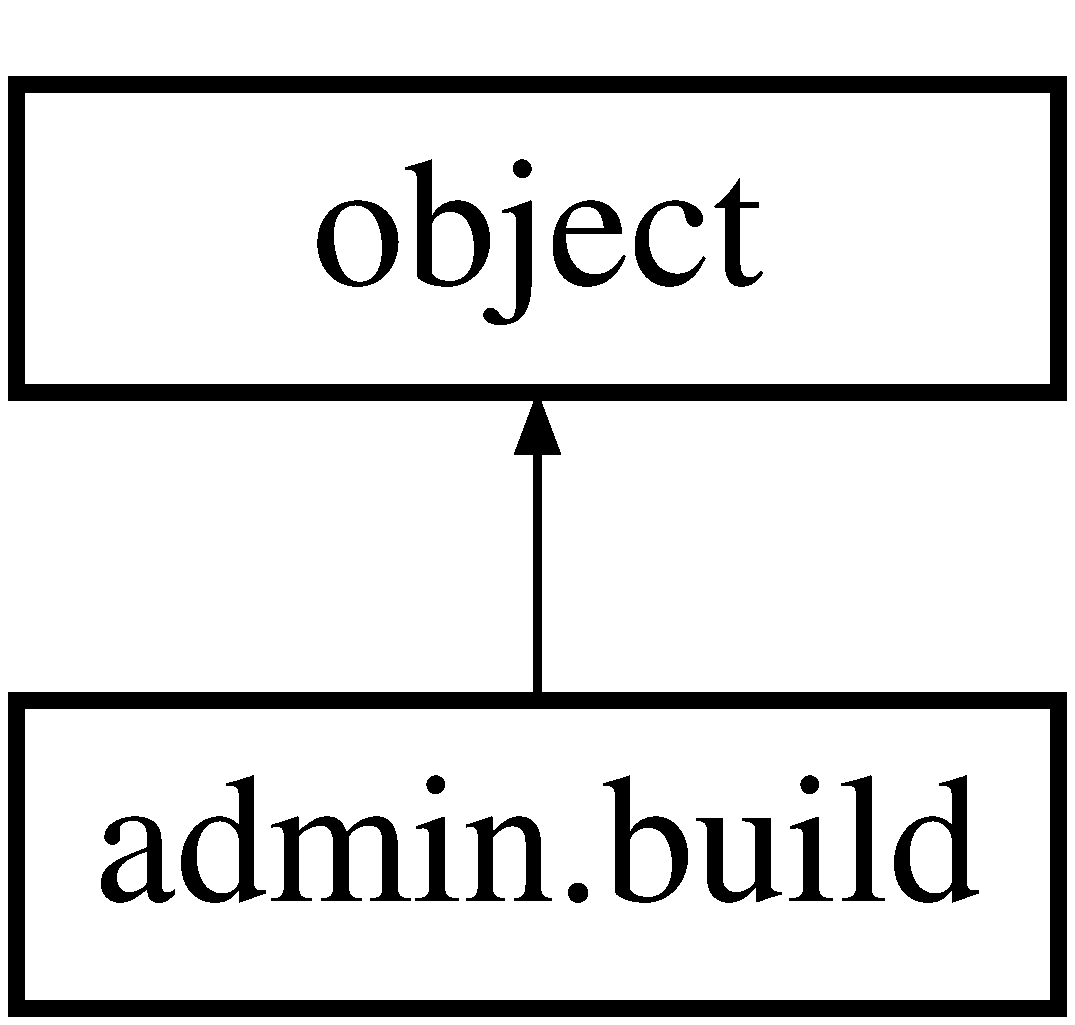
\includegraphics[height=2.000000cm]{d8/dff/classadmin_1_1build}
\end{center}
\end{figure}
\subsection*{Public Member Functions}
\begin{DoxyCompactItemize}
\item 
def \hyperlink{classadmin_1_1build_a265731c57c5b23175db096bf8a76e236}{decode\-\_\-version}
\begin{DoxyCompactList}\small\item\em Decode version information string. \end{DoxyCompactList}\item 
def \hyperlink{classadmin_1_1build_a119269530e1f9f01afc87834d21d722b}{match\-\_\-version}
\begin{DoxyCompactList}\small\item\em Match the specific version. \end{DoxyCompactList}\end{DoxyCompactItemize}
\subsection*{Static Public Member Functions}
\begin{DoxyCompactItemize}
\item 
def \hyperlink{classadmin_1_1build_add65d88734d0ae6b83e8c31cff366b68}{doxygen}
\begin{DoxyCompactList}\small\item\em Generate documentation for codes under Git by Doxygen. \end{DoxyCompactList}\end{DoxyCompactItemize}
\subsection*{Static Public Attributes}
\begin{DoxyCompactItemize}
\item 
tuple \hyperlink{classadmin_1_1build_acf6af7ed40a09ac4e0029edd50a82ae0}{Version} = namedtuple('Version', 'major, minor, patch')
\end{DoxyCompactItemize}


\subsection{Detailed Description}
Build tools. 

This module contains functions and classes for versions, including\-:


\begin{DoxyItemize}
\item Version
\item \hyperlink{classadmin_1_1build_a265731c57c5b23175db096bf8a76e236}{decode\-\_\-version()}, \hyperlink{classadmin_1_1build_a119269530e1f9f01afc87834d21d722b}{match\-\_\-version()} 
\end{DoxyItemize}

Definition at line 266 of file admin.\-py.



\subsection{Member Function Documentation}
\hypertarget{classadmin_1_1build_a265731c57c5b23175db096bf8a76e236}{\index{admin\-::build@{admin\-::build}!decode\-\_\-version@{decode\-\_\-version}}
\index{decode\-\_\-version@{decode\-\_\-version}!admin::build@{admin\-::build}}
\subsubsection[{decode\-\_\-version}]{\setlength{\rightskip}{0pt plus 5cm}def admin.\-build.\-decode\-\_\-version (
\begin{DoxyParamCaption}
\item[{}]{cls, }
\item[{}]{version\-\_\-info, }
\item[{}]{prefix = {\ttfamily ''}}
\end{DoxyParamCaption}
)}}\label{classadmin_1_1build_a265731c57c5b23175db096bf8a76e236}


Decode version information string. 


\begin{DoxyParams}{Parameters}
{\em version\-\_\-info} & version information string (e.\-g. Python 3.\-4.\-1) \\
\hline
{\em prefix} & prefix string of version \\
\hline
\end{DoxyParams}
\begin{DoxyReturn}{Returns}
Version named-\/tuple 
\end{DoxyReturn}


Definition at line 276 of file admin.\-py.

\hypertarget{classadmin_1_1build_add65d88734d0ae6b83e8c31cff366b68}{\index{admin\-::build@{admin\-::build}!doxygen@{doxygen}}
\index{doxygen@{doxygen}!admin::build@{admin\-::build}}
\subsubsection[{doxygen}]{\setlength{\rightskip}{0pt plus 5cm}def admin.\-build.\-doxygen (
\begin{DoxyParamCaption}
\item[{}]{path, }
\item[{}]{doxyfile = {\ttfamily 'Doxyfile.in'}}
\end{DoxyParamCaption}
)\hspace{0.3cm}{\ttfamily [static]}}}\label{classadmin_1_1build_add65d88734d0ae6b83e8c31cff366b68}


Generate documentation for codes under Git by Doxygen. 


\begin{DoxyParams}{Parameters}
{\em path} & project path \\
\hline
{\em doxyfile} & name of Doxygen configuration file \\
\hline
\end{DoxyParams}

\begin{DoxyExceptions}{Exceptions}
{\em subprocess.\-Called\-Process\-Error} & \\
\hline
{\em I\-O\-Error} & \\
\hline
\end{DoxyExceptions}
\begin{DoxySeeAlso}{See Also}
\href{http://www.stack.nl/~dimitri/doxygen/manual/}{\tt http\-://www.\-stack.\-nl/$\sim$dimitri/doxygen/manual/} 
\end{DoxySeeAlso}
\begin{DoxySince}{Since}
Doxygen 1.\-8.\-6 
\end{DoxySince}


Definition at line 318 of file admin.\-py.

\hypertarget{classadmin_1_1build_a119269530e1f9f01afc87834d21d722b}{\index{admin\-::build@{admin\-::build}!match\-\_\-version@{match\-\_\-version}}
\index{match\-\_\-version@{match\-\_\-version}!admin::build@{admin\-::build}}
\subsubsection[{match\-\_\-version}]{\setlength{\rightskip}{0pt plus 5cm}def admin.\-build.\-match\-\_\-version (
\begin{DoxyParamCaption}
\item[{}]{cls, }
\item[{}]{v, }
\item[{}]{match}
\end{DoxyParamCaption}
)}}\label{classadmin_1_1build_a119269530e1f9f01afc87834d21d722b}


Match the specific version. 


\begin{DoxyParams}{Parameters}
{\em v} & Version named-\/tuple \\
\hline
{\em match} & version string (e.\-g. 1.\-2.\-3) \\
\hline
\end{DoxyParams}
\begin{DoxyReturn}{Returns}
True if match 
\end{DoxyReturn}


Definition at line 296 of file admin.\-py.



\subsection{Member Data Documentation}
\hypertarget{classadmin_1_1build_acf6af7ed40a09ac4e0029edd50a82ae0}{\index{admin\-::build@{admin\-::build}!Version@{Version}}
\index{Version@{Version}!admin::build@{admin\-::build}}
\subsubsection[{Version}]{\setlength{\rightskip}{0pt plus 5cm}tuple admin.\-build.\-Version = namedtuple('Version', 'major, minor, patch')\hspace{0.3cm}{\ttfamily [static]}}}\label{classadmin_1_1build_acf6af7ed40a09ac4e0029edd50a82ae0}


Definition at line 268 of file admin.\-py.



The documentation for this class was generated from the following file\-:\begin{DoxyCompactItemize}
\item 
\hyperlink{admin_8py}{admin.\-py}\end{DoxyCompactItemize}

\hypertarget{classadmin_1_1ConfigFile}{\section{admin.\-Config\-File Class Reference}
\label{classadmin_1_1ConfigFile}\index{admin.\-Config\-File@{admin.\-Config\-File}}
}


Configuration file.  


Inheritance diagram for admin.\-Config\-File\-:\begin{figure}[H]
\begin{center}
\leavevmode
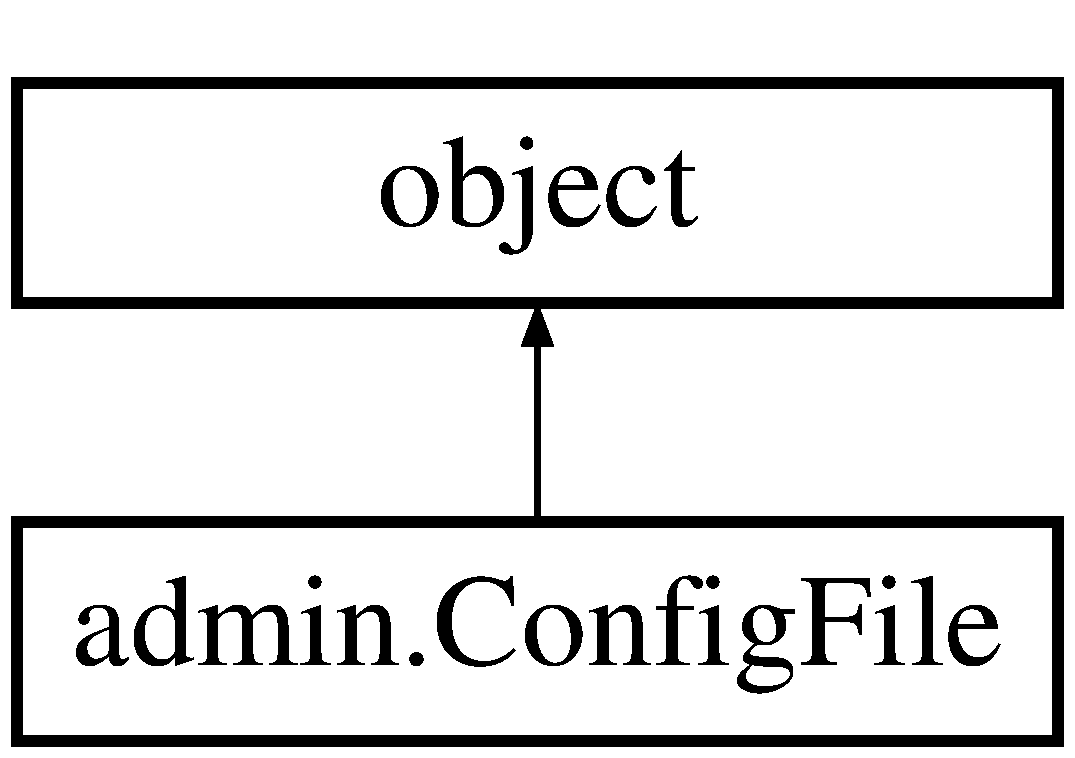
\includegraphics[height=2.000000cm]{d0/d8b/classadmin_1_1ConfigFile}
\end{center}
\end{figure}
\subsection*{Public Member Functions}
\begin{DoxyCompactItemize}
\item 
def \hyperlink{classadmin_1_1ConfigFile_a01f801b702c4cb7e322a8dee7943f5ff}{\-\_\-\-\_\-init\-\_\-\-\_\-}
\begin{DoxyCompactList}\small\item\em Parse configuration file. \end{DoxyCompactList}\item 
def \hyperlink{classadmin_1_1ConfigFile_a3a60d1611c929d782773d73d339454ab}{get}
\begin{DoxyCompactList}\small\item\em Get value of specific option. \end{DoxyCompactList}\item 
def \hyperlink{classadmin_1_1ConfigFile_a05413f3b3760fe95cf8038c400cb2b4f}{set}
\begin{DoxyCompactList}\small\item\em Set value of specific option. \end{DoxyCompactList}\end{DoxyCompactItemize}
\subsection*{Private Attributes}
\begin{DoxyCompactItemize}
\item 
\hyperlink{classadmin_1_1ConfigFile_ada03146a25635d360b9994efcd3eb6ce}{\-\_\-config\-\_\-file}
\item 
\hyperlink{classadmin_1_1ConfigFile_a3f7db562c59049e6a3b28b1fdfafa63e}{\-\_\-sep}
\item 
\hyperlink{classadmin_1_1ConfigFile_ac15829b16933412a7db88d3dacdcf345}{\-\_\-comments}
\item 
\hyperlink{classadmin_1_1ConfigFile_a5a5c415d13ee87e1a03c9f64231a4fc9}{\-\_\-config}
\end{DoxyCompactItemize}


\subsection{Detailed Description}
Configuration file. 

\subsubsection*{Usage}


\begin{DoxyPre}{\ttfamily 
     import os
     import admin}\end{DoxyPre}



\begin{DoxyPre}{\ttfamily      configs = \{'PROJECT\_NAME': '"AAA"',
           'PROJECT\_NUMBER': '1.2.3'\}
     try:
         with open(os.path.join(os.getcwd(), 'Doxyfile'), 'r+') as f:
             config\_file = \hyperlink{classadmin_1_1ConfigFile}{admin.ConfigFile(f)}
             config\_file.set(configs)
         except IOError as e:
             \hyperlink{namespaceadmin_ae1e80d1a965f6551fa95ff379ba2b0cd}{admin.error}('error') 
}\end{DoxyPre}


Definition at line 169 of file \-\_\-\-\_\-init\-\_\-\-\_\-.\-py.



\subsection{Constructor \& Destructor Documentation}
\hypertarget{classadmin_1_1ConfigFile_a01f801b702c4cb7e322a8dee7943f5ff}{\index{admin\-::\-Config\-File@{admin\-::\-Config\-File}!\-\_\-\-\_\-init\-\_\-\-\_\-@{\-\_\-\-\_\-init\-\_\-\-\_\-}}
\index{\-\_\-\-\_\-init\-\_\-\-\_\-@{\-\_\-\-\_\-init\-\_\-\-\_\-}!admin::ConfigFile@{admin\-::\-Config\-File}}
\subsubsection[{\-\_\-\-\_\-init\-\_\-\-\_\-}]{\setlength{\rightskip}{0pt plus 5cm}def admin.\-Config\-File.\-\_\-\-\_\-init\-\_\-\-\_\- (
\begin{DoxyParamCaption}
\item[{}]{self, }
\item[{}]{config\-\_\-file, }
\item[{}]{sep = {\ttfamily '='}, }
\item[{}]{comments = {\ttfamily '\#'}}
\end{DoxyParamCaption}
)}}\label{classadmin_1_1ConfigFile_a01f801b702c4cb7e322a8dee7943f5ff}


Parse configuration file. 


\begin{DoxyParams}{Parameters}
{\em config\-\_\-file} & configuration file object \\
\hline
{\em sep} & separator for option/value pair \\
\hline
{\em comments} & comments leading character \\
\hline
\end{DoxyParams}


Definition at line 175 of file \-\_\-\-\_\-init\-\_\-\-\_\-.\-py.



\subsection{Member Function Documentation}
\hypertarget{classadmin_1_1ConfigFile_a3a60d1611c929d782773d73d339454ab}{\index{admin\-::\-Config\-File@{admin\-::\-Config\-File}!get@{get}}
\index{get@{get}!admin::ConfigFile@{admin\-::\-Config\-File}}
\subsubsection[{get}]{\setlength{\rightskip}{0pt plus 5cm}def admin.\-Config\-File.\-get (
\begin{DoxyParamCaption}
\item[{}]{self, }
\item[{}]{option}
\end{DoxyParamCaption}
)}}\label{classadmin_1_1ConfigFile_a3a60d1611c929d782773d73d339454ab}


Get value of specific option. 


\begin{DoxyParams}{Parameters}
{\em option} & option name \\
\hline
\end{DoxyParams}
\begin{DoxyReturn}{Returns}
option value 
\end{DoxyReturn}

\begin{DoxyExceptions}{Exceptions}
{\em Key\-Error} & -\/ no optinon exists \\
\hline
\end{DoxyExceptions}


Definition at line 195 of file \-\_\-\-\_\-init\-\_\-\-\_\-.\-py.

\hypertarget{classadmin_1_1ConfigFile_a05413f3b3760fe95cf8038c400cb2b4f}{\index{admin\-::\-Config\-File@{admin\-::\-Config\-File}!set@{set}}
\index{set@{set}!admin::ConfigFile@{admin\-::\-Config\-File}}
\subsubsection[{set}]{\setlength{\rightskip}{0pt plus 5cm}def admin.\-Config\-File.\-set (
\begin{DoxyParamCaption}
\item[{}]{self, }
\item[{}]{pairs}
\end{DoxyParamCaption}
)}}\label{classadmin_1_1ConfigFile_a05413f3b3760fe95cf8038c400cb2b4f}


Set value of specific option. 


\begin{DoxyParams}{Parameters}
{\em pairs} & Pairs of option name-\/value. \\
\hline
\end{DoxyParams}


Definition at line 202 of file \-\_\-\-\_\-init\-\_\-\-\_\-.\-py.



\subsection{Member Data Documentation}
\hypertarget{classadmin_1_1ConfigFile_ac15829b16933412a7db88d3dacdcf345}{\index{admin\-::\-Config\-File@{admin\-::\-Config\-File}!\-\_\-comments@{\-\_\-comments}}
\index{\-\_\-comments@{\-\_\-comments}!admin::ConfigFile@{admin\-::\-Config\-File}}
\subsubsection[{\-\_\-comments}]{\setlength{\rightskip}{0pt plus 5cm}admin.\-Config\-File.\-\_\-comments\hspace{0.3cm}{\ttfamily [private]}}}\label{classadmin_1_1ConfigFile_ac15829b16933412a7db88d3dacdcf345}


Definition at line 178 of file \-\_\-\-\_\-init\-\_\-\-\_\-.\-py.

\hypertarget{classadmin_1_1ConfigFile_a5a5c415d13ee87e1a03c9f64231a4fc9}{\index{admin\-::\-Config\-File@{admin\-::\-Config\-File}!\-\_\-config@{\-\_\-config}}
\index{\-\_\-config@{\-\_\-config}!admin::ConfigFile@{admin\-::\-Config\-File}}
\subsubsection[{\-\_\-config}]{\setlength{\rightskip}{0pt plus 5cm}admin.\-Config\-File.\-\_\-config\hspace{0.3cm}{\ttfamily [private]}}}\label{classadmin_1_1ConfigFile_a5a5c415d13ee87e1a03c9f64231a4fc9}


Definition at line 179 of file \-\_\-\-\_\-init\-\_\-\-\_\-.\-py.

\hypertarget{classadmin_1_1ConfigFile_ada03146a25635d360b9994efcd3eb6ce}{\index{admin\-::\-Config\-File@{admin\-::\-Config\-File}!\-\_\-config\-\_\-file@{\-\_\-config\-\_\-file}}
\index{\-\_\-config\-\_\-file@{\-\_\-config\-\_\-file}!admin::ConfigFile@{admin\-::\-Config\-File}}
\subsubsection[{\-\_\-config\-\_\-file}]{\setlength{\rightskip}{0pt plus 5cm}admin.\-Config\-File.\-\_\-config\-\_\-file\hspace{0.3cm}{\ttfamily [private]}}}\label{classadmin_1_1ConfigFile_ada03146a25635d360b9994efcd3eb6ce}


Definition at line 176 of file \-\_\-\-\_\-init\-\_\-\-\_\-.\-py.

\hypertarget{classadmin_1_1ConfigFile_a3f7db562c59049e6a3b28b1fdfafa63e}{\index{admin\-::\-Config\-File@{admin\-::\-Config\-File}!\-\_\-sep@{\-\_\-sep}}
\index{\-\_\-sep@{\-\_\-sep}!admin::ConfigFile@{admin\-::\-Config\-File}}
\subsubsection[{\-\_\-sep}]{\setlength{\rightskip}{0pt plus 5cm}admin.\-Config\-File.\-\_\-sep\hspace{0.3cm}{\ttfamily [private]}}}\label{classadmin_1_1ConfigFile_a3f7db562c59049e6a3b28b1fdfafa63e}


Definition at line 177 of file \-\_\-\-\_\-init\-\_\-\-\_\-.\-py.



The documentation for this class was generated from the following file\-:\begin{DoxyCompactItemize}
\item 
admin/\hyperlink{____init_____8py}{\-\_\-\-\_\-init\-\_\-\-\_\-.\-py}\end{DoxyCompactItemize}

\hypertarget{class__cookbook_1_1thread_1_1__queue_1_1Cusumer}{\section{\-\_\-cookbook.\-thread.\-\_\-queue.\-Cusumer Class Reference}
\label{class__cookbook_1_1thread_1_1__queue_1_1Cusumer}\index{\-\_\-cookbook.\-thread.\-\_\-queue.\-Cusumer@{\-\_\-cookbook.\-thread.\-\_\-queue.\-Cusumer}}
}
Inheritance diagram for \-\_\-cookbook.\-thread.\-\_\-queue.\-Cusumer\-:\begin{figure}[H]
\begin{center}
\leavevmode
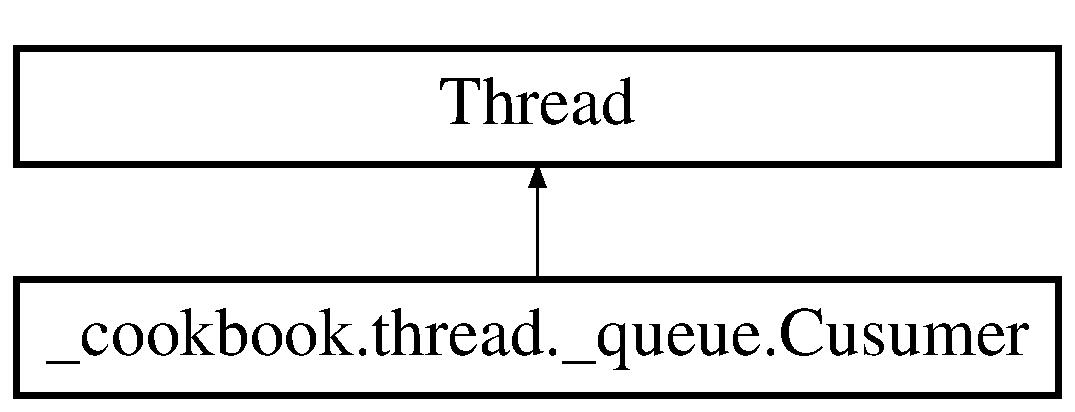
\includegraphics[height=2.000000cm]{df/dbf/class__cookbook_1_1thread_1_1__queue_1_1Cusumer}
\end{center}
\end{figure}
\subsection*{Public Member Functions}
\begin{DoxyCompactItemize}
\item 
def \hyperlink{class__cookbook_1_1thread_1_1__queue_1_1Cusumer_af05318b010b7ab9ddcf08b41c63f39f0}{\-\_\-\-\_\-init\-\_\-\-\_\-}
\item 
def \hyperlink{class__cookbook_1_1thread_1_1__queue_1_1Cusumer_ab96624a5b06833266094bf94920f9294}{run}
\end{DoxyCompactItemize}
\subsection*{Private Attributes}
\begin{DoxyCompactItemize}
\item 
\hyperlink{class__cookbook_1_1thread_1_1__queue_1_1Cusumer_a5113426d35d2d88365d4c024afdee3a4}{\-\_\-times}
\item 
\hyperlink{class__cookbook_1_1thread_1_1__queue_1_1Cusumer_aab1a86eae9f000baa8ee1e0883de0611}{\-\_\-item}
\end{DoxyCompactItemize}


\subsection{Detailed Description}


Definition at line 52 of file \-\_\-queue.\-py.



\subsection{Constructor \& Destructor Documentation}
\hypertarget{class__cookbook_1_1thread_1_1__queue_1_1Cusumer_af05318b010b7ab9ddcf08b41c63f39f0}{\index{\-\_\-cookbook\-::thread\-::\-\_\-queue\-::\-Cusumer@{\-\_\-cookbook\-::thread\-::\-\_\-queue\-::\-Cusumer}!\-\_\-\-\_\-init\-\_\-\-\_\-@{\-\_\-\-\_\-init\-\_\-\-\_\-}}
\index{\-\_\-\-\_\-init\-\_\-\-\_\-@{\-\_\-\-\_\-init\-\_\-\-\_\-}!_cookbook::thread::_queue::Cusumer@{\-\_\-cookbook\-::thread\-::\-\_\-queue\-::\-Cusumer}}
\subsubsection[{\-\_\-\-\_\-init\-\_\-\-\_\-}]{\setlength{\rightskip}{0pt plus 5cm}def \-\_\-cookbook.\-thread.\-\_\-queue.\-Cusumer.\-\_\-\-\_\-init\-\_\-\-\_\- (
\begin{DoxyParamCaption}
\item[{}]{self, }
\item[{}]{times = {\ttfamily 1}}
\end{DoxyParamCaption}
)}}\label{class__cookbook_1_1thread_1_1__queue_1_1Cusumer_af05318b010b7ab9ddcf08b41c63f39f0}


Definition at line 53 of file \-\_\-queue.\-py.



\subsection{Member Function Documentation}
\hypertarget{class__cookbook_1_1thread_1_1__queue_1_1Cusumer_ab96624a5b06833266094bf94920f9294}{\index{\-\_\-cookbook\-::thread\-::\-\_\-queue\-::\-Cusumer@{\-\_\-cookbook\-::thread\-::\-\_\-queue\-::\-Cusumer}!run@{run}}
\index{run@{run}!_cookbook::thread::_queue::Cusumer@{\-\_\-cookbook\-::thread\-::\-\_\-queue\-::\-Cusumer}}
\subsubsection[{run}]{\setlength{\rightskip}{0pt plus 5cm}def \-\_\-cookbook.\-thread.\-\_\-queue.\-Cusumer.\-run (
\begin{DoxyParamCaption}
\item[{}]{self}
\end{DoxyParamCaption}
)}}\label{class__cookbook_1_1thread_1_1__queue_1_1Cusumer_ab96624a5b06833266094bf94920f9294}


Definition at line 58 of file \-\_\-queue.\-py.



\subsection{Member Data Documentation}
\hypertarget{class__cookbook_1_1thread_1_1__queue_1_1Cusumer_aab1a86eae9f000baa8ee1e0883de0611}{\index{\-\_\-cookbook\-::thread\-::\-\_\-queue\-::\-Cusumer@{\-\_\-cookbook\-::thread\-::\-\_\-queue\-::\-Cusumer}!\-\_\-item@{\-\_\-item}}
\index{\-\_\-item@{\-\_\-item}!_cookbook::thread::_queue::Cusumer@{\-\_\-cookbook\-::thread\-::\-\_\-queue\-::\-Cusumer}}
\subsubsection[{\-\_\-item}]{\setlength{\rightskip}{0pt plus 5cm}\-\_\-cookbook.\-thread.\-\_\-queue.\-Cusumer.\-\_\-item\hspace{0.3cm}{\ttfamily [private]}}}\label{class__cookbook_1_1thread_1_1__queue_1_1Cusumer_aab1a86eae9f000baa8ee1e0883de0611}


Definition at line 56 of file \-\_\-queue.\-py.

\hypertarget{class__cookbook_1_1thread_1_1__queue_1_1Cusumer_a5113426d35d2d88365d4c024afdee3a4}{\index{\-\_\-cookbook\-::thread\-::\-\_\-queue\-::\-Cusumer@{\-\_\-cookbook\-::thread\-::\-\_\-queue\-::\-Cusumer}!\-\_\-times@{\-\_\-times}}
\index{\-\_\-times@{\-\_\-times}!_cookbook::thread::_queue::Cusumer@{\-\_\-cookbook\-::thread\-::\-\_\-queue\-::\-Cusumer}}
\subsubsection[{\-\_\-times}]{\setlength{\rightskip}{0pt plus 5cm}\-\_\-cookbook.\-thread.\-\_\-queue.\-Cusumer.\-\_\-times\hspace{0.3cm}{\ttfamily [private]}}}\label{class__cookbook_1_1thread_1_1__queue_1_1Cusumer_a5113426d35d2d88365d4c024afdee3a4}


Definition at line 55 of file \-\_\-queue.\-py.



The documentation for this class was generated from the following file\-:\begin{DoxyCompactItemize}
\item 
\-\_\-cookbook/thread/\hyperlink{__queue_8py}{\-\_\-queue.\-py}\end{DoxyCompactItemize}

\hypertarget{class__cookbook_1_1thread_1_1semaphore_1_1Cusumer}{\section{\-\_\-cookbook.\-thread.\-semaphore.\-Cusumer Class Reference}
\label{class__cookbook_1_1thread_1_1semaphore_1_1Cusumer}\index{\-\_\-cookbook.\-thread.\-semaphore.\-Cusumer@{\-\_\-cookbook.\-thread.\-semaphore.\-Cusumer}}
}
Inheritance diagram for \-\_\-cookbook.\-thread.\-semaphore.\-Cusumer\-:\begin{figure}[H]
\begin{center}
\leavevmode
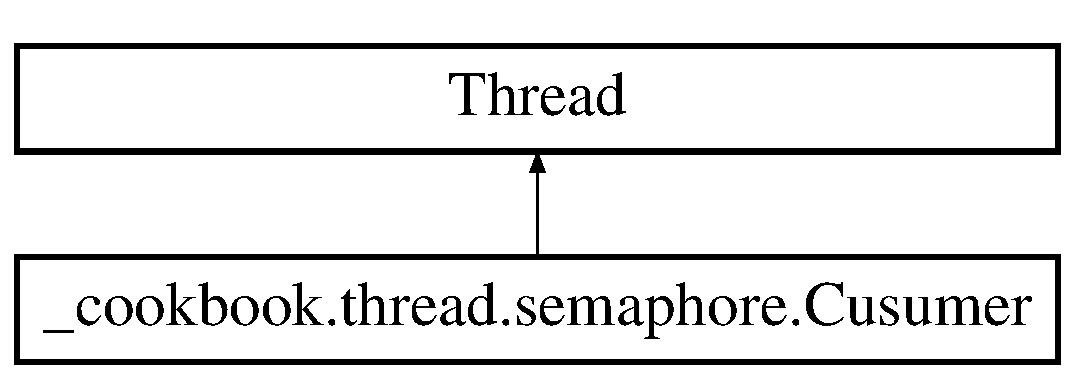
\includegraphics[height=2.000000cm]{de/dfa/class__cookbook_1_1thread_1_1semaphore_1_1Cusumer}
\end{center}
\end{figure}
\subsection*{Public Member Functions}
\begin{DoxyCompactItemize}
\item 
def \hyperlink{class__cookbook_1_1thread_1_1semaphore_1_1Cusumer_a2d0dfdb45b6d3e2e91ae80e813db1dc1}{\-\_\-\-\_\-init\-\_\-\-\_\-}
\item 
def \hyperlink{class__cookbook_1_1thread_1_1semaphore_1_1Cusumer_a6142eb28de70f5413dae68f02aef61e2}{run}
\end{DoxyCompactItemize}
\subsection*{Public Attributes}
\begin{DoxyCompactItemize}
\item 
\hyperlink{class__cookbook_1_1thread_1_1semaphore_1_1Cusumer_a7be67094634603b1b2a555144ad0c9aa}{arg}
\end{DoxyCompactItemize}


\subsection{Detailed Description}


Definition at line 58 of file semaphore.\-py.



\subsection{Constructor \& Destructor Documentation}
\hypertarget{class__cookbook_1_1thread_1_1semaphore_1_1Cusumer_a2d0dfdb45b6d3e2e91ae80e813db1dc1}{\index{\-\_\-cookbook\-::thread\-::semaphore\-::\-Cusumer@{\-\_\-cookbook\-::thread\-::semaphore\-::\-Cusumer}!\-\_\-\-\_\-init\-\_\-\-\_\-@{\-\_\-\-\_\-init\-\_\-\-\_\-}}
\index{\-\_\-\-\_\-init\-\_\-\-\_\-@{\-\_\-\-\_\-init\-\_\-\-\_\-}!_cookbook::thread::semaphore::Cusumer@{\-\_\-cookbook\-::thread\-::semaphore\-::\-Cusumer}}
\subsubsection[{\-\_\-\-\_\-init\-\_\-\-\_\-}]{\setlength{\rightskip}{0pt plus 5cm}def \-\_\-cookbook.\-thread.\-semaphore.\-Cusumer.\-\_\-\-\_\-init\-\_\-\-\_\- (
\begin{DoxyParamCaption}
\item[{}]{self}
\end{DoxyParamCaption}
)}}\label{class__cookbook_1_1thread_1_1semaphore_1_1Cusumer_a2d0dfdb45b6d3e2e91ae80e813db1dc1}


Definition at line 59 of file semaphore.\-py.



\subsection{Member Function Documentation}
\hypertarget{class__cookbook_1_1thread_1_1semaphore_1_1Cusumer_a6142eb28de70f5413dae68f02aef61e2}{\index{\-\_\-cookbook\-::thread\-::semaphore\-::\-Cusumer@{\-\_\-cookbook\-::thread\-::semaphore\-::\-Cusumer}!run@{run}}
\index{run@{run}!_cookbook::thread::semaphore::Cusumer@{\-\_\-cookbook\-::thread\-::semaphore\-::\-Cusumer}}
\subsubsection[{run}]{\setlength{\rightskip}{0pt plus 5cm}def \-\_\-cookbook.\-thread.\-semaphore.\-Cusumer.\-run (
\begin{DoxyParamCaption}
\item[{}]{self}
\end{DoxyParamCaption}
)}}\label{class__cookbook_1_1thread_1_1semaphore_1_1Cusumer_a6142eb28de70f5413dae68f02aef61e2}


Definition at line 64 of file semaphore.\-py.



\subsection{Member Data Documentation}
\hypertarget{class__cookbook_1_1thread_1_1semaphore_1_1Cusumer_a7be67094634603b1b2a555144ad0c9aa}{\index{\-\_\-cookbook\-::thread\-::semaphore\-::\-Cusumer@{\-\_\-cookbook\-::thread\-::semaphore\-::\-Cusumer}!arg@{arg}}
\index{arg@{arg}!_cookbook::thread::semaphore::Cusumer@{\-\_\-cookbook\-::thread\-::semaphore\-::\-Cusumer}}
\subsubsection[{arg}]{\setlength{\rightskip}{0pt plus 5cm}\-\_\-cookbook.\-thread.\-semaphore.\-Cusumer.\-arg}}\label{class__cookbook_1_1thread_1_1semaphore_1_1Cusumer_a7be67094634603b1b2a555144ad0c9aa}


Definition at line 61 of file semaphore.\-py.



The documentation for this class was generated from the following file\-:\begin{DoxyCompactItemize}
\item 
\-\_\-cookbook/thread/\hyperlink{semaphore_8py}{semaphore.\-py}\end{DoxyCompactItemize}

\hypertarget{class__cookbook_1_1context__manager_1_1MyContextManagerWithDecorator}{\section{\-\_\-cookbook.\-context\-\_\-manager.\-My\-Context\-Manager\-With\-Decorator Class Reference}
\label{class__cookbook_1_1context__manager_1_1MyContextManagerWithDecorator}\index{\-\_\-cookbook.\-context\-\_\-manager.\-My\-Context\-Manager\-With\-Decorator@{\-\_\-cookbook.\-context\-\_\-manager.\-My\-Context\-Manager\-With\-Decorator}}
}
Inheritance diagram for \-\_\-cookbook.\-context\-\_\-manager.\-My\-Context\-Manager\-With\-Decorator\-:\begin{figure}[H]
\begin{center}
\leavevmode
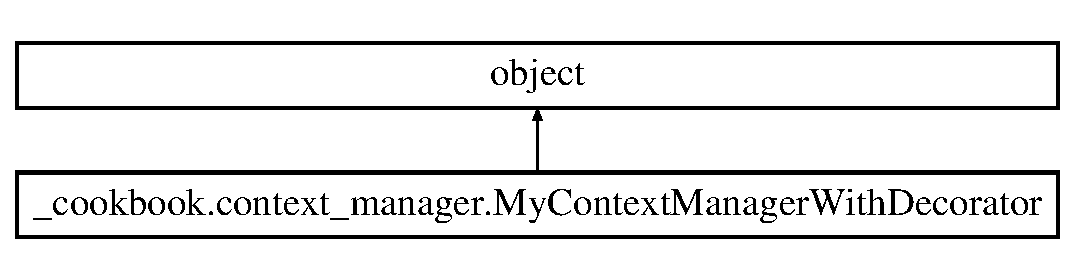
\includegraphics[height=2.000000cm]{d0/de7/class__cookbook_1_1context__manager_1_1MyContextManagerWithDecorator}
\end{center}
\end{figure}
\subsection*{Public Member Functions}
\begin{DoxyCompactItemize}
\item 
def \hyperlink{class__cookbook_1_1context__manager_1_1MyContextManagerWithDecorator_a0a4da720469cda83e496fc9803d3664e}{\-\_\-\-\_\-init\-\_\-\-\_\-}
\item 
def \hyperlink{class__cookbook_1_1context__manager_1_1MyContextManagerWithDecorator_a5434d93ea16adbacd9934eef6073963c}{close}
\item 
def \hyperlink{class__cookbook_1_1context__manager_1_1MyContextManagerWithDecorator_a8b22456b4212e6c458404aff36c68358}{do}
\end{DoxyCompactItemize}


\subsection{Detailed Description}


Definition at line 77 of file context\-\_\-manager.\-py.



\subsection{Constructor \& Destructor Documentation}
\hypertarget{class__cookbook_1_1context__manager_1_1MyContextManagerWithDecorator_a0a4da720469cda83e496fc9803d3664e}{\index{\-\_\-cookbook\-::context\-\_\-manager\-::\-My\-Context\-Manager\-With\-Decorator@{\-\_\-cookbook\-::context\-\_\-manager\-::\-My\-Context\-Manager\-With\-Decorator}!\-\_\-\-\_\-init\-\_\-\-\_\-@{\-\_\-\-\_\-init\-\_\-\-\_\-}}
\index{\-\_\-\-\_\-init\-\_\-\-\_\-@{\-\_\-\-\_\-init\-\_\-\-\_\-}!_cookbook::context_manager::MyContextManagerWithDecorator@{\-\_\-cookbook\-::context\-\_\-manager\-::\-My\-Context\-Manager\-With\-Decorator}}
\subsubsection[{\-\_\-\-\_\-init\-\_\-\-\_\-}]{\setlength{\rightskip}{0pt plus 5cm}def \-\_\-cookbook.\-context\-\_\-manager.\-My\-Context\-Manager\-With\-Decorator.\-\_\-\-\_\-init\-\_\-\-\_\- (
\begin{DoxyParamCaption}
\item[{}]{self, }
\item[{}]{ok = {\ttfamily True}}
\end{DoxyParamCaption}
)}}\label{class__cookbook_1_1context__manager_1_1MyContextManagerWithDecorator_a0a4da720469cda83e496fc9803d3664e}


Definition at line 78 of file context\-\_\-manager.\-py.



\subsection{Member Function Documentation}
\hypertarget{class__cookbook_1_1context__manager_1_1MyContextManagerWithDecorator_a5434d93ea16adbacd9934eef6073963c}{\index{\-\_\-cookbook\-::context\-\_\-manager\-::\-My\-Context\-Manager\-With\-Decorator@{\-\_\-cookbook\-::context\-\_\-manager\-::\-My\-Context\-Manager\-With\-Decorator}!close@{close}}
\index{close@{close}!_cookbook::context_manager::MyContextManagerWithDecorator@{\-\_\-cookbook\-::context\-\_\-manager\-::\-My\-Context\-Manager\-With\-Decorator}}
\subsubsection[{close}]{\setlength{\rightskip}{0pt plus 5cm}def \-\_\-cookbook.\-context\-\_\-manager.\-My\-Context\-Manager\-With\-Decorator.\-close (
\begin{DoxyParamCaption}
\item[{}]{self}
\end{DoxyParamCaption}
)}}\label{class__cookbook_1_1context__manager_1_1MyContextManagerWithDecorator_a5434d93ea16adbacd9934eef6073963c}


Definition at line 86 of file context\-\_\-manager.\-py.

\hypertarget{class__cookbook_1_1context__manager_1_1MyContextManagerWithDecorator_a8b22456b4212e6c458404aff36c68358}{\index{\-\_\-cookbook\-::context\-\_\-manager\-::\-My\-Context\-Manager\-With\-Decorator@{\-\_\-cookbook\-::context\-\_\-manager\-::\-My\-Context\-Manager\-With\-Decorator}!do@{do}}
\index{do@{do}!_cookbook::context_manager::MyContextManagerWithDecorator@{\-\_\-cookbook\-::context\-\_\-manager\-::\-My\-Context\-Manager\-With\-Decorator}}
\subsubsection[{do}]{\setlength{\rightskip}{0pt plus 5cm}def \-\_\-cookbook.\-context\-\_\-manager.\-My\-Context\-Manager\-With\-Decorator.\-do (
\begin{DoxyParamCaption}
\item[{}]{self, }
\item[{}]{ok = {\ttfamily True}}
\end{DoxyParamCaption}
)}}\label{class__cookbook_1_1context__manager_1_1MyContextManagerWithDecorator_a8b22456b4212e6c458404aff36c68358}


Definition at line 90 of file context\-\_\-manager.\-py.



The documentation for this class was generated from the following file\-:\begin{DoxyCompactItemize}
\item 
\-\_\-cookbook/\hyperlink{context__manager_8py}{context\-\_\-manager.\-py}\end{DoxyCompactItemize}

\hypertarget{class__cookbook_1_1loop_1_1MyIterator}{\section{\-\_\-cookbook.\-loop.\-My\-Iterator Class Reference}
\label{class__cookbook_1_1loop_1_1MyIterator}\index{\-\_\-cookbook.\-loop.\-My\-Iterator@{\-\_\-cookbook.\-loop.\-My\-Iterator}}
}
Inheritance diagram for \-\_\-cookbook.\-loop.\-My\-Iterator\-:\begin{figure}[H]
\begin{center}
\leavevmode
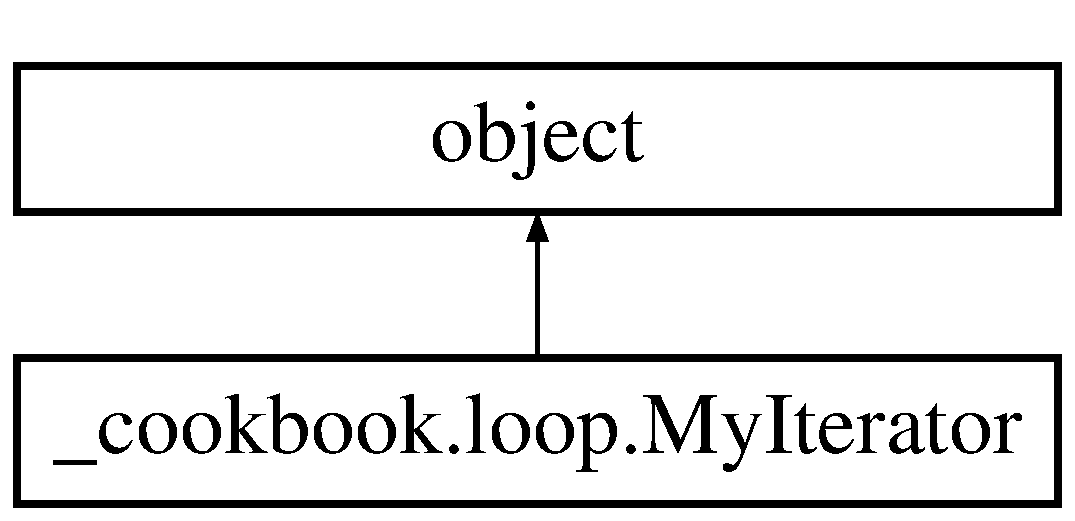
\includegraphics[height=2.000000cm]{d9/de3/class__cookbook_1_1loop_1_1MyIterator}
\end{center}
\end{figure}
\subsection*{Public Member Functions}
\begin{DoxyCompactItemize}
\item 
def \hyperlink{class__cookbook_1_1loop_1_1MyIterator_a0d22013198b99735cf506c1b783f2963}{\-\_\-\-\_\-init\-\_\-\-\_\-}
\item 
def \hyperlink{class__cookbook_1_1loop_1_1MyIterator_a41f8dca4e290ba0fd53ac547d448de1f}{\-\_\-\-\_\-iter\-\_\-\-\_\-}
\item 
def \hyperlink{class__cookbook_1_1loop_1_1MyIterator_ab9f3bae16f2426e6679df31ebbab766c}{\-\_\-\-\_\-next\-\_\-\-\_\-}
\end{DoxyCompactItemize}
\subsection*{Private Attributes}
\begin{DoxyCompactItemize}
\item 
\hyperlink{class__cookbook_1_1loop_1_1MyIterator_ac35e940f5d4704ce7fd0799d5affc2a2}{\-\_\-container}
\item 
\hyperlink{class__cookbook_1_1loop_1_1MyIterator_ad149ab2885a56c2a16b18800e91c5233}{\-\_\-index}
\end{DoxyCompactItemize}


\subsection{Detailed Description}
\begin{DoxyVerb}Iterator.

Python supports a concept of iteration over containers. This is
implemented using two distinct methods (`__iter__()`, and `next()`); these
are used to allow user-defined classes to support iteration.

To use it,

    >>> for i in MyIterator([1, 2, 3]):
    ...    print(i)
    1
    2
    3\end{DoxyVerb}
 

Definition at line 186 of file loop.\-py.



\subsection{Constructor \& Destructor Documentation}
\hypertarget{class__cookbook_1_1loop_1_1MyIterator_a0d22013198b99735cf506c1b783f2963}{\index{\-\_\-cookbook\-::loop\-::\-My\-Iterator@{\-\_\-cookbook\-::loop\-::\-My\-Iterator}!\-\_\-\-\_\-init\-\_\-\-\_\-@{\-\_\-\-\_\-init\-\_\-\-\_\-}}
\index{\-\_\-\-\_\-init\-\_\-\-\_\-@{\-\_\-\-\_\-init\-\_\-\-\_\-}!_cookbook::loop::MyIterator@{\-\_\-cookbook\-::loop\-::\-My\-Iterator}}
\subsubsection[{\-\_\-\-\_\-init\-\_\-\-\_\-}]{\setlength{\rightskip}{0pt plus 5cm}def \-\_\-cookbook.\-loop.\-My\-Iterator.\-\_\-\-\_\-init\-\_\-\-\_\- (
\begin{DoxyParamCaption}
\item[{}]{self, }
\item[{}]{seq}
\end{DoxyParamCaption}
)}}\label{class__cookbook_1_1loop_1_1MyIterator_a0d22013198b99735cf506c1b783f2963}


Definition at line 202 of file loop.\-py.



\subsection{Member Function Documentation}
\hypertarget{class__cookbook_1_1loop_1_1MyIterator_a41f8dca4e290ba0fd53ac547d448de1f}{\index{\-\_\-cookbook\-::loop\-::\-My\-Iterator@{\-\_\-cookbook\-::loop\-::\-My\-Iterator}!\-\_\-\-\_\-iter\-\_\-\-\_\-@{\-\_\-\-\_\-iter\-\_\-\-\_\-}}
\index{\-\_\-\-\_\-iter\-\_\-\-\_\-@{\-\_\-\-\_\-iter\-\_\-\-\_\-}!_cookbook::loop::MyIterator@{\-\_\-cookbook\-::loop\-::\-My\-Iterator}}
\subsubsection[{\-\_\-\-\_\-iter\-\_\-\-\_\-}]{\setlength{\rightskip}{0pt plus 5cm}def \-\_\-cookbook.\-loop.\-My\-Iterator.\-\_\-\-\_\-iter\-\_\-\-\_\- (
\begin{DoxyParamCaption}
\item[{}]{self}
\end{DoxyParamCaption}
)}}\label{class__cookbook_1_1loop_1_1MyIterator_a41f8dca4e290ba0fd53ac547d448de1f}


Definition at line 207 of file loop.\-py.

\hypertarget{class__cookbook_1_1loop_1_1MyIterator_ab9f3bae16f2426e6679df31ebbab766c}{\index{\-\_\-cookbook\-::loop\-::\-My\-Iterator@{\-\_\-cookbook\-::loop\-::\-My\-Iterator}!\-\_\-\-\_\-next\-\_\-\-\_\-@{\-\_\-\-\_\-next\-\_\-\-\_\-}}
\index{\-\_\-\-\_\-next\-\_\-\-\_\-@{\-\_\-\-\_\-next\-\_\-\-\_\-}!_cookbook::loop::MyIterator@{\-\_\-cookbook\-::loop\-::\-My\-Iterator}}
\subsubsection[{\-\_\-\-\_\-next\-\_\-\-\_\-}]{\setlength{\rightskip}{0pt plus 5cm}def \-\_\-cookbook.\-loop.\-My\-Iterator.\-\_\-\-\_\-next\-\_\-\-\_\- (
\begin{DoxyParamCaption}
\item[{}]{self}
\end{DoxyParamCaption}
)}}\label{class__cookbook_1_1loop_1_1MyIterator_ab9f3bae16f2426e6679df31ebbab766c}


Definition at line 211 of file loop.\-py.



\subsection{Member Data Documentation}
\hypertarget{class__cookbook_1_1loop_1_1MyIterator_ac35e940f5d4704ce7fd0799d5affc2a2}{\index{\-\_\-cookbook\-::loop\-::\-My\-Iterator@{\-\_\-cookbook\-::loop\-::\-My\-Iterator}!\-\_\-container@{\-\_\-container}}
\index{\-\_\-container@{\-\_\-container}!_cookbook::loop::MyIterator@{\-\_\-cookbook\-::loop\-::\-My\-Iterator}}
\subsubsection[{\-\_\-container}]{\setlength{\rightskip}{0pt plus 5cm}\-\_\-cookbook.\-loop.\-My\-Iterator.\-\_\-container\hspace{0.3cm}{\ttfamily [private]}}}\label{class__cookbook_1_1loop_1_1MyIterator_ac35e940f5d4704ce7fd0799d5affc2a2}


Definition at line 203 of file loop.\-py.

\hypertarget{class__cookbook_1_1loop_1_1MyIterator_ad149ab2885a56c2a16b18800e91c5233}{\index{\-\_\-cookbook\-::loop\-::\-My\-Iterator@{\-\_\-cookbook\-::loop\-::\-My\-Iterator}!\-\_\-index@{\-\_\-index}}
\index{\-\_\-index@{\-\_\-index}!_cookbook::loop::MyIterator@{\-\_\-cookbook\-::loop\-::\-My\-Iterator}}
\subsubsection[{\-\_\-index}]{\setlength{\rightskip}{0pt plus 5cm}\-\_\-cookbook.\-loop.\-My\-Iterator.\-\_\-index\hspace{0.3cm}{\ttfamily [private]}}}\label{class__cookbook_1_1loop_1_1MyIterator_ad149ab2885a56c2a16b18800e91c5233}


Definition at line 204 of file loop.\-py.



The documentation for this class was generated from the following file\-:\begin{DoxyCompactItemize}
\item 
\-\_\-cookbook/\hyperlink{loop_8py}{loop.\-py}\end{DoxyCompactItemize}

\hypertarget{class__cookbook_1_1my__pyunit_1_1MyPyUnitTest}{\section{\-\_\-cookbook.\-my\-\_\-pyunit.\-My\-Py\-Unit\-Test Class Reference}
\label{class__cookbook_1_1my__pyunit_1_1MyPyUnitTest}\index{\-\_\-cookbook.\-my\-\_\-pyunit.\-My\-Py\-Unit\-Test@{\-\_\-cookbook.\-my\-\_\-pyunit.\-My\-Py\-Unit\-Test}}
}
Inheritance diagram for \-\_\-cookbook.\-my\-\_\-pyunit.\-My\-Py\-Unit\-Test\-:\begin{figure}[H]
\begin{center}
\leavevmode
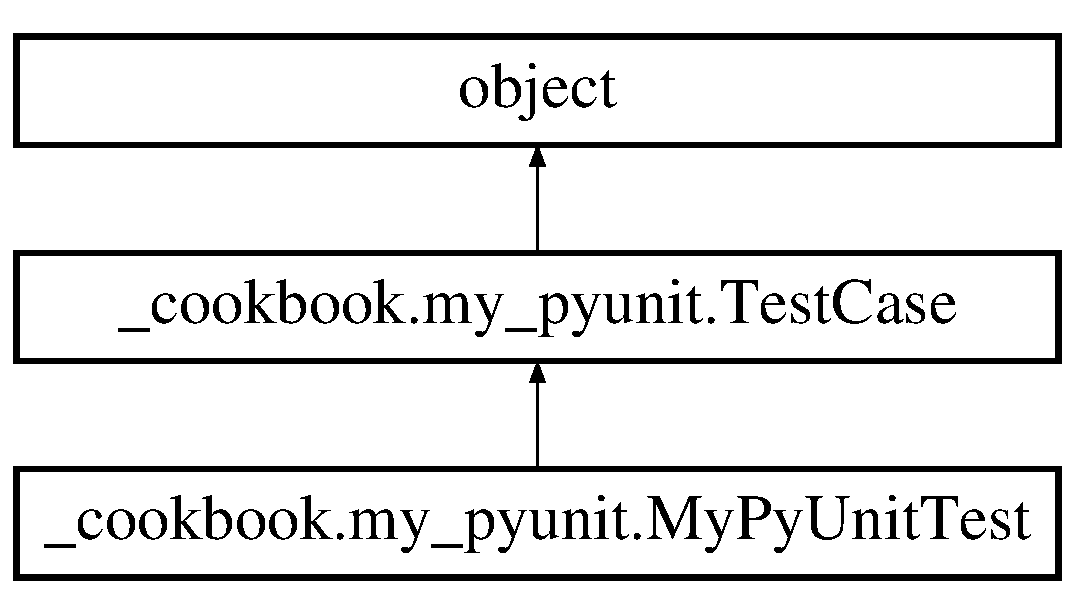
\includegraphics[height=3.000000cm]{d3/da6/class__cookbook_1_1my__pyunit_1_1MyPyUnitTest}
\end{center}
\end{figure}
\subsection*{Public Member Functions}
\begin{DoxyCompactItemize}
\item 
def \hyperlink{class__cookbook_1_1my__pyunit_1_1MyPyUnitTest_add8dae62bfa75940c16e29fe9e747ecf}{set\-Up}
\item 
def \hyperlink{class__cookbook_1_1my__pyunit_1_1MyPyUnitTest_a890394ba6f3a2be8fe549c77b48da1eb}{test\-\_\-a}
\item 
def \hyperlink{class__cookbook_1_1my__pyunit_1_1MyPyUnitTest_a782ad061affa65cc89b21fd95dc2d5d3}{test\-\_\-b}
\item 
def \hyperlink{class__cookbook_1_1my__pyunit_1_1MyPyUnitTest_a2cb2670508498a9de67fc530e752e3e4}{test\-\_\-c}
\item 
def \hyperlink{class__cookbook_1_1my__pyunit_1_1MyPyUnitTest_ab94bffe052b68b226914ef239b1658cb}{test\-\_\-d}
\item 
def \hyperlink{class__cookbook_1_1my__pyunit_1_1MyPyUnitTest_ae13b7160c2d4256fffe2b0846fbae5fc}{test\-\_\-e}
\item 
def \hyperlink{class__cookbook_1_1my__pyunit_1_1MyPyUnitTest_abdb32ee5c2e0a7fe9270c15f342046d0}{test\-\_\-f}
\item 
def \hyperlink{class__cookbook_1_1my__pyunit_1_1MyPyUnitTest_a350b8aa615b1ecb52ffceb3903a59f95}{test\-\_\-g}
\item 
def \hyperlink{class__cookbook_1_1my__pyunit_1_1MyPyUnitTest_ac72898ca445c2acee9cd93617ad38c5d}{test\-\_\-h}
\item 
def \hyperlink{class__cookbook_1_1my__pyunit_1_1MyPyUnitTest_ac619cd6aad71de2c754f72e62eb406f8}{test\-\_\-i}
\item 
def \hyperlink{class__cookbook_1_1my__pyunit_1_1MyPyUnitTest_a6f4660c020fbc79e44dc8937d9fc0cda}{test\-\_\-j}
\item 
def \hyperlink{class__cookbook_1_1my__pyunit_1_1MyPyUnitTest_a89c469ab6224a23625b9715b3f8abc0c}{test\-\_\-k}
\item 
def \hyperlink{class__cookbook_1_1my__pyunit_1_1MyPyUnitTest_a9dd83fe6d0e075ff1603828e076b5304}{test\-\_\-l}
\item 
def \hyperlink{class__cookbook_1_1my__pyunit_1_1MyPyUnitTest_a40bc1a1908b38c6656b6ad661b3ef0f9}{test\-\_\-m}
\item 
def \hyperlink{class__cookbook_1_1my__pyunit_1_1MyPyUnitTest_a3a1ef8a651622248b0b151ca0002e58d}{test\-\_\-n}
\item 
def \hyperlink{class__cookbook_1_1my__pyunit_1_1MyPyUnitTest_adb3aaee1a918b937ae6d40f3cb409951}{test\-\_\-o}
\item 
def \hyperlink{class__cookbook_1_1my__pyunit_1_1MyPyUnitTest_a6e1c88bb54ae00446aab3fb251920a3b}{test\-\_\-p}
\item 
def \hyperlink{class__cookbook_1_1my__pyunit_1_1MyPyUnitTest_a5d33a9a08e5c80403dc4e3762b4d198d}{test\-\_\-q}
\end{DoxyCompactItemize}
\subsection*{Additional Inherited Members}


\subsection{Detailed Description}
\begin{DoxyVerb}Test MyPyUnit\end{DoxyVerb}
 

Definition at line 226 of file my\-\_\-pyunit.\-py.



\subsection{Member Function Documentation}
\hypertarget{class__cookbook_1_1my__pyunit_1_1MyPyUnitTest_add8dae62bfa75940c16e29fe9e747ecf}{\index{\-\_\-cookbook\-::my\-\_\-pyunit\-::\-My\-Py\-Unit\-Test@{\-\_\-cookbook\-::my\-\_\-pyunit\-::\-My\-Py\-Unit\-Test}!set\-Up@{set\-Up}}
\index{set\-Up@{set\-Up}!_cookbook::my_pyunit::MyPyUnitTest@{\-\_\-cookbook\-::my\-\_\-pyunit\-::\-My\-Py\-Unit\-Test}}
\subsubsection[{set\-Up}]{\setlength{\rightskip}{0pt plus 5cm}def \-\_\-cookbook.\-my\-\_\-pyunit.\-My\-Py\-Unit\-Test.\-set\-Up (
\begin{DoxyParamCaption}
\item[{}]{self}
\end{DoxyParamCaption}
)}}\label{class__cookbook_1_1my__pyunit_1_1MyPyUnitTest_add8dae62bfa75940c16e29fe9e747ecf}


Definition at line 229 of file my\-\_\-pyunit.\-py.

\hypertarget{class__cookbook_1_1my__pyunit_1_1MyPyUnitTest_a890394ba6f3a2be8fe549c77b48da1eb}{\index{\-\_\-cookbook\-::my\-\_\-pyunit\-::\-My\-Py\-Unit\-Test@{\-\_\-cookbook\-::my\-\_\-pyunit\-::\-My\-Py\-Unit\-Test}!test\-\_\-a@{test\-\_\-a}}
\index{test\-\_\-a@{test\-\_\-a}!_cookbook::my_pyunit::MyPyUnitTest@{\-\_\-cookbook\-::my\-\_\-pyunit\-::\-My\-Py\-Unit\-Test}}
\subsubsection[{test\-\_\-a}]{\setlength{\rightskip}{0pt plus 5cm}def \-\_\-cookbook.\-my\-\_\-pyunit.\-My\-Py\-Unit\-Test.\-test\-\_\-a (
\begin{DoxyParamCaption}
\item[{}]{self}
\end{DoxyParamCaption}
)}}\label{class__cookbook_1_1my__pyunit_1_1MyPyUnitTest_a890394ba6f3a2be8fe549c77b48da1eb}


Definition at line 233 of file my\-\_\-pyunit.\-py.

\hypertarget{class__cookbook_1_1my__pyunit_1_1MyPyUnitTest_a782ad061affa65cc89b21fd95dc2d5d3}{\index{\-\_\-cookbook\-::my\-\_\-pyunit\-::\-My\-Py\-Unit\-Test@{\-\_\-cookbook\-::my\-\_\-pyunit\-::\-My\-Py\-Unit\-Test}!test\-\_\-b@{test\-\_\-b}}
\index{test\-\_\-b@{test\-\_\-b}!_cookbook::my_pyunit::MyPyUnitTest@{\-\_\-cookbook\-::my\-\_\-pyunit\-::\-My\-Py\-Unit\-Test}}
\subsubsection[{test\-\_\-b}]{\setlength{\rightskip}{0pt plus 5cm}def \-\_\-cookbook.\-my\-\_\-pyunit.\-My\-Py\-Unit\-Test.\-test\-\_\-b (
\begin{DoxyParamCaption}
\item[{}]{self}
\end{DoxyParamCaption}
)}}\label{class__cookbook_1_1my__pyunit_1_1MyPyUnitTest_a782ad061affa65cc89b21fd95dc2d5d3}


Definition at line 237 of file my\-\_\-pyunit.\-py.

\hypertarget{class__cookbook_1_1my__pyunit_1_1MyPyUnitTest_a2cb2670508498a9de67fc530e752e3e4}{\index{\-\_\-cookbook\-::my\-\_\-pyunit\-::\-My\-Py\-Unit\-Test@{\-\_\-cookbook\-::my\-\_\-pyunit\-::\-My\-Py\-Unit\-Test}!test\-\_\-c@{test\-\_\-c}}
\index{test\-\_\-c@{test\-\_\-c}!_cookbook::my_pyunit::MyPyUnitTest@{\-\_\-cookbook\-::my\-\_\-pyunit\-::\-My\-Py\-Unit\-Test}}
\subsubsection[{test\-\_\-c}]{\setlength{\rightskip}{0pt plus 5cm}def \-\_\-cookbook.\-my\-\_\-pyunit.\-My\-Py\-Unit\-Test.\-test\-\_\-c (
\begin{DoxyParamCaption}
\item[{}]{self}
\end{DoxyParamCaption}
)}}\label{class__cookbook_1_1my__pyunit_1_1MyPyUnitTest_a2cb2670508498a9de67fc530e752e3e4}


Definition at line 242 of file my\-\_\-pyunit.\-py.

\hypertarget{class__cookbook_1_1my__pyunit_1_1MyPyUnitTest_ab94bffe052b68b226914ef239b1658cb}{\index{\-\_\-cookbook\-::my\-\_\-pyunit\-::\-My\-Py\-Unit\-Test@{\-\_\-cookbook\-::my\-\_\-pyunit\-::\-My\-Py\-Unit\-Test}!test\-\_\-d@{test\-\_\-d}}
\index{test\-\_\-d@{test\-\_\-d}!_cookbook::my_pyunit::MyPyUnitTest@{\-\_\-cookbook\-::my\-\_\-pyunit\-::\-My\-Py\-Unit\-Test}}
\subsubsection[{test\-\_\-d}]{\setlength{\rightskip}{0pt plus 5cm}def \-\_\-cookbook.\-my\-\_\-pyunit.\-My\-Py\-Unit\-Test.\-test\-\_\-d (
\begin{DoxyParamCaption}
\item[{}]{self}
\end{DoxyParamCaption}
)}}\label{class__cookbook_1_1my__pyunit_1_1MyPyUnitTest_ab94bffe052b68b226914ef239b1658cb}


Definition at line 247 of file my\-\_\-pyunit.\-py.

\hypertarget{class__cookbook_1_1my__pyunit_1_1MyPyUnitTest_ae13b7160c2d4256fffe2b0846fbae5fc}{\index{\-\_\-cookbook\-::my\-\_\-pyunit\-::\-My\-Py\-Unit\-Test@{\-\_\-cookbook\-::my\-\_\-pyunit\-::\-My\-Py\-Unit\-Test}!test\-\_\-e@{test\-\_\-e}}
\index{test\-\_\-e@{test\-\_\-e}!_cookbook::my_pyunit::MyPyUnitTest@{\-\_\-cookbook\-::my\-\_\-pyunit\-::\-My\-Py\-Unit\-Test}}
\subsubsection[{test\-\_\-e}]{\setlength{\rightskip}{0pt plus 5cm}def \-\_\-cookbook.\-my\-\_\-pyunit.\-My\-Py\-Unit\-Test.\-test\-\_\-e (
\begin{DoxyParamCaption}
\item[{}]{self}
\end{DoxyParamCaption}
)}}\label{class__cookbook_1_1my__pyunit_1_1MyPyUnitTest_ae13b7160c2d4256fffe2b0846fbae5fc}


Definition at line 252 of file my\-\_\-pyunit.\-py.

\hypertarget{class__cookbook_1_1my__pyunit_1_1MyPyUnitTest_abdb32ee5c2e0a7fe9270c15f342046d0}{\index{\-\_\-cookbook\-::my\-\_\-pyunit\-::\-My\-Py\-Unit\-Test@{\-\_\-cookbook\-::my\-\_\-pyunit\-::\-My\-Py\-Unit\-Test}!test\-\_\-f@{test\-\_\-f}}
\index{test\-\_\-f@{test\-\_\-f}!_cookbook::my_pyunit::MyPyUnitTest@{\-\_\-cookbook\-::my\-\_\-pyunit\-::\-My\-Py\-Unit\-Test}}
\subsubsection[{test\-\_\-f}]{\setlength{\rightskip}{0pt plus 5cm}def \-\_\-cookbook.\-my\-\_\-pyunit.\-My\-Py\-Unit\-Test.\-test\-\_\-f (
\begin{DoxyParamCaption}
\item[{}]{self}
\end{DoxyParamCaption}
)}}\label{class__cookbook_1_1my__pyunit_1_1MyPyUnitTest_abdb32ee5c2e0a7fe9270c15f342046d0}


Definition at line 257 of file my\-\_\-pyunit.\-py.

\hypertarget{class__cookbook_1_1my__pyunit_1_1MyPyUnitTest_a350b8aa615b1ecb52ffceb3903a59f95}{\index{\-\_\-cookbook\-::my\-\_\-pyunit\-::\-My\-Py\-Unit\-Test@{\-\_\-cookbook\-::my\-\_\-pyunit\-::\-My\-Py\-Unit\-Test}!test\-\_\-g@{test\-\_\-g}}
\index{test\-\_\-g@{test\-\_\-g}!_cookbook::my_pyunit::MyPyUnitTest@{\-\_\-cookbook\-::my\-\_\-pyunit\-::\-My\-Py\-Unit\-Test}}
\subsubsection[{test\-\_\-g}]{\setlength{\rightskip}{0pt plus 5cm}def \-\_\-cookbook.\-my\-\_\-pyunit.\-My\-Py\-Unit\-Test.\-test\-\_\-g (
\begin{DoxyParamCaption}
\item[{}]{self}
\end{DoxyParamCaption}
)}}\label{class__cookbook_1_1my__pyunit_1_1MyPyUnitTest_a350b8aa615b1ecb52ffceb3903a59f95}


Definition at line 262 of file my\-\_\-pyunit.\-py.

\hypertarget{class__cookbook_1_1my__pyunit_1_1MyPyUnitTest_ac72898ca445c2acee9cd93617ad38c5d}{\index{\-\_\-cookbook\-::my\-\_\-pyunit\-::\-My\-Py\-Unit\-Test@{\-\_\-cookbook\-::my\-\_\-pyunit\-::\-My\-Py\-Unit\-Test}!test\-\_\-h@{test\-\_\-h}}
\index{test\-\_\-h@{test\-\_\-h}!_cookbook::my_pyunit::MyPyUnitTest@{\-\_\-cookbook\-::my\-\_\-pyunit\-::\-My\-Py\-Unit\-Test}}
\subsubsection[{test\-\_\-h}]{\setlength{\rightskip}{0pt plus 5cm}def \-\_\-cookbook.\-my\-\_\-pyunit.\-My\-Py\-Unit\-Test.\-test\-\_\-h (
\begin{DoxyParamCaption}
\item[{}]{self}
\end{DoxyParamCaption}
)}}\label{class__cookbook_1_1my__pyunit_1_1MyPyUnitTest_ac72898ca445c2acee9cd93617ad38c5d}


Definition at line 267 of file my\-\_\-pyunit.\-py.

\hypertarget{class__cookbook_1_1my__pyunit_1_1MyPyUnitTest_ac619cd6aad71de2c754f72e62eb406f8}{\index{\-\_\-cookbook\-::my\-\_\-pyunit\-::\-My\-Py\-Unit\-Test@{\-\_\-cookbook\-::my\-\_\-pyunit\-::\-My\-Py\-Unit\-Test}!test\-\_\-i@{test\-\_\-i}}
\index{test\-\_\-i@{test\-\_\-i}!_cookbook::my_pyunit::MyPyUnitTest@{\-\_\-cookbook\-::my\-\_\-pyunit\-::\-My\-Py\-Unit\-Test}}
\subsubsection[{test\-\_\-i}]{\setlength{\rightskip}{0pt plus 5cm}def \-\_\-cookbook.\-my\-\_\-pyunit.\-My\-Py\-Unit\-Test.\-test\-\_\-i (
\begin{DoxyParamCaption}
\item[{}]{self}
\end{DoxyParamCaption}
)}}\label{class__cookbook_1_1my__pyunit_1_1MyPyUnitTest_ac619cd6aad71de2c754f72e62eb406f8}


Definition at line 272 of file my\-\_\-pyunit.\-py.

\hypertarget{class__cookbook_1_1my__pyunit_1_1MyPyUnitTest_a6f4660c020fbc79e44dc8937d9fc0cda}{\index{\-\_\-cookbook\-::my\-\_\-pyunit\-::\-My\-Py\-Unit\-Test@{\-\_\-cookbook\-::my\-\_\-pyunit\-::\-My\-Py\-Unit\-Test}!test\-\_\-j@{test\-\_\-j}}
\index{test\-\_\-j@{test\-\_\-j}!_cookbook::my_pyunit::MyPyUnitTest@{\-\_\-cookbook\-::my\-\_\-pyunit\-::\-My\-Py\-Unit\-Test}}
\subsubsection[{test\-\_\-j}]{\setlength{\rightskip}{0pt plus 5cm}def \-\_\-cookbook.\-my\-\_\-pyunit.\-My\-Py\-Unit\-Test.\-test\-\_\-j (
\begin{DoxyParamCaption}
\item[{}]{self}
\end{DoxyParamCaption}
)}}\label{class__cookbook_1_1my__pyunit_1_1MyPyUnitTest_a6f4660c020fbc79e44dc8937d9fc0cda}


Definition at line 277 of file my\-\_\-pyunit.\-py.

\hypertarget{class__cookbook_1_1my__pyunit_1_1MyPyUnitTest_a89c469ab6224a23625b9715b3f8abc0c}{\index{\-\_\-cookbook\-::my\-\_\-pyunit\-::\-My\-Py\-Unit\-Test@{\-\_\-cookbook\-::my\-\_\-pyunit\-::\-My\-Py\-Unit\-Test}!test\-\_\-k@{test\-\_\-k}}
\index{test\-\_\-k@{test\-\_\-k}!_cookbook::my_pyunit::MyPyUnitTest@{\-\_\-cookbook\-::my\-\_\-pyunit\-::\-My\-Py\-Unit\-Test}}
\subsubsection[{test\-\_\-k}]{\setlength{\rightskip}{0pt plus 5cm}def \-\_\-cookbook.\-my\-\_\-pyunit.\-My\-Py\-Unit\-Test.\-test\-\_\-k (
\begin{DoxyParamCaption}
\item[{}]{self}
\end{DoxyParamCaption}
)}}\label{class__cookbook_1_1my__pyunit_1_1MyPyUnitTest_a89c469ab6224a23625b9715b3f8abc0c}


Definition at line 282 of file my\-\_\-pyunit.\-py.

\hypertarget{class__cookbook_1_1my__pyunit_1_1MyPyUnitTest_a9dd83fe6d0e075ff1603828e076b5304}{\index{\-\_\-cookbook\-::my\-\_\-pyunit\-::\-My\-Py\-Unit\-Test@{\-\_\-cookbook\-::my\-\_\-pyunit\-::\-My\-Py\-Unit\-Test}!test\-\_\-l@{test\-\_\-l}}
\index{test\-\_\-l@{test\-\_\-l}!_cookbook::my_pyunit::MyPyUnitTest@{\-\_\-cookbook\-::my\-\_\-pyunit\-::\-My\-Py\-Unit\-Test}}
\subsubsection[{test\-\_\-l}]{\setlength{\rightskip}{0pt plus 5cm}def \-\_\-cookbook.\-my\-\_\-pyunit.\-My\-Py\-Unit\-Test.\-test\-\_\-l (
\begin{DoxyParamCaption}
\item[{}]{self}
\end{DoxyParamCaption}
)}}\label{class__cookbook_1_1my__pyunit_1_1MyPyUnitTest_a9dd83fe6d0e075ff1603828e076b5304}


Definition at line 287 of file my\-\_\-pyunit.\-py.

\hypertarget{class__cookbook_1_1my__pyunit_1_1MyPyUnitTest_a40bc1a1908b38c6656b6ad661b3ef0f9}{\index{\-\_\-cookbook\-::my\-\_\-pyunit\-::\-My\-Py\-Unit\-Test@{\-\_\-cookbook\-::my\-\_\-pyunit\-::\-My\-Py\-Unit\-Test}!test\-\_\-m@{test\-\_\-m}}
\index{test\-\_\-m@{test\-\_\-m}!_cookbook::my_pyunit::MyPyUnitTest@{\-\_\-cookbook\-::my\-\_\-pyunit\-::\-My\-Py\-Unit\-Test}}
\subsubsection[{test\-\_\-m}]{\setlength{\rightskip}{0pt plus 5cm}def \-\_\-cookbook.\-my\-\_\-pyunit.\-My\-Py\-Unit\-Test.\-test\-\_\-m (
\begin{DoxyParamCaption}
\item[{}]{self}
\end{DoxyParamCaption}
)}}\label{class__cookbook_1_1my__pyunit_1_1MyPyUnitTest_a40bc1a1908b38c6656b6ad661b3ef0f9}


Definition at line 292 of file my\-\_\-pyunit.\-py.

\hypertarget{class__cookbook_1_1my__pyunit_1_1MyPyUnitTest_a3a1ef8a651622248b0b151ca0002e58d}{\index{\-\_\-cookbook\-::my\-\_\-pyunit\-::\-My\-Py\-Unit\-Test@{\-\_\-cookbook\-::my\-\_\-pyunit\-::\-My\-Py\-Unit\-Test}!test\-\_\-n@{test\-\_\-n}}
\index{test\-\_\-n@{test\-\_\-n}!_cookbook::my_pyunit::MyPyUnitTest@{\-\_\-cookbook\-::my\-\_\-pyunit\-::\-My\-Py\-Unit\-Test}}
\subsubsection[{test\-\_\-n}]{\setlength{\rightskip}{0pt plus 5cm}def \-\_\-cookbook.\-my\-\_\-pyunit.\-My\-Py\-Unit\-Test.\-test\-\_\-n (
\begin{DoxyParamCaption}
\item[{}]{self}
\end{DoxyParamCaption}
)}}\label{class__cookbook_1_1my__pyunit_1_1MyPyUnitTest_a3a1ef8a651622248b0b151ca0002e58d}


Definition at line 297 of file my\-\_\-pyunit.\-py.

\hypertarget{class__cookbook_1_1my__pyunit_1_1MyPyUnitTest_adb3aaee1a918b937ae6d40f3cb409951}{\index{\-\_\-cookbook\-::my\-\_\-pyunit\-::\-My\-Py\-Unit\-Test@{\-\_\-cookbook\-::my\-\_\-pyunit\-::\-My\-Py\-Unit\-Test}!test\-\_\-o@{test\-\_\-o}}
\index{test\-\_\-o@{test\-\_\-o}!_cookbook::my_pyunit::MyPyUnitTest@{\-\_\-cookbook\-::my\-\_\-pyunit\-::\-My\-Py\-Unit\-Test}}
\subsubsection[{test\-\_\-o}]{\setlength{\rightskip}{0pt plus 5cm}def \-\_\-cookbook.\-my\-\_\-pyunit.\-My\-Py\-Unit\-Test.\-test\-\_\-o (
\begin{DoxyParamCaption}
\item[{}]{self}
\end{DoxyParamCaption}
)}}\label{class__cookbook_1_1my__pyunit_1_1MyPyUnitTest_adb3aaee1a918b937ae6d40f3cb409951}


Definition at line 302 of file my\-\_\-pyunit.\-py.

\hypertarget{class__cookbook_1_1my__pyunit_1_1MyPyUnitTest_a6e1c88bb54ae00446aab3fb251920a3b}{\index{\-\_\-cookbook\-::my\-\_\-pyunit\-::\-My\-Py\-Unit\-Test@{\-\_\-cookbook\-::my\-\_\-pyunit\-::\-My\-Py\-Unit\-Test}!test\-\_\-p@{test\-\_\-p}}
\index{test\-\_\-p@{test\-\_\-p}!_cookbook::my_pyunit::MyPyUnitTest@{\-\_\-cookbook\-::my\-\_\-pyunit\-::\-My\-Py\-Unit\-Test}}
\subsubsection[{test\-\_\-p}]{\setlength{\rightskip}{0pt plus 5cm}def \-\_\-cookbook.\-my\-\_\-pyunit.\-My\-Py\-Unit\-Test.\-test\-\_\-p (
\begin{DoxyParamCaption}
\item[{}]{self}
\end{DoxyParamCaption}
)}}\label{class__cookbook_1_1my__pyunit_1_1MyPyUnitTest_a6e1c88bb54ae00446aab3fb251920a3b}


Definition at line 307 of file my\-\_\-pyunit.\-py.

\hypertarget{class__cookbook_1_1my__pyunit_1_1MyPyUnitTest_a5d33a9a08e5c80403dc4e3762b4d198d}{\index{\-\_\-cookbook\-::my\-\_\-pyunit\-::\-My\-Py\-Unit\-Test@{\-\_\-cookbook\-::my\-\_\-pyunit\-::\-My\-Py\-Unit\-Test}!test\-\_\-q@{test\-\_\-q}}
\index{test\-\_\-q@{test\-\_\-q}!_cookbook::my_pyunit::MyPyUnitTest@{\-\_\-cookbook\-::my\-\_\-pyunit\-::\-My\-Py\-Unit\-Test}}
\subsubsection[{test\-\_\-q}]{\setlength{\rightskip}{0pt plus 5cm}def \-\_\-cookbook.\-my\-\_\-pyunit.\-My\-Py\-Unit\-Test.\-test\-\_\-q (
\begin{DoxyParamCaption}
\item[{}]{self}
\end{DoxyParamCaption}
)}}\label{class__cookbook_1_1my__pyunit_1_1MyPyUnitTest_a5d33a9a08e5c80403dc4e3762b4d198d}


Definition at line 312 of file my\-\_\-pyunit.\-py.



The documentation for this class was generated from the following file\-:\begin{DoxyCompactItemize}
\item 
\-\_\-cookbook/\hyperlink{my__pyunit_8py}{my\-\_\-pyunit.\-py}\end{DoxyCompactItemize}

\hypertarget{class__cookbook_1_1thread_1_1my__queue_1_1MyQueue}{\section{\-\_\-cookbook.\-thread.\-my\-\_\-queue.\-My\-Queue Class Reference}
\label{class__cookbook_1_1thread_1_1my__queue_1_1MyQueue}\index{\-\_\-cookbook.\-thread.\-my\-\_\-queue.\-My\-Queue@{\-\_\-cookbook.\-thread.\-my\-\_\-queue.\-My\-Queue}}
}
Inheritance diagram for \-\_\-cookbook.\-thread.\-my\-\_\-queue.\-My\-Queue\-:\begin{figure}[H]
\begin{center}
\leavevmode
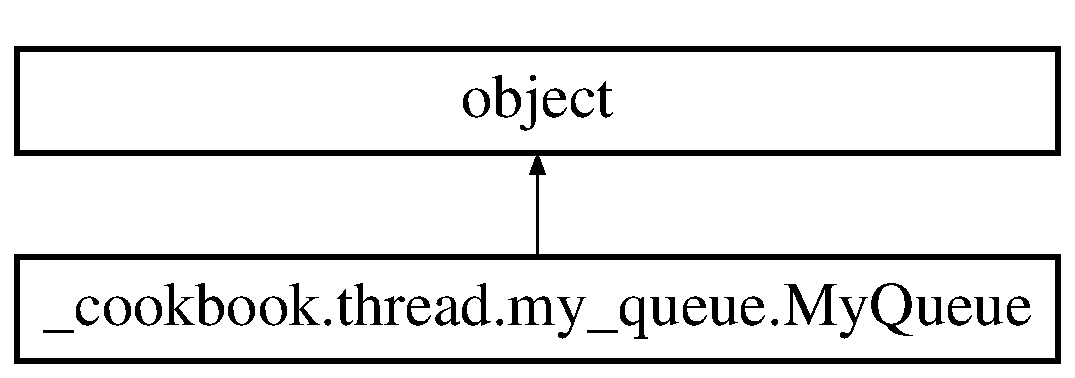
\includegraphics[height=2.000000cm]{d6/dcc/class__cookbook_1_1thread_1_1my__queue_1_1MyQueue}
\end{center}
\end{figure}
\subsection*{Public Member Functions}
\begin{DoxyCompactItemize}
\item 
def \hyperlink{class__cookbook_1_1thread_1_1my__queue_1_1MyQueue_a6f9f8590a70aca88737939c2e793b854}{\-\_\-\-\_\-init\-\_\-\-\_\-}
\item 
def \hyperlink{class__cookbook_1_1thread_1_1my__queue_1_1MyQueue_a628dba4427a33d27eecd3fbfc7c2366d}{qsize}
\item 
def \hyperlink{class__cookbook_1_1thread_1_1my__queue_1_1MyQueue_a80d8c2b5b61df971805ad4aad520c622}{empty}
\item 
def \hyperlink{class__cookbook_1_1thread_1_1my__queue_1_1MyQueue_ab34edaaa1bcc947dfc10ccaffddfd9ef}{full}
\item 
def \hyperlink{class__cookbook_1_1thread_1_1my__queue_1_1MyQueue_addb2a52a6b08211ecd10ffee6614f55e}{task\-\_\-done}
\item 
def \hyperlink{class__cookbook_1_1thread_1_1my__queue_1_1MyQueue_a9b25ef168e9200c7091c6bb1faf0ad84}{join}
\item 
def \hyperlink{class__cookbook_1_1thread_1_1my__queue_1_1MyQueue_abb8937cad32dd7fb7d5c6a7f77041e9b}{get}
\item 
def \hyperlink{class__cookbook_1_1thread_1_1my__queue_1_1MyQueue_adac4ae837b6ef2f9150741a9e2cd23b6}{put}
\end{DoxyCompactItemize}
\subsection*{Private Member Functions}
\begin{DoxyCompactItemize}
\item 
def \hyperlink{class__cookbook_1_1thread_1_1my__queue_1_1MyQueue_ab654b5e36b4cc4d199360fda3c45e5cb}{\-\_\-init\-\_\-queue}
\item 
def \hyperlink{class__cookbook_1_1thread_1_1my__queue_1_1MyQueue_a916e03faf976d1f2e5ca1eb144bd260f}{\-\_\-queue\-\_\-size}
\item 
def \hyperlink{class__cookbook_1_1thread_1_1my__queue_1_1MyQueue_a3900db1ad5d80f30c0af8f96b36794c2}{\-\_\-put}
\item 
def \hyperlink{class__cookbook_1_1thread_1_1my__queue_1_1MyQueue_a44dbd36a7138e556841b7e37f71d2f6d}{\-\_\-get}
\end{DoxyCompactItemize}
\subsection*{Private Attributes}
\begin{DoxyCompactItemize}
\item 
\hyperlink{class__cookbook_1_1thread_1_1my__queue_1_1MyQueue_a60146b776c7697f2c44a7def52f96add}{\-\_\-maxsize}
\item 
\hyperlink{class__cookbook_1_1thread_1_1my__queue_1_1MyQueue_a89d49165c60fbe8c6f3b95ee39af48fd}{\-\_\-lock}
\item 
\hyperlink{class__cookbook_1_1thread_1_1my__queue_1_1MyQueue_af25788e43ddebdb88598336257767d7e}{\-\_\-cond\-\_\-not\-\_\-empty}
\item 
\hyperlink{class__cookbook_1_1thread_1_1my__queue_1_1MyQueue_a35b085cc547625cb027ce8389214eedb}{\-\_\-cond\-\_\-not\-\_\-full}
\item 
\hyperlink{class__cookbook_1_1thread_1_1my__queue_1_1MyQueue_a39fe4c64fec0ccaf6c01063fe1c4d2dd}{\-\_\-cond\-\_\-all\-\_\-tasks\-\_\-done}
\item 
\hyperlink{class__cookbook_1_1thread_1_1my__queue_1_1MyQueue_a7ba895923806b0797c84dedb2eb6bbf9}{\-\_\-unfinished\-\_\-tasks}
\item 
\hyperlink{class__cookbook_1_1thread_1_1my__queue_1_1MyQueue_ab96b072fd4230d0ba12b280cc302996a}{\-\_\-queue}
\end{DoxyCompactItemize}


\subsection{Detailed Description}
\begin{DoxyVerb}A class whose instances are multi-producer, multi-cusumer queues.\end{DoxyVerb}
 

Definition at line 76 of file my\-\_\-queue.\-py.



\subsection{Constructor \& Destructor Documentation}
\hypertarget{class__cookbook_1_1thread_1_1my__queue_1_1MyQueue_a6f9f8590a70aca88737939c2e793b854}{\index{\-\_\-cookbook\-::thread\-::my\-\_\-queue\-::\-My\-Queue@{\-\_\-cookbook\-::thread\-::my\-\_\-queue\-::\-My\-Queue}!\-\_\-\-\_\-init\-\_\-\-\_\-@{\-\_\-\-\_\-init\-\_\-\-\_\-}}
\index{\-\_\-\-\_\-init\-\_\-\-\_\-@{\-\_\-\-\_\-init\-\_\-\-\_\-}!_cookbook::thread::my_queue::MyQueue@{\-\_\-cookbook\-::thread\-::my\-\_\-queue\-::\-My\-Queue}}
\subsubsection[{\-\_\-\-\_\-init\-\_\-\-\_\-}]{\setlength{\rightskip}{0pt plus 5cm}def \-\_\-cookbook.\-thread.\-my\-\_\-queue.\-My\-Queue.\-\_\-\-\_\-init\-\_\-\-\_\- (
\begin{DoxyParamCaption}
\item[{}]{self, }
\item[{}]{maxsize = {\ttfamily 0}}
\end{DoxyParamCaption}
)}}\label{class__cookbook_1_1thread_1_1my__queue_1_1MyQueue_a6f9f8590a70aca88737939c2e793b854}


Definition at line 79 of file my\-\_\-queue.\-py.



\subsection{Member Function Documentation}
\hypertarget{class__cookbook_1_1thread_1_1my__queue_1_1MyQueue_a44dbd36a7138e556841b7e37f71d2f6d}{\index{\-\_\-cookbook\-::thread\-::my\-\_\-queue\-::\-My\-Queue@{\-\_\-cookbook\-::thread\-::my\-\_\-queue\-::\-My\-Queue}!\-\_\-get@{\-\_\-get}}
\index{\-\_\-get@{\-\_\-get}!_cookbook::thread::my_queue::MyQueue@{\-\_\-cookbook\-::thread\-::my\-\_\-queue\-::\-My\-Queue}}
\subsubsection[{\-\_\-get}]{\setlength{\rightskip}{0pt plus 5cm}def \-\_\-cookbook.\-thread.\-my\-\_\-queue.\-My\-Queue.\-\_\-get (
\begin{DoxyParamCaption}
\item[{}]{self}
\end{DoxyParamCaption}
)\hspace{0.3cm}{\ttfamily [private]}}}\label{class__cookbook_1_1thread_1_1my__queue_1_1MyQueue_a44dbd36a7138e556841b7e37f71d2f6d}
\begin{DoxyVerb}Get an item from a queue.\end{DoxyVerb}
 

Definition at line 183 of file my\-\_\-queue.\-py.

\hypertarget{class__cookbook_1_1thread_1_1my__queue_1_1MyQueue_ab654b5e36b4cc4d199360fda3c45e5cb}{\index{\-\_\-cookbook\-::thread\-::my\-\_\-queue\-::\-My\-Queue@{\-\_\-cookbook\-::thread\-::my\-\_\-queue\-::\-My\-Queue}!\-\_\-init\-\_\-queue@{\-\_\-init\-\_\-queue}}
\index{\-\_\-init\-\_\-queue@{\-\_\-init\-\_\-queue}!_cookbook::thread::my_queue::MyQueue@{\-\_\-cookbook\-::thread\-::my\-\_\-queue\-::\-My\-Queue}}
\subsubsection[{\-\_\-init\-\_\-queue}]{\setlength{\rightskip}{0pt plus 5cm}def \-\_\-cookbook.\-thread.\-my\-\_\-queue.\-My\-Queue.\-\_\-init\-\_\-queue (
\begin{DoxyParamCaption}
\item[{}]{self, }
\item[{}]{maxsize}
\end{DoxyParamCaption}
)\hspace{0.3cm}{\ttfamily [private]}}}\label{class__cookbook_1_1thread_1_1my__queue_1_1MyQueue_ab654b5e36b4cc4d199360fda3c45e5cb}
\begin{DoxyVerb}Initialize the queue representation.\end{DoxyVerb}
 

Definition at line 166 of file my\-\_\-queue.\-py.

\hypertarget{class__cookbook_1_1thread_1_1my__queue_1_1MyQueue_a3900db1ad5d80f30c0af8f96b36794c2}{\index{\-\_\-cookbook\-::thread\-::my\-\_\-queue\-::\-My\-Queue@{\-\_\-cookbook\-::thread\-::my\-\_\-queue\-::\-My\-Queue}!\-\_\-put@{\-\_\-put}}
\index{\-\_\-put@{\-\_\-put}!_cookbook::thread::my_queue::MyQueue@{\-\_\-cookbook\-::thread\-::my\-\_\-queue\-::\-My\-Queue}}
\subsubsection[{\-\_\-put}]{\setlength{\rightskip}{0pt plus 5cm}def \-\_\-cookbook.\-thread.\-my\-\_\-queue.\-My\-Queue.\-\_\-put (
\begin{DoxyParamCaption}
\item[{}]{self, }
\item[{}]{item}
\end{DoxyParamCaption}
)\hspace{0.3cm}{\ttfamily [private]}}}\label{class__cookbook_1_1thread_1_1my__queue_1_1MyQueue_a3900db1ad5d80f30c0af8f96b36794c2}
\begin{DoxyVerb}Put an item in the queue.\end{DoxyVerb}
 

Definition at line 178 of file my\-\_\-queue.\-py.

\hypertarget{class__cookbook_1_1thread_1_1my__queue_1_1MyQueue_a916e03faf976d1f2e5ca1eb144bd260f}{\index{\-\_\-cookbook\-::thread\-::my\-\_\-queue\-::\-My\-Queue@{\-\_\-cookbook\-::thread\-::my\-\_\-queue\-::\-My\-Queue}!\-\_\-queue\-\_\-size@{\-\_\-queue\-\_\-size}}
\index{\-\_\-queue\-\_\-size@{\-\_\-queue\-\_\-size}!_cookbook::thread::my_queue::MyQueue@{\-\_\-cookbook\-::thread\-::my\-\_\-queue\-::\-My\-Queue}}
\subsubsection[{\-\_\-queue\-\_\-size}]{\setlength{\rightskip}{0pt plus 5cm}def \-\_\-cookbook.\-thread.\-my\-\_\-queue.\-My\-Queue.\-\_\-queue\-\_\-size (
\begin{DoxyParamCaption}
\item[{}]{self}
\end{DoxyParamCaption}
)\hspace{0.3cm}{\ttfamily [private]}}}\label{class__cookbook_1_1thread_1_1my__queue_1_1MyQueue_a916e03faf976d1f2e5ca1eb144bd260f}


Definition at line 174 of file my\-\_\-queue.\-py.

\hypertarget{class__cookbook_1_1thread_1_1my__queue_1_1MyQueue_a80d8c2b5b61df971805ad4aad520c622}{\index{\-\_\-cookbook\-::thread\-::my\-\_\-queue\-::\-My\-Queue@{\-\_\-cookbook\-::thread\-::my\-\_\-queue\-::\-My\-Queue}!empty@{empty}}
\index{empty@{empty}!_cookbook::thread::my_queue::MyQueue@{\-\_\-cookbook\-::thread\-::my\-\_\-queue\-::\-My\-Queue}}
\subsubsection[{empty}]{\setlength{\rightskip}{0pt plus 5cm}def \-\_\-cookbook.\-thread.\-my\-\_\-queue.\-My\-Queue.\-empty (
\begin{DoxyParamCaption}
\item[{}]{self}
\end{DoxyParamCaption}
)}}\label{class__cookbook_1_1thread_1_1my__queue_1_1MyQueue_a80d8c2b5b61df971805ad4aad520c622}
\begin{DoxyVerb}Check if the queue is empty. (NOT reliable)\end{DoxyVerb}
 

Definition at line 105 of file my\-\_\-queue.\-py.

\hypertarget{class__cookbook_1_1thread_1_1my__queue_1_1MyQueue_ab34edaaa1bcc947dfc10ccaffddfd9ef}{\index{\-\_\-cookbook\-::thread\-::my\-\_\-queue\-::\-My\-Queue@{\-\_\-cookbook\-::thread\-::my\-\_\-queue\-::\-My\-Queue}!full@{full}}
\index{full@{full}!_cookbook::thread::my_queue::MyQueue@{\-\_\-cookbook\-::thread\-::my\-\_\-queue\-::\-My\-Queue}}
\subsubsection[{full}]{\setlength{\rightskip}{0pt plus 5cm}def \-\_\-cookbook.\-thread.\-my\-\_\-queue.\-My\-Queue.\-full (
\begin{DoxyParamCaption}
\item[{}]{self}
\end{DoxyParamCaption}
)}}\label{class__cookbook_1_1thread_1_1my__queue_1_1MyQueue_ab34edaaa1bcc947dfc10ccaffddfd9ef}
\begin{DoxyVerb}Check if the queue is full. (NOT reliable)\end{DoxyVerb}
 

Definition at line 111 of file my\-\_\-queue.\-py.

\hypertarget{class__cookbook_1_1thread_1_1my__queue_1_1MyQueue_abb8937cad32dd7fb7d5c6a7f77041e9b}{\index{\-\_\-cookbook\-::thread\-::my\-\_\-queue\-::\-My\-Queue@{\-\_\-cookbook\-::thread\-::my\-\_\-queue\-::\-My\-Queue}!get@{get}}
\index{get@{get}!_cookbook::thread::my_queue::MyQueue@{\-\_\-cookbook\-::thread\-::my\-\_\-queue\-::\-My\-Queue}}
\subsubsection[{get}]{\setlength{\rightskip}{0pt plus 5cm}def \-\_\-cookbook.\-thread.\-my\-\_\-queue.\-My\-Queue.\-get (
\begin{DoxyParamCaption}
\item[{}]{self}
\end{DoxyParamCaption}
)}}\label{class__cookbook_1_1thread_1_1my__queue_1_1MyQueue_abb8937cad32dd7fb7d5c6a7f77041e9b}
\begin{DoxyVerb}Get an item from the queue.\end{DoxyVerb}
 

Definition at line 144 of file my\-\_\-queue.\-py.

\hypertarget{class__cookbook_1_1thread_1_1my__queue_1_1MyQueue_a9b25ef168e9200c7091c6bb1faf0ad84}{\index{\-\_\-cookbook\-::thread\-::my\-\_\-queue\-::\-My\-Queue@{\-\_\-cookbook\-::thread\-::my\-\_\-queue\-::\-My\-Queue}!join@{join}}
\index{join@{join}!_cookbook::thread::my_queue::MyQueue@{\-\_\-cookbook\-::thread\-::my\-\_\-queue\-::\-My\-Queue}}
\subsubsection[{join}]{\setlength{\rightskip}{0pt plus 5cm}def \-\_\-cookbook.\-thread.\-my\-\_\-queue.\-My\-Queue.\-join (
\begin{DoxyParamCaption}
\item[{}]{self}
\end{DoxyParamCaption}
)}}\label{class__cookbook_1_1thread_1_1my__queue_1_1MyQueue_a9b25ef168e9200c7091c6bb1faf0ad84}
\begin{DoxyVerb}Block until all items in the queue have been processed.\end{DoxyVerb}
 

Definition at line 137 of file my\-\_\-queue.\-py.

\hypertarget{class__cookbook_1_1thread_1_1my__queue_1_1MyQueue_adac4ae837b6ef2f9150741a9e2cd23b6}{\index{\-\_\-cookbook\-::thread\-::my\-\_\-queue\-::\-My\-Queue@{\-\_\-cookbook\-::thread\-::my\-\_\-queue\-::\-My\-Queue}!put@{put}}
\index{put@{put}!_cookbook::thread::my_queue::MyQueue@{\-\_\-cookbook\-::thread\-::my\-\_\-queue\-::\-My\-Queue}}
\subsubsection[{put}]{\setlength{\rightskip}{0pt plus 5cm}def \-\_\-cookbook.\-thread.\-my\-\_\-queue.\-My\-Queue.\-put (
\begin{DoxyParamCaption}
\item[{}]{self, }
\item[{}]{item}
\end{DoxyParamCaption}
)}}\label{class__cookbook_1_1thread_1_1my__queue_1_1MyQueue_adac4ae837b6ef2f9150741a9e2cd23b6}
\begin{DoxyVerb}Put an item into the queue.\end{DoxyVerb}
 

Definition at line 154 of file my\-\_\-queue.\-py.

\hypertarget{class__cookbook_1_1thread_1_1my__queue_1_1MyQueue_a628dba4427a33d27eecd3fbfc7c2366d}{\index{\-\_\-cookbook\-::thread\-::my\-\_\-queue\-::\-My\-Queue@{\-\_\-cookbook\-::thread\-::my\-\_\-queue\-::\-My\-Queue}!qsize@{qsize}}
\index{qsize@{qsize}!_cookbook::thread::my_queue::MyQueue@{\-\_\-cookbook\-::thread\-::my\-\_\-queue\-::\-My\-Queue}}
\subsubsection[{qsize}]{\setlength{\rightskip}{0pt plus 5cm}def \-\_\-cookbook.\-thread.\-my\-\_\-queue.\-My\-Queue.\-qsize (
\begin{DoxyParamCaption}
\item[{}]{self}
\end{DoxyParamCaption}
)}}\label{class__cookbook_1_1thread_1_1my__queue_1_1MyQueue_a628dba4427a33d27eecd3fbfc7c2366d}
\begin{DoxyVerb}Return the queue actual size. (NOT reliable)\end{DoxyVerb}
 

Definition at line 99 of file my\-\_\-queue.\-py.

\hypertarget{class__cookbook_1_1thread_1_1my__queue_1_1MyQueue_addb2a52a6b08211ecd10ffee6614f55e}{\index{\-\_\-cookbook\-::thread\-::my\-\_\-queue\-::\-My\-Queue@{\-\_\-cookbook\-::thread\-::my\-\_\-queue\-::\-My\-Queue}!task\-\_\-done@{task\-\_\-done}}
\index{task\-\_\-done@{task\-\_\-done}!_cookbook::thread::my_queue::MyQueue@{\-\_\-cookbook\-::thread\-::my\-\_\-queue\-::\-My\-Queue}}
\subsubsection[{task\-\_\-done}]{\setlength{\rightskip}{0pt plus 5cm}def \-\_\-cookbook.\-thread.\-my\-\_\-queue.\-My\-Queue.\-task\-\_\-done (
\begin{DoxyParamCaption}
\item[{}]{self}
\end{DoxyParamCaption}
)}}\label{class__cookbook_1_1thread_1_1my__queue_1_1MyQueue_addb2a52a6b08211ecd10ffee6614f55e}
\begin{DoxyVerb}Indicate that a formerly enqueued task is finished.

Used by Queue cusumer threads,. For each `get()` used to fetch a task,
a subsequent call to `task_done()` tells that the processing on the
task is finished.

If a `join()` is currently blocking, it will resume when all items
have been processed.
\end{DoxyVerb}
 

Definition at line 118 of file my\-\_\-queue.\-py.



\subsection{Member Data Documentation}
\hypertarget{class__cookbook_1_1thread_1_1my__queue_1_1MyQueue_a39fe4c64fec0ccaf6c01063fe1c4d2dd}{\index{\-\_\-cookbook\-::thread\-::my\-\_\-queue\-::\-My\-Queue@{\-\_\-cookbook\-::thread\-::my\-\_\-queue\-::\-My\-Queue}!\-\_\-cond\-\_\-all\-\_\-tasks\-\_\-done@{\-\_\-cond\-\_\-all\-\_\-tasks\-\_\-done}}
\index{\-\_\-cond\-\_\-all\-\_\-tasks\-\_\-done@{\-\_\-cond\-\_\-all\-\_\-tasks\-\_\-done}!_cookbook::thread::my_queue::MyQueue@{\-\_\-cookbook\-::thread\-::my\-\_\-queue\-::\-My\-Queue}}
\subsubsection[{\-\_\-cond\-\_\-all\-\_\-tasks\-\_\-done}]{\setlength{\rightskip}{0pt plus 5cm}\-\_\-cookbook.\-thread.\-my\-\_\-queue.\-My\-Queue.\-\_\-cond\-\_\-all\-\_\-tasks\-\_\-done\hspace{0.3cm}{\ttfamily [private]}}}\label{class__cookbook_1_1thread_1_1my__queue_1_1MyQueue_a39fe4c64fec0ccaf6c01063fe1c4d2dd}


Definition at line 95 of file my\-\_\-queue.\-py.

\hypertarget{class__cookbook_1_1thread_1_1my__queue_1_1MyQueue_af25788e43ddebdb88598336257767d7e}{\index{\-\_\-cookbook\-::thread\-::my\-\_\-queue\-::\-My\-Queue@{\-\_\-cookbook\-::thread\-::my\-\_\-queue\-::\-My\-Queue}!\-\_\-cond\-\_\-not\-\_\-empty@{\-\_\-cond\-\_\-not\-\_\-empty}}
\index{\-\_\-cond\-\_\-not\-\_\-empty@{\-\_\-cond\-\_\-not\-\_\-empty}!_cookbook::thread::my_queue::MyQueue@{\-\_\-cookbook\-::thread\-::my\-\_\-queue\-::\-My\-Queue}}
\subsubsection[{\-\_\-cond\-\_\-not\-\_\-empty}]{\setlength{\rightskip}{0pt plus 5cm}\-\_\-cookbook.\-thread.\-my\-\_\-queue.\-My\-Queue.\-\_\-cond\-\_\-not\-\_\-empty\hspace{0.3cm}{\ttfamily [private]}}}\label{class__cookbook_1_1thread_1_1my__queue_1_1MyQueue_af25788e43ddebdb88598336257767d7e}


Definition at line 86 of file my\-\_\-queue.\-py.

\hypertarget{class__cookbook_1_1thread_1_1my__queue_1_1MyQueue_a35b085cc547625cb027ce8389214eedb}{\index{\-\_\-cookbook\-::thread\-::my\-\_\-queue\-::\-My\-Queue@{\-\_\-cookbook\-::thread\-::my\-\_\-queue\-::\-My\-Queue}!\-\_\-cond\-\_\-not\-\_\-full@{\-\_\-cond\-\_\-not\-\_\-full}}
\index{\-\_\-cond\-\_\-not\-\_\-full@{\-\_\-cond\-\_\-not\-\_\-full}!_cookbook::thread::my_queue::MyQueue@{\-\_\-cookbook\-::thread\-::my\-\_\-queue\-::\-My\-Queue}}
\subsubsection[{\-\_\-cond\-\_\-not\-\_\-full}]{\setlength{\rightskip}{0pt plus 5cm}\-\_\-cookbook.\-thread.\-my\-\_\-queue.\-My\-Queue.\-\_\-cond\-\_\-not\-\_\-full\hspace{0.3cm}{\ttfamily [private]}}}\label{class__cookbook_1_1thread_1_1my__queue_1_1MyQueue_a35b085cc547625cb027ce8389214eedb}


Definition at line 90 of file my\-\_\-queue.\-py.

\hypertarget{class__cookbook_1_1thread_1_1my__queue_1_1MyQueue_a89d49165c60fbe8c6f3b95ee39af48fd}{\index{\-\_\-cookbook\-::thread\-::my\-\_\-queue\-::\-My\-Queue@{\-\_\-cookbook\-::thread\-::my\-\_\-queue\-::\-My\-Queue}!\-\_\-lock@{\-\_\-lock}}
\index{\-\_\-lock@{\-\_\-lock}!_cookbook::thread::my_queue::MyQueue@{\-\_\-cookbook\-::thread\-::my\-\_\-queue\-::\-My\-Queue}}
\subsubsection[{\-\_\-lock}]{\setlength{\rightskip}{0pt plus 5cm}\-\_\-cookbook.\-thread.\-my\-\_\-queue.\-My\-Queue.\-\_\-lock\hspace{0.3cm}{\ttfamily [private]}}}\label{class__cookbook_1_1thread_1_1my__queue_1_1MyQueue_a89d49165c60fbe8c6f3b95ee39af48fd}


Definition at line 82 of file my\-\_\-queue.\-py.

\hypertarget{class__cookbook_1_1thread_1_1my__queue_1_1MyQueue_a60146b776c7697f2c44a7def52f96add}{\index{\-\_\-cookbook\-::thread\-::my\-\_\-queue\-::\-My\-Queue@{\-\_\-cookbook\-::thread\-::my\-\_\-queue\-::\-My\-Queue}!\-\_\-maxsize@{\-\_\-maxsize}}
\index{\-\_\-maxsize@{\-\_\-maxsize}!_cookbook::thread::my_queue::MyQueue@{\-\_\-cookbook\-::thread\-::my\-\_\-queue\-::\-My\-Queue}}
\subsubsection[{\-\_\-maxsize}]{\setlength{\rightskip}{0pt plus 5cm}\-\_\-cookbook.\-thread.\-my\-\_\-queue.\-My\-Queue.\-\_\-maxsize\hspace{0.3cm}{\ttfamily [private]}}}\label{class__cookbook_1_1thread_1_1my__queue_1_1MyQueue_a60146b776c7697f2c44a7def52f96add}


Definition at line 80 of file my\-\_\-queue.\-py.

\hypertarget{class__cookbook_1_1thread_1_1my__queue_1_1MyQueue_ab96b072fd4230d0ba12b280cc302996a}{\index{\-\_\-cookbook\-::thread\-::my\-\_\-queue\-::\-My\-Queue@{\-\_\-cookbook\-::thread\-::my\-\_\-queue\-::\-My\-Queue}!\-\_\-queue@{\-\_\-queue}}
\index{\-\_\-queue@{\-\_\-queue}!_cookbook::thread::my_queue::MyQueue@{\-\_\-cookbook\-::thread\-::my\-\_\-queue\-::\-My\-Queue}}
\subsubsection[{\-\_\-queue}]{\setlength{\rightskip}{0pt plus 5cm}\-\_\-cookbook.\-thread.\-my\-\_\-queue.\-My\-Queue.\-\_\-queue\hspace{0.3cm}{\ttfamily [private]}}}\label{class__cookbook_1_1thread_1_1my__queue_1_1MyQueue_ab96b072fd4230d0ba12b280cc302996a}


Definition at line 169 of file my\-\_\-queue.\-py.

\hypertarget{class__cookbook_1_1thread_1_1my__queue_1_1MyQueue_a7ba895923806b0797c84dedb2eb6bbf9}{\index{\-\_\-cookbook\-::thread\-::my\-\_\-queue\-::\-My\-Queue@{\-\_\-cookbook\-::thread\-::my\-\_\-queue\-::\-My\-Queue}!\-\_\-unfinished\-\_\-tasks@{\-\_\-unfinished\-\_\-tasks}}
\index{\-\_\-unfinished\-\_\-tasks@{\-\_\-unfinished\-\_\-tasks}!_cookbook::thread::my_queue::MyQueue@{\-\_\-cookbook\-::thread\-::my\-\_\-queue\-::\-My\-Queue}}
\subsubsection[{\-\_\-unfinished\-\_\-tasks}]{\setlength{\rightskip}{0pt plus 5cm}\-\_\-cookbook.\-thread.\-my\-\_\-queue.\-My\-Queue.\-\_\-unfinished\-\_\-tasks\hspace{0.3cm}{\ttfamily [private]}}}\label{class__cookbook_1_1thread_1_1my__queue_1_1MyQueue_a7ba895923806b0797c84dedb2eb6bbf9}


Definition at line 96 of file my\-\_\-queue.\-py.



The documentation for this class was generated from the following file\-:\begin{DoxyCompactItemize}
\item 
\-\_\-cookbook/thread/\hyperlink{my__queue_8py}{my\-\_\-queue.\-py}\end{DoxyCompactItemize}

\hypertarget{class__cookbook_1_1network_1_1MyTCPHandler}{\section{\-\_\-cookbook.\-network.\-My\-T\-C\-P\-Handler Class Reference}
\label{class__cookbook_1_1network_1_1MyTCPHandler}\index{\-\_\-cookbook.\-network.\-My\-T\-C\-P\-Handler@{\-\_\-cookbook.\-network.\-My\-T\-C\-P\-Handler}}
}
Inheritance diagram for \-\_\-cookbook.\-network.\-My\-T\-C\-P\-Handler\-:\begin{figure}[H]
\begin{center}
\leavevmode
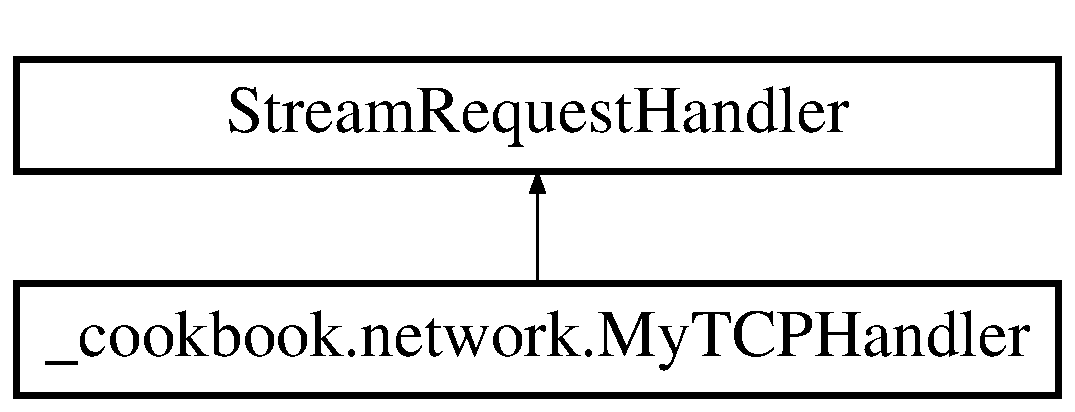
\includegraphics[height=2.000000cm]{dd/d15/class__cookbook_1_1network_1_1MyTCPHandler}
\end{center}
\end{figure}
\subsection*{Public Member Functions}
\begin{DoxyCompactItemize}
\item 
def \hyperlink{class__cookbook_1_1network_1_1MyTCPHandler_a31d7dcf17493e26af74799fc3fbda72a}{handle}
\end{DoxyCompactItemize}
\subsection*{Public Attributes}
\begin{DoxyCompactItemize}
\item 
\hyperlink{class__cookbook_1_1network_1_1MyTCPHandler_ae44f9a12a83a8bb057b192d612bda012}{data}
\end{DoxyCompactItemize}


\subsection{Detailed Description}
\begin{DoxyVerb}TCP handler by framework "SocketServer"
\end{DoxyVerb}
 

Definition at line 388 of file network.\-py.



\subsection{Member Function Documentation}
\hypertarget{class__cookbook_1_1network_1_1MyTCPHandler_a31d7dcf17493e26af74799fc3fbda72a}{\index{\-\_\-cookbook\-::network\-::\-My\-T\-C\-P\-Handler@{\-\_\-cookbook\-::network\-::\-My\-T\-C\-P\-Handler}!handle@{handle}}
\index{handle@{handle}!_cookbook::network::MyTCPHandler@{\-\_\-cookbook\-::network\-::\-My\-T\-C\-P\-Handler}}
\subsubsection[{handle}]{\setlength{\rightskip}{0pt plus 5cm}def \-\_\-cookbook.\-network.\-My\-T\-C\-P\-Handler.\-handle (
\begin{DoxyParamCaption}
\item[{}]{self}
\end{DoxyParamCaption}
)}}\label{class__cookbook_1_1network_1_1MyTCPHandler_a31d7dcf17493e26af74799fc3fbda72a}


Definition at line 391 of file network.\-py.



\subsection{Member Data Documentation}
\hypertarget{class__cookbook_1_1network_1_1MyTCPHandler_ae44f9a12a83a8bb057b192d612bda012}{\index{\-\_\-cookbook\-::network\-::\-My\-T\-C\-P\-Handler@{\-\_\-cookbook\-::network\-::\-My\-T\-C\-P\-Handler}!data@{data}}
\index{data@{data}!_cookbook::network::MyTCPHandler@{\-\_\-cookbook\-::network\-::\-My\-T\-C\-P\-Handler}}
\subsubsection[{data}]{\setlength{\rightskip}{0pt plus 5cm}\-\_\-cookbook.\-network.\-My\-T\-C\-P\-Handler.\-data}}\label{class__cookbook_1_1network_1_1MyTCPHandler_ae44f9a12a83a8bb057b192d612bda012}


Definition at line 395 of file network.\-py.



The documentation for this class was generated from the following file\-:\begin{DoxyCompactItemize}
\item 
\-\_\-cookbook/\hyperlink{network_8py}{network.\-py}\end{DoxyCompactItemize}

\hypertarget{class__cookbook_1_1network_1_1MyTCPServer}{\section{\-\_\-cookbook.\-network.\-My\-T\-C\-P\-Server Class Reference}
\label{class__cookbook_1_1network_1_1MyTCPServer}\index{\-\_\-cookbook.\-network.\-My\-T\-C\-P\-Server@{\-\_\-cookbook.\-network.\-My\-T\-C\-P\-Server}}
}
Inheritance diagram for \-\_\-cookbook.\-network.\-My\-T\-C\-P\-Server\-:\begin{figure}[H]
\begin{center}
\leavevmode
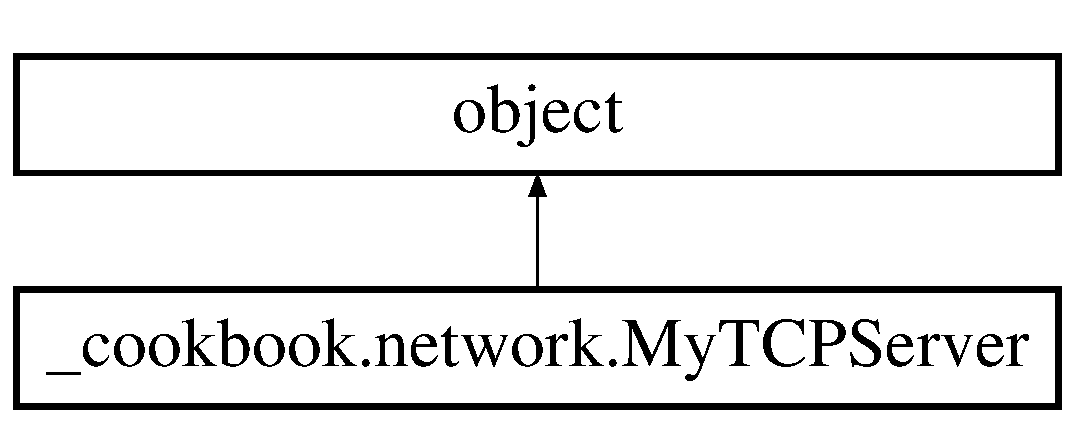
\includegraphics[height=2.000000cm]{d1/dca/class__cookbook_1_1network_1_1MyTCPServer}
\end{center}
\end{figure}
\subsection*{Public Member Functions}
\begin{DoxyCompactItemize}
\item 
def \hyperlink{class__cookbook_1_1network_1_1MyTCPServer_ae4662fa1fa988f518ea3fecfeed42aeb}{\-\_\-\-\_\-init\-\_\-\-\_\-}
\item 
def \hyperlink{class__cookbook_1_1network_1_1MyTCPServer_a4881fd46726e14e995d3f69cc51edbad}{serve\-\_\-forever}
\end{DoxyCompactItemize}
\subsection*{Public Attributes}
\begin{DoxyCompactItemize}
\item 
\hyperlink{class__cookbook_1_1network_1_1MyTCPServer_a5d05dd8cc8114a343c9622b65340ee59}{server\-\_\-address}
\item 
\hyperlink{class__cookbook_1_1network_1_1MyTCPServer_a6ff2e7ff8e8cabc2ea5e57b0c03474b3}{socket}
\end{DoxyCompactItemize}
\subsection*{Static Public Attributes}
\begin{DoxyCompactItemize}
\item 
\hyperlink{class__cookbook_1_1network_1_1MyTCPServer_ae36e3c148d927eaa2a669fa4c2227e0a}{address\-\_\-family} = socket.\-A\-F\-\_\-\-I\-N\-E\-T
\item 
\hyperlink{class__cookbook_1_1network_1_1MyTCPServer_ae7f81da7d2ed969bf5df075b09850879}{socket\-\_\-type} = socket.\-S\-O\-C\-K\-\_\-\-S\-T\-R\-E\-A\-M
\item 
int \hyperlink{class__cookbook_1_1network_1_1MyTCPServer_af80f389b881aac1996ab9258d8507db0}{request\-\_\-queue\-\_\-size} = 5
\end{DoxyCompactItemize}
\subsection*{Private Member Functions}
\begin{DoxyCompactItemize}
\item 
def \hyperlink{class__cookbook_1_1network_1_1MyTCPServer_ac8ca922bd2e669878ef773369fd59f1b}{\-\_\-handle\-\_\-request}
\item 
def \hyperlink{class__cookbook_1_1network_1_1MyTCPServer_a34045163ccbcbe1df6787ccccdf5ccd4}{\-\_\-handle\-\_\-request\-\_\-thread}
\end{DoxyCompactItemize}
\subsection*{Private Attributes}
\begin{DoxyCompactItemize}
\item 
\hyperlink{class__cookbook_1_1network_1_1MyTCPServer_a2d426a06d0a3da094c8034f7fc01d418}{\-\_\-timeout}
\item 
\hyperlink{class__cookbook_1_1network_1_1MyTCPServer_a5de848477fbd96d57b18d29761a86b9e}{\-\_\-buf\-\_\-size}
\end{DoxyCompactItemize}


\subsection{Detailed Description}
\begin{DoxyVerb}TCP Server (Only IPv4).
\end{DoxyVerb}
 

Definition at line 92 of file network.\-py.



\subsection{Constructor \& Destructor Documentation}
\hypertarget{class__cookbook_1_1network_1_1MyTCPServer_ae4662fa1fa988f518ea3fecfeed42aeb}{\index{\-\_\-cookbook\-::network\-::\-My\-T\-C\-P\-Server@{\-\_\-cookbook\-::network\-::\-My\-T\-C\-P\-Server}!\-\_\-\-\_\-init\-\_\-\-\_\-@{\-\_\-\-\_\-init\-\_\-\-\_\-}}
\index{\-\_\-\-\_\-init\-\_\-\-\_\-@{\-\_\-\-\_\-init\-\_\-\-\_\-}!_cookbook::network::MyTCPServer@{\-\_\-cookbook\-::network\-::\-My\-T\-C\-P\-Server}}
\subsubsection[{\-\_\-\-\_\-init\-\_\-\-\_\-}]{\setlength{\rightskip}{0pt plus 5cm}def \-\_\-cookbook.\-network.\-My\-T\-C\-P\-Server.\-\_\-\-\_\-init\-\_\-\-\_\- (
\begin{DoxyParamCaption}
\item[{}]{self, }
\item[{}]{address, }
\item[{}]{buf\-\_\-size = {\ttfamily 1024}, }
\item[{}]{timeout = {\ttfamily None}}
\end{DoxyParamCaption}
)}}\label{class__cookbook_1_1network_1_1MyTCPServer_ae4662fa1fa988f518ea3fecfeed42aeb}
\begin{DoxyVerb}Create an instance of TCP server.

@param address server address, 2-tuple (host, port)
@param buf_size receiving buffer size
@param timeout timeout of socket object. None for blocking, 0.0 for
non-blocking, others for timeout in seconds (float)
@exception socket.error
\end{DoxyVerb}
 

Definition at line 99 of file network.\-py.



\subsection{Member Function Documentation}
\hypertarget{class__cookbook_1_1network_1_1MyTCPServer_ac8ca922bd2e669878ef773369fd59f1b}{\index{\-\_\-cookbook\-::network\-::\-My\-T\-C\-P\-Server@{\-\_\-cookbook\-::network\-::\-My\-T\-C\-P\-Server}!\-\_\-handle\-\_\-request@{\-\_\-handle\-\_\-request}}
\index{\-\_\-handle\-\_\-request@{\-\_\-handle\-\_\-request}!_cookbook::network::MyTCPServer@{\-\_\-cookbook\-::network\-::\-My\-T\-C\-P\-Server}}
\subsubsection[{\-\_\-handle\-\_\-request}]{\setlength{\rightskip}{0pt plus 5cm}def \-\_\-cookbook.\-network.\-My\-T\-C\-P\-Server.\-\_\-handle\-\_\-request (
\begin{DoxyParamCaption}
\item[{}]{self}
\end{DoxyParamCaption}
)\hspace{0.3cm}{\ttfamily [private]}}}\label{class__cookbook_1_1network_1_1MyTCPServer_ac8ca922bd2e669878ef773369fd59f1b}
\begin{DoxyVerb}Handle one request.
\end{DoxyVerb}
 

Definition at line 232 of file network.\-py.

\hypertarget{class__cookbook_1_1network_1_1MyTCPServer_a34045163ccbcbe1df6787ccccdf5ccd4}{\index{\-\_\-cookbook\-::network\-::\-My\-T\-C\-P\-Server@{\-\_\-cookbook\-::network\-::\-My\-T\-C\-P\-Server}!\-\_\-handle\-\_\-request\-\_\-thread@{\-\_\-handle\-\_\-request\-\_\-thread}}
\index{\-\_\-handle\-\_\-request\-\_\-thread@{\-\_\-handle\-\_\-request\-\_\-thread}!_cookbook::network::MyTCPServer@{\-\_\-cookbook\-::network\-::\-My\-T\-C\-P\-Server}}
\subsubsection[{\-\_\-handle\-\_\-request\-\_\-thread}]{\setlength{\rightskip}{0pt plus 5cm}def \-\_\-cookbook.\-network.\-My\-T\-C\-P\-Server.\-\_\-handle\-\_\-request\-\_\-thread (
\begin{DoxyParamCaption}
\item[{}]{self, }
\item[{}]{request}
\end{DoxyParamCaption}
)\hspace{0.3cm}{\ttfamily [private]}}}\label{class__cookbook_1_1network_1_1MyTCPServer_a34045163ccbcbe1df6787ccccdf5ccd4}
\begin{DoxyVerb}Handle each request in a thread.

@param request request from client
\end{DoxyVerb}
 

Definition at line 249 of file network.\-py.

\hypertarget{class__cookbook_1_1network_1_1MyTCPServer_a4881fd46726e14e995d3f69cc51edbad}{\index{\-\_\-cookbook\-::network\-::\-My\-T\-C\-P\-Server@{\-\_\-cookbook\-::network\-::\-My\-T\-C\-P\-Server}!serve\-\_\-forever@{serve\-\_\-forever}}
\index{serve\-\_\-forever@{serve\-\_\-forever}!_cookbook::network::MyTCPServer@{\-\_\-cookbook\-::network\-::\-My\-T\-C\-P\-Server}}
\subsubsection[{serve\-\_\-forever}]{\setlength{\rightskip}{0pt plus 5cm}def \-\_\-cookbook.\-network.\-My\-T\-C\-P\-Server.\-serve\-\_\-forever (
\begin{DoxyParamCaption}
\item[{}]{self, }
\item[{}]{multiplex = {\ttfamily None}, }
\item[{}]{timeout = {\ttfamily 0.5}}
\end{DoxyParamCaption}
)}}\label{class__cookbook_1_1network_1_1MyTCPServer_a4881fd46726e14e995d3f69cc51edbad}
\begin{DoxyVerb}Run server.

@param multiplex I/O multiplexing method: "None", "epoll", "poll", "select".
@param timeout timeout used by POSIX `select()` or poll()` in seconds
@exception select.error

The `poll()` system call, supported on most Unix systems, provides
better scalability for network servers that service many, many clients
at the same time. `poll()` scales better because the system call only
requires listing the file descriptors of interest, while `select()`
builds a bitmap, turns on bits for the fds of interest, and then
afterwards the whole bitmap has to be linearly scanned again. `select()`
is O(highest file descriptor), while poll() is O(number of file
descriptors).

@warnning `epoll()` ONLY available on Linux 2.5+.
\end{DoxyVerb}
 

Definition at line 127 of file network.\-py.



\subsection{Member Data Documentation}
\hypertarget{class__cookbook_1_1network_1_1MyTCPServer_a5de848477fbd96d57b18d29761a86b9e}{\index{\-\_\-cookbook\-::network\-::\-My\-T\-C\-P\-Server@{\-\_\-cookbook\-::network\-::\-My\-T\-C\-P\-Server}!\-\_\-buf\-\_\-size@{\-\_\-buf\-\_\-size}}
\index{\-\_\-buf\-\_\-size@{\-\_\-buf\-\_\-size}!_cookbook::network::MyTCPServer@{\-\_\-cookbook\-::network\-::\-My\-T\-C\-P\-Server}}
\subsubsection[{\-\_\-buf\-\_\-size}]{\setlength{\rightskip}{0pt plus 5cm}\-\_\-cookbook.\-network.\-My\-T\-C\-P\-Server.\-\_\-buf\-\_\-size\hspace{0.3cm}{\ttfamily [private]}}}\label{class__cookbook_1_1network_1_1MyTCPServer_a5de848477fbd96d57b18d29761a86b9e}


Definition at line 110 of file network.\-py.

\hypertarget{class__cookbook_1_1network_1_1MyTCPServer_a2d426a06d0a3da094c8034f7fc01d418}{\index{\-\_\-cookbook\-::network\-::\-My\-T\-C\-P\-Server@{\-\_\-cookbook\-::network\-::\-My\-T\-C\-P\-Server}!\-\_\-timeout@{\-\_\-timeout}}
\index{\-\_\-timeout@{\-\_\-timeout}!_cookbook::network::MyTCPServer@{\-\_\-cookbook\-::network\-::\-My\-T\-C\-P\-Server}}
\subsubsection[{\-\_\-timeout}]{\setlength{\rightskip}{0pt plus 5cm}\-\_\-cookbook.\-network.\-My\-T\-C\-P\-Server.\-\_\-timeout\hspace{0.3cm}{\ttfamily [private]}}}\label{class__cookbook_1_1network_1_1MyTCPServer_a2d426a06d0a3da094c8034f7fc01d418}


Definition at line 109 of file network.\-py.

\hypertarget{class__cookbook_1_1network_1_1MyTCPServer_ae36e3c148d927eaa2a669fa4c2227e0a}{\index{\-\_\-cookbook\-::network\-::\-My\-T\-C\-P\-Server@{\-\_\-cookbook\-::network\-::\-My\-T\-C\-P\-Server}!address\-\_\-family@{address\-\_\-family}}
\index{address\-\_\-family@{address\-\_\-family}!_cookbook::network::MyTCPServer@{\-\_\-cookbook\-::network\-::\-My\-T\-C\-P\-Server}}
\subsubsection[{address\-\_\-family}]{\setlength{\rightskip}{0pt plus 5cm}\-\_\-cookbook.\-network.\-My\-T\-C\-P\-Server.\-address\-\_\-family = socket.\-A\-F\-\_\-\-I\-N\-E\-T\hspace{0.3cm}{\ttfamily [static]}}}\label{class__cookbook_1_1network_1_1MyTCPServer_ae36e3c148d927eaa2a669fa4c2227e0a}


Definition at line 95 of file network.\-py.

\hypertarget{class__cookbook_1_1network_1_1MyTCPServer_af80f389b881aac1996ab9258d8507db0}{\index{\-\_\-cookbook\-::network\-::\-My\-T\-C\-P\-Server@{\-\_\-cookbook\-::network\-::\-My\-T\-C\-P\-Server}!request\-\_\-queue\-\_\-size@{request\-\_\-queue\-\_\-size}}
\index{request\-\_\-queue\-\_\-size@{request\-\_\-queue\-\_\-size}!_cookbook::network::MyTCPServer@{\-\_\-cookbook\-::network\-::\-My\-T\-C\-P\-Server}}
\subsubsection[{request\-\_\-queue\-\_\-size}]{\setlength{\rightskip}{0pt plus 5cm}int \-\_\-cookbook.\-network.\-My\-T\-C\-P\-Server.\-request\-\_\-queue\-\_\-size = 5\hspace{0.3cm}{\ttfamily [static]}}}\label{class__cookbook_1_1network_1_1MyTCPServer_af80f389b881aac1996ab9258d8507db0}


Definition at line 97 of file network.\-py.

\hypertarget{class__cookbook_1_1network_1_1MyTCPServer_a5d05dd8cc8114a343c9622b65340ee59}{\index{\-\_\-cookbook\-::network\-::\-My\-T\-C\-P\-Server@{\-\_\-cookbook\-::network\-::\-My\-T\-C\-P\-Server}!server\-\_\-address@{server\-\_\-address}}
\index{server\-\_\-address@{server\-\_\-address}!_cookbook::network::MyTCPServer@{\-\_\-cookbook\-::network\-::\-My\-T\-C\-P\-Server}}
\subsubsection[{server\-\_\-address}]{\setlength{\rightskip}{0pt plus 5cm}\-\_\-cookbook.\-network.\-My\-T\-C\-P\-Server.\-server\-\_\-address}}\label{class__cookbook_1_1network_1_1MyTCPServer_a5d05dd8cc8114a343c9622b65340ee59}


Definition at line 108 of file network.\-py.

\hypertarget{class__cookbook_1_1network_1_1MyTCPServer_a6ff2e7ff8e8cabc2ea5e57b0c03474b3}{\index{\-\_\-cookbook\-::network\-::\-My\-T\-C\-P\-Server@{\-\_\-cookbook\-::network\-::\-My\-T\-C\-P\-Server}!socket@{socket}}
\index{socket@{socket}!_cookbook::network::MyTCPServer@{\-\_\-cookbook\-::network\-::\-My\-T\-C\-P\-Server}}
\subsubsection[{socket}]{\setlength{\rightskip}{0pt plus 5cm}\-\_\-cookbook.\-network.\-My\-T\-C\-P\-Server.\-socket}}\label{class__cookbook_1_1network_1_1MyTCPServer_a6ff2e7ff8e8cabc2ea5e57b0c03474b3}


Definition at line 113 of file network.\-py.

\hypertarget{class__cookbook_1_1network_1_1MyTCPServer_ae7f81da7d2ed969bf5df075b09850879}{\index{\-\_\-cookbook\-::network\-::\-My\-T\-C\-P\-Server@{\-\_\-cookbook\-::network\-::\-My\-T\-C\-P\-Server}!socket\-\_\-type@{socket\-\_\-type}}
\index{socket\-\_\-type@{socket\-\_\-type}!_cookbook::network::MyTCPServer@{\-\_\-cookbook\-::network\-::\-My\-T\-C\-P\-Server}}
\subsubsection[{socket\-\_\-type}]{\setlength{\rightskip}{0pt plus 5cm}\-\_\-cookbook.\-network.\-My\-T\-C\-P\-Server.\-socket\-\_\-type = socket.\-S\-O\-C\-K\-\_\-\-S\-T\-R\-E\-A\-M\hspace{0.3cm}{\ttfamily [static]}}}\label{class__cookbook_1_1network_1_1MyTCPServer_ae7f81da7d2ed969bf5df075b09850879}


Definition at line 96 of file network.\-py.



The documentation for this class was generated from the following file\-:\begin{DoxyCompactItemize}
\item 
\-\_\-cookbook/\hyperlink{network_8py}{network.\-py}\end{DoxyCompactItemize}

\hypertarget{class__cookbook_1_1thread_1_1lock_1_1MyThread}{\section{\-\_\-cookbook.\-thread.\-lock.\-My\-Thread Class Reference}
\label{class__cookbook_1_1thread_1_1lock_1_1MyThread}\index{\-\_\-cookbook.\-thread.\-lock.\-My\-Thread@{\-\_\-cookbook.\-thread.\-lock.\-My\-Thread}}
}
Inheritance diagram for \-\_\-cookbook.\-thread.\-lock.\-My\-Thread\-:\begin{figure}[H]
\begin{center}
\leavevmode
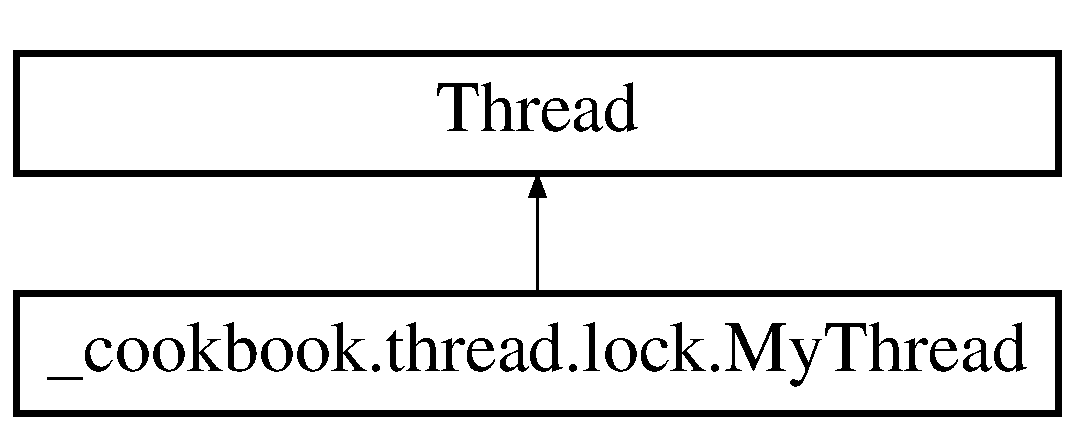
\includegraphics[height=2.000000cm]{df/d25/class__cookbook_1_1thread_1_1lock_1_1MyThread}
\end{center}
\end{figure}
\subsection*{Public Member Functions}
\begin{DoxyCompactItemize}
\item 
def \hyperlink{class__cookbook_1_1thread_1_1lock_1_1MyThread_af2698f3a89f72d901670df8bd7050b88}{\-\_\-\-\_\-init\-\_\-\-\_\-}
\item 
def \hyperlink{class__cookbook_1_1thread_1_1lock_1_1MyThread_add32daaabfa40fefc9f0a21bdd7af098}{run}
\end{DoxyCompactItemize}
\subsection*{Public Attributes}
\begin{DoxyCompactItemize}
\item 
\hyperlink{class__cookbook_1_1thread_1_1lock_1_1MyThread_a91f0432528c15cb2a108aa527672709a}{arg}
\end{DoxyCompactItemize}


\subsection{Detailed Description}


Definition at line 46 of file lock.\-py.



\subsection{Constructor \& Destructor Documentation}
\hypertarget{class__cookbook_1_1thread_1_1lock_1_1MyThread_af2698f3a89f72d901670df8bd7050b88}{\index{\-\_\-cookbook\-::thread\-::lock\-::\-My\-Thread@{\-\_\-cookbook\-::thread\-::lock\-::\-My\-Thread}!\-\_\-\-\_\-init\-\_\-\-\_\-@{\-\_\-\-\_\-init\-\_\-\-\_\-}}
\index{\-\_\-\-\_\-init\-\_\-\-\_\-@{\-\_\-\-\_\-init\-\_\-\-\_\-}!_cookbook::thread::lock::MyThread@{\-\_\-cookbook\-::thread\-::lock\-::\-My\-Thread}}
\subsubsection[{\-\_\-\-\_\-init\-\_\-\-\_\-}]{\setlength{\rightskip}{0pt plus 5cm}def \-\_\-cookbook.\-thread.\-lock.\-My\-Thread.\-\_\-\-\_\-init\-\_\-\-\_\- (
\begin{DoxyParamCaption}
\item[{}]{self, }
\item[{}]{arg, }
\item[{}]{name = {\ttfamily None}}
\end{DoxyParamCaption}
)}}\label{class__cookbook_1_1thread_1_1lock_1_1MyThread_af2698f3a89f72d901670df8bd7050b88}


Definition at line 47 of file lock.\-py.



\subsection{Member Function Documentation}
\hypertarget{class__cookbook_1_1thread_1_1lock_1_1MyThread_add32daaabfa40fefc9f0a21bdd7af098}{\index{\-\_\-cookbook\-::thread\-::lock\-::\-My\-Thread@{\-\_\-cookbook\-::thread\-::lock\-::\-My\-Thread}!run@{run}}
\index{run@{run}!_cookbook::thread::lock::MyThread@{\-\_\-cookbook\-::thread\-::lock\-::\-My\-Thread}}
\subsubsection[{run}]{\setlength{\rightskip}{0pt plus 5cm}def \-\_\-cookbook.\-thread.\-lock.\-My\-Thread.\-run (
\begin{DoxyParamCaption}
\item[{}]{self}
\end{DoxyParamCaption}
)}}\label{class__cookbook_1_1thread_1_1lock_1_1MyThread_add32daaabfa40fefc9f0a21bdd7af098}


Definition at line 52 of file lock.\-py.



\subsection{Member Data Documentation}
\hypertarget{class__cookbook_1_1thread_1_1lock_1_1MyThread_a91f0432528c15cb2a108aa527672709a}{\index{\-\_\-cookbook\-::thread\-::lock\-::\-My\-Thread@{\-\_\-cookbook\-::thread\-::lock\-::\-My\-Thread}!arg@{arg}}
\index{arg@{arg}!_cookbook::thread::lock::MyThread@{\-\_\-cookbook\-::thread\-::lock\-::\-My\-Thread}}
\subsubsection[{arg}]{\setlength{\rightskip}{0pt plus 5cm}\-\_\-cookbook.\-thread.\-lock.\-My\-Thread.\-arg}}\label{class__cookbook_1_1thread_1_1lock_1_1MyThread_a91f0432528c15cb2a108aa527672709a}


Definition at line 49 of file lock.\-py.



The documentation for this class was generated from the following file\-:\begin{DoxyCompactItemize}
\item 
\-\_\-cookbook/thread/\hyperlink{lock_8py}{lock.\-py}\end{DoxyCompactItemize}

\hypertarget{class__cookbook_1_1network_1_1MyUDPServer}{\section{\-\_\-cookbook.\-network.\-My\-U\-D\-P\-Server Class Reference}
\label{class__cookbook_1_1network_1_1MyUDPServer}\index{\-\_\-cookbook.\-network.\-My\-U\-D\-P\-Server@{\-\_\-cookbook.\-network.\-My\-U\-D\-P\-Server}}
}
Inheritance diagram for \-\_\-cookbook.\-network.\-My\-U\-D\-P\-Server\-:\begin{figure}[H]
\begin{center}
\leavevmode
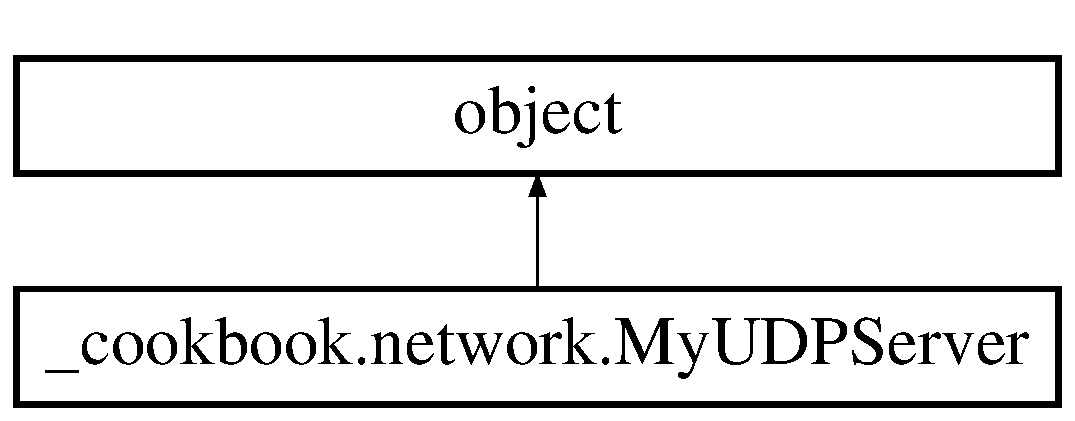
\includegraphics[height=2.000000cm]{d0/d63/class__cookbook_1_1network_1_1MyUDPServer}
\end{center}
\end{figure}
\subsection*{Public Member Functions}
\begin{DoxyCompactItemize}
\item 
def \hyperlink{class__cookbook_1_1network_1_1MyUDPServer_a5fd05dec49b0b2be004d5de49b22fc27}{\-\_\-\-\_\-init\-\_\-\-\_\-}
\item 
def \hyperlink{class__cookbook_1_1network_1_1MyUDPServer_a1463759224a77649cd1ba2f4bf6fba8d}{serve\-\_\-forever}
\end{DoxyCompactItemize}
\subsection*{Public Attributes}
\begin{DoxyCompactItemize}
\item 
\hyperlink{class__cookbook_1_1network_1_1MyUDPServer_aed17e4556fb33e07bc8a348aedf63ae4}{server\-\_\-address}
\item 
\hyperlink{class__cookbook_1_1network_1_1MyUDPServer_aeae33e7df31d329cd74f78f195b5753b}{socket}
\end{DoxyCompactItemize}
\subsection*{Static Public Attributes}
\begin{DoxyCompactItemize}
\item 
\hyperlink{class__cookbook_1_1network_1_1MyUDPServer_a4b7d2c6b542b30c47bf020647b8685f9}{address\-\_\-family} = socket.\-A\-F\-\_\-\-I\-N\-E\-T
\item 
\hyperlink{class__cookbook_1_1network_1_1MyUDPServer_ad01d41f36b9e554d7ca247c3ab677511}{socket\-\_\-type} = socket.\-S\-O\-C\-K\-\_\-\-D\-G\-R\-A\-M
\end{DoxyCompactItemize}
\subsection*{Private Attributes}
\begin{DoxyCompactItemize}
\item 
\hyperlink{class__cookbook_1_1network_1_1MyUDPServer_ab9d1f00ec5ba408d0cf00230e820d04d}{\-\_\-buf\-\_\-size}
\end{DoxyCompactItemize}


\subsection{Detailed Description}
\begin{DoxyVerb}Synchronous UDP Server (Only IPv4).
\end{DoxyVerb}
 

Definition at line 272 of file network.\-py.



\subsection{Constructor \& Destructor Documentation}
\hypertarget{class__cookbook_1_1network_1_1MyUDPServer_a5fd05dec49b0b2be004d5de49b22fc27}{\index{\-\_\-cookbook\-::network\-::\-My\-U\-D\-P\-Server@{\-\_\-cookbook\-::network\-::\-My\-U\-D\-P\-Server}!\-\_\-\-\_\-init\-\_\-\-\_\-@{\-\_\-\-\_\-init\-\_\-\-\_\-}}
\index{\-\_\-\-\_\-init\-\_\-\-\_\-@{\-\_\-\-\_\-init\-\_\-\-\_\-}!_cookbook::network::MyUDPServer@{\-\_\-cookbook\-::network\-::\-My\-U\-D\-P\-Server}}
\subsubsection[{\-\_\-\-\_\-init\-\_\-\-\_\-}]{\setlength{\rightskip}{0pt plus 5cm}def \-\_\-cookbook.\-network.\-My\-U\-D\-P\-Server.\-\_\-\-\_\-init\-\_\-\-\_\- (
\begin{DoxyParamCaption}
\item[{}]{self, }
\item[{}]{address, }
\item[{}]{buf\-\_\-size = {\ttfamily 1024}}
\end{DoxyParamCaption}
)}}\label{class__cookbook_1_1network_1_1MyUDPServer_a5fd05dec49b0b2be004d5de49b22fc27}
\begin{DoxyVerb}Create an instance of UDP server.

@param address server address, 2-tuple (host, port)
@param buf_size receiving buffer size
@exception socket.error
\end{DoxyVerb}
 

Definition at line 278 of file network.\-py.



\subsection{Member Function Documentation}
\hypertarget{class__cookbook_1_1network_1_1MyUDPServer_a1463759224a77649cd1ba2f4bf6fba8d}{\index{\-\_\-cookbook\-::network\-::\-My\-U\-D\-P\-Server@{\-\_\-cookbook\-::network\-::\-My\-U\-D\-P\-Server}!serve\-\_\-forever@{serve\-\_\-forever}}
\index{serve\-\_\-forever@{serve\-\_\-forever}!_cookbook::network::MyUDPServer@{\-\_\-cookbook\-::network\-::\-My\-U\-D\-P\-Server}}
\subsubsection[{serve\-\_\-forever}]{\setlength{\rightskip}{0pt plus 5cm}def \-\_\-cookbook.\-network.\-My\-U\-D\-P\-Server.\-serve\-\_\-forever (
\begin{DoxyParamCaption}
\item[{}]{self}
\end{DoxyParamCaption}
)}}\label{class__cookbook_1_1network_1_1MyUDPServer_a1463759224a77649cd1ba2f4bf6fba8d}
\begin{DoxyVerb}Run server.
\end{DoxyVerb}
 

Definition at line 295 of file network.\-py.



\subsection{Member Data Documentation}
\hypertarget{class__cookbook_1_1network_1_1MyUDPServer_ab9d1f00ec5ba408d0cf00230e820d04d}{\index{\-\_\-cookbook\-::network\-::\-My\-U\-D\-P\-Server@{\-\_\-cookbook\-::network\-::\-My\-U\-D\-P\-Server}!\-\_\-buf\-\_\-size@{\-\_\-buf\-\_\-size}}
\index{\-\_\-buf\-\_\-size@{\-\_\-buf\-\_\-size}!_cookbook::network::MyUDPServer@{\-\_\-cookbook\-::network\-::\-My\-U\-D\-P\-Server}}
\subsubsection[{\-\_\-buf\-\_\-size}]{\setlength{\rightskip}{0pt plus 5cm}\-\_\-cookbook.\-network.\-My\-U\-D\-P\-Server.\-\_\-buf\-\_\-size\hspace{0.3cm}{\ttfamily [private]}}}\label{class__cookbook_1_1network_1_1MyUDPServer_ab9d1f00ec5ba408d0cf00230e820d04d}


Definition at line 286 of file network.\-py.

\hypertarget{class__cookbook_1_1network_1_1MyUDPServer_a4b7d2c6b542b30c47bf020647b8685f9}{\index{\-\_\-cookbook\-::network\-::\-My\-U\-D\-P\-Server@{\-\_\-cookbook\-::network\-::\-My\-U\-D\-P\-Server}!address\-\_\-family@{address\-\_\-family}}
\index{address\-\_\-family@{address\-\_\-family}!_cookbook::network::MyUDPServer@{\-\_\-cookbook\-::network\-::\-My\-U\-D\-P\-Server}}
\subsubsection[{address\-\_\-family}]{\setlength{\rightskip}{0pt plus 5cm}\-\_\-cookbook.\-network.\-My\-U\-D\-P\-Server.\-address\-\_\-family = socket.\-A\-F\-\_\-\-I\-N\-E\-T\hspace{0.3cm}{\ttfamily [static]}}}\label{class__cookbook_1_1network_1_1MyUDPServer_a4b7d2c6b542b30c47bf020647b8685f9}


Definition at line 275 of file network.\-py.

\hypertarget{class__cookbook_1_1network_1_1MyUDPServer_aed17e4556fb33e07bc8a348aedf63ae4}{\index{\-\_\-cookbook\-::network\-::\-My\-U\-D\-P\-Server@{\-\_\-cookbook\-::network\-::\-My\-U\-D\-P\-Server}!server\-\_\-address@{server\-\_\-address}}
\index{server\-\_\-address@{server\-\_\-address}!_cookbook::network::MyUDPServer@{\-\_\-cookbook\-::network\-::\-My\-U\-D\-P\-Server}}
\subsubsection[{server\-\_\-address}]{\setlength{\rightskip}{0pt plus 5cm}\-\_\-cookbook.\-network.\-My\-U\-D\-P\-Server.\-server\-\_\-address}}\label{class__cookbook_1_1network_1_1MyUDPServer_aed17e4556fb33e07bc8a348aedf63ae4}


Definition at line 285 of file network.\-py.

\hypertarget{class__cookbook_1_1network_1_1MyUDPServer_aeae33e7df31d329cd74f78f195b5753b}{\index{\-\_\-cookbook\-::network\-::\-My\-U\-D\-P\-Server@{\-\_\-cookbook\-::network\-::\-My\-U\-D\-P\-Server}!socket@{socket}}
\index{socket@{socket}!_cookbook::network::MyUDPServer@{\-\_\-cookbook\-::network\-::\-My\-U\-D\-P\-Server}}
\subsubsection[{socket}]{\setlength{\rightskip}{0pt plus 5cm}\-\_\-cookbook.\-network.\-My\-U\-D\-P\-Server.\-socket}}\label{class__cookbook_1_1network_1_1MyUDPServer_aeae33e7df31d329cd74f78f195b5753b}


Definition at line 289 of file network.\-py.

\hypertarget{class__cookbook_1_1network_1_1MyUDPServer_ad01d41f36b9e554d7ca247c3ab677511}{\index{\-\_\-cookbook\-::network\-::\-My\-U\-D\-P\-Server@{\-\_\-cookbook\-::network\-::\-My\-U\-D\-P\-Server}!socket\-\_\-type@{socket\-\_\-type}}
\index{socket\-\_\-type@{socket\-\_\-type}!_cookbook::network::MyUDPServer@{\-\_\-cookbook\-::network\-::\-My\-U\-D\-P\-Server}}
\subsubsection[{socket\-\_\-type}]{\setlength{\rightskip}{0pt plus 5cm}\-\_\-cookbook.\-network.\-My\-U\-D\-P\-Server.\-socket\-\_\-type = socket.\-S\-O\-C\-K\-\_\-\-D\-G\-R\-A\-M\hspace{0.3cm}{\ttfamily [static]}}}\label{class__cookbook_1_1network_1_1MyUDPServer_ad01d41f36b9e554d7ca247c3ab677511}


Definition at line 276 of file network.\-py.



The documentation for this class was generated from the following file\-:\begin{DoxyCompactItemize}
\item 
\-\_\-cookbook/\hyperlink{network_8py}{network.\-py}\end{DoxyCompactItemize}

\hypertarget{classadmin_1_1www_1_1nginx}{\section{admin.\-www.\-nginx Class Reference}
\label{classadmin_1_1www_1_1nginx}\index{admin.\-www.\-nginx@{admin.\-www.\-nginx}}
}


nginx server.  


Inheritance diagram for admin.\-www.\-nginx\-:\begin{figure}[H]
\begin{center}
\leavevmode
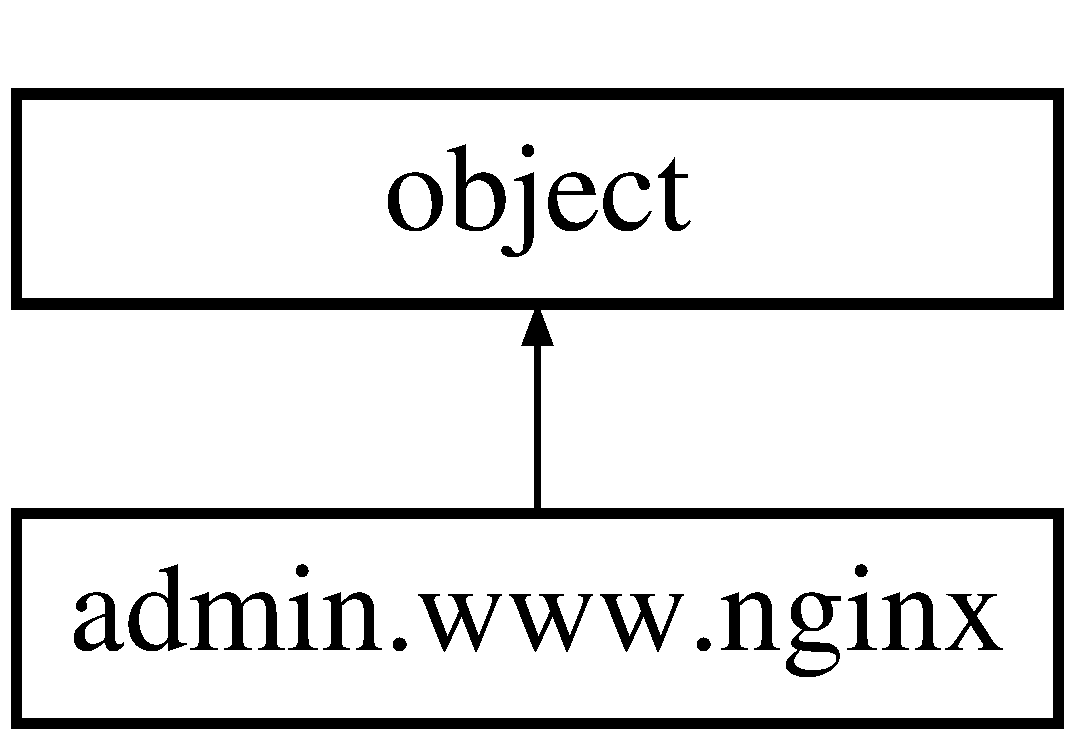
\includegraphics[height=2.000000cm]{dc/db8/classadmin_1_1www_1_1nginx}
\end{center}
\end{figure}
\subsection*{Public Member Functions}
\begin{DoxyCompactItemize}
\item 
def \hyperlink{classadmin_1_1www_1_1nginx_a6d55a9d2645ebdd32a86f07caa30e54f}{enable}
\begin{DoxyCompactList}\small\item\em Setup nginx. \end{DoxyCompactList}\item 
def \hyperlink{classadmin_1_1www_1_1nginx_a97b2603a64e0758b3d548bc1971dcc4e}{disable}
\begin{DoxyCompactList}\small\item\em Disable nginx server. \end{DoxyCompactList}\end{DoxyCompactItemize}
\subsection*{Static Public Attributes}
\begin{DoxyCompactItemize}
\item 
string \hyperlink{classadmin_1_1www_1_1nginx_a0345aad76d9ddd6469c13bef207a9766}{site\-\_\-avail\-\_\-root} = '/etc/\hyperlink{classadmin_1_1www_1_1nginx}{nginx}/sites-\/available'
\item 
string \hyperlink{classadmin_1_1www_1_1nginx_a3e1b0fbd45f31aaeacb6baaec80806ce}{site\-\_\-enable\-\_\-root} = '/etc/\hyperlink{classadmin_1_1www_1_1nginx}{nginx}/sites-\/enabled'
\item 
string \hyperlink{classadmin_1_1www_1_1nginx_aec1e7959ddfe6598718fb6c8c9d72320}{uwsgi\-\_\-params\-\_\-url} = 'https\-://raw.\-githubusercontent.\-com/\hyperlink{classadmin_1_1www_1_1nginx}{nginx}/\hyperlink{classadmin_1_1www_1_1nginx}{nginx}/master/conf/uwsgi\-\_\-params'
\item 
string \hyperlink{classadmin_1_1www_1_1nginx_afd444548cd6faf42c56e24e22148a4b4}{uwsgi\-\_\-params\-\_\-path} = '/etc/\hyperlink{classadmin_1_1www_1_1nginx}{nginx}/uwsgi\-\_\-params'
\end{DoxyCompactItemize}
\subsection*{Private Member Functions}
\begin{DoxyCompactItemize}
\item 
def \hyperlink{classadmin_1_1www_1_1nginx_aca978777776a324a0c3ac506100da002}{\-\_\-site\-\_\-avail\-\_\-path}
\begin{DoxyCompactList}\small\item\em Return path of available site by name. \end{DoxyCompactList}\item 
def \hyperlink{classadmin_1_1www_1_1nginx_af4bc4f7da3d2c56ba8e4b61b16052394}{\-\_\-site\-\_\-enable\-\_\-path}
\begin{DoxyCompactList}\small\item\em Return path of enabled site by name. \end{DoxyCompactList}\end{DoxyCompactItemize}


\subsection{Detailed Description}
nginx server. 

\begin{DoxySeeAlso}{See Also}
\href{http://wiki.nginx.org/Pitfalls}{\tt http\-://wiki.\-nginx.\-org/\-Pitfalls} 

\href{http://wiki.nginx.org/QuickStart}{\tt http\-://wiki.\-nginx.\-org/\-Quick\-Start} 

\href{http://wiki.nginx.org/Configuration}{\tt http\-://wiki.\-nginx.\-org/\-Configuration} 
\end{DoxySeeAlso}
\begin{DoxySince}{Since}
nginx 1.\-4.\-6 
\end{DoxySince}


Definition at line 567 of file admin.\-py.



\subsection{Member Function Documentation}
\hypertarget{classadmin_1_1www_1_1nginx_aca978777776a324a0c3ac506100da002}{\index{admin\-::www\-::nginx@{admin\-::www\-::nginx}!\-\_\-site\-\_\-avail\-\_\-path@{\-\_\-site\-\_\-avail\-\_\-path}}
\index{\-\_\-site\-\_\-avail\-\_\-path@{\-\_\-site\-\_\-avail\-\_\-path}!admin::www::nginx@{admin\-::www\-::nginx}}
\subsubsection[{\-\_\-site\-\_\-avail\-\_\-path}]{\setlength{\rightskip}{0pt plus 5cm}def admin.\-www.\-nginx.\-\_\-site\-\_\-avail\-\_\-path (
\begin{DoxyParamCaption}
\item[{}]{cls, }
\item[{}]{site\-\_\-name}
\end{DoxyParamCaption}
)\hspace{0.3cm}{\ttfamily [private]}}}\label{classadmin_1_1www_1_1nginx_aca978777776a324a0c3ac506100da002}


Return path of available site by name. 


\begin{DoxyParams}{Parameters}
{\em site\-\_\-name} & site name \\
\hline
\end{DoxyParams}
\begin{DoxyReturn}{Returns}
path of given site 
\end{DoxyReturn}


Definition at line 704 of file admin.\-py.

\hypertarget{classadmin_1_1www_1_1nginx_af4bc4f7da3d2c56ba8e4b61b16052394}{\index{admin\-::www\-::nginx@{admin\-::www\-::nginx}!\-\_\-site\-\_\-enable\-\_\-path@{\-\_\-site\-\_\-enable\-\_\-path}}
\index{\-\_\-site\-\_\-enable\-\_\-path@{\-\_\-site\-\_\-enable\-\_\-path}!admin::www::nginx@{admin\-::www\-::nginx}}
\subsubsection[{\-\_\-site\-\_\-enable\-\_\-path}]{\setlength{\rightskip}{0pt plus 5cm}def admin.\-www.\-nginx.\-\_\-site\-\_\-enable\-\_\-path (
\begin{DoxyParamCaption}
\item[{}]{cls, }
\item[{}]{site\-\_\-name = {\ttfamily None}}
\end{DoxyParamCaption}
)\hspace{0.3cm}{\ttfamily [private]}}}\label{classadmin_1_1www_1_1nginx_af4bc4f7da3d2c56ba8e4b61b16052394}


Return path of enabled site by name. 


\begin{DoxyParams}{Parameters}
{\em site\-\_\-name} & site name \\
\hline
\end{DoxyParams}
\begin{DoxyReturn}{Returns}
path of given site 
\end{DoxyReturn}


Definition at line 713 of file admin.\-py.

\hypertarget{classadmin_1_1www_1_1nginx_a97b2603a64e0758b3d548bc1971dcc4e}{\index{admin\-::www\-::nginx@{admin\-::www\-::nginx}!disable@{disable}}
\index{disable@{disable}!admin::www::nginx@{admin\-::www\-::nginx}}
\subsubsection[{disable}]{\setlength{\rightskip}{0pt plus 5cm}def admin.\-www.\-nginx.\-disable (
\begin{DoxyParamCaption}
\item[{}]{cls, }
\item[{}]{site = {\ttfamily None}, }
\item[{}]{upstream = {\ttfamily None}}
\end{DoxyParamCaption}
)}}\label{classadmin_1_1www_1_1nginx_a97b2603a64e0758b3d548bc1971dcc4e}


Disable nginx server. 


\begin{DoxyParams}{Parameters}
{\em site} & site path \\
\hline
{\em upstream} & upstream host address (u\-W\-S\-G\-I gateway) \\
\hline
\end{DoxyParams}

\begin{DoxyExceptions}{Exceptions}
{\em Admin\-Error(subprocess.\-Called\-Process\-Error)} & -\/ shell {\ttfamily sudo ln -\/sf} or {\ttfamily sudo /etc/init.d} error \\
\hline
\end{DoxyExceptions}


Definition at line 688 of file admin.\-py.

\hypertarget{classadmin_1_1www_1_1nginx_a6d55a9d2645ebdd32a86f07caa30e54f}{\index{admin\-::www\-::nginx@{admin\-::www\-::nginx}!enable@{enable}}
\index{enable@{enable}!admin::www::nginx@{admin\-::www\-::nginx}}
\subsubsection[{enable}]{\setlength{\rightskip}{0pt plus 5cm}def admin.\-www.\-nginx.\-enable (
\begin{DoxyParamCaption}
\item[{}]{cls, }
\item[{}]{site, }
\item[{}]{port = {\ttfamily 80}, }
\item[{}]{name = {\ttfamily 'localhost'}, }
\item[{}]{upstream = {\ttfamily None}, }
\item[{}]{proxy = {\ttfamily '\-:8080'}}
\end{DoxyParamCaption}
)}}\label{classadmin_1_1www_1_1nginx_a6d55a9d2645ebdd32a86f07caa30e54f}


Setup nginx. 


\begin{DoxyParams}{Parameters}
{\em site} & site path \\
\hline
{\em port} & site port number \\
\hline
{\em name} & site server name \\
\hline
{\em upstream} & upstream host address (u\-W\-S\-G\-I gateway) \\
\hline
\end{DoxyParams}

\begin{DoxyExceptions}{Exceptions}
{\em I\-O\-Error} & -\/ site configuration file error \\
\hline
{\em Admin\-Error(subprocess.\-Called\-Process\-Error)} & -\/ shell {\ttfamily sudo mv} error \\
\hline
{\em Admin\-Error(subprocess.\-Called\-Process\-Error)} & -\/ download uwsgi\-\_\-params file error \\
\hline
\end{DoxyExceptions}


Definition at line 584 of file admin.\-py.



\subsection{Member Data Documentation}
\hypertarget{classadmin_1_1www_1_1nginx_a0345aad76d9ddd6469c13bef207a9766}{\index{admin\-::www\-::nginx@{admin\-::www\-::nginx}!site\-\_\-avail\-\_\-root@{site\-\_\-avail\-\_\-root}}
\index{site\-\_\-avail\-\_\-root@{site\-\_\-avail\-\_\-root}!admin::www::nginx@{admin\-::www\-::nginx}}
\subsubsection[{site\-\_\-avail\-\_\-root}]{\setlength{\rightskip}{0pt plus 5cm}string admin.\-www.\-nginx.\-site\-\_\-avail\-\_\-root = '/etc/{\bf nginx}/sites-\/available'\hspace{0.3cm}{\ttfamily [static]}}}\label{classadmin_1_1www_1_1nginx_a0345aad76d9ddd6469c13bef207a9766}


Definition at line 569 of file admin.\-py.

\hypertarget{classadmin_1_1www_1_1nginx_a3e1b0fbd45f31aaeacb6baaec80806ce}{\index{admin\-::www\-::nginx@{admin\-::www\-::nginx}!site\-\_\-enable\-\_\-root@{site\-\_\-enable\-\_\-root}}
\index{site\-\_\-enable\-\_\-root@{site\-\_\-enable\-\_\-root}!admin::www::nginx@{admin\-::www\-::nginx}}
\subsubsection[{site\-\_\-enable\-\_\-root}]{\setlength{\rightskip}{0pt plus 5cm}string admin.\-www.\-nginx.\-site\-\_\-enable\-\_\-root = '/etc/{\bf nginx}/sites-\/enabled'\hspace{0.3cm}{\ttfamily [static]}}}\label{classadmin_1_1www_1_1nginx_a3e1b0fbd45f31aaeacb6baaec80806ce}


Definition at line 570 of file admin.\-py.

\hypertarget{classadmin_1_1www_1_1nginx_afd444548cd6faf42c56e24e22148a4b4}{\index{admin\-::www\-::nginx@{admin\-::www\-::nginx}!uwsgi\-\_\-params\-\_\-path@{uwsgi\-\_\-params\-\_\-path}}
\index{uwsgi\-\_\-params\-\_\-path@{uwsgi\-\_\-params\-\_\-path}!admin::www::nginx@{admin\-::www\-::nginx}}
\subsubsection[{uwsgi\-\_\-params\-\_\-path}]{\setlength{\rightskip}{0pt plus 5cm}string admin.\-www.\-nginx.\-uwsgi\-\_\-params\-\_\-path = '/etc/{\bf nginx}/uwsgi\-\_\-params'\hspace{0.3cm}{\ttfamily [static]}}}\label{classadmin_1_1www_1_1nginx_afd444548cd6faf42c56e24e22148a4b4}


Definition at line 572 of file admin.\-py.

\hypertarget{classadmin_1_1www_1_1nginx_aec1e7959ddfe6598718fb6c8c9d72320}{\index{admin\-::www\-::nginx@{admin\-::www\-::nginx}!uwsgi\-\_\-params\-\_\-url@{uwsgi\-\_\-params\-\_\-url}}
\index{uwsgi\-\_\-params\-\_\-url@{uwsgi\-\_\-params\-\_\-url}!admin::www::nginx@{admin\-::www\-::nginx}}
\subsubsection[{uwsgi\-\_\-params\-\_\-url}]{\setlength{\rightskip}{0pt plus 5cm}string admin.\-www.\-nginx.\-uwsgi\-\_\-params\-\_\-url = 'https\-://raw.\-githubusercontent.\-com/{\bf nginx}/{\bf nginx}/master/conf/uwsgi\-\_\-params'\hspace{0.3cm}{\ttfamily [static]}}}\label{classadmin_1_1www_1_1nginx_aec1e7959ddfe6598718fb6c8c9d72320}


Definition at line 571 of file admin.\-py.



The documentation for this class was generated from the following file\-:\begin{DoxyCompactItemize}
\item 
\hyperlink{admin_8py}{admin.\-py}\end{DoxyCompactItemize}

\hypertarget{class__cookbook_1_1thread_1_1semaphore_1_1Producer}{\section{\-\_\-cookbook.\-thread.\-semaphore.\-Producer Class Reference}
\label{class__cookbook_1_1thread_1_1semaphore_1_1Producer}\index{\-\_\-cookbook.\-thread.\-semaphore.\-Producer@{\-\_\-cookbook.\-thread.\-semaphore.\-Producer}}
}
Inheritance diagram for \-\_\-cookbook.\-thread.\-semaphore.\-Producer\-:\begin{figure}[H]
\begin{center}
\leavevmode
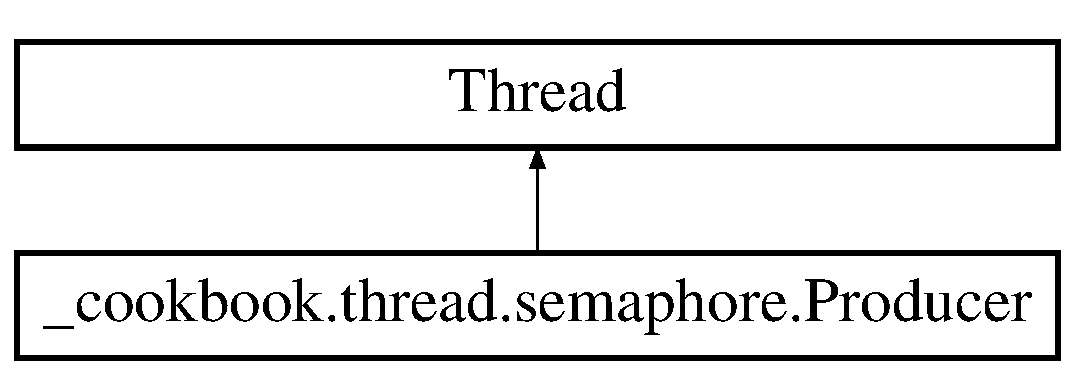
\includegraphics[height=2.000000cm]{dc/ddd/class__cookbook_1_1thread_1_1semaphore_1_1Producer}
\end{center}
\end{figure}
\subsection*{Public Member Functions}
\begin{DoxyCompactItemize}
\item 
def \hyperlink{class__cookbook_1_1thread_1_1semaphore_1_1Producer_a90c647987606af89572fb06cc99264a4}{\-\_\-\-\_\-init\-\_\-\-\_\-}
\item 
def \hyperlink{class__cookbook_1_1thread_1_1semaphore_1_1Producer_a28b97d68456cbad8eb0938dd36cae1db}{run}
\end{DoxyCompactItemize}
\subsection*{Public Attributes}
\begin{DoxyCompactItemize}
\item 
\hyperlink{class__cookbook_1_1thread_1_1semaphore_1_1Producer_ad9bb19976d4019473b25933e8589fb95}{arg}
\end{DoxyCompactItemize}


\subsection{Detailed Description}


Definition at line 42 of file semaphore.\-py.



\subsection{Constructor \& Destructor Documentation}
\hypertarget{class__cookbook_1_1thread_1_1semaphore_1_1Producer_a90c647987606af89572fb06cc99264a4}{\index{\-\_\-cookbook\-::thread\-::semaphore\-::\-Producer@{\-\_\-cookbook\-::thread\-::semaphore\-::\-Producer}!\-\_\-\-\_\-init\-\_\-\-\_\-@{\-\_\-\-\_\-init\-\_\-\-\_\-}}
\index{\-\_\-\-\_\-init\-\_\-\-\_\-@{\-\_\-\-\_\-init\-\_\-\-\_\-}!_cookbook::thread::semaphore::Producer@{\-\_\-cookbook\-::thread\-::semaphore\-::\-Producer}}
\subsubsection[{\-\_\-\-\_\-init\-\_\-\-\_\-}]{\setlength{\rightskip}{0pt plus 5cm}def \-\_\-cookbook.\-thread.\-semaphore.\-Producer.\-\_\-\-\_\-init\-\_\-\-\_\- (
\begin{DoxyParamCaption}
\item[{}]{self, }
\item[{}]{arg}
\end{DoxyParamCaption}
)}}\label{class__cookbook_1_1thread_1_1semaphore_1_1Producer_a90c647987606af89572fb06cc99264a4}


Definition at line 43 of file semaphore.\-py.



\subsection{Member Function Documentation}
\hypertarget{class__cookbook_1_1thread_1_1semaphore_1_1Producer_a28b97d68456cbad8eb0938dd36cae1db}{\index{\-\_\-cookbook\-::thread\-::semaphore\-::\-Producer@{\-\_\-cookbook\-::thread\-::semaphore\-::\-Producer}!run@{run}}
\index{run@{run}!_cookbook::thread::semaphore::Producer@{\-\_\-cookbook\-::thread\-::semaphore\-::\-Producer}}
\subsubsection[{run}]{\setlength{\rightskip}{0pt plus 5cm}def \-\_\-cookbook.\-thread.\-semaphore.\-Producer.\-run (
\begin{DoxyParamCaption}
\item[{}]{self}
\end{DoxyParamCaption}
)}}\label{class__cookbook_1_1thread_1_1semaphore_1_1Producer_a28b97d68456cbad8eb0938dd36cae1db}


Definition at line 48 of file semaphore.\-py.



\subsection{Member Data Documentation}
\hypertarget{class__cookbook_1_1thread_1_1semaphore_1_1Producer_ad9bb19976d4019473b25933e8589fb95}{\index{\-\_\-cookbook\-::thread\-::semaphore\-::\-Producer@{\-\_\-cookbook\-::thread\-::semaphore\-::\-Producer}!arg@{arg}}
\index{arg@{arg}!_cookbook::thread::semaphore::Producer@{\-\_\-cookbook\-::thread\-::semaphore\-::\-Producer}}
\subsubsection[{arg}]{\setlength{\rightskip}{0pt plus 5cm}\-\_\-cookbook.\-thread.\-semaphore.\-Producer.\-arg}}\label{class__cookbook_1_1thread_1_1semaphore_1_1Producer_ad9bb19976d4019473b25933e8589fb95}


Definition at line 45 of file semaphore.\-py.



The documentation for this class was generated from the following file\-:\begin{DoxyCompactItemize}
\item 
\-\_\-cookbook/thread/\hyperlink{semaphore_8py}{semaphore.\-py}\end{DoxyCompactItemize}

\hypertarget{class__cookbook_1_1thread_1_1__queue_1_1Producer}{\section{\-\_\-cookbook.\-thread.\-\_\-queue.\-Producer Class Reference}
\label{class__cookbook_1_1thread_1_1__queue_1_1Producer}\index{\-\_\-cookbook.\-thread.\-\_\-queue.\-Producer@{\-\_\-cookbook.\-thread.\-\_\-queue.\-Producer}}
}
Inheritance diagram for \-\_\-cookbook.\-thread.\-\_\-queue.\-Producer\-:\begin{figure}[H]
\begin{center}
\leavevmode
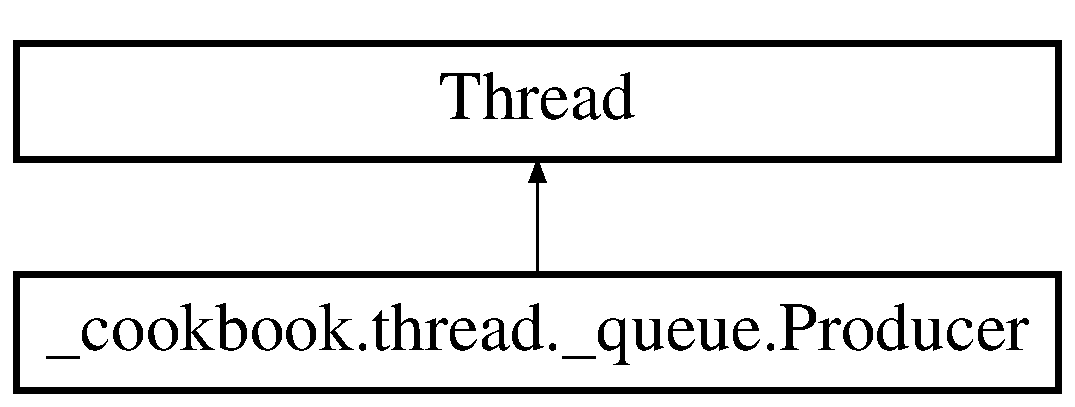
\includegraphics[height=2.000000cm]{d0/d3c/class__cookbook_1_1thread_1_1__queue_1_1Producer}
\end{center}
\end{figure}
\subsection*{Public Member Functions}
\begin{DoxyCompactItemize}
\item 
def \hyperlink{class__cookbook_1_1thread_1_1__queue_1_1Producer_a226dc5f01bf3c18175972c30a27a0aed}{\-\_\-\-\_\-init\-\_\-\-\_\-}
\item 
def \hyperlink{class__cookbook_1_1thread_1_1__queue_1_1Producer_a3ce42dbdcf7eae61b8ad89855369f7ce}{run}
\end{DoxyCompactItemize}
\subsection*{Private Attributes}
\begin{DoxyCompactItemize}
\item 
\hyperlink{class__cookbook_1_1thread_1_1__queue_1_1Producer_a685676fd503fe7d392b581506a7b3e8f}{\-\_\-times}
\item 
\hyperlink{class__cookbook_1_1thread_1_1__queue_1_1Producer_a5e71317515657aac1ad3839ab924c714}{\-\_\-item}
\end{DoxyCompactItemize}


\subsection{Detailed Description}


Definition at line 39 of file \-\_\-queue.\-py.



\subsection{Constructor \& Destructor Documentation}
\hypertarget{class__cookbook_1_1thread_1_1__queue_1_1Producer_a226dc5f01bf3c18175972c30a27a0aed}{\index{\-\_\-cookbook\-::thread\-::\-\_\-queue\-::\-Producer@{\-\_\-cookbook\-::thread\-::\-\_\-queue\-::\-Producer}!\-\_\-\-\_\-init\-\_\-\-\_\-@{\-\_\-\-\_\-init\-\_\-\-\_\-}}
\index{\-\_\-\-\_\-init\-\_\-\-\_\-@{\-\_\-\-\_\-init\-\_\-\-\_\-}!_cookbook::thread::_queue::Producer@{\-\_\-cookbook\-::thread\-::\-\_\-queue\-::\-Producer}}
\subsubsection[{\-\_\-\-\_\-init\-\_\-\-\_\-}]{\setlength{\rightskip}{0pt plus 5cm}def \-\_\-cookbook.\-thread.\-\_\-queue.\-Producer.\-\_\-\-\_\-init\-\_\-\-\_\- (
\begin{DoxyParamCaption}
\item[{}]{self, }
\item[{}]{times = {\ttfamily 1}}
\end{DoxyParamCaption}
)}}\label{class__cookbook_1_1thread_1_1__queue_1_1Producer_a226dc5f01bf3c18175972c30a27a0aed}


Definition at line 40 of file \-\_\-queue.\-py.



\subsection{Member Function Documentation}
\hypertarget{class__cookbook_1_1thread_1_1__queue_1_1Producer_a3ce42dbdcf7eae61b8ad89855369f7ce}{\index{\-\_\-cookbook\-::thread\-::\-\_\-queue\-::\-Producer@{\-\_\-cookbook\-::thread\-::\-\_\-queue\-::\-Producer}!run@{run}}
\index{run@{run}!_cookbook::thread::_queue::Producer@{\-\_\-cookbook\-::thread\-::\-\_\-queue\-::\-Producer}}
\subsubsection[{run}]{\setlength{\rightskip}{0pt plus 5cm}def \-\_\-cookbook.\-thread.\-\_\-queue.\-Producer.\-run (
\begin{DoxyParamCaption}
\item[{}]{self}
\end{DoxyParamCaption}
)}}\label{class__cookbook_1_1thread_1_1__queue_1_1Producer_a3ce42dbdcf7eae61b8ad89855369f7ce}


Definition at line 45 of file \-\_\-queue.\-py.



\subsection{Member Data Documentation}
\hypertarget{class__cookbook_1_1thread_1_1__queue_1_1Producer_a5e71317515657aac1ad3839ab924c714}{\index{\-\_\-cookbook\-::thread\-::\-\_\-queue\-::\-Producer@{\-\_\-cookbook\-::thread\-::\-\_\-queue\-::\-Producer}!\-\_\-item@{\-\_\-item}}
\index{\-\_\-item@{\-\_\-item}!_cookbook::thread::_queue::Producer@{\-\_\-cookbook\-::thread\-::\-\_\-queue\-::\-Producer}}
\subsubsection[{\-\_\-item}]{\setlength{\rightskip}{0pt plus 5cm}\-\_\-cookbook.\-thread.\-\_\-queue.\-Producer.\-\_\-item\hspace{0.3cm}{\ttfamily [private]}}}\label{class__cookbook_1_1thread_1_1__queue_1_1Producer_a5e71317515657aac1ad3839ab924c714}


Definition at line 43 of file \-\_\-queue.\-py.

\hypertarget{class__cookbook_1_1thread_1_1__queue_1_1Producer_a685676fd503fe7d392b581506a7b3e8f}{\index{\-\_\-cookbook\-::thread\-::\-\_\-queue\-::\-Producer@{\-\_\-cookbook\-::thread\-::\-\_\-queue\-::\-Producer}!\-\_\-times@{\-\_\-times}}
\index{\-\_\-times@{\-\_\-times}!_cookbook::thread::_queue::Producer@{\-\_\-cookbook\-::thread\-::\-\_\-queue\-::\-Producer}}
\subsubsection[{\-\_\-times}]{\setlength{\rightskip}{0pt plus 5cm}\-\_\-cookbook.\-thread.\-\_\-queue.\-Producer.\-\_\-times\hspace{0.3cm}{\ttfamily [private]}}}\label{class__cookbook_1_1thread_1_1__queue_1_1Producer_a685676fd503fe7d392b581506a7b3e8f}


Definition at line 42 of file \-\_\-queue.\-py.



The documentation for this class was generated from the following file\-:\begin{DoxyCompactItemize}
\item 
\-\_\-cookbook/thread/\hyperlink{__queue_8py}{\-\_\-queue.\-py}\end{DoxyCompactItemize}

\hypertarget{classadmin_1_1shell}{\section{admin.\-shell Class Reference}
\label{classadmin_1_1shell}\index{admin.\-shell@{admin.\-shell}}
}


Linux shell tools.  


Inheritance diagram for admin.\-shell\-:\begin{figure}[H]
\begin{center}
\leavevmode
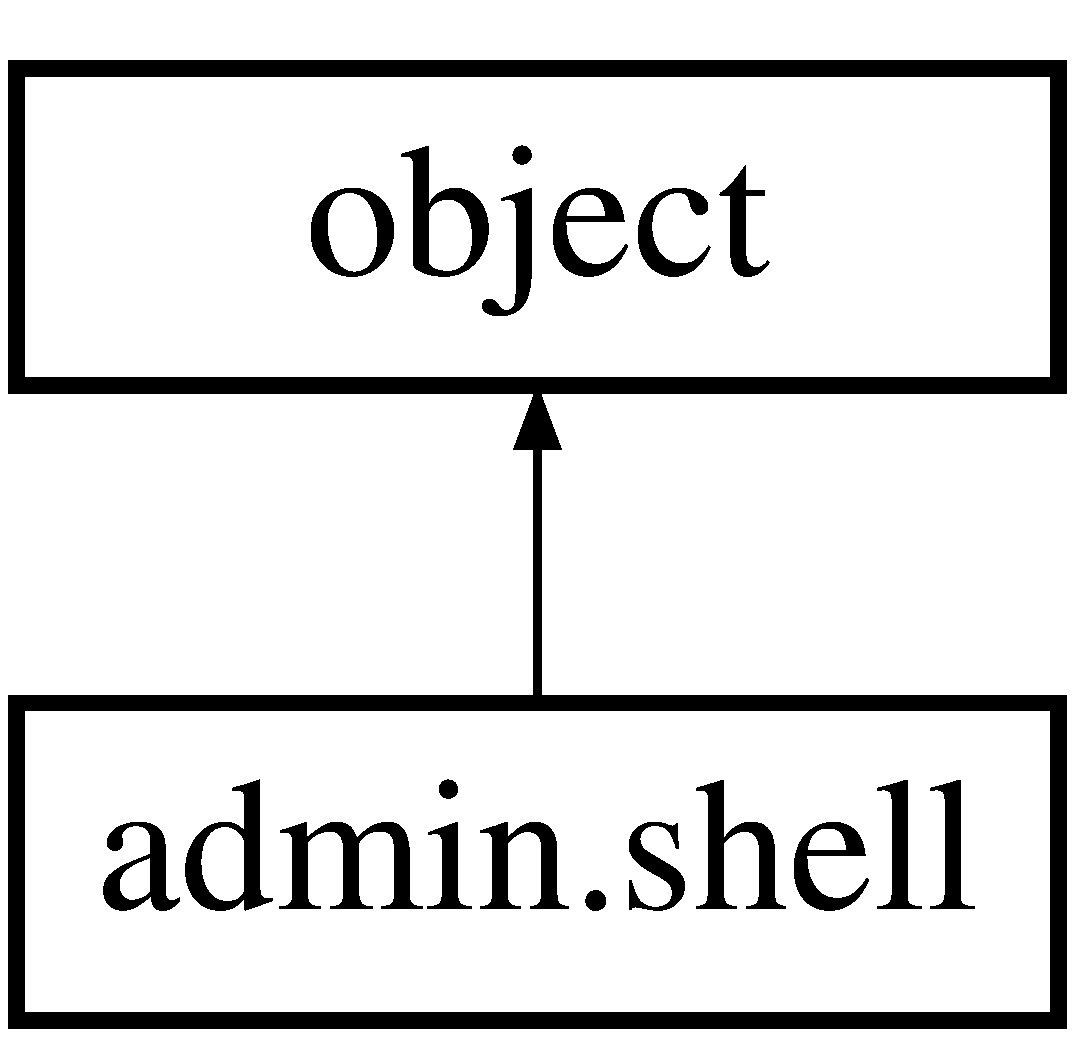
\includegraphics[height=2.000000cm]{de/d16/classadmin_1_1shell}
\end{center}
\end{figure}
\subsection*{Public Member Functions}
\begin{DoxyCompactItemize}
\item 
def \hyperlink{classadmin_1_1shell_a539012368a068a40cd347acbe49989d5}{chown}
\begin{DoxyCompactList}\small\item\em Change owner user and group of the given path. \end{DoxyCompactList}\item 
def \hyperlink{classadmin_1_1shell_ad4f8d9280283a993eec0bc5dcade6d99}{remove}
\begin{DoxyCompactList}\small\item\em Remove path entry. \end{DoxyCompactList}\item 
def \hyperlink{classadmin_1_1shell_adcdf00aa6acc1cf519ece418ce14a7f1}{mkdir}
\begin{DoxyCompactList}\small\item\em Create a directory or directories recursively. \end{DoxyCompactList}\item 
def \hyperlink{classadmin_1_1shell_a9cc97c2976b95fbcfa88b314803aa2bf}{symlink}
\begin{DoxyCompactList}\small\item\em Create a symbolic link pointing to source named {\ttfamily link\-\_\-name}. \end{DoxyCompactList}\item 
def \hyperlink{classadmin_1_1shell_a432e79bf26b0adb3e7fcf2f13f96229e}{start\-\_\-init\-\_\-service}
\begin{DoxyCompactList}\small\item\em Start init service. \end{DoxyCompactList}\item 
def \hyperlink{classadmin_1_1shell_a20ba085e92f2f4a9332d8d9c95ce7aa1}{stop\-\_\-init\-\_\-service}
\begin{DoxyCompactList}\small\item\em Stop init service. \end{DoxyCompactList}\item 
def \hyperlink{classadmin_1_1shell_ab6f38a2fae6ea2cc870c1de2d6cb6017}{restart\-\_\-init\-\_\-service}
\begin{DoxyCompactList}\small\item\em Restart init service. \end{DoxyCompactList}\end{DoxyCompactItemize}
\subsection*{Static Public Member Functions}
\begin{DoxyCompactItemize}
\item 
def \hyperlink{classadmin_1_1shell_a2ffff5c7d8eb2d2cc174df10ac1523b2}{shell}
\begin{DoxyCompactList}\small\item\em Run shell command without output. \end{DoxyCompactList}\item 
def \hyperlink{classadmin_1_1shell_a088a4609cf54f76ee4c838eea157fbc9}{read\-\_\-lines}
\begin{DoxyCompactList}\small\item\em Read specific line(s) with line number(s). \end{DoxyCompactList}\item 
def \hyperlink{classadmin_1_1shell_a5200a0188543eaaa2eb33fc295da0733}{eintr\-\_\-retry}
\begin{DoxyCompactList}\small\item\em Restart a system call interrupted by {\ttfamily E\-I\-N\-T\-R}. \end{DoxyCompactList}\item 
def \hyperlink{classadmin_1_1shell_a79f2a3efc85b54c29621697087299778}{cpu\-\_\-cores}
\end{DoxyCompactItemize}


\subsection{Detailed Description}
Linux shell tools. 

This module contains functions and classes for Linux shell, including\-:


\begin{DoxyItemize}
\item \hyperlink{classadmin_1_1shell_a2ffff5c7d8eb2d2cc174df10ac1523b2}{shell()}, \hyperlink{classadmin_1_1shell_a539012368a068a40cd347acbe49989d5}{chown()}, \hyperlink{classadmin_1_1shell_ad4f8d9280283a993eec0bc5dcade6d99}{remove()}, \hyperlink{classadmin_1_1shell_adcdf00aa6acc1cf519ece418ce14a7f1}{mkdir()}, \hyperlink{classadmin_1_1shell_a9cc97c2976b95fbcfa88b314803aa2bf}{symlink()}
\item \hyperlink{classadmin_1_1shell_a432e79bf26b0adb3e7fcf2f13f96229e}{start\-\_\-init\-\_\-service()}, \hyperlink{classadmin_1_1shell_a20ba085e92f2f4a9332d8d9c95ce7aa1}{stop\-\_\-init\-\_\-service()}, \hyperlink{classadmin_1_1shell_ab6f38a2fae6ea2cc870c1de2d6cb6017}{restart\-\_\-init\-\_\-service()}
\item \hyperlink{classadmin_1_1shell_a088a4609cf54f76ee4c838eea157fbc9}{read\-\_\-lines()}
\item \hyperlink{classadmin_1_1shell_a5200a0188543eaaa2eb33fc295da0733}{eintr\-\_\-retry()}
\item \hyperlink{classadmin_1_1shell_a79f2a3efc85b54c29621697087299778}{cpu\-\_\-cores()} (Only /proc supported system) 
\end{DoxyItemize}

Definition at line 71 of file admin.\-py.



\subsection{Constructor \& Destructor Documentation}
\hypertarget{classadmin_1_1shell_a2ffff5c7d8eb2d2cc174df10ac1523b2}{\index{admin\-::shell@{admin\-::shell}!shell@{shell}}
\index{shell@{shell}!admin::shell@{admin\-::shell}}
\subsubsection[{shell}]{\setlength{\rightskip}{0pt plus 5cm}def admin.\-shell.\-shell (
\begin{DoxyParamCaption}
\item[{}]{cmd}
\end{DoxyParamCaption}
)\hspace{0.3cm}{\ttfamily [static]}}}\label{classadmin_1_1shell_a2ffff5c7d8eb2d2cc174df10ac1523b2}


Run shell command without output. 


\begin{DoxyParams}{Parameters}
{\em cmd} & shell command \\
\hline
\end{DoxyParams}

\begin{DoxyExceptions}{Exceptions}
{\em Admin\-Error(subprocess.\-Called\-Process\-Error)} & -\/ shell command error \\
\hline
\end{DoxyExceptions}


Definition at line 78 of file admin.\-py.



\subsection{Member Function Documentation}
\hypertarget{classadmin_1_1shell_a539012368a068a40cd347acbe49989d5}{\index{admin\-::shell@{admin\-::shell}!chown@{chown}}
\index{chown@{chown}!admin::shell@{admin\-::shell}}
\subsubsection[{chown}]{\setlength{\rightskip}{0pt plus 5cm}def admin.\-shell.\-chown (
\begin{DoxyParamCaption}
\item[{}]{cls, }
\item[{}]{path, }
\item[{}]{user, }
\item[{}]{group = {\ttfamily None}}
\end{DoxyParamCaption}
)}}\label{classadmin_1_1shell_a539012368a068a40cd347acbe49989d5}


Change owner user and group of the given path. 


\begin{DoxyParams}{Parameters}
{\em path} & path whose ownership to be changed \\
\hline
{\em user} & owner user name or uid \\
\hline
{\em group} & owner group name or gid \\
\hline
\end{DoxyParams}

\begin{DoxyExceptions}{Exceptions}
{\em Admin\-Error(\-Value\-Error)} & -\/ both user or group not given \\
\hline
{\em Admin\-Error(\-Lookup\-Error)} & -\/ user or group given not in system \\
\hline
{\em Admin\-Error(subprocess.\-Called\-Process\-Error)} & -\/ shell {\ttfamily sudo chown} error \\
\hline
\end{DoxyExceptions}


Definition at line 94 of file admin.\-py.

\hypertarget{classadmin_1_1shell_a79f2a3efc85b54c29621697087299778}{\index{admin\-::shell@{admin\-::shell}!cpu\-\_\-cores@{cpu\-\_\-cores}}
\index{cpu\-\_\-cores@{cpu\-\_\-cores}!admin::shell@{admin\-::shell}}
\subsubsection[{cpu\-\_\-cores}]{\setlength{\rightskip}{0pt plus 5cm}def admin.\-shell.\-cpu\-\_\-cores (
\begin{DoxyParamCaption}
{}
\end{DoxyParamCaption}
)\hspace{0.3cm}{\ttfamily [static]}}}\label{classadmin_1_1shell_a79f2a3efc85b54c29621697087299778}


Definition at line 252 of file admin.\-py.

\hypertarget{classadmin_1_1shell_a5200a0188543eaaa2eb33fc295da0733}{\index{admin\-::shell@{admin\-::shell}!eintr\-\_\-retry@{eintr\-\_\-retry}}
\index{eintr\-\_\-retry@{eintr\-\_\-retry}!admin::shell@{admin\-::shell}}
\subsubsection[{eintr\-\_\-retry}]{\setlength{\rightskip}{0pt plus 5cm}def admin.\-shell.\-eintr\-\_\-retry (
\begin{DoxyParamCaption}
\item[{}]{func, }
\item[{}]{args}
\end{DoxyParamCaption}
)\hspace{0.3cm}{\ttfamily [static]}}}\label{classadmin_1_1shell_a5200a0188543eaaa2eb33fc295da0733}


Restart a system call interrupted by {\ttfamily E\-I\-N\-T\-R}. 


\begin{DoxyParams}{Parameters}
{\em func} & system call \\
\hline
{\em args} & arguments of system call \\
\hline
\end{DoxyParams}

\begin{DoxyExceptions}{Exceptions}
{\em socket.\-error} & -\/ socket error \\
\hline
{\em select.\-error} & -\/ select module error \\
\hline
{\em O\-S\-Error} & -\/ other O\-S errors \\
\hline
\end{DoxyExceptions}


Definition at line 238 of file admin.\-py.

\hypertarget{classadmin_1_1shell_adcdf00aa6acc1cf519ece418ce14a7f1}{\index{admin\-::shell@{admin\-::shell}!mkdir@{mkdir}}
\index{mkdir@{mkdir}!admin::shell@{admin\-::shell}}
\subsubsection[{mkdir}]{\setlength{\rightskip}{0pt plus 5cm}def admin.\-shell.\-mkdir (
\begin{DoxyParamCaption}
\item[{}]{cls, }
\item[{}]{path, }
\item[{}]{user = {\ttfamily None}, }
\item[{}]{group = {\ttfamily None}}
\end{DoxyParamCaption}
)}}\label{classadmin_1_1shell_adcdf00aa6acc1cf519ece418ce14a7f1}


Create a directory or directories recursively. 


\begin{DoxyParams}{Parameters}
{\em path} & directory path \\
\hline
{\em user} & owner user name or uid \\
\hline
{\em group} & owner group name or gid \\
\hline
\end{DoxyParams}

\begin{DoxyExceptions}{Exceptions}
{\em Admin\-Error(subprocess.\-Called\-Process\-Error)} & -\/ shell {\ttfamily sudo mkdir} error \\
\hline
{\em Admin\-Error(\-Value\-Error)} & -\/ both user or group not given \\
\hline
{\em Admin\-Error(\-Lookup\-Error)} & -\/ user or group given not in system \\
\hline
{\em Admin\-Error(subprocess.\-Called\-Process\-Error)} & -\/ change ownership error\\
\hline
\end{DoxyExceptions}
\begin{DoxySince}{Since}
Python 3.\-2 
\end{DoxySince}


Definition at line 156 of file admin.\-py.

\hypertarget{classadmin_1_1shell_a088a4609cf54f76ee4c838eea157fbc9}{\index{admin\-::shell@{admin\-::shell}!read\-\_\-lines@{read\-\_\-lines}}
\index{read\-\_\-lines@{read\-\_\-lines}!admin::shell@{admin\-::shell}}
\subsubsection[{read\-\_\-lines}]{\setlength{\rightskip}{0pt plus 5cm}def admin.\-shell.\-read\-\_\-lines (
\begin{DoxyParamCaption}
\item[{}]{filename, }
\item[{}]{lineno}
\end{DoxyParamCaption}
)\hspace{0.3cm}{\ttfamily [static]}}}\label{classadmin_1_1shell_a088a4609cf54f76ee4c838eea157fbc9}


Read specific line(s) with line number(s). 


\begin{DoxyParams}{Parameters}
{\em filename} & file name \\
\hline
{\em lineno} & line number(s) to read (starting with 1) \\
\hline
\end{DoxyParams}
\begin{DoxyReturn}{Returns}
generator object of line with no terminating line break 
\end{DoxyReturn}

\begin{DoxyExceptions}{Exceptions}
{\em Type\-Error,I\-O\-Error} & \\
\hline
\end{DoxyExceptions}


Definition at line 217 of file admin.\-py.

\hypertarget{classadmin_1_1shell_ad4f8d9280283a993eec0bc5dcade6d99}{\index{admin\-::shell@{admin\-::shell}!remove@{remove}}
\index{remove@{remove}!admin::shell@{admin\-::shell}}
\subsubsection[{remove}]{\setlength{\rightskip}{0pt plus 5cm}def admin.\-shell.\-remove (
\begin{DoxyParamCaption}
\item[{}]{cls, }
\item[{}]{path}
\end{DoxyParamCaption}
)}}\label{classadmin_1_1shell_ad4f8d9280283a993eec0bc5dcade6d99}


Remove path entry. 


\begin{DoxyParams}{Parameters}
{\em path} & path name of entry to be removed \\
\hline
\end{DoxyParams}

\begin{DoxyExceptions}{Exceptions}
{\em Admin\-Error(subprocess.\-Called\-Process\-Error)} & -\/ shell 'sudo rm -\/f' error \\
\hline
\end{DoxyExceptions}


Definition at line 125 of file admin.\-py.

\hypertarget{classadmin_1_1shell_ab6f38a2fae6ea2cc870c1de2d6cb6017}{\index{admin\-::shell@{admin\-::shell}!restart\-\_\-init\-\_\-service@{restart\-\_\-init\-\_\-service}}
\index{restart\-\_\-init\-\_\-service@{restart\-\_\-init\-\_\-service}!admin::shell@{admin\-::shell}}
\subsubsection[{restart\-\_\-init\-\_\-service}]{\setlength{\rightskip}{0pt plus 5cm}def admin.\-shell.\-restart\-\_\-init\-\_\-service (
\begin{DoxyParamCaption}
\item[{}]{cls, }
\item[{}]{service}
\end{DoxyParamCaption}
)}}\label{classadmin_1_1shell_ab6f38a2fae6ea2cc870c1de2d6cb6017}


Restart init service. 


\begin{DoxyParams}{Parameters}
{\em service} & service name \\
\hline
\end{DoxyParams}

\begin{DoxyExceptions}{Exceptions}
{\em Admin\-Error(subprocess.\-Called\-Process\-Error)} & -\/ shell {\ttfamily sudo /etc/init.d} error \\
\hline
\end{DoxyExceptions}


Definition at line 206 of file admin.\-py.

\hypertarget{classadmin_1_1shell_a432e79bf26b0adb3e7fcf2f13f96229e}{\index{admin\-::shell@{admin\-::shell}!start\-\_\-init\-\_\-service@{start\-\_\-init\-\_\-service}}
\index{start\-\_\-init\-\_\-service@{start\-\_\-init\-\_\-service}!admin::shell@{admin\-::shell}}
\subsubsection[{start\-\_\-init\-\_\-service}]{\setlength{\rightskip}{0pt plus 5cm}def admin.\-shell.\-start\-\_\-init\-\_\-service (
\begin{DoxyParamCaption}
\item[{}]{cls, }
\item[{}]{service}
\end{DoxyParamCaption}
)}}\label{classadmin_1_1shell_a432e79bf26b0adb3e7fcf2f13f96229e}


Start init service. 


\begin{DoxyParams}{Parameters}
{\em service} & service name \\
\hline
\end{DoxyParams}

\begin{DoxyExceptions}{Exceptions}
{\em Admin\-Error(subprocess.\-Called\-Process\-Error)} & -\/ shell {\ttfamily sudo /etc/init.d} error \\
\hline
\end{DoxyExceptions}


Definition at line 188 of file admin.\-py.

\hypertarget{classadmin_1_1shell_a20ba085e92f2f4a9332d8d9c95ce7aa1}{\index{admin\-::shell@{admin\-::shell}!stop\-\_\-init\-\_\-service@{stop\-\_\-init\-\_\-service}}
\index{stop\-\_\-init\-\_\-service@{stop\-\_\-init\-\_\-service}!admin::shell@{admin\-::shell}}
\subsubsection[{stop\-\_\-init\-\_\-service}]{\setlength{\rightskip}{0pt plus 5cm}def admin.\-shell.\-stop\-\_\-init\-\_\-service (
\begin{DoxyParamCaption}
\item[{}]{cls, }
\item[{}]{service}
\end{DoxyParamCaption}
)}}\label{classadmin_1_1shell_a20ba085e92f2f4a9332d8d9c95ce7aa1}


Stop init service. 


\begin{DoxyParams}{Parameters}
{\em service} & service name \\
\hline
\end{DoxyParams}

\begin{DoxyExceptions}{Exceptions}
{\em Admin\-Error(subprocess.\-Called\-Process\-Error)} & -\/ shell {\ttfamily sudo /etc/init.d} error \\
\hline
\end{DoxyExceptions}


Definition at line 197 of file admin.\-py.

\hypertarget{classadmin_1_1shell_a9cc97c2976b95fbcfa88b314803aa2bf}{\index{admin\-::shell@{admin\-::shell}!symlink@{symlink}}
\index{symlink@{symlink}!admin::shell@{admin\-::shell}}
\subsubsection[{symlink}]{\setlength{\rightskip}{0pt plus 5cm}def admin.\-shell.\-symlink (
\begin{DoxyParamCaption}
\item[{}]{cls, }
\item[{}]{src, }
\item[{}]{link\-\_\-name}
\end{DoxyParamCaption}
)}}\label{classadmin_1_1shell_a9cc97c2976b95fbcfa88b314803aa2bf}


Create a symbolic link pointing to source named {\ttfamily link\-\_\-name}. 


\begin{DoxyParams}{Parameters}
{\em src} & source file \\
\hline
{\em link\-\_\-name} & symbolic link name \\
\hline
\end{DoxyParams}

\begin{DoxyExceptions}{Exceptions}
{\em Admin\-Error(subprocess.\-Called\-Process\-Error)} & -\/ shell {\ttfamily sudo ln -\/sf} error \\
\hline
\end{DoxyExceptions}


Definition at line 173 of file admin.\-py.



The documentation for this class was generated from the following file\-:\begin{DoxyCompactItemize}
\item 
\hyperlink{admin_8py}{admin.\-py}\end{DoxyCompactItemize}

\hypertarget{class__cookbook_1_1my__pyunit_1_1TestCase}{\section{\-\_\-cookbook.\-my\-\_\-pyunit.\-Test\-Case Class Reference}
\label{class__cookbook_1_1my__pyunit_1_1TestCase}\index{\-\_\-cookbook.\-my\-\_\-pyunit.\-Test\-Case@{\-\_\-cookbook.\-my\-\_\-pyunit.\-Test\-Case}}
}
Inheritance diagram for \-\_\-cookbook.\-my\-\_\-pyunit.\-Test\-Case\-:\begin{figure}[H]
\begin{center}
\leavevmode
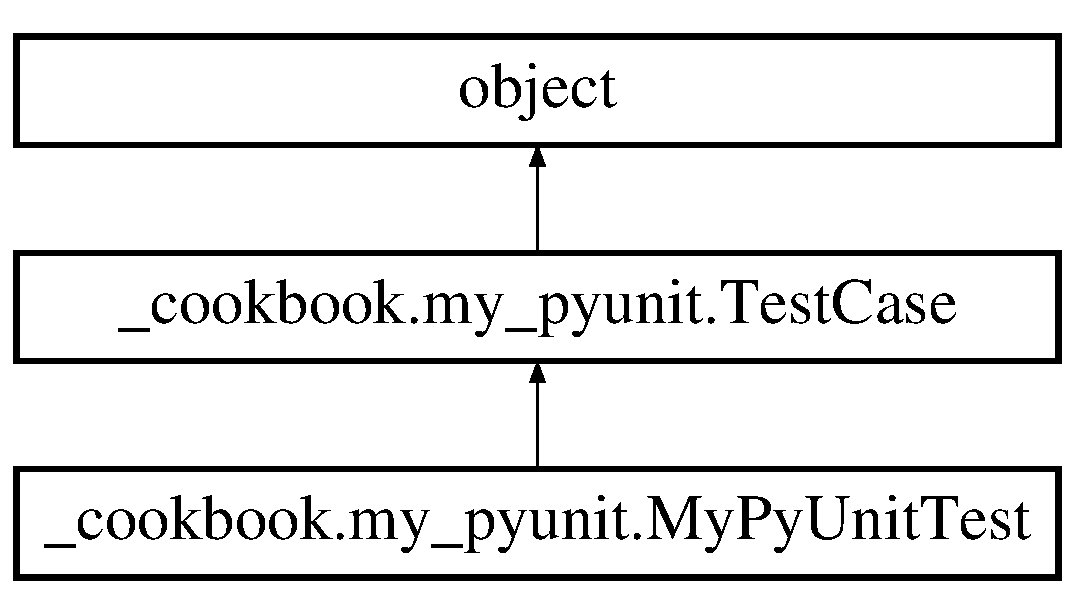
\includegraphics[height=3.000000cm]{d5/d0e/class__cookbook_1_1my__pyunit_1_1TestCase}
\end{center}
\end{figure}
\subsection*{Public Member Functions}
\begin{DoxyCompactItemize}
\item 
def \hyperlink{class__cookbook_1_1my__pyunit_1_1TestCase_aba31c6c59f32b40e390fbeb4a00a4e87}{\-\_\-\-\_\-init\-\_\-\-\_\-}
\item 
def \hyperlink{class__cookbook_1_1my__pyunit_1_1TestCase_a9af9fafdc8f337109d08db63ebd18fd2}{set\-Up}
\item 
def \hyperlink{class__cookbook_1_1my__pyunit_1_1TestCase_ab77325c9f2ce70b345883d56c1f86872}{tear\-Down}
\item 
def \hyperlink{class__cookbook_1_1my__pyunit_1_1TestCase_af0e73c2611cd4bdcff403ef50befc044}{run}
\item 
def \hyperlink{class__cookbook_1_1my__pyunit_1_1TestCase_a12cc1032e4ad38c28767de95adcffd0e}{summary}
\item 
def \hyperlink{class__cookbook_1_1my__pyunit_1_1TestCase_a882b78923fece4ed2e93abdf28a759fc}{assert\-True}
\item 
def \hyperlink{class__cookbook_1_1my__pyunit_1_1TestCase_a9e0dcc921b9d184ea7ed32b729ff4362}{assert\-Equal}
\item 
def \hyperlink{class__cookbook_1_1my__pyunit_1_1TestCase_a1a6e6cfc473a84cf431cd262bce94c82}{assert\-Greater}
\item 
def \hyperlink{class__cookbook_1_1my__pyunit_1_1TestCase_a9542fc7ac24ec1e1c4163f135c753f84}{assert\-Less}
\item 
def \hyperlink{class__cookbook_1_1my__pyunit_1_1TestCase_ad3acee5c46f3b10f8d78125aa5e8c8b9}{assert\-Greater\-Equal}
\item 
def \hyperlink{class__cookbook_1_1my__pyunit_1_1TestCase_a91c192bb291d88a5b2a13df6da661217}{assert\-Less\-Equal}
\end{DoxyCompactItemize}
\subsection*{Public Attributes}
\begin{DoxyCompactItemize}
\item 
\hyperlink{class__cookbook_1_1my__pyunit_1_1TestCase_a5fa4c4edcd81210291d7afa3c82321e3}{tests}
\item 
\hyperlink{class__cookbook_1_1my__pyunit_1_1TestCase_a6bef30a7e15e97ea3e0516dd58517dd7}{errors}
\end{DoxyCompactItemize}


\subsection{Detailed Description}
\begin{DoxyVerb}A class whose instances are single test cases.

If the fixture may be used for many test cases, create as
many test methods as are needed. When instantiating such a TestCase
subclass, specify in the constructor arguments the name of the test method
that the instance is to execute.

Test authors should subclass TestCase for their own tests. Construction
and clean up of the test's environment ('fixture') can be implemented
by overriding the 'setUp' and 'tearDown' methods respectively.

If it is necessary to override the __init__ method, the base class
__init__ method must always be called. It is important that subclasses
should not change the signature of their __init__ method, since instances
of the classes are instantiated automatically by parts of the framework
in order to be run.
\end{DoxyVerb}
 

Definition at line 60 of file my\-\_\-pyunit.\-py.



\subsection{Constructor \& Destructor Documentation}
\hypertarget{class__cookbook_1_1my__pyunit_1_1TestCase_aba31c6c59f32b40e390fbeb4a00a4e87}{\index{\-\_\-cookbook\-::my\-\_\-pyunit\-::\-Test\-Case@{\-\_\-cookbook\-::my\-\_\-pyunit\-::\-Test\-Case}!\-\_\-\-\_\-init\-\_\-\-\_\-@{\-\_\-\-\_\-init\-\_\-\-\_\-}}
\index{\-\_\-\-\_\-init\-\_\-\-\_\-@{\-\_\-\-\_\-init\-\_\-\-\_\-}!_cookbook::my_pyunit::TestCase@{\-\_\-cookbook\-::my\-\_\-pyunit\-::\-Test\-Case}}
\subsubsection[{\-\_\-\-\_\-init\-\_\-\-\_\-}]{\setlength{\rightskip}{0pt plus 5cm}def \-\_\-cookbook.\-my\-\_\-pyunit.\-Test\-Case.\-\_\-\-\_\-init\-\_\-\-\_\- (
\begin{DoxyParamCaption}
\item[{}]{self}
\end{DoxyParamCaption}
)}}\label{class__cookbook_1_1my__pyunit_1_1TestCase_aba31c6c59f32b40e390fbeb4a00a4e87}


Definition at line 78 of file my\-\_\-pyunit.\-py.



\subsection{Member Function Documentation}
\hypertarget{class__cookbook_1_1my__pyunit_1_1TestCase_a9e0dcc921b9d184ea7ed32b729ff4362}{\index{\-\_\-cookbook\-::my\-\_\-pyunit\-::\-Test\-Case@{\-\_\-cookbook\-::my\-\_\-pyunit\-::\-Test\-Case}!assert\-Equal@{assert\-Equal}}
\index{assert\-Equal@{assert\-Equal}!_cookbook::my_pyunit::TestCase@{\-\_\-cookbook\-::my\-\_\-pyunit\-::\-Test\-Case}}
\subsubsection[{assert\-Equal}]{\setlength{\rightskip}{0pt plus 5cm}def \-\_\-cookbook.\-my\-\_\-pyunit.\-Test\-Case.\-assert\-Equal (
\begin{DoxyParamCaption}
\item[{}]{self, }
\item[{}]{obj1, }
\item[{}]{obj2}
\end{DoxyParamCaption}
)}}\label{class__cookbook_1_1my__pyunit_1_1TestCase_a9e0dcc921b9d184ea7ed32b729ff4362}
\begin{DoxyVerb}Check that the two given objects are equal.

@param obj1 The first checked object.
@param obj2 The second checked object.
\end{DoxyVerb}
 

Definition at line 134 of file my\-\_\-pyunit.\-py.

\hypertarget{class__cookbook_1_1my__pyunit_1_1TestCase_a1a6e6cfc473a84cf431cd262bce94c82}{\index{\-\_\-cookbook\-::my\-\_\-pyunit\-::\-Test\-Case@{\-\_\-cookbook\-::my\-\_\-pyunit\-::\-Test\-Case}!assert\-Greater@{assert\-Greater}}
\index{assert\-Greater@{assert\-Greater}!_cookbook::my_pyunit::TestCase@{\-\_\-cookbook\-::my\-\_\-pyunit\-::\-Test\-Case}}
\subsubsection[{assert\-Greater}]{\setlength{\rightskip}{0pt plus 5cm}def \-\_\-cookbook.\-my\-\_\-pyunit.\-Test\-Case.\-assert\-Greater (
\begin{DoxyParamCaption}
\item[{}]{self, }
\item[{}]{obj1, }
\item[{}]{obj2}
\end{DoxyParamCaption}
)}}\label{class__cookbook_1_1my__pyunit_1_1TestCase_a1a6e6cfc473a84cf431cd262bce94c82}
\begin{DoxyVerb}Check that the first given object is greater than the second one.

@param obj1 The first checked object.
@param obj2 The second checked object.
\end{DoxyVerb}
 

Definition at line 143 of file my\-\_\-pyunit.\-py.

\hypertarget{class__cookbook_1_1my__pyunit_1_1TestCase_ad3acee5c46f3b10f8d78125aa5e8c8b9}{\index{\-\_\-cookbook\-::my\-\_\-pyunit\-::\-Test\-Case@{\-\_\-cookbook\-::my\-\_\-pyunit\-::\-Test\-Case}!assert\-Greater\-Equal@{assert\-Greater\-Equal}}
\index{assert\-Greater\-Equal@{assert\-Greater\-Equal}!_cookbook::my_pyunit::TestCase@{\-\_\-cookbook\-::my\-\_\-pyunit\-::\-Test\-Case}}
\subsubsection[{assert\-Greater\-Equal}]{\setlength{\rightskip}{0pt plus 5cm}def \-\_\-cookbook.\-my\-\_\-pyunit.\-Test\-Case.\-assert\-Greater\-Equal (
\begin{DoxyParamCaption}
\item[{}]{self, }
\item[{}]{obj1, }
\item[{}]{obj2}
\end{DoxyParamCaption}
)}}\label{class__cookbook_1_1my__pyunit_1_1TestCase_ad3acee5c46f3b10f8d78125aa5e8c8b9}
\begin{DoxyVerb}Check that the first given object is greater than or equals to the
second one.

@param obj1 The first checked object.
@param obj2 The second checked object.
\end{DoxyVerb}
 

Definition at line 161 of file my\-\_\-pyunit.\-py.

\hypertarget{class__cookbook_1_1my__pyunit_1_1TestCase_a9542fc7ac24ec1e1c4163f135c753f84}{\index{\-\_\-cookbook\-::my\-\_\-pyunit\-::\-Test\-Case@{\-\_\-cookbook\-::my\-\_\-pyunit\-::\-Test\-Case}!assert\-Less@{assert\-Less}}
\index{assert\-Less@{assert\-Less}!_cookbook::my_pyunit::TestCase@{\-\_\-cookbook\-::my\-\_\-pyunit\-::\-Test\-Case}}
\subsubsection[{assert\-Less}]{\setlength{\rightskip}{0pt plus 5cm}def \-\_\-cookbook.\-my\-\_\-pyunit.\-Test\-Case.\-assert\-Less (
\begin{DoxyParamCaption}
\item[{}]{self, }
\item[{}]{obj1, }
\item[{}]{obj2}
\end{DoxyParamCaption}
)}}\label{class__cookbook_1_1my__pyunit_1_1TestCase_a9542fc7ac24ec1e1c4163f135c753f84}
\begin{DoxyVerb}Check that the first given object is less than the second one.

@param obj1 The first checked object.
@param obj2 The second checked object.
\end{DoxyVerb}
 

Definition at line 152 of file my\-\_\-pyunit.\-py.

\hypertarget{class__cookbook_1_1my__pyunit_1_1TestCase_a91c192bb291d88a5b2a13df6da661217}{\index{\-\_\-cookbook\-::my\-\_\-pyunit\-::\-Test\-Case@{\-\_\-cookbook\-::my\-\_\-pyunit\-::\-Test\-Case}!assert\-Less\-Equal@{assert\-Less\-Equal}}
\index{assert\-Less\-Equal@{assert\-Less\-Equal}!_cookbook::my_pyunit::TestCase@{\-\_\-cookbook\-::my\-\_\-pyunit\-::\-Test\-Case}}
\subsubsection[{assert\-Less\-Equal}]{\setlength{\rightskip}{0pt plus 5cm}def \-\_\-cookbook.\-my\-\_\-pyunit.\-Test\-Case.\-assert\-Less\-Equal (
\begin{DoxyParamCaption}
\item[{}]{self, }
\item[{}]{obj1, }
\item[{}]{obj2}
\end{DoxyParamCaption}
)}}\label{class__cookbook_1_1my__pyunit_1_1TestCase_a91c192bb291d88a5b2a13df6da661217}
\begin{DoxyVerb}Check that the first given object is less than or equals to the
second one.

@param obj1 The first checked object.
@param obj2 The second checked object.
\end{DoxyVerb}
 

Definition at line 171 of file my\-\_\-pyunit.\-py.

\hypertarget{class__cookbook_1_1my__pyunit_1_1TestCase_a882b78923fece4ed2e93abdf28a759fc}{\index{\-\_\-cookbook\-::my\-\_\-pyunit\-::\-Test\-Case@{\-\_\-cookbook\-::my\-\_\-pyunit\-::\-Test\-Case}!assert\-True@{assert\-True}}
\index{assert\-True@{assert\-True}!_cookbook::my_pyunit::TestCase@{\-\_\-cookbook\-::my\-\_\-pyunit\-::\-Test\-Case}}
\subsubsection[{assert\-True}]{\setlength{\rightskip}{0pt plus 5cm}def \-\_\-cookbook.\-my\-\_\-pyunit.\-Test\-Case.\-assert\-True (
\begin{DoxyParamCaption}
\item[{}]{self, }
\item[{}]{exp}
\end{DoxyParamCaption}
)}}\label{class__cookbook_1_1my__pyunit_1_1TestCase_a882b78923fece4ed2e93abdf28a759fc}
\begin{DoxyVerb}Check that the expression is true.

@param exp Expression to be checked.
\end{DoxyVerb}
 

Definition at line 125 of file my\-\_\-pyunit.\-py.

\hypertarget{class__cookbook_1_1my__pyunit_1_1TestCase_af0e73c2611cd4bdcff403ef50befc044}{\index{\-\_\-cookbook\-::my\-\_\-pyunit\-::\-Test\-Case@{\-\_\-cookbook\-::my\-\_\-pyunit\-::\-Test\-Case}!run@{run}}
\index{run@{run}!_cookbook::my_pyunit::TestCase@{\-\_\-cookbook\-::my\-\_\-pyunit\-::\-Test\-Case}}
\subsubsection[{run}]{\setlength{\rightskip}{0pt plus 5cm}def \-\_\-cookbook.\-my\-\_\-pyunit.\-Test\-Case.\-run (
\begin{DoxyParamCaption}
\item[{}]{self}
\end{DoxyParamCaption}
)}}\label{class__cookbook_1_1my__pyunit_1_1TestCase_af0e73c2611cd4bdcff403ef50befc044}


Definition at line 101 of file my\-\_\-pyunit.\-py.

\hypertarget{class__cookbook_1_1my__pyunit_1_1TestCase_a9af9fafdc8f337109d08db63ebd18fd2}{\index{\-\_\-cookbook\-::my\-\_\-pyunit\-::\-Test\-Case@{\-\_\-cookbook\-::my\-\_\-pyunit\-::\-Test\-Case}!set\-Up@{set\-Up}}
\index{set\-Up@{set\-Up}!_cookbook::my_pyunit::TestCase@{\-\_\-cookbook\-::my\-\_\-pyunit\-::\-Test\-Case}}
\subsubsection[{set\-Up}]{\setlength{\rightskip}{0pt plus 5cm}def \-\_\-cookbook.\-my\-\_\-pyunit.\-Test\-Case.\-set\-Up (
\begin{DoxyParamCaption}
\item[{}]{self}
\end{DoxyParamCaption}
)}}\label{class__cookbook_1_1my__pyunit_1_1TestCase_a9af9fafdc8f337109d08db63ebd18fd2}
\begin{DoxyVerb}Hook method for setting up the test fixture before exercising it.

Test authors should override this method in the subclass of TestCase
to construct the test's environment ('fixture') respectively.
\end{DoxyVerb}
 

Definition at line 83 of file my\-\_\-pyunit.\-py.

\hypertarget{class__cookbook_1_1my__pyunit_1_1TestCase_a12cc1032e4ad38c28767de95adcffd0e}{\index{\-\_\-cookbook\-::my\-\_\-pyunit\-::\-Test\-Case@{\-\_\-cookbook\-::my\-\_\-pyunit\-::\-Test\-Case}!summary@{summary}}
\index{summary@{summary}!_cookbook::my_pyunit::TestCase@{\-\_\-cookbook\-::my\-\_\-pyunit\-::\-Test\-Case}}
\subsubsection[{summary}]{\setlength{\rightskip}{0pt plus 5cm}def \-\_\-cookbook.\-my\-\_\-pyunit.\-Test\-Case.\-summary (
\begin{DoxyParamCaption}
\item[{}]{self}
\end{DoxyParamCaption}
)}}\label{class__cookbook_1_1my__pyunit_1_1TestCase_a12cc1032e4ad38c28767de95adcffd0e}
\begin{DoxyVerb}Returns a summary of the testing report, that includes information
of the number of test cases being run and how many failed cases
occur.

@return String of testing report summary.
\end{DoxyVerb}
 

Definition at line 114 of file my\-\_\-pyunit.\-py.

\hypertarget{class__cookbook_1_1my__pyunit_1_1TestCase_ab77325c9f2ce70b345883d56c1f86872}{\index{\-\_\-cookbook\-::my\-\_\-pyunit\-::\-Test\-Case@{\-\_\-cookbook\-::my\-\_\-pyunit\-::\-Test\-Case}!tear\-Down@{tear\-Down}}
\index{tear\-Down@{tear\-Down}!_cookbook::my_pyunit::TestCase@{\-\_\-cookbook\-::my\-\_\-pyunit\-::\-Test\-Case}}
\subsubsection[{tear\-Down}]{\setlength{\rightskip}{0pt plus 5cm}def \-\_\-cookbook.\-my\-\_\-pyunit.\-Test\-Case.\-tear\-Down (
\begin{DoxyParamCaption}
\item[{}]{self}
\end{DoxyParamCaption}
)}}\label{class__cookbook_1_1my__pyunit_1_1TestCase_ab77325c9f2ce70b345883d56c1f86872}
\begin{DoxyVerb}Hook method for cleaning up the test fixture after testing it.

Test authors should override this method in the subclass of TestCase
to clean up the test's environment ('fixture') respectively.
\end{DoxyVerb}
 

Definition at line 92 of file my\-\_\-pyunit.\-py.



\subsection{Member Data Documentation}
\hypertarget{class__cookbook_1_1my__pyunit_1_1TestCase_a6bef30a7e15e97ea3e0516dd58517dd7}{\index{\-\_\-cookbook\-::my\-\_\-pyunit\-::\-Test\-Case@{\-\_\-cookbook\-::my\-\_\-pyunit\-::\-Test\-Case}!errors@{errors}}
\index{errors@{errors}!_cookbook::my_pyunit::TestCase@{\-\_\-cookbook\-::my\-\_\-pyunit\-::\-Test\-Case}}
\subsubsection[{errors}]{\setlength{\rightskip}{0pt plus 5cm}\-\_\-cookbook.\-my\-\_\-pyunit.\-Test\-Case.\-errors}}\label{class__cookbook_1_1my__pyunit_1_1TestCase_a6bef30a7e15e97ea3e0516dd58517dd7}


Definition at line 80 of file my\-\_\-pyunit.\-py.

\hypertarget{class__cookbook_1_1my__pyunit_1_1TestCase_a5fa4c4edcd81210291d7afa3c82321e3}{\index{\-\_\-cookbook\-::my\-\_\-pyunit\-::\-Test\-Case@{\-\_\-cookbook\-::my\-\_\-pyunit\-::\-Test\-Case}!tests@{tests}}
\index{tests@{tests}!_cookbook::my_pyunit::TestCase@{\-\_\-cookbook\-::my\-\_\-pyunit\-::\-Test\-Case}}
\subsubsection[{tests}]{\setlength{\rightskip}{0pt plus 5cm}\-\_\-cookbook.\-my\-\_\-pyunit.\-Test\-Case.\-tests}}\label{class__cookbook_1_1my__pyunit_1_1TestCase_a5fa4c4edcd81210291d7afa3c82321e3}


Definition at line 79 of file my\-\_\-pyunit.\-py.



The documentation for this class was generated from the following file\-:\begin{DoxyCompactItemize}
\item 
\-\_\-cookbook/\hyperlink{my__pyunit_8py}{my\-\_\-pyunit.\-py}\end{DoxyCompactItemize}

\hypertarget{class__cookbook_1_1my__pyunit_1_1TestSuite}{\section{\-\_\-cookbook.\-my\-\_\-pyunit.\-Test\-Suite Class Reference}
\label{class__cookbook_1_1my__pyunit_1_1TestSuite}\index{\-\_\-cookbook.\-my\-\_\-pyunit.\-Test\-Suite@{\-\_\-cookbook.\-my\-\_\-pyunit.\-Test\-Suite}}
}
Inheritance diagram for \-\_\-cookbook.\-my\-\_\-pyunit.\-Test\-Suite\-:\begin{figure}[H]
\begin{center}
\leavevmode
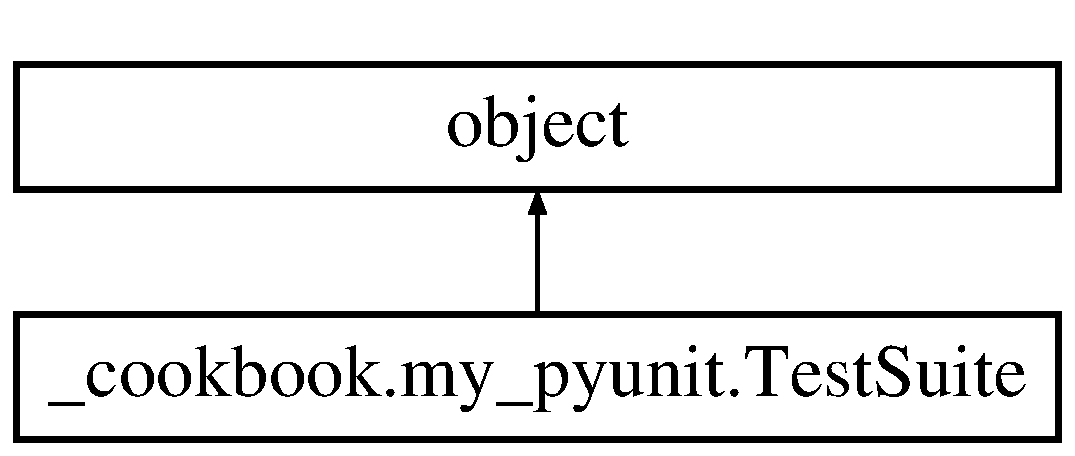
\includegraphics[height=2.000000cm]{df/def/class__cookbook_1_1my__pyunit_1_1TestSuite}
\end{center}
\end{figure}
\subsection*{Public Member Functions}
\begin{DoxyCompactItemize}
\item 
def \hyperlink{class__cookbook_1_1my__pyunit_1_1TestSuite_a9ac8bc8c1f00434b0a16985762c3bc30}{\-\_\-\-\_\-init\-\_\-\-\_\-}
\item 
def \hyperlink{class__cookbook_1_1my__pyunit_1_1TestSuite_af7fc14f84559e4ac099b3a991f4fe077}{add\-Test\-Case}
\item 
def \hyperlink{class__cookbook_1_1my__pyunit_1_1TestSuite_a246a14a895b60b1765e1a4da7c16191a}{add\-Test\-Case\-From\-Class}
\item 
def \hyperlink{class__cookbook_1_1my__pyunit_1_1TestSuite_a0dc0859f477dc0c3d564f2148cdbba1c}{run}
\end{DoxyCompactItemize}
\subsection*{Public Attributes}
\begin{DoxyCompactItemize}
\item 
\hyperlink{class__cookbook_1_1my__pyunit_1_1TestSuite_aa72351c9916112e29864390633a480a0}{suite}
\end{DoxyCompactItemize}


\subsection{Detailed Description}
\begin{DoxyVerb}A test suite is a composite test consisting of a number of TestCases.

For use, create an instance of TestSuite, then add test case instances.
When all tests have been added, the suite can be passed to a test
runner, such as run(). It will run the individual test cases
in the order in which they were added, aggregating the results. When
subclassing, do not forget to call the base class constructor.
\end{DoxyVerb}
 

Definition at line 181 of file my\-\_\-pyunit.\-py.



\subsection{Constructor \& Destructor Documentation}
\hypertarget{class__cookbook_1_1my__pyunit_1_1TestSuite_a9ac8bc8c1f00434b0a16985762c3bc30}{\index{\-\_\-cookbook\-::my\-\_\-pyunit\-::\-Test\-Suite@{\-\_\-cookbook\-::my\-\_\-pyunit\-::\-Test\-Suite}!\-\_\-\-\_\-init\-\_\-\-\_\-@{\-\_\-\-\_\-init\-\_\-\-\_\-}}
\index{\-\_\-\-\_\-init\-\_\-\-\_\-@{\-\_\-\-\_\-init\-\_\-\-\_\-}!_cookbook::my_pyunit::TestSuite@{\-\_\-cookbook\-::my\-\_\-pyunit\-::\-Test\-Suite}}
\subsubsection[{\-\_\-\-\_\-init\-\_\-\-\_\-}]{\setlength{\rightskip}{0pt plus 5cm}def \-\_\-cookbook.\-my\-\_\-pyunit.\-Test\-Suite.\-\_\-\-\_\-init\-\_\-\-\_\- (
\begin{DoxyParamCaption}
\item[{}]{self}
\end{DoxyParamCaption}
)}}\label{class__cookbook_1_1my__pyunit_1_1TestSuite_a9ac8bc8c1f00434b0a16985762c3bc30}


Definition at line 190 of file my\-\_\-pyunit.\-py.



\subsection{Member Function Documentation}
\hypertarget{class__cookbook_1_1my__pyunit_1_1TestSuite_af7fc14f84559e4ac099b3a991f4fe077}{\index{\-\_\-cookbook\-::my\-\_\-pyunit\-::\-Test\-Suite@{\-\_\-cookbook\-::my\-\_\-pyunit\-::\-Test\-Suite}!add\-Test\-Case@{add\-Test\-Case}}
\index{add\-Test\-Case@{add\-Test\-Case}!_cookbook::my_pyunit::TestSuite@{\-\_\-cookbook\-::my\-\_\-pyunit\-::\-Test\-Suite}}
\subsubsection[{add\-Test\-Case}]{\setlength{\rightskip}{0pt plus 5cm}def \-\_\-cookbook.\-my\-\_\-pyunit.\-Test\-Suite.\-add\-Test\-Case (
\begin{DoxyParamCaption}
\item[{}]{self, }
\item[{}]{test\-\_\-case}
\end{DoxyParamCaption}
)}}\label{class__cookbook_1_1my__pyunit_1_1TestSuite_af7fc14f84559e4ac099b3a991f4fe077}
\begin{DoxyVerb}Add test case instance.

If the given object is not the instance of TestCase, nothing to be
done.

@param test_case test case instance that is added.
\end{DoxyVerb}
 

Definition at line 194 of file my\-\_\-pyunit.\-py.

\hypertarget{class__cookbook_1_1my__pyunit_1_1TestSuite_a246a14a895b60b1765e1a4da7c16191a}{\index{\-\_\-cookbook\-::my\-\_\-pyunit\-::\-Test\-Suite@{\-\_\-cookbook\-::my\-\_\-pyunit\-::\-Test\-Suite}!add\-Test\-Case\-From\-Class@{add\-Test\-Case\-From\-Class}}
\index{add\-Test\-Case\-From\-Class@{add\-Test\-Case\-From\-Class}!_cookbook::my_pyunit::TestSuite@{\-\_\-cookbook\-::my\-\_\-pyunit\-::\-Test\-Suite}}
\subsubsection[{add\-Test\-Case\-From\-Class}]{\setlength{\rightskip}{0pt plus 5cm}def \-\_\-cookbook.\-my\-\_\-pyunit.\-Test\-Suite.\-add\-Test\-Case\-From\-Class (
\begin{DoxyParamCaption}
\item[{}]{self, }
\item[{}]{test\-\_\-case}
\end{DoxyParamCaption}
)}}\label{class__cookbook_1_1my__pyunit_1_1TestSuite_a246a14a895b60b1765e1a4da7c16191a}
\begin{DoxyVerb}Add test case.

If the given class is not the subclass of the TestCase, nothing to be
done.

@param test_case class of test case that is added.
\end{DoxyVerb}
 

Definition at line 206 of file my\-\_\-pyunit.\-py.

\hypertarget{class__cookbook_1_1my__pyunit_1_1TestSuite_a0dc0859f477dc0c3d564f2148cdbba1c}{\index{\-\_\-cookbook\-::my\-\_\-pyunit\-::\-Test\-Suite@{\-\_\-cookbook\-::my\-\_\-pyunit\-::\-Test\-Suite}!run@{run}}
\index{run@{run}!_cookbook::my_pyunit::TestSuite@{\-\_\-cookbook\-::my\-\_\-pyunit\-::\-Test\-Suite}}
\subsubsection[{run}]{\setlength{\rightskip}{0pt plus 5cm}def \-\_\-cookbook.\-my\-\_\-pyunit.\-Test\-Suite.\-run (
\begin{DoxyParamCaption}
\item[{}]{self}
\end{DoxyParamCaption}
)}}\label{class__cookbook_1_1my__pyunit_1_1TestSuite_a0dc0859f477dc0c3d564f2148cdbba1c}
\begin{DoxyVerb}Run all the test cases in this test suite, and print a testing
report summary for each test case.\end{DoxyVerb}
 

Definition at line 218 of file my\-\_\-pyunit.\-py.



\subsection{Member Data Documentation}
\hypertarget{class__cookbook_1_1my__pyunit_1_1TestSuite_aa72351c9916112e29864390633a480a0}{\index{\-\_\-cookbook\-::my\-\_\-pyunit\-::\-Test\-Suite@{\-\_\-cookbook\-::my\-\_\-pyunit\-::\-Test\-Suite}!suite@{suite}}
\index{suite@{suite}!_cookbook::my_pyunit::TestSuite@{\-\_\-cookbook\-::my\-\_\-pyunit\-::\-Test\-Suite}}
\subsubsection[{suite}]{\setlength{\rightskip}{0pt plus 5cm}\-\_\-cookbook.\-my\-\_\-pyunit.\-Test\-Suite.\-suite}}\label{class__cookbook_1_1my__pyunit_1_1TestSuite_aa72351c9916112e29864390633a480a0}


Definition at line 191 of file my\-\_\-pyunit.\-py.



The documentation for this class was generated from the following file\-:\begin{DoxyCompactItemize}
\item 
\-\_\-cookbook/\hyperlink{my__pyunit_8py}{my\-\_\-pyunit.\-py}\end{DoxyCompactItemize}

\hypertarget{classadmin_1_1www_1_1uwsgi}{\section{admin.\-www.\-uwsgi Class Reference}
\label{classadmin_1_1www_1_1uwsgi}\index{admin.\-www.\-uwsgi@{admin.\-www.\-uwsgi}}
}


u\-W\-S\-G\-I server.  


Inheritance diagram for admin.\-www.\-uwsgi\-:\begin{figure}[H]
\begin{center}
\leavevmode
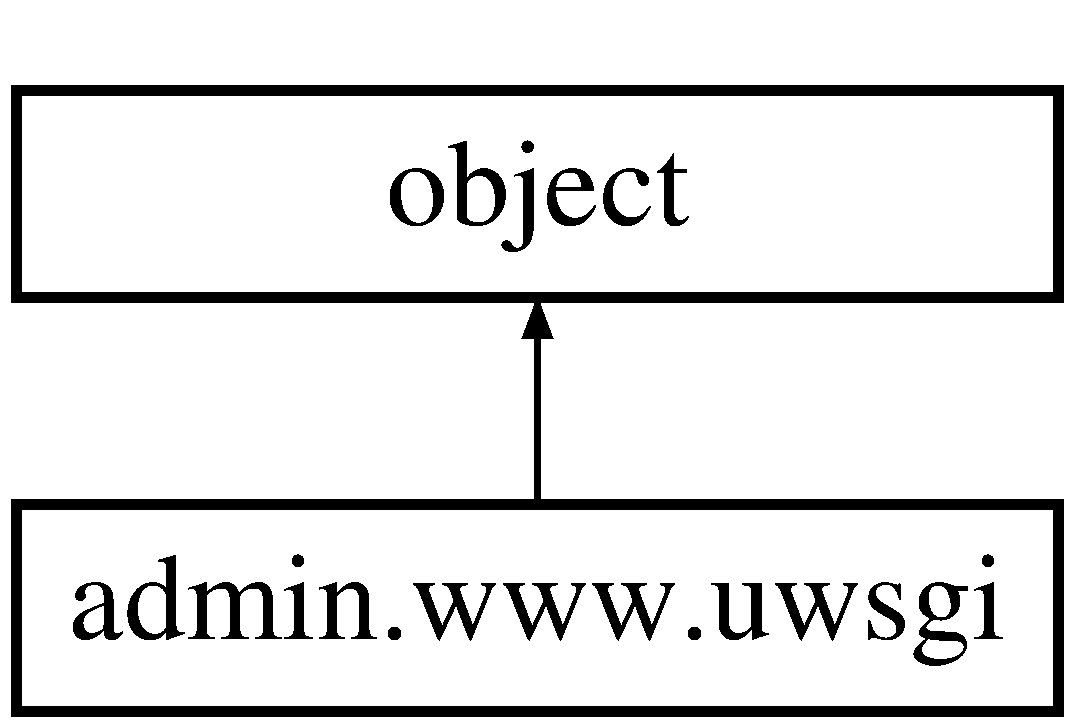
\includegraphics[height=2.000000cm]{db/de4/classadmin_1_1www_1_1uwsgi}
\end{center}
\end{figure}
\subsection*{Public Member Functions}
\begin{DoxyCompactItemize}
\item 
def \hyperlink{classadmin_1_1www_1_1uwsgi_ab5860b95c90e736ad96fb7273efa10a5}{run}
\begin{DoxyCompactList}\small\item\em Run (or Reload) u\-W\-S\-G\-I server. \end{DoxyCompactList}\item 
def \hyperlink{classadmin_1_1www_1_1uwsgi_a01b2b5c841e2da98a5e88286de95bd05}{stop}
\begin{DoxyCompactList}\small\item\em Stop u\-W\-S\-G\-I server. \end{DoxyCompactList}\end{DoxyCompactItemize}
\subsection*{Static Private Member Functions}
\begin{DoxyCompactItemize}
\item 
def \hyperlink{classadmin_1_1www_1_1uwsgi_aefa1ab9824e26e8da07141806cd69ed7}{\-\_\-pidfile}
\begin{DoxyCompactList}\small\item\em Return u\-W\-S\-G\-I pid file from app name. \end{DoxyCompactList}\end{DoxyCompactItemize}


\subsection{Detailed Description}
u\-W\-S\-G\-I server. 

\begin{DoxySeeAlso}{See Also}
\href{https://uwsgi.readthedocs.org/en/latest/index.html}{\tt https\-://uwsgi.\-readthedocs.\-org/en/latest/index.\-html} 
\end{DoxySeeAlso}
\begin{DoxySince}{Since}
u\-W\-S\-G\-I 2.\-0.\-6 
\end{DoxySince}


Definition at line 436 of file admin.\-py.



\subsection{Member Function Documentation}
\hypertarget{classadmin_1_1www_1_1uwsgi_aefa1ab9824e26e8da07141806cd69ed7}{\index{admin\-::www\-::uwsgi@{admin\-::www\-::uwsgi}!\-\_\-pidfile@{\-\_\-pidfile}}
\index{\-\_\-pidfile@{\-\_\-pidfile}!admin::www::uwsgi@{admin\-::www\-::uwsgi}}
\subsubsection[{\-\_\-pidfile}]{\setlength{\rightskip}{0pt plus 5cm}def admin.\-www.\-uwsgi.\-\_\-pidfile (
\begin{DoxyParamCaption}
\item[{}]{app}
\end{DoxyParamCaption}
)\hspace{0.3cm}{\ttfamily [static]}, {\ttfamily [private]}}}\label{classadmin_1_1www_1_1uwsgi_aefa1ab9824e26e8da07141806cd69ed7}


Return u\-W\-S\-G\-I pid file from app name. 


\begin{DoxyParams}{Parameters}
{\em app} & app name \\
\hline
\end{DoxyParams}


Definition at line 557 of file admin.\-py.

\hypertarget{classadmin_1_1www_1_1uwsgi_ab5860b95c90e736ad96fb7273efa10a5}{\index{admin\-::www\-::uwsgi@{admin\-::www\-::uwsgi}!run@{run}}
\index{run@{run}!admin::www::uwsgi@{admin\-::www\-::uwsgi}}
\subsubsection[{run}]{\setlength{\rightskip}{0pt plus 5cm}def admin.\-www.\-uwsgi.\-run (
\begin{DoxyParamCaption}
\item[{}]{cls, }
\item[{}]{app, }
\item[{}]{addr, }
\item[{}]{init = {\ttfamily False}, }
\item[{}]{gateway = {\ttfamily False}}
\end{DoxyParamCaption}
)}}\label{classadmin_1_1www_1_1uwsgi_ab5860b95c90e736ad96fb7273efa10a5}


Run (or Reload) u\-W\-S\-G\-I server. 


\begin{DoxyParams}{Parameters}
{\em app} & app (absolute) path \\
\hline
{\em addr} & u\-W\-S\-G\-I server address \\
\hline
{\em init} & True for adding to init system \\
\hline
{\em gateway} & True for internal gateway \\
\hline
\end{DoxyParams}

\begin{DoxyExceptions}{Exceptions}
{\em Value\-Error} & -\/ app path not absolute path \\
\hline
{\em Admin\-Error(subprocess.\-Called\-Process\-Error)} & -\/ shell error \\
\hline
{\em I\-O\-Error} & -\/ configuration file error\\
\hline
\end{DoxyExceptions}
N\-O\-T\-E\-: Before run u\-W\-S\-G\-I with Django, make sure that Django project actually works\-: \begin{DoxyVerb}python manage.py runserver 0.0.0.0:8000
\end{DoxyVerb}


\begin{DoxySeeAlso}{See Also}
\href{https://www.djangoproject.com/}{\tt https\-://www.\-djangoproject.\-com/} 
\end{DoxySeeAlso}
\begin{DoxySince}{Since}
Django 1.\-7 

Python 3.\-2 
\end{DoxySince}


Definition at line 457 of file admin.\-py.

\hypertarget{classadmin_1_1www_1_1uwsgi_a01b2b5c841e2da98a5e88286de95bd05}{\index{admin\-::www\-::uwsgi@{admin\-::www\-::uwsgi}!stop@{stop}}
\index{stop@{stop}!admin::www::uwsgi@{admin\-::www\-::uwsgi}}
\subsubsection[{stop}]{\setlength{\rightskip}{0pt plus 5cm}def admin.\-www.\-uwsgi.\-stop (
\begin{DoxyParamCaption}
\item[{}]{cls, }
\item[{}]{app}
\end{DoxyParamCaption}
)}}\label{classadmin_1_1www_1_1uwsgi_a01b2b5c841e2da98a5e88286de95bd05}


Stop u\-W\-S\-G\-I server. 


\begin{DoxyParams}{Parameters}
{\em app} & app (absolute) path \\
\hline
\end{DoxyParams}

\begin{DoxyExceptions}{Exceptions}
{\em Admin\-Error(subprocess.\-Called\-Process\-Error)} & -\/ shell error \\
\hline
\end{DoxyExceptions}


Definition at line 546 of file admin.\-py.



The documentation for this class was generated from the following file\-:\begin{DoxyCompactItemize}
\item 
\hyperlink{admin_8py}{admin.\-py}\end{DoxyCompactItemize}

\hypertarget{classadmin_1_1www}{\section{admin.\-www Class Reference}
\label{classadmin_1_1www}\index{admin.\-www@{admin.\-www}}
}


W\-W\-W (Internet) tools.  


Inheritance diagram for admin.\-www\-:\begin{figure}[H]
\begin{center}
\leavevmode
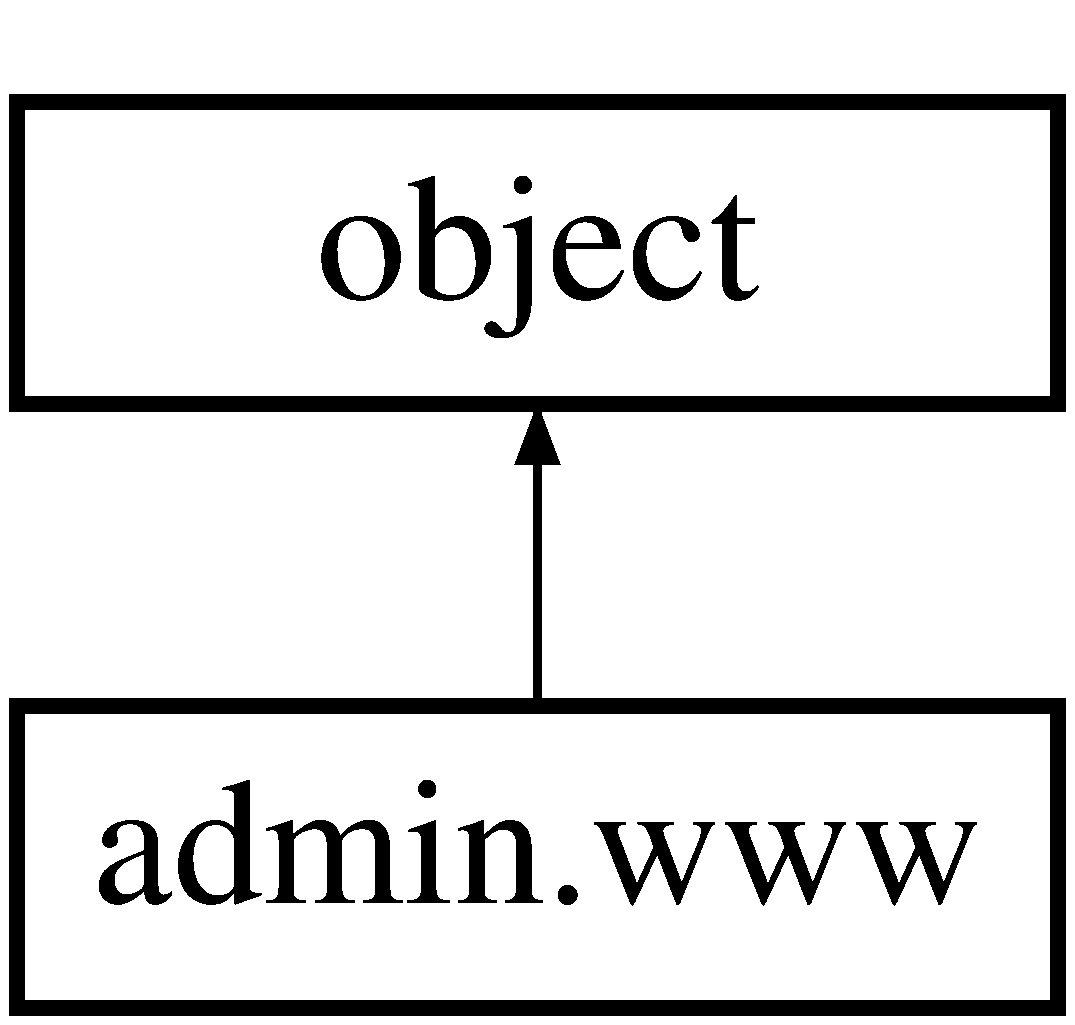
\includegraphics[height=2.000000cm]{d6/dae/classadmin_1_1www}
\end{center}
\end{figure}
\subsection*{Classes}
\begin{DoxyCompactItemize}
\item 
class \hyperlink{classadmin_1_1www_1_1nginx}{nginx}
\begin{DoxyCompactList}\small\item\em nginx server. \end{DoxyCompactList}\item 
class \hyperlink{classadmin_1_1www_1_1uwsgi}{uwsgi}
\begin{DoxyCompactList}\small\item\em u\-W\-S\-G\-I server. \end{DoxyCompactList}\end{DoxyCompactItemize}
\subsection*{Static Public Member Functions}
\begin{DoxyCompactItemize}
\item 
def \hyperlink{classadmin_1_1www_a7a25fbce0b213fb06adc0e8602a980d7}{setup}
\begin{DoxyCompactList}\small\item\em Setup W\-W\-W. \end{DoxyCompactList}\end{DoxyCompactItemize}
\subsection*{Static Public Attributes}
\begin{DoxyCompactItemize}
\item 
string \hyperlink{classadmin_1_1www_a970be68a3aafd5e7847083f756041f51}{root} = '/var/spool/\hyperlink{classadmin_1_1www}{www}'
\item 
string \hyperlink{classadmin_1_1www_a5ea11af52a64e25886b747ac675827a5}{uwsgi\-\_\-log\-\_\-root} = '/var/log/\hyperlink{classadmin_1_1www_1_1uwsgi}{uwsgi}'
\item 
string \hyperlink{classadmin_1_1www_a83f646dac924f1827dd990dcb541ebb6}{user} = '\hyperlink{classadmin_1_1www}{www}-\/data'
\item 
string \hyperlink{classadmin_1_1www_a05d4d076f879b3a22ae28f82d2bb6895}{group} = 'adm'
\end{DoxyCompactItemize}


\subsection{Detailed Description}
W\-W\-W (Internet) tools. 

This module contains functions and classes for Internet, including\-:


\begin{DoxyItemize}
\item root, uwsgi\-\_\-root\-\_\-log
\item user, group
\item uwsgi
\item nginx 
\end{DoxyItemize}

Definition at line 403 of file admin.\-py.



\subsection{Member Function Documentation}
\hypertarget{classadmin_1_1www_a7a25fbce0b213fb06adc0e8602a980d7}{\index{admin\-::www@{admin\-::www}!setup@{setup}}
\index{setup@{setup}!admin::www@{admin\-::www}}
\subsubsection[{setup}]{\setlength{\rightskip}{0pt plus 5cm}def admin.\-www.\-setup (
\begin{DoxyParamCaption}
\item[{}]{root = {\ttfamily None}, }
\item[{}]{uwsgi\-\_\-log\-\_\-root = {\ttfamily None}, }
\item[{}]{user = {\ttfamily None}, }
\item[{}]{group = {\ttfamily None}}
\end{DoxyParamCaption}
)\hspace{0.3cm}{\ttfamily [static]}}}\label{classadmin_1_1www_a7a25fbce0b213fb06adc0e8602a980d7}


Setup W\-W\-W. 


\begin{DoxyParams}{Parameters}
{\em root} & root path of W\-W\-W \\
\hline
{\em uwsgi\-\_\-log\-\_\-root} & root path of u\-W\-S\-G\-I log \\
\hline
{\em user} & user of W\-W\-W \\
\hline
{\em group} & group of W\-W\-W \\
\hline
\end{DoxyParams}

\begin{DoxyExceptions}{Exceptions}
{\em \hyperlink{classadmin_1_1AdminError}{Admin\-Error}} & -\/ shell error \\
\hline
\end{DoxyExceptions}


Definition at line 419 of file admin.\-py.



\subsection{Member Data Documentation}
\hypertarget{classadmin_1_1www_a05d4d076f879b3a22ae28f82d2bb6895}{\index{admin\-::www@{admin\-::www}!group@{group}}
\index{group@{group}!admin::www@{admin\-::www}}
\subsubsection[{group}]{\setlength{\rightskip}{0pt plus 5cm}string admin.\-www.\-group = 'adm'\hspace{0.3cm}{\ttfamily [static]}}}\label{classadmin_1_1www_a05d4d076f879b3a22ae28f82d2bb6895}


Definition at line 408 of file admin.\-py.

\hypertarget{classadmin_1_1www_a970be68a3aafd5e7847083f756041f51}{\index{admin\-::www@{admin\-::www}!root@{root}}
\index{root@{root}!admin::www@{admin\-::www}}
\subsubsection[{root}]{\setlength{\rightskip}{0pt plus 5cm}string admin.\-www.\-root = '/var/spool/{\bf www}'\hspace{0.3cm}{\ttfamily [static]}}}\label{classadmin_1_1www_a970be68a3aafd5e7847083f756041f51}


Definition at line 405 of file admin.\-py.

\hypertarget{classadmin_1_1www_a83f646dac924f1827dd990dcb541ebb6}{\index{admin\-::www@{admin\-::www}!user@{user}}
\index{user@{user}!admin::www@{admin\-::www}}
\subsubsection[{user}]{\setlength{\rightskip}{0pt plus 5cm}string admin.\-www.\-user = '{\bf www}-\/data'\hspace{0.3cm}{\ttfamily [static]}}}\label{classadmin_1_1www_a83f646dac924f1827dd990dcb541ebb6}


Definition at line 407 of file admin.\-py.

\hypertarget{classadmin_1_1www_a5ea11af52a64e25886b747ac675827a5}{\index{admin\-::www@{admin\-::www}!uwsgi\-\_\-log\-\_\-root@{uwsgi\-\_\-log\-\_\-root}}
\index{uwsgi\-\_\-log\-\_\-root@{uwsgi\-\_\-log\-\_\-root}!admin::www@{admin\-::www}}
\subsubsection[{uwsgi\-\_\-log\-\_\-root}]{\setlength{\rightskip}{0pt plus 5cm}string admin.\-www.\-uwsgi\-\_\-log\-\_\-root = '/var/log/{\bf uwsgi}'\hspace{0.3cm}{\ttfamily [static]}}}\label{classadmin_1_1www_a5ea11af52a64e25886b747ac675827a5}


Definition at line 406 of file admin.\-py.



The documentation for this class was generated from the following file\-:\begin{DoxyCompactItemize}
\item 
\hyperlink{admin_8py}{admin.\-py}\end{DoxyCompactItemize}

\chapter{File Documentation}
\hypertarget{____init_____8py}{\section{admin/\-\_\-\-\_\-init\-\_\-\-\_\-.py File Reference}
\label{____init_____8py}\index{admin/\-\_\-\-\_\-init\-\_\-\-\_\-.\-py@{admin/\-\_\-\-\_\-init\-\_\-\-\_\-.\-py}}
}
\subsection*{Classes}
\begin{DoxyCompactItemize}
\item 
class \hyperlink{classadmin_1_1ConfigFile}{admin.\-Config\-File}
\begin{DoxyCompactList}\small\item\em Configuration file. \end{DoxyCompactList}\item 
class \hyperlink{classadmin_1_1AdminTestCase}{admin.\-Admin\-Test\-Case}
\end{DoxyCompactItemize}
\subsection*{Namespaces}
\begin{DoxyCompactItemize}
\item 
\hyperlink{namespaceadmin}{admin}
\end{DoxyCompactItemize}
\subsection*{Functions}
\begin{DoxyCompactItemize}
\item 
def \hyperlink{namespaceadmin_ae1e80d1a965f6551fa95ff379ba2b0cd}{admin.\-error}
\begin{DoxyCompactList}\small\item\em Print error messages. \end{DoxyCompactList}\item 
def \hyperlink{namespaceadmin_a575bcc44ebed9e68574ccb636a66a4d2}{admin.\-debug}
\begin{DoxyCompactList}\small\item\em Print debugging message. \end{DoxyCompactList}\item 
def \hyperlink{namespaceadmin_ae1dbeff3e935d67ed99b95eb814c9a11}{admin.\-update\-\_\-seq\-\_\-type}
\begin{DoxyCompactList}\small\item\em Update type of all elements in specific sequence. \end{DoxyCompactList}\item 
def \hyperlink{namespaceadmin_a8b0cb2905f04979a2db7cf3bb181ad00}{admin.\-force\-\_\-remove}
\begin{DoxyCompactList}\small\item\em Command {\ttfamily rm -\/f}. \end{DoxyCompactList}\item 
def \hyperlink{namespaceadmin_a186685a5e2120c71362c46b35f0705c3}{admin.\-eintr\-\_\-retry}
\begin{DoxyCompactList}\small\item\em Restart a system call interrupted by {\ttfamily E\-I\-N\-T\-R}. \end{DoxyCompactList}\item 
def \hyperlink{namespaceadmin_a2605170b60fdae0f26432f209ed71f49}{admin.\-decode\-\_\-version}
\begin{DoxyCompactList}\small\item\em Decode version information string. \end{DoxyCompactList}\item 
def \hyperlink{namespaceadmin_a89c4e2a6cc63b64d27825da9eb414b98}{admin.\-match\-\_\-version}
\begin{DoxyCompactList}\small\item\em Match the specific version. \end{DoxyCompactList}\item 
def \hyperlink{namespaceadmin_ae034627a9fca691b23ee55d255113a81}{admin.\-read\-\_\-lines}
\begin{DoxyCompactList}\small\item\em Read specific line(s) with line number(s). \end{DoxyCompactList}\end{DoxyCompactItemize}
\subsection*{Variables}
\begin{DoxyCompactItemize}
\item 
tuple \hyperlink{namespaceadmin_acbbc1dce90a9452383bd52c69b4a7489}{admin.\-Version} = namedtuple('Version', 'major, minor, patch')
\end{DoxyCompactItemize}

\hypertarget{thread_2____init_____8py}{\section{\-\_\-cookbook/thread/\-\_\-\-\_\-init\-\_\-\-\_\-.py File Reference}
\label{thread_2____init_____8py}\index{\-\_\-cookbook/thread/\-\_\-\-\_\-init\-\_\-\-\_\-.\-py@{\-\_\-cookbook/thread/\-\_\-\-\_\-init\-\_\-\-\_\-.\-py}}
}
\subsection*{Namespaces}
\begin{DoxyCompactItemize}
\item 
\hyperlink{namespace__cookbook_1_1thread}{\-\_\-cookbook.\-thread}
\end{DoxyCompactItemize}

\hypertarget{__doctest_8py}{\section{\-\_\-cookbook/\-\_\-doctest.py File Reference}
\label{__doctest_8py}\index{\-\_\-cookbook/\-\_\-doctest.\-py@{\-\_\-cookbook/\-\_\-doctest.\-py}}
}
\subsection*{Namespaces}
\begin{DoxyCompactItemize}
\item 
\hyperlink{namespace__cookbook_1_1__doctest}{\-\_\-cookbook.\-\_\-doctest}
\end{DoxyCompactItemize}
\subsection*{Functions}
\begin{DoxyCompactItemize}
\item 
def \hyperlink{namespace__cookbook_1_1__doctest_a2b5f4f492189ea465a7e682adfdc1083}{\-\_\-cookbook.\-\_\-doctest.\-func\-\_\-1}
\item 
def \hyperlink{namespace__cookbook_1_1__doctest_aaf8b2718413a6692d2e365e00ca9ba0b}{\-\_\-cookbook.\-\_\-doctest.\-func\-\_\-2}
\item 
def \hyperlink{namespace__cookbook_1_1__doctest_a18f8bfc06597191f2fe2d581586e897b}{\-\_\-cookbook.\-\_\-doctest.\-func\-\_\-3}
\item 
def \hyperlink{namespace__cookbook_1_1__doctest_a476ec0259fc7f1ac3c794c93a435d161}{\-\_\-cookbook.\-\_\-doctest.\-func\-\_\-4}
\end{DoxyCompactItemize}

\hypertarget{__unittest_8py}{\section{\-\_\-cookbook/\-\_\-unittest.py File Reference}
\label{__unittest_8py}\index{\-\_\-cookbook/\-\_\-unittest.\-py@{\-\_\-cookbook/\-\_\-unittest.\-py}}
}
\subsection*{Classes}
\begin{DoxyCompactItemize}
\item 
class \hyperlink{class__cookbook_1_1__unittest_1_1__UnitTestTestCase}{\-\_\-cookbook.\-\_\-unittest.\-\_\-\-Unit\-Test\-Test\-Case}
\end{DoxyCompactItemize}
\subsection*{Namespaces}
\begin{DoxyCompactItemize}
\item 
\hyperlink{namespace__cookbook_1_1__unittest}{\-\_\-cookbook.\-\_\-unittest}
\end{DoxyCompactItemize}
\subsection*{Functions}
\begin{DoxyCompactItemize}
\item 
def \hyperlink{namespace__cookbook_1_1__unittest_a17e6d30389570d1c07541e5ea2f27719}{\-\_\-cookbook.\-\_\-unittest.\-func\-\_\-1}
\item 
def \hyperlink{namespace__cookbook_1_1__unittest_a8ebeb354b9c5c6507083565546b42e42}{\-\_\-cookbook.\-\_\-unittest.\-func\-\_\-2}
\item 
def \hyperlink{namespace__cookbook_1_1__unittest_a631f2b683949a2db9f953d07811307f7}{\-\_\-cookbook.\-\_\-unittest.\-func\-\_\-3}
\end{DoxyCompactItemize}

\hypertarget{context__manager_8py}{\section{\-\_\-cookbook/context\-\_\-manager.py File Reference}
\label{context__manager_8py}\index{\-\_\-cookbook/context\-\_\-manager.\-py@{\-\_\-cookbook/context\-\_\-manager.\-py}}
}
\subsection*{Classes}
\begin{DoxyCompactItemize}
\item 
class \hyperlink{class__cookbook_1_1context__manager_1_1MyContextManagerWithDecorator}{\-\_\-cookbook.\-context\-\_\-manager.\-My\-Context\-Manager\-With\-Decorator}
\end{DoxyCompactItemize}
\subsection*{Namespaces}
\begin{DoxyCompactItemize}
\item 
\hyperlink{namespace__cookbook_1_1context__manager}{\-\_\-cookbook.\-context\-\_\-manager}
\end{DoxyCompactItemize}
\subsection*{Functions}
\begin{DoxyCompactItemize}
\item 
def \hyperlink{namespace__cookbook_1_1context__manager_aafbcdbb97984af3f9b06301a3c27f8fd}{\-\_\-cookbook.\-context\-\_\-manager.\-opening}
\item 
def \hyperlink{namespace__cookbook_1_1context__manager_a05fb8dadba363071eaf9fa4adfa2625a}{\-\_\-cookbook.\-context\-\_\-manager.\-closing}
\item 
def \hyperlink{namespace__cookbook_1_1context__manager_a2e71ffab9a602c353f47bdcf9785f7c0}{\-\_\-cookbook.\-context\-\_\-manager.\-test}
\end{DoxyCompactItemize}

\hypertarget{file_8py}{\section{\-\_\-cookbook/file.py File Reference}
\label{file_8py}\index{\-\_\-cookbook/file.\-py@{\-\_\-cookbook/file.\-py}}
}
\subsection*{Namespaces}
\begin{DoxyCompactItemize}
\item 
\hyperlink{namespace__cookbook_1_1file}{\-\_\-cookbook.\-file}
\end{DoxyCompactItemize}
\subsection*{Functions}
\begin{DoxyCompactItemize}
\item 
def \hyperlink{namespace__cookbook_1_1file_a34fcd24232dcbcdf63ff458bea388f17}{\-\_\-cookbook.\-file.\-test\-\_\-bin\-\_\-io}
\item 
def \hyperlink{namespace__cookbook_1_1file_a7677b9761322c16cc2353cd670e3af85}{\-\_\-cookbook.\-file.\-test\-\_\-mmap}
\end{DoxyCompactItemize}

\hypertarget{find_8py}{\section{\-\_\-cookbook/find.py File Reference}
\label{find_8py}\index{\-\_\-cookbook/find.\-py@{\-\_\-cookbook/find.\-py}}
}
\subsection*{Namespaces}
\begin{DoxyCompactItemize}
\item 
\hyperlink{namespace__cookbook_1_1find}{\-\_\-cookbook.\-find}
\end{DoxyCompactItemize}
\subsection*{Variables}
\begin{DoxyCompactItemize}
\item 
list \hyperlink{namespace__cookbook_1_1find_a2b63929bb9d60c107a94ede0430dd2c6}{\-\_\-cookbook.\-find.\-seq} = \mbox{[}1, 8, 2, 23, 7, -\/2, 18, 23, 42, 37, 2\mbox{]}
\item 
list \hyperlink{namespace__cookbook_1_1find_a687bf0a1e78a409f1fe7c38291568113}{\-\_\-cookbook.\-find.\-list\-\_\-of\-\_\-dict}
\item 
dictionary \hyperlink{namespace__cookbook_1_1find_ad505b83a6410c8ac07573995e48df338}{\-\_\-cookbook.\-find.\-d}
\end{DoxyCompactItemize}

\hypertarget{format_8py}{\section{\-\_\-cookbook/format.py File Reference}
\label{format_8py}\index{\-\_\-cookbook/format.\-py@{\-\_\-cookbook/format.\-py}}
}
\subsection*{Namespaces}
\begin{DoxyCompactItemize}
\item 
\hyperlink{namespace__cookbook_1_1format}{\-\_\-cookbook.\-format}
\end{DoxyCompactItemize}
\subsection*{Functions}
\begin{DoxyCompactItemize}
\item 
def \hyperlink{namespace__cookbook_1_1format_ae20d8728a10632bc8452d59c2f370b6f}{\-\_\-cookbook.\-format.\-test\-\_\-float\-\_\-format}
\item 
def \hyperlink{namespace__cookbook_1_1format_a842708e728d2204d2e5314e719e49ea5}{\-\_\-cookbook.\-format.\-test\-\_\-int\-\_\-format}
\end{DoxyCompactItemize}

\hypertarget{func__param_8py}{\section{\-\_\-cookbook/func\-\_\-param.py File Reference}
\label{func__param_8py}\index{\-\_\-cookbook/func\-\_\-param.\-py@{\-\_\-cookbook/func\-\_\-param.\-py}}
}
\subsection*{Namespaces}
\begin{DoxyCompactItemize}
\item 
\hyperlink{namespace__cookbook_1_1func__param}{\-\_\-cookbook.\-func\-\_\-param}
\end{DoxyCompactItemize}
\subsection*{Functions}
\begin{DoxyCompactItemize}
\item 
def \hyperlink{namespace__cookbook_1_1func__param_a7ac8623dbed6df5d65129f0326b167a0}{\-\_\-cookbook.\-func\-\_\-param.\-func\-\_\-default\-\_\-value}
\item 
def \hyperlink{namespace__cookbook_1_1func__param_afc9ae01c0be44ec44fbb10b2ae6da082}{\-\_\-cookbook.\-func\-\_\-param.\-func\-\_\-unpack\-\_\-args}
\item 
def \hyperlink{namespace__cookbook_1_1func__param_a2c71d6b96799766585c48cfca1b92616}{\-\_\-cookbook.\-func\-\_\-param.\-func\-\_\-vargs}
\end{DoxyCompactItemize}

\hypertarget{loop_8py}{\section{\-\_\-cookbook/loop.py File Reference}
\label{loop_8py}\index{\-\_\-cookbook/loop.\-py@{\-\_\-cookbook/loop.\-py}}
}
\subsection*{Classes}
\begin{DoxyCompactItemize}
\item 
class \hyperlink{class__cookbook_1_1loop_1_1MyIterator}{\-\_\-cookbook.\-loop.\-My\-Iterator}
\end{DoxyCompactItemize}
\subsection*{Namespaces}
\begin{DoxyCompactItemize}
\item 
\hyperlink{namespace__cookbook_1_1loop}{\-\_\-cookbook.\-loop}
\end{DoxyCompactItemize}
\subsection*{Functions}
\begin{DoxyCompactItemize}
\item 
def \hyperlink{namespace__cookbook_1_1loop_a9a2442115a97e67514ca641a1123a54b}{\-\_\-cookbook.\-loop.\-my\-\_\-generator}
\item 
def \hyperlink{namespace__cookbook_1_1loop_a0378ad6d1d792ff3aee7ea1bc6bd7e3b}{\-\_\-cookbook.\-loop.\-test\-\_\-filter}
\end{DoxyCompactItemize}
\subsection*{Variables}
\begin{DoxyCompactItemize}
\item 
list \hyperlink{namespace__cookbook_1_1loop_a5de56a796b0d1e61c000d4258c4174c4}{\-\_\-cookbook.\-loop.\-seq} = \mbox{[}$\,$\mbox{]}
\item 
list \hyperlink{namespace__cookbook_1_1loop_a65ecd74c88616db43b44e064e12bb30a}{\-\_\-cookbook.\-loop.\-words} = \mbox{[}$\,$\mbox{]}
\item 
dictionary \hyperlink{namespace__cookbook_1_1loop_a6e274a42a5573ac12fed6a6f9c318fe0}{\-\_\-cookbook.\-loop.\-mydict} = \{\}
\end{DoxyCompactItemize}

\hypertarget{my__pyunit_8py}{\section{\-\_\-cookbook/my\-\_\-pyunit.py File Reference}
\label{my__pyunit_8py}\index{\-\_\-cookbook/my\-\_\-pyunit.\-py@{\-\_\-cookbook/my\-\_\-pyunit.\-py}}
}
\subsection*{Classes}
\begin{DoxyCompactItemize}
\item 
class \hyperlink{class__cookbook_1_1my__pyunit_1_1TestCase}{\-\_\-cookbook.\-my\-\_\-pyunit.\-Test\-Case}
\item 
class \hyperlink{class__cookbook_1_1my__pyunit_1_1TestSuite}{\-\_\-cookbook.\-my\-\_\-pyunit.\-Test\-Suite}
\item 
class \hyperlink{class__cookbook_1_1my__pyunit_1_1MyPyUnitTest}{\-\_\-cookbook.\-my\-\_\-pyunit.\-My\-Py\-Unit\-Test}
\end{DoxyCompactItemize}
\subsection*{Namespaces}
\begin{DoxyCompactItemize}
\item 
\hyperlink{namespace__cookbook_1_1my__pyunit}{\-\_\-cookbook.\-my\-\_\-pyunit}
\end{DoxyCompactItemize}
\subsection*{Variables}
\begin{DoxyCompactItemize}
\item 
list \hyperlink{namespace__cookbook_1_1my__pyunit_a1650ca62d0d76280d5c2a10f66c08aa8}{\-\_\-cookbook.\-my\-\_\-pyunit.\-\_\-test\-\_\-suite} = \mbox{[}$\,$\mbox{]}
\item 
tuple \hyperlink{namespace__cookbook_1_1my__pyunit_a0d863c11cc0e82383e086450f052ecea}{\-\_\-cookbook.\-my\-\_\-pyunit.\-suite} = Test\-Suite()
\end{DoxyCompactItemize}

\hypertarget{network_8py}{\section{\-\_\-cookbook/network.py File Reference}
\label{network_8py}\index{\-\_\-cookbook/network.\-py@{\-\_\-cookbook/network.\-py}}
}
\subsection*{Classes}
\begin{DoxyCompactItemize}
\item 
class \hyperlink{class__cookbook_1_1network_1_1MyTCPServer}{\-\_\-cookbook.\-network.\-My\-T\-C\-P\-Server}
\item 
class \hyperlink{class__cookbook_1_1network_1_1MyUDPServer}{\-\_\-cookbook.\-network.\-My\-U\-D\-P\-Server}
\item 
class \hyperlink{class__cookbook_1_1network_1_1MyTCPHandler}{\-\_\-cookbook.\-network.\-My\-T\-C\-P\-Handler}
\end{DoxyCompactItemize}
\subsection*{Namespaces}
\begin{DoxyCompactItemize}
\item 
\hyperlink{namespace__cookbook_1_1network}{\-\_\-cookbook.\-network}
\end{DoxyCompactItemize}
\subsection*{Functions}
\begin{DoxyCompactItemize}
\item 
def \hyperlink{namespace__cookbook_1_1network_a3d1bb77e5f5c2b7ad21cb41f8e76ff2b}{\-\_\-cookbook.\-network.\-\_\-eintr\-\_\-retry}
\item 
def \hyperlink{namespace__cookbook_1_1network_afda73ac0991cd562372fb04f9d76e25d}{\-\_\-cookbook.\-network.\-tcp\-\_\-client}
\item 
def \hyperlink{namespace__cookbook_1_1network_ad136212440d95bb9b1fdaac0cca36668}{\-\_\-cookbook.\-network.\-udp\-\_\-client}
\item 
def \hyperlink{namespace__cookbook_1_1network_ae7f29425dec008925037e722e4a0e561}{\-\_\-cookbook.\-network.\-tcp\-\_\-server}
\end{DoxyCompactItemize}
\subsection*{Variables}
\begin{DoxyCompactItemize}
\item 
tuple \hyperlink{namespace__cookbook_1_1network_af47f70f9a1bf283ae86e02e67cf9c91a}{\-\_\-cookbook.\-network.\-srv} = My\-T\-C\-P\-Server(('', 10000))
\item 
tuple \hyperlink{namespace__cookbook_1_1network_a07395291bd1e407e4fdf8850535b5427}{\-\_\-cookbook.\-network.\-srv\-\_\-addr} = ('localhost', 10000)
\end{DoxyCompactItemize}

\hypertarget{OOP_8py}{\section{\-\_\-cookbook/\-O\-O\-P.py File Reference}
\label{OOP_8py}\index{\-\_\-cookbook/\-O\-O\-P.\-py@{\-\_\-cookbook/\-O\-O\-P.\-py}}
}
\subsection*{Classes}
\begin{DoxyCompactItemize}
\item 
class \hyperlink{class__cookbook_1_1OOP_1_1A}{\-\_\-cookbook.\-O\-O\-P.\-A}
\item 
class \hyperlink{class__cookbook_1_1OOP_1_1B}{\-\_\-cookbook.\-O\-O\-P.\-B}
\end{DoxyCompactItemize}
\subsection*{Namespaces}
\begin{DoxyCompactItemize}
\item 
\hyperlink{namespace__cookbook_1_1OOP}{\-\_\-cookbook.\-O\-O\-P}
\end{DoxyCompactItemize}

\hypertarget{sort_8py}{\section{\-\_\-cookbook/sort.py File Reference}
\label{sort_8py}\index{\-\_\-cookbook/sort.\-py@{\-\_\-cookbook/sort.\-py}}
}
\subsection*{Classes}
\begin{DoxyCompactItemize}
\item 
class \hyperlink{class__cookbook_1_1sort_1_1App}{\-\_\-cookbook.\-sort.\-App}
\end{DoxyCompactItemize}
\subsection*{Namespaces}
\begin{DoxyCompactItemize}
\item 
\hyperlink{namespace__cookbook_1_1sort}{\-\_\-cookbook.\-sort}
\end{DoxyCompactItemize}
\subsection*{Variables}
\begin{DoxyCompactItemize}
\item 
list \hyperlink{namespace__cookbook_1_1sort_a75232840573a2c0ea5f03c47fc06f540}{\-\_\-cookbook.\-sort.\-d}
\item 
list \hyperlink{namespace__cookbook_1_1sort_a0f8929d439af8acc1f7c8beb0c62bc91}{\-\_\-cookbook.\-sort.\-apps} = \mbox{[}App(1), App(2), App(3)\mbox{]}
\end{DoxyCompactItemize}

\hypertarget{text__pattern_8py}{\section{\-\_\-cookbook/text\-\_\-pattern.py File Reference}
\label{text__pattern_8py}\index{\-\_\-cookbook/text\-\_\-pattern.\-py@{\-\_\-cookbook/text\-\_\-pattern.\-py}}
}
\subsection*{Namespaces}
\begin{DoxyCompactItemize}
\item 
\hyperlink{namespace__cookbook_1_1text__pattern}{\-\_\-cookbook.\-text\-\_\-pattern}
\end{DoxyCompactItemize}
\subsection*{Functions}
\begin{DoxyCompactItemize}
\item 
def \hyperlink{namespace__cookbook_1_1text__pattern_a99aed64f324c4d7bd5ee90c0aadca9d4}{\-\_\-cookbook.\-text\-\_\-pattern.\-test\-\_\-re\-\_\-pattern}
\item 
def \hyperlink{namespace__cookbook_1_1text__pattern_ad7e6795f9dd1ab31ff51db9c61c3f1e1}{\-\_\-cookbook.\-text\-\_\-pattern.\-test\-\_\-shell\-\_\-pattern}
\end{DoxyCompactItemize}

\hypertarget{__queue_8py}{\section{\-\_\-cookbook/thread/\-\_\-queue.py File Reference}
\label{__queue_8py}\index{\-\_\-cookbook/thread/\-\_\-queue.\-py@{\-\_\-cookbook/thread/\-\_\-queue.\-py}}
}
\subsection*{Classes}
\begin{DoxyCompactItemize}
\item 
class \hyperlink{class__cookbook_1_1thread_1_1__queue_1_1Producer}{\-\_\-cookbook.\-thread.\-\_\-queue.\-Producer}
\item 
class \hyperlink{class__cookbook_1_1thread_1_1__queue_1_1Cusumer}{\-\_\-cookbook.\-thread.\-\_\-queue.\-Cusumer}
\end{DoxyCompactItemize}
\subsection*{Namespaces}
\begin{DoxyCompactItemize}
\item 
\hyperlink{namespace__cookbook_1_1thread_1_1__queue}{\-\_\-cookbook.\-thread.\-\_\-queue}
\end{DoxyCompactItemize}
\subsection*{Functions}
\begin{DoxyCompactItemize}
\item 
def \hyperlink{namespace__cookbook_1_1thread_1_1__queue_a4e666d288ea239711e5bfc40fd358543}{\-\_\-cookbook.\-thread.\-\_\-queue.\-test\-\_\-queue}
\end{DoxyCompactItemize}
\subsection*{Variables}
\begin{DoxyCompactItemize}
\item 
tuple \hyperlink{namespace__cookbook_1_1thread_1_1__queue_ab96e0faed9a5bf9793248aaad5d463ee}{\-\_\-cookbook.\-thread.\-\_\-queue.\-q} = queue.\-Queue(maxsize=10)
\end{DoxyCompactItemize}

\hypertarget{lock_8py}{\section{\-\_\-cookbook/thread/lock.py File Reference}
\label{lock_8py}\index{\-\_\-cookbook/thread/lock.\-py@{\-\_\-cookbook/thread/lock.\-py}}
}
\subsection*{Classes}
\begin{DoxyCompactItemize}
\item 
class \hyperlink{class__cookbook_1_1thread_1_1lock_1_1MyThread}{\-\_\-cookbook.\-thread.\-lock.\-My\-Thread}
\end{DoxyCompactItemize}
\subsection*{Namespaces}
\begin{DoxyCompactItemize}
\item 
\hyperlink{namespace__cookbook_1_1thread_1_1lock}{\-\_\-cookbook.\-thread.\-lock}
\end{DoxyCompactItemize}
\subsection*{Functions}
\begin{DoxyCompactItemize}
\item 
def \hyperlink{namespace__cookbook_1_1thread_1_1lock_afcc47eebfeeb5d0b1e7f0e7f0c8c4cf0}{\-\_\-cookbook.\-thread.\-lock.\-test\-\_\-lock}
\end{DoxyCompactItemize}
\subsection*{Variables}
\begin{DoxyCompactItemize}
\item 
list \hyperlink{namespace__cookbook_1_1thread_1_1lock_a01cd21c9f5d662e95ebfc9c4b7f8629c}{\-\_\-cookbook.\-thread.\-lock.\-share} = \mbox{[}$\,$\mbox{]}
\item 
tuple \hyperlink{namespace__cookbook_1_1thread_1_1lock_a3289d10edb64e7979ae4e31600fa6be4}{\-\_\-cookbook.\-thread.\-lock.\-lock} = threading.\-Lock()
\end{DoxyCompactItemize}

\hypertarget{my__queue_8py}{\section{\-\_\-cookbook/thread/my\-\_\-queue.py File Reference}
\label{my__queue_8py}\index{\-\_\-cookbook/thread/my\-\_\-queue.\-py@{\-\_\-cookbook/thread/my\-\_\-queue.\-py}}
}
\subsection*{Classes}
\begin{DoxyCompactItemize}
\item 
class \hyperlink{class__cookbook_1_1thread_1_1my__queue_1_1MyQueue}{\-\_\-cookbook.\-thread.\-my\-\_\-queue.\-My\-Queue}
\end{DoxyCompactItemize}
\subsection*{Namespaces}
\begin{DoxyCompactItemize}
\item 
\hyperlink{namespace__cookbook_1_1thread_1_1my__queue}{\-\_\-cookbook.\-thread.\-my\-\_\-queue}
\end{DoxyCompactItemize}
\subsection*{Functions}
\begin{DoxyCompactItemize}
\item 
def \hyperlink{namespace__cookbook_1_1thread_1_1my__queue_a09765554f193f5e1929f4a1bb49075c4}{\-\_\-cookbook.\-thread.\-my\-\_\-queue.\-test}
\end{DoxyCompactItemize}
\subsection*{Variables}
\begin{DoxyCompactItemize}
\item 
\hyperlink{namespace__cookbook_1_1thread_1_1my__queue_a2663f5c52855449734498ef4269f8e42}{\-\_\-cookbook.\-thread.\-my\-\_\-queue.\-\_\-times}
\end{DoxyCompactItemize}

\hypertarget{semaphore_8py}{\section{\-\_\-cookbook/thread/semaphore.py File Reference}
\label{semaphore_8py}\index{\-\_\-cookbook/thread/semaphore.\-py@{\-\_\-cookbook/thread/semaphore.\-py}}
}
\subsection*{Classes}
\begin{DoxyCompactItemize}
\item 
class \hyperlink{class__cookbook_1_1thread_1_1semaphore_1_1Producer}{\-\_\-cookbook.\-thread.\-semaphore.\-Producer}
\item 
class \hyperlink{class__cookbook_1_1thread_1_1semaphore_1_1Cusumer}{\-\_\-cookbook.\-thread.\-semaphore.\-Cusumer}
\end{DoxyCompactItemize}
\subsection*{Namespaces}
\begin{DoxyCompactItemize}
\item 
\hyperlink{namespace__cookbook_1_1thread_1_1semaphore}{\-\_\-cookbook.\-thread.\-semaphore}
\end{DoxyCompactItemize}
\subsection*{Functions}
\begin{DoxyCompactItemize}
\item 
def \hyperlink{namespace__cookbook_1_1thread_1_1semaphore_a5fbba75227af2444a9cd91f99d4cca94}{\-\_\-cookbook.\-thread.\-semaphore.\-test\-\_\-semaphore}
\end{DoxyCompactItemize}
\subsection*{Variables}
\begin{DoxyCompactItemize}
\item 
list \hyperlink{namespace__cookbook_1_1thread_1_1semaphore_a9a0b5a124aff3e078787972f21d297e3}{\-\_\-cookbook.\-thread.\-semaphore.\-share} = \mbox{[}$\,$\mbox{]}
\item 
int \hyperlink{namespace__cookbook_1_1thread_1_1semaphore_a67e6819d1307ed665cb515e3f47a990e}{\-\_\-cookbook.\-thread.\-semaphore.\-M\-A\-X\-\_\-\-C\-O\-U\-N\-T\-S} = 5
\item 
tuple \hyperlink{namespace__cookbook_1_1thread_1_1semaphore_a522d222885e9efd1ac70e59a9c880c8f}{\-\_\-cookbook.\-thread.\-semaphore.\-semaphore} = threading.\-Bounded\-Semaphore(M\-A\-X\-\_\-\-C\-O\-U\-N\-T\-S)
\end{DoxyCompactItemize}

\hypertarget{unpack__iterable_8py}{\section{\-\_\-cookbook/unpack\-\_\-iterable.py File Reference}
\label{unpack__iterable_8py}\index{\-\_\-cookbook/unpack\-\_\-iterable.\-py@{\-\_\-cookbook/unpack\-\_\-iterable.\-py}}
}
\subsection*{Namespaces}
\begin{DoxyCompactItemize}
\item 
\hyperlink{namespace__cookbook_1_1unpack__iterable}{\-\_\-cookbook.\-unpack\-\_\-iterable}
\end{DoxyCompactItemize}
\subsection*{Variables}
\begin{DoxyCompactItemize}
\item 
list \hyperlink{namespace__cookbook_1_1unpack__iterable_a1051db43e28f2fffb3fd98c1c990ee7b}{\-\_\-cookbook.\-unpack\-\_\-iterable.\-seq} = \mbox{[}1, 2, 3, 4, 5\mbox{]}
\end{DoxyCompactItemize}

\hypertarget{hello__uwsgi__app_8py}{\section{\-\_\-setup/hello\-\_\-uwsgi\-\_\-app.py File Reference}
\label{hello__uwsgi__app_8py}\index{\-\_\-setup/hello\-\_\-uwsgi\-\_\-app.\-py@{\-\_\-setup/hello\-\_\-uwsgi\-\_\-app.\-py}}
}
\subsection*{Namespaces}
\begin{DoxyCompactItemize}
\item 
\hyperlink{namespacehello__uwsgi__app}{hello\-\_\-uwsgi\-\_\-app}
\end{DoxyCompactItemize}
\subsection*{Functions}
\begin{DoxyCompactItemize}
\item 
def \hyperlink{namespacehello__uwsgi__app_a87c20de7f6fcc1eaa1ba7b1e5fe061be}{hello\-\_\-uwsgi\-\_\-app.\-application}
\end{DoxyCompactItemize}

\hypertarget{admin_8py}{\section{admin.\-py File Reference}
\label{admin_8py}\index{admin.\-py@{admin.\-py}}
}
\subsection*{Classes}
\begin{DoxyCompactItemize}
\item 
class \hyperlink{classadmin_1_1AdminError}{admin.\-Admin\-Error}
\begin{DoxyCompactList}\small\item\em admin error \end{DoxyCompactList}\item 
class \hyperlink{classadmin_1_1shell}{admin.\-shell}
\begin{DoxyCompactList}\small\item\em Linux shell tools. \end{DoxyCompactList}\item 
class \hyperlink{classadmin_1_1build}{admin.\-build}
\begin{DoxyCompactList}\small\item\em Build tools. \end{DoxyCompactList}\item 
class \hyperlink{classadmin_1_1www}{admin.\-www}
\begin{DoxyCompactList}\small\item\em W\-W\-W (Internet) tools. \end{DoxyCompactList}\item 
class \hyperlink{classadmin_1_1www_1_1uwsgi}{admin.\-www.\-uwsgi}
\begin{DoxyCompactList}\small\item\em u\-W\-S\-G\-I server. \end{DoxyCompactList}\item 
class \hyperlink{classadmin_1_1www_1_1nginx}{admin.\-www.\-nginx}
\begin{DoxyCompactList}\small\item\em nginx server. \end{DoxyCompactList}\item 
class \hyperlink{classadmin_1_1ConfigFile}{admin.\-Config\-File}
\begin{DoxyCompactList}\small\item\em Configuration file. \end{DoxyCompactList}\end{DoxyCompactItemize}
\subsection*{Namespaces}
\begin{DoxyCompactItemize}
\item 
\hyperlink{namespaceadmin}{admin}
\end{DoxyCompactItemize}
\subsection*{Functions}
\begin{DoxyCompactItemize}
\item 
def \hyperlink{namespaceadmin_ae1dbeff3e935d67ed99b95eb814c9a11}{admin.\-update\-\_\-seq\-\_\-type}
\begin{DoxyCompactList}\small\item\em Update type of all elements in specific sequence. \end{DoxyCompactList}\item 
def \hyperlink{namespaceadmin_a56bda7fa84a9e893fdeb0d8acd29e89b}{admin.\-\_\-setup}
\item 
def \hyperlink{namespaceadmin_a8edf8d50d5e47a6d8859c560c28ebb36}{admin.\-\_\-usage}
\end{DoxyCompactItemize}
\subsection*{Variables}
\begin{DoxyCompactItemize}
\item 
list \hyperlink{namespaceadmin_a5ed72260a120fc91cfd491f424eeb883}{admin.\-option} = sys.\-argv\mbox{[}1\mbox{]}
\item 
list \hyperlink{namespaceadmin_a88f927a5e67d8ccf759fd256f58a9411}{admin.\-app} = sys.\-argv\mbox{[}2\mbox{]}
\item 
list \hyperlink{namespaceadmin_a6320eb02d5f6324a82fe70a83901b014}{admin.\-addr} = sys.\-argv\mbox{[}3\mbox{]}
\item 
list \hyperlink{namespaceadmin_ae04b67153bc11f5b3a23e4fd760832fb}{admin.\-upstream} = sys.\-argv\mbox{[}3\mbox{]}
\item 
list \hyperlink{namespaceadmin_a311ce11d8285f485768151b9d757e478}{admin.\-project\-\_\-path} = sys.\-argv\mbox{[}2\mbox{]}
\item 
string \hyperlink{namespaceadmin_ab3c6174394fe2a906dbf095d1d83378a}{admin.\-test\-\_\-app} = '\-\_\-setup/hello\-\_\-uwsgi\-\_\-app.\-py'
\item 
string \hyperlink{namespaceadmin_a48db396eb86a22a960bba5ce65c12651}{admin.\-test\-\_\-addr} = '\-:8000'
\end{DoxyCompactItemize}

%--- End generated contents ---

% Index
\newpage
\phantomsection
\addcontentsline{toc}{chapter}{Index}
\printindex

\end{document}
